% document class -------------------------------------------
\documentclass[11pt,oneside,openright]{phdthesis}
% ----------------------------------------------------------

\usepackage{float}
\usepackage[linkcolor=black]{hyperref}
\usepackage[sorting=none, backend=biber]{biblatex}
\usepackage[T1]{fontenc}

% graphicx -----------------------------------------------------------------------------------
% The graphicx package allows to specify several paths in which to search for figures.
\usepackage{graphicx}
% --------------------------------------------------------------------------------------------

%\usepackage{amsmath}
%
%
%\usepackage[ansinew]{inputenc}
%%\usepackage[portuguese]{babel}
%\usepackage[printonlyused, withpage]{acronym}
%\usepackage{a4wide}
%\usepackage{palatino}
%\usepackage{fancyhdr}
%\usepackage{fancybox}
%\usepackage{amssymb}
%
%% biblatex ------------------------------------------------------------------------------------------
%% used to divide the bibliography into multiple parts for example per chapter or per section
%\usepackage[sorting=none, backend=biber]{biblatex}
%% ---------------------------------------------------------------------------------------------------
%
%
%\usepackage{epsfig}
%\usepackage{graphics}
%
%\usepackage{here}
%\usepackage{rotating}
%\usepackage{multirow}
%%\usepackage{comment}
%%\usepackage{captionhack}
%\usepackage{epigraph}
%\usepackage[linkcolor=black]{hyperref}
%%\renewcommand{\thesubfigure}{}
%\hypersetup{colorlinks=true}
%\usepackage{enumerate}
%%\usepackage[numbers,sort&compress]{natbib}
%%\usepackage{hypernat}
%\usepackage{booktabs}
%\usepackage{url}                    % needed to cite a site
%\usepackage{eurosym}
%\usepackage{makeidx}
%\usepackage{datatool}
%\usepackage[toc, acronym]{glossaries}
%\usepackage{graphicx}
%\usepackage{caption}
%\usepackage{subcaption}
%
%\usepackage{longtable}				% Multi-page tables
%\usepackage{tabulary}
%\usepackage{braket}
%
%% subfile handling packages
%\usepackage{subfiles}
%
%% For box
%\usepackage{multicol}
%\usepackage{tcolorbox}
%\usepackage{booktabs}
%
%% For flow chart
%\usepackage{tikz}
%\usetikzlibrary{shapes,arrows}
%
%\usepackage{epstopdf}
%\usepackage{listings}
%\usepackage{color}
%\usepackage{textcomp,xcolor}
%
%\usepackage{mathrsfs}
%
%
%% amsfonts ------------------------------------------------------------------------------------------
%% Provides symbols for the number sets (prime, natural, integer, rational, real and complex) in LaTeX
%\usepackage{amsfonts}
%% ---------------------------------------------------------------------------------------------------


\graphicspath{
    {./figures/}
    }

\addbibresource{git_helper.bib}

%
%% my definitions -------------------------------------------
%%\def\bob{}
\def\dynamicHED{}
%\def\qpsk{}
%\def\optical{}
%\def\bpsk{}
\def\hammingED{}
\def\huffmanED{}
\def\arithemeticED{}
\def\miEstimator{}
%\def\mQAM{}
%\def\lBmQAM{}
%\def\rofKK{}
%\def\dsp{}
%\def\quantumRNG{}
%\def\bb{}
%\def\qokd{}
%\def\dv{}
%\def\quantumA{}
%\def\cvQuantum{}
%\def\qkdCvWithoutBS{}
%\def\intradyne{}
%\def\classicalMpc{}
%\def\quantumMpc{}
%\def\secureMPC{}
%\def\tinyGarble{}



%% ----------------------------------------------------------
%
%% my packages ----------------------------------------------
%\usepackage{amsmath}


\usepackage[ansinew]{inputenc}
%\usepackage[portuguese]{babel}
\usepackage[printonlyused, withpage]{acronym}
\usepackage{a4wide}
\usepackage{palatino}
\usepackage{fancyhdr}
\usepackage{fancybox}
\usepackage{amssymb}

% biblatex ------------------------------------------------------------------------------------------
% used to divide the bibliography into multiple parts for example per chapter or per section
\usepackage[sorting=none, backend=biber]{biblatex}
% ---------------------------------------------------------------------------------------------------

%\usepackage{chapterbib} %com este package as referencias bibliográficas aparecem no final de cada capítulo
%\usepackage{cite}
\usepackage{epsfig}
%\usepackage{subfigure}
\usepackage{graphics}
\usepackage{float}                   % figures place here [H]
\usepackage{here}
\usepackage[T1]{fontenc}
\usepackage{rotating}
\usepackage{multirow}
%\usepackage{comment}
%\usepackage{captionhack}
\usepackage{epigraph}
\usepackage[linkcolor=black]{hyperref}
%\renewcommand{\thesubfigure}{}
\hypersetup{colorlinks=true}
\usepackage{enumerate}
%\usepackage[numbers,sort&compress]{natbib}
%\usepackage{hypernat}
\usepackage{booktabs}
\usepackage{url}                    % needed to cite a site
\usepackage{eurosym}
\usepackage{makeidx}
\usepackage{datatool}
\usepackage[toc, acronym]{glossaries}

% graphicx -----------------------------------------------------------------------------------
% The graphicx package allows to specify several paths in which to search for figures.
\usepackage{graphicx}
% --------------------------------------------------------------------------------------------

\usepackage{caption}
\usepackage{subcaption}

\usepackage{longtable}				% Multi-page tables
\usepackage{tabulary}
\usepackage{braket}

% subfile handling packages
\usepackage{subfiles}

% For box
\usepackage{multicol}
\usepackage{tcolorbox}
\usepackage{booktabs}

% For flow chart
\usepackage{tikz}
\usetikzlibrary{shapes,arrows}

\usepackage{epstopdf}
\usepackage{listings}
\usepackage{color}
\usepackage{textcomp,xcolor}

\usepackage{mathrsfs}


% amsfonts ------------------------------------------------------------------------------------------
% Provides symbols for the number sets (prime, natural, integer, rational, real and complex) in LaTeX
\usepackage{amsfonts}
% ---------------------------------------------------------------------------------------------------

%% ----------------------------------------------------------
%
%% my bib files ---------------------------------------------my
%
%
%%%%%%%%%%%%%%%%%%%%%%%%%%%%%%%%%%%%%%%%%%%%%%%%%%%%%%%%%%%%%%%%%%%%%%%%%%%%%%%%%%%
% Bibliography for the Simulator Strucuture
%%%%%%%%%%%%%%%%%%%%%%%%%%%%%%%%%%%%%%%%%%%%%%%%%%%%%%%%%%%%%%%%%%%%%%%%%%%%%%%%%%

\addbibresource{./chapter/simulator_structure/simulator_structure.bib}

%%%%%%%%%%%%%%%%%%%%%%%%%%%%%%%%%%%%%%%%%%%%%%%%%%%%%%%%%%%%%%%%%%%%%%%%%%%%%%%%%%
% Bibliography for SDF
%%%%%%%%%%%%%%%%%%%%%%%%%%%%%%%%%%%%%%%%%%%%%%%%%%%%%%%%%%%%%%%%%%%%%%%%%%%%%%%%%%

\ifdefined\qpsk                 \addbibresource{./sdf/qpsk_transmitter/qpsk_transmitter.bib}\fi
\ifdefined\optical              \addbibresource{./sdf/optical_detection/optical_detection.bib}\fi
\ifdefined\bpsk                 \addbibresource{./sdf/bpsk_system/bpsk_system.bib}\fi
\ifdefined\mQAM                 \addbibresource{./sdf/m_qam_system/m_qam_system.bib}\fi
\ifdefined\hammingED            \addbibresource{./sdf/eit_25828_hamming_channel_encoder_decoder/eit_25828_hamming_channel_encoder_decoder.bib}\fi
\ifdefined\huffmanED            \addbibresource{./sdf/eit_45550_estimator_source_code_efficiency/eit_45550_estimator_source_code_efficiency.bib}\fi
\ifdefined\arithmeticED         \addbibresource{./sdf/eit_46084_arithmetic_encoder_decoder/eit_46084_arithmetic_encoder_decoder.bib}\fi
\ifdefined\miEstimator          \addbibresource{./sdf/eit_87071_mutual_information_estimator/eit_87071_mutual_information_estimator.bib}\fi
\ifdefined\dynamicHED           \addbibresource{./sdf/eit_64926_dynamic_huffman_encoder_decoder/eit_64926_dynamic_huffman_encoder_decoder.bib}\fi
\ifdefined\lBmQAM               \addbibresource{./sdf/low_baud_m_qam_system/low_baud_m_qam_system.bib}\fi
\ifdefined\simplified           \addbibresource{./sdf/simplified_coherent_receiver/simplified_coherent_receiver.bib}\fi
\ifdefined\rofKK	            \addbibresource{./sdf/kramers_kronig_transceiver/kramers_kronig_transceiver.bib}\fi
\ifdefined\dsp                  \addbibresource{./sdf/dsp_laser_phase_compensation/dsp_laser_phase_compensation.bib}\fi
\ifdefined\quantumRNG           \addbibresource{./sdf/quantum_random_number_generator/quantum_random_number_generator.bib}\fi
\ifdefined\bb                   \addbibresource{./sdf/bb84_with_discrete_variables/bb84_with_discrete_variables.bib}\fi
\ifdefined\qokd                 \addbibresource{./sdf/qokd_with_discrete_variables/qokd_with_discrete_variables.bib}\fi
\ifdefined\dv                   \addbibresource{./sdf/dv_polarization_encoding_system/dv_polarization_encoding_system.bib}\fi
\ifdefined\bob                  \addbibresource{./sdf/dv_polarization_encoding_system_bob_processor/dv_polarization_encoding_system_bob_processor.bib}\fi
\ifdefined\quantumA             \addbibresource{./sdf/quantum_noise/quantum_noise.bib}\fi
\ifdefined\cvQuantum            \addbibresource{./sdf/cv_system/cv_system.bib}\fi
\ifdefined\intradyne            \addbibresource{./sdf/intradyne_cv_system/intradyne_cv_system.bib}\fi
\ifdefined\classicalMpc         \addbibresource{./sdf/classical_mpc/classical_mpc.bib}\fi
\ifdefined\quantumMpc           \addbibresource{./sdf/quantum_mpc/quantum_mpc.bib}\fi
\ifdefined\secureMPC            \addbibresource{./sdf/secure_multiparty_computation/secure_multiparty_computation.bib}\fi
\ifdefined\qkdCvWithoutBS       \addbibresource{./sdf/qkd_with_cv_without_base_switching/qkd_with_cv_without_base_switching.bib}\fi



%%%%%%%%%%%%%%%%%%%%%%%%%%%%%%%%%%%%%%%%%%%%%%%%%%%%%%%%%%%%%%%%%%%%%%%%%%%%%%%%%%
% Bibliography for the Library
%%%%%%%%%%%%%%%%%%%%%%%%%%%%%%%%%%%%%%%%%%%%%%%%%%%%%%%%%%%%%%%%%%%%%%%%%%%%%%%%%%

\addbibresource{./lib/bit_error_rate/bit_error_rate.bib}
\addbibresource{./lib/iir_filter/iir_filter.bib}
\addbibresource{./lib/photoelectron_generator/photoelectron_generator.bib}
\addbibresource{./lib/psd_estimator/psd_estimator.bib}
\addbibresource{./lib/snr_estimator/snr_estimator.bib}
\addbibresource{./lib/snr_photoelectron_generator/snr_photoelectron_generator.bib}
\addbibresource{./lib/iq_modulator/iq_modulator.bib}

%%%%%%%%%%%%%%%%%%%%%%%%%%%%%%%%%%%%%%%%%%%%%%%%%%%%%%%%%%%%%%%%%%%%%%%%%%%%%%%%%%
% Bibliography for the Algorithms
%%%%%%%%%%%%%%%%%%%%%%%%%%%%%%%%%%%%%%%%%%%%%%%%%%%%%%%%%%%%%%%%%%%%%%%%%%%%%%%%%%

\addbibresource{./algorithms/fft/fft.bib}
\addbibresource{./algorithms/overlap_save/overlap_save.bib}
\addbibresource{./algorithms/filter/filter.bib}
\addbibresource{./algorithms/hilbert/hilbert.bib}

%%%%%%%%%%%%%%%%%%%%%%%%%%%%%%%%%%%%%%%%%%%%%%%%%%%%%%%%%%%%%%%%%%%%%%%%%%%%%%%%%%
% Bibliography for the GitHelper
%%%%%%%%%%%%%%%%%%%%%%%%%%%%%%%%%%%%%%%%%%%%%%%%%%%%%%%%%%%%%%%%%%%%%%%%%%%%%%%%%%

\addbibresource{./chapter/git/git_helper.bib} 
%% ----------------------------------------------------------
%
%% my commands ----------------------------------------------
%\newcommand{\onlyinsubfile}[1]{#1}
\newcommand{\notinsubfile}[1]{}
\renewcommand{\textfraction}{0.01}
\renewcommand{\topfraction}{0.99}
\renewcommand{\floatpagefraction}{0.99}
\renewcommand{\bottomfraction}{0.99}
\renewcommand{\heavyrulewidth}{1pt}
\renewcommand{\lightrulewidth}{0.50pt}
\renewcommand{\chaptername}{Chapter}
\renewcommand{\figurename}{Figure}
\renewcommand{\appendixname}{\Large{Anex}}
\renewcommand{\tablename}{Table}
\renewcommand{\acronymname}{Acronimous}

\newcommand{\mli}[1]{\mathit{#1}}
\newcommand{\intSpace}{\!\!\!\!}
\newcommand{\doubleInt}{\!\!\int\intSpace\int\!\!}
\newcommand{\TX}{\mathit{TX}}
\newcommand{\NLI}{\mathit{NLI}}
\newcommand{\eff}{\mathit{eff}}
\newcommand{\LOASE}{\mathit{LO-ASE}}
\newcommand{\LONLI}{\mathit{LO-NLI}}


%\makesavenoteenv{tabular}



\hyphenpenalty=50000
\tolerance=10000
%%% General page formatting

\oddsidemargin 0.2in
\evensidemargin 0in
%\textwidth 155mm
\headheight 15.0pt
\topmargin 0in
%\textheight 237mm

% footheight 1.0in

\makeatletter
\providecommand*{\diff}%
{\@ifnextchar^{\DIfF}{\DIfF^{}}}
\def\DIfF^#1{%
\mathop{\mathrm{\mathstrut d}}%
\nolimits^{#1}\gobblespace}
\def\gobblespace{%
\futurelet\diffarg\opspace}
\def\opspace{%
\let\DiffSpace\!%
\ifx\diffarg(%
\let\DiffSpace\relax
\else
\ifx\diffarg[%
\let\DiffSpace\relax
\else
\ifx\diffarg\{%
\let\DiffSpace\relax
\fi\fi\fi\DiffSpace}

\providecommand*{\tDeriv}[3][]{%
\frac{\diff^{#1}#2}{\diff #3^{#1}}}
\providecommand*{\pDeriv}[3][]{%
\frac{\partial^{#1}#2}%
{\partial #3^{#1}}}



\DeclareMathOperator{\erf}{erf}
\DeclareMathOperator{\erfc}{erfc}
\DeclareMathOperator{\sinc}{sinc}
\DeclareMathOperator{\R}{Re}
\DeclareMathOperator{\I}{Im}
\DeclareMathOperator{\asinh}{asinh}

%\newcommand{\publ}{}

\pagenumbering{arabic} 
%% ----------------------------------------------------------
%
% index ----------------------------------------------------
\makeindex
% ----------------------------------------------------------

\begin{document}

% title -----------------------------------------------------
\title{Git Helper \\ (document under construction)}
\author{Armando Nolasco Pinto}
\date{\today}
\maketitle


% table of contents -----------------------------------------
\tableofcontents
% -----------------------------------------------------------

% -----------------------------------------------------------
%
%% table of contents -----------------------------------------
%\tableofcontents
%% -----------------------------------------------------------

% chapters --------------------------------------------------
%
% ------------------------------------------------------------------------
\chapter{Preface}

Th



%
% ------------------------------------------------------------------------
\chapter{Introduction}

LinkPlanner is devoted to the simulation of point-to-point links.






%\definecolor{dkgreen}{rgb}{0,0.6,0}
\definecolor{gray}{rgb}{0.5,0.5,0.5}
\definecolor{mauve}{rgb}{0.58,0,0.82}
\lstset{
  language=C++,
  aboveskip=3mm,
  belowskip=3mm,
  showstringspaces=false,
  columns=flexible,
  basicstyle={\fontsize{7}{9}\ttfamily},
  numbers=none,
  numberstyle=\tiny\color{gray},
  keywordstyle=\color{blue},
  commentstyle=\color{dkgreen},
  stringstyle=\color{mauve},
  breaklines=true,
  breakatwhitespace=true,
  tabsize=3
}

% ------------------------------------------------------------------------
\chapter{Simulator Structure}

\begin{refsection}



LinkPlanner is a signals open-source simulator.

The major entity is the system.

A system comprises a set of blocks.

The blocks interact with each other through signals.

\section{System}

\section{Blocks}

\section{Signals}

List of available signals:

\begin{itemize}
    \item Signal

\end{itemize}

\subsubsection{PhotonStreamXY}
A single photon is described by two amplitudes $A_x$ and $A_y$ and a phase difference between them, $\delta$. This way, the signal PhotonStreamXY is a structure with two complex numbers, $x$ and $y$.


\subsubsection{PhotonStreamXY\_MP}
The multi-path signals are used to simulate the propagation of a quantum signal when the signal can follow multiple paths. The signal has information about all possible paths, and a measurement performed in one path immediately affects all other possible paths.
From a Quantum approach, when a single photon with a certain polarization angle reaches a $50:50$ Polarizer, it has a certain probability of follow one path or another. In order to simulate this, we have to use a signal PhotonStreamXY\_MP, which contains information about all the paths available. In this case, we have two possible paths: $0$ related with horizontal and $1$ related with vertical. This signal is the same in both outputs of the polarizer. The first decision is made by the detector placed on horizontal axis. Depending on that decision, the information about the other path $1$ is changed according to the result of the path $0$. This way, we guarantee the randomness of the process. So, signal PhotonStreamXY\_MP is a structure of two PhotonStreamXY indexed by its path.

\subsection{Circular Buffer}

The signals use a circular buffer to store data.
Because standard C++ do not have a circular buffer container (at least up to ISO C++17) one was developed.
The circular buffer was developed using the same principles and style of the other STL containers, trying to make sure that the future integration of a standard circular buffer in our code will as easy as possible.
In this development we use the following references~\cite{Johnston17, Gaspar18, Guntheroth18}.
In~\cite{Johnston17} a simple circular buffer implementation is presented, in~\cite{Gaspar18} a standard like version of a circular buffer is discussed, and in~\cite{Guntheroth18} a comparative assessment is presented considering different implementation strategies.
We try to follow~\cite{Gaspar18} as possible.

A circular buffer is a fixed-size container that works in a circular way, the default buffer size is 512.
A circular buffer uses a begin and a end pointer to control where data is going to be retrieved (consumed) or added.
A full buffer flag is also used to signal the full buffer situation.

Initially, the begin and the end are made to coincide and the full flag is set to false.
This is the empty buffer state.
When data is added, the end pointer advances.
After adding data if the end and the begin pointer coincide the buffer is full.

When data is retrieved, the begin pointer advances.
After retrieving data if the begin and end pointer coincide the buffer is empty.

\section{Log File}
\subsection{Introduction}
The Log File allows for a detailed analysis of a simulation. It will output a file containing the timestamp when a block is initialized, the number of samples in the buffer ready to be processed for each input signal, the signal buffer space for each output signal and the amount of time in seconds that took to run each block. Log File is enabled by default, so no change is required. If you want to turn it off, you must call the set method for the logValue and pass $false$ as argument. This must be done before method $run()$ is called, as shown in line 125 of Figure \ref{fig:logfileexample}.

\renewcommand{\figurename}{Figure}
\begin{figure}[H]
\centering
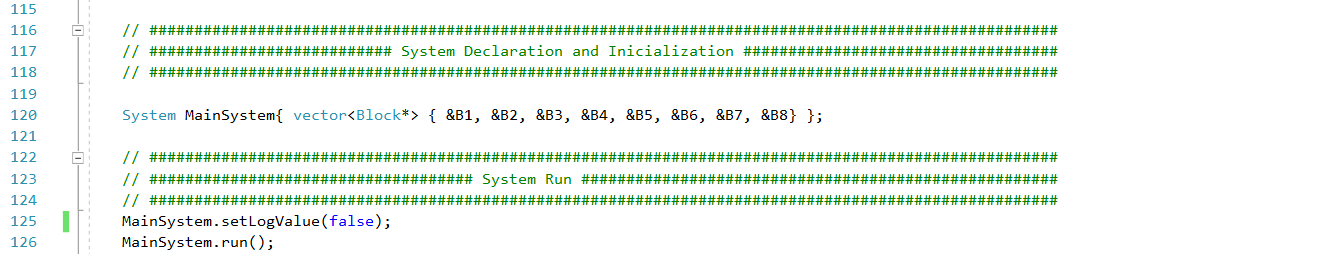
\includegraphics[width=1.3\linewidth]{./chapter/simulator_structure/figures/log_file_example}
\caption{Disabling Log File}
\label{fig:logfileexample}
\end{figure}

\subsection{Parameters}
The Log File accepts two parameters: $logFileName$ which correspond to the name of the output file, i.e., the file that will contain all the information listed above and $logValue$ which will enable the Log File if $true$ and will disable it if $false$.
\begin{table}[H]
\centering
\begin{tabulary}{1.0\textwidth}{|p{6cm}|p{4cm}|p{5cm}|}
\hline
\multicolumn{3}{|c|}{ \textbf{Log File Parameters} } \\
\hline
\textbf{Parameter}     & \textbf{Type}       & \textbf{Default Value} \\ \hline
logFileName            & string	             & "log.txt"\\ \hline
logValue               & bool	             & true\\ \hline
\end{tabulary}
\end{table}

\begin{table}[H]
\centering
\begin{tabulary}{1.0\textwidth}{|p{6cm}|p{4cm}|p{5cm}|}
\hline
\multicolumn{3}{|c|}{ \textbf{Available Set Methods} } \\
\hline
\textbf{Parameter}                    & \textbf{Type}        & \textbf{Comments} \\ \hline
setLogFileName(string newName)        & void	             & Sets the name of the output file to the name given as argument\\ \hline
setLogValue(bool value)               & void	             & Sets the value of logValue to the value given as argument\\ \hline
\end{tabulary}
\end{table}	

\subsection{Output File}
The output file will contain information about each block. From top to bottom, the output file shows the timestamp (time when the block was started), the number of samples in the buffer ready to be processed for each input signal and the signal buffer space for each output signal. This information is taken before the block has been executed. The amount of time, in seconds, that each block took to run, is also registered.
Figure \ref{fig:outputfile} shows a portion of an output file. In this example, 4 blocks have been run: MQamTransmitter, LocalOscillator, BalancedBeamSplitter and I\_HomodyneReceiver. In the case of the I\_HomodyneReceiver block we can see that the block started being ran at 23:27:37 and finished running 0.004 seconds later.

\renewcommand{\figurename}{Figure}
\begin{figure}[H]
\centering
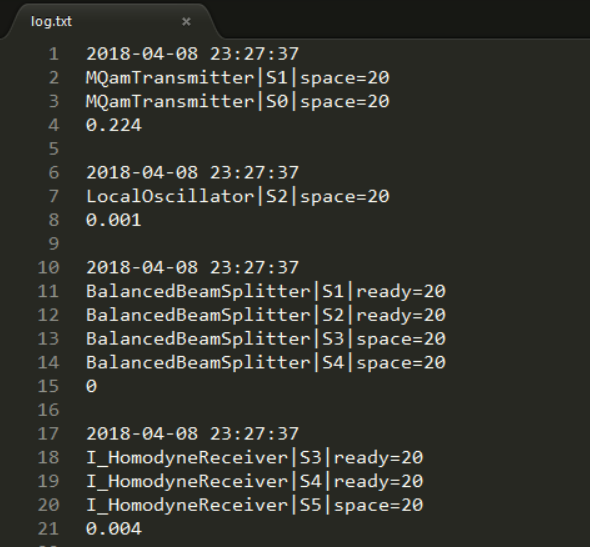
\includegraphics[width=.35\linewidth]{./chapter/simulator_structure/figures/output_file}
\caption{Output File Example}
\label{fig:outputfile}
\end{figure}

Figure \ref{fig:homodynesignals} shows a portion of code that consists in the declaration and inicialization of the I\_HomodyneReceiver block. In line 97, we can see that the block has 2 input signals, $S3$ and $S4$, and is assigned 1 output signal, $S5$. Going back to Figure \ref{fig:outputfile} we can observe that $S3$ and $S4$ have 20 samples ready to be processed and the buffer of $S5$ is empty.

\renewcommand{\figurename}{Figure}
\begin{figure}[H]
\centering
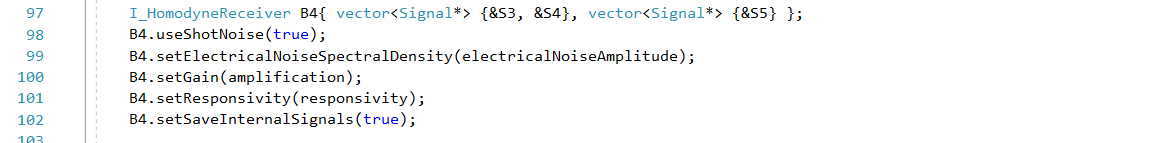
\includegraphics[width=1.3\linewidth]{./chapter/simulator_structure/figures/homodyne_signals}
\caption{I-Homodyne Receiver Block Declaration}
\label{fig:homodynesignals}
\end{figure}

The list of the input parameters loaded from a file is presented at the top of the output file, as shown in Figure \ref{fig:changedinputparameters}.

\begin{figure}[H]
\centering
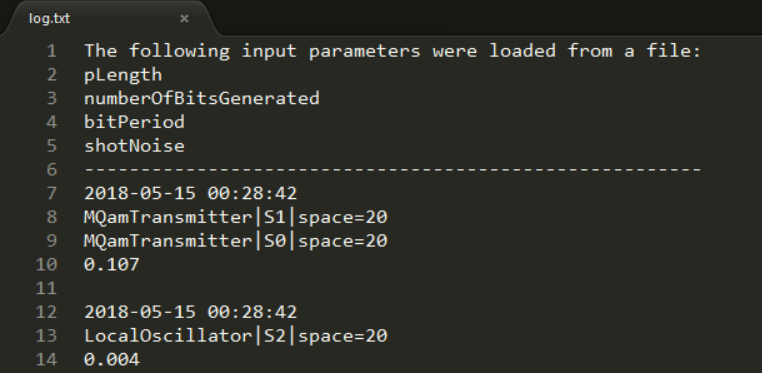
\includegraphics[width=.50\linewidth]{./chapter/simulator_structure/figures/logfile_input_parameters_changed}
\caption{Four input parameters where loaded from a file}
\label{fig:changedinputparameters}
\end{figure}

\subsection{Testing Log File}
In directory \textit{doc/tex/chapter/simulator\_structure/test\_log\_file/bpsk\_system/} there is a copy of the BPSK system. You may use it to test the Log File. The main method is located in file \textit{bpsk\_system\_sdf.cpp}

% bibliographic references for the section ----------------------------
\clearpage
\printbibliography[heading=subbibliography]
\end{refsection}
\addcontentsline{toc}{subsection}{Bibliography}
% ---------------------------------------------------------------------
\section{Input Parameters System}
\subsection{Introduction}
With the Input Parameters System (IPS) it is possible to read the input parameters from a file.

\subsubsection{Format of the Input File}
We are going to explain the use of the IPS using as an example the PBSK system.
In Figure \ref{fig:ipsfilecontent}, it is possible to observe the contents of the file \textbf{input\_parameters\_0.txt} used to load the values of some of the BPSK system's input parameters. The input file must respect the following properties:
\begin{enumerate}
\item Input parameter values can be changed by adding a line in the following format: \textbf{paramName=newValue}, where \textbf{paramName} is the name of the input parameter and \textbf{newValue} is the value to be assigned.
\item IPS supports scientific notation. This notation works for the lower case character \textbf{e} and the upper case character \textbf{E}.
\item If an input parameters is assigned the wrong type of value, method $\textbf{readSystemInputParameters()}$ will throw an exception.
\item Not all input parameters need to be changed.
\item The IPS supports comments in the form of the characters \textbf{//}. The comments will only be recognized if placed at the beginning of a line.
\end{enumerate}

\begin{figure}[H]
\centering
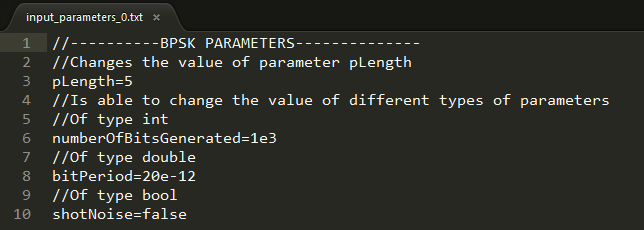
\includegraphics[width=0.8\linewidth]{./chapter/simulator_structure/figures/ips_input_file}
\caption{Content of file input\_parameters\_0.txt}
\label{fig:ipsfilecontent}
\end{figure}
\pagebreak
\subsubsection{Loading Input Parameters From A File}
Execute the following command in the Command Line:
\begin{itemize}
  \item[] \textbf{some\_system.exe <input\_file\_path> <output\_directory>}
\end{itemize}
%
where \textbf{some\_system.exe} is the name of the executable generated after compiling the project, \textbf{<input\_file\_path>} is the path to the file containing the new input parameters; \textbf{<output\_directory>} is the directory where the output signals will be written into.

\subsection{How To Include The IPS In Your System}
In this illustrative example, the code of the BPSK System will be used. To implement the IPS the following requirements must be met:
\begin{enumerate}
\item Your system must include \textbf{netxpto\_20180418.h} or later.
\item A class that will contain the system input parameters must be created. This class must be a derived class of \textbf{SystemInputParameters}. In this case the created class is called \textbf{BPSKInputParameters}.
\item The created class must have 2 constructors. The implementation of these constructors is the same as \textbf{BPSKInputParameters}.
\begin{lstlisting}
BPSKInputParameters();
BPSKInputParameters(int argc, char*argv[]);
\end{lstlisting}
\item The created class must contain the method \textbf{initializeInputParameterMap()}. For every input parameter \textbf{addInputParameter(paramName,paramAddress)} must be called, where \textbf{paramName} is a string that represents the name of your input parameter and \textbf{paramAddress} is the address of your input parameter.
\begin{lstlisting}
void initializeInputParameterMap(){
	//Add parameters
}
\end{lstlisting}
\item All signals must be instantiated using the constructor that takes as argument, the file name and the folder name, according to the type of signal.
\begin{lstlisting}
Binary S0("S0.sgn", param.getOutputFolderName()) //S0 is a Binary signal
\end{lstlisting}
\item Method \textbf{main} must receive the following arguments.
\begin{lstlisting}
int main(int argc, char*argv[]){...}
\end{lstlisting}
\item The MainSystem must be instantiated using the following line of code. The \dots represent the list of blocks.
\begin{lstlisting}
System MainSystem{ vector<Block*> {...},param.getOutputFolderName(),param.getLoadedInputParameters()};
\end{lstlisting}
\end{enumerate}
\
The following code represents the input parameters class, \textbf{BPSKInputParameters}, and must be changed according to the system you are working on.
%%%%%%%%%%%%%%%%%%%%%%%%%%%CODE%%%%%%%%%%%%%%%%%%%%%%%%%%%%%%%%
\begin{lstlisting}
class BPSKInputParameters : public SystemInputParameters {
public:
	//INPUT PARAMETERS
	int numberOfBitsReceived{ -1 };
	int numberOfBitsGenerated{ 1000 };
	int samplesPerSymbol = 16;
    (...)

	/* Initializes default input parameters */
	BPSKInputParameters() : SystemInputParameters() {
		initializeInputParameterMap();
	}

	/* Initializes input parameters according to the program arguments */
    /* Usage: .\bpsk_system.exe <input_parameters.txt> <output_directory> */
	BPSKInputParameters(int argc, char*argv[]) : SystemInputParameters(argc,argv) {
		initializeInputParameterMap();
		readSystemInputParameters();
	}

	//Each parameter must be added to the parameter map by calling addInputParameter(string,param*)
	void initializeInputParameterMap(){
		addInputParameter("numberOfBitsReceived", &numberOfBitsReceived);
		addInputParameter("numberOfBitsGenerated", &numberOfBitsGenerated);
		addInputParameter("samplesPerSymbol", &samplesPerSymbol);
        (...)
	}
};
\end{lstlisting}
The method \textbf{main} should look similar to the following code.
\begin{lstlisting}
int main(int argc, char*argv[]){

    BPSKInputParameters param(argc, argv);

    //Signal Declaration and Initialization
    Binary S0("S0.sgn", param.getOutputFolderName());
	S0.setBufferLength(param.bufferLength);

	OpticalSignal S1("S1.sgn", param.getOutputFolderName());
	S1.setBufferLength(param.bufferLength);
    (...)

    //System Declaration and Initialization
	System MainSystem{ vector<Block*> { &B1, &B2, &B3, &B4, &B5, &B6, &B7, &B8},param.getOutputFolderName(),param.getLoadedInputParameters()};

    //System Run
	MainSystem.run();

	return 0;
}
\end{lstlisting}
%%%%%%%%%%%%%%%%%%%%%%%%%%%%%%%%%%%%%%%%%%%%%%%%%%%%%%%%%%%%%%%%%%%%%%
\pagebreak
The class \textbf{SystemInputParameters}, has the following constructors and methods available:
\begin{table}[H]
\centering
\begin{tabulary}{1.0\textwidth}{|p{5cm}|p{10cm}|}
\hline
\multicolumn{2}{|c|}{ \textbf{SystemInputParameters - Constructors} } \\
\hline
\textbf{Constructors}                   & \textbf{Comments} \\ \hline
SystemInputParameters()                        & Creates an object of SystemInputParameters with the default input parameters' values\\ \hline
SystemInputParameters(int argc, char*argv[])   & Creates an object of SystemInputParameters and loads the values according to the program arguments passed in the command line\\ \hline
\end{tabulary}
\end{table}

\begin{table}[H]
\centering
\begin{tabulary}{1.0\textwidth}{|p{9cm}|p{1cm}|p{5cm}|}
\hline
\multicolumn{3}{|c|}{ \textbf{SystemInputParameters - Methods} } \\
\hline
\textbf{Method}                                      & \textbf{Type} & \textbf{Comments} \\ \hline
addInputParameter(string name, int* variable)        & void          & Adds an input parameter whose value is of type int\\ \hline
addInputParameter(string name, double* variable)     & void	         & Adds an input parameter whose value is of type double\\ \hline
addInputParameter(string name, bool* variable)       & void	         & Adds an input parameter whose value is of type bool\\ \hline
readSystemInputParameters()                          & void	         & Reads the input parameters from a file.\\ \hline
\end{tabulary}
\end{table}

\section{Documentation}

As in any large software system documentation it is critical.
The documentation is going to be developed in Latex using WinEdt as the recommend editor.
The bibliography is per section, for this to work replace the bibtex by biber, go to the WinEdt Options->Execution Modes->Bibtex and replace bibtex.exe by biber.exe.

\cleardoublepage 

%
% ------------------------------------------------------------------------
\chapter{Development Cycle}

The NetXPTO-LinkPlanner is a open source project with its core implemented using ISO C++.
At the present the followed standard is the ISO C++14.


The developed environment has been the Visual Studio Community 2017, namely release 15.5 and beyond.
The Git has been used as the version control system.
The NetXPTO-LinkPlanner repository is located in the GitHub site http://github.com/netxpto/linkplanner.
Master branch should be considered a functional beta version of the software.
Periodically new releases are delivered from the master branch under the branch name R<Release Year>-<Release Number>.
The design and integration of the system has been performed by Prof. Armando Pinto.





%\include{chapter/visualizer}
%
% ------------------------------------------------------------------------
\chapter{Case Studies}

\ifdefined\qpsk         	\section{QPSK Transmitter}

This system simulates a QPSK transmitter. A schematic representation of this system is shown in figure \ref{QPSK_transmitter_block_diagram_simple}.

\begin{figure}[h]
	\centering
	\includegraphics[width=0.5\textwidth]{figures/qpsk_transmitter.pdf}
	\caption{QPSK transmitter block diagram}\label{QPSK_transmitter_block_diagram_simple}
\end{figure}

\subsection*{Functional description}

This block generates an optical signal (output signal 1 in figure \ref{MQAM_transmitter_block_diagram}). The binary signal generated in the internal block Binary Source (block B1 in figure \ref{MQAM_transmitter_block_diagram}) can be used to perform a Bit Error Rate (BER) measurement and in that sense it works as an extra output signal (output signal 2 in figure \ref{MQAM_transmitter_block_diagram}).

\begin{figure}[h]
	\centering
	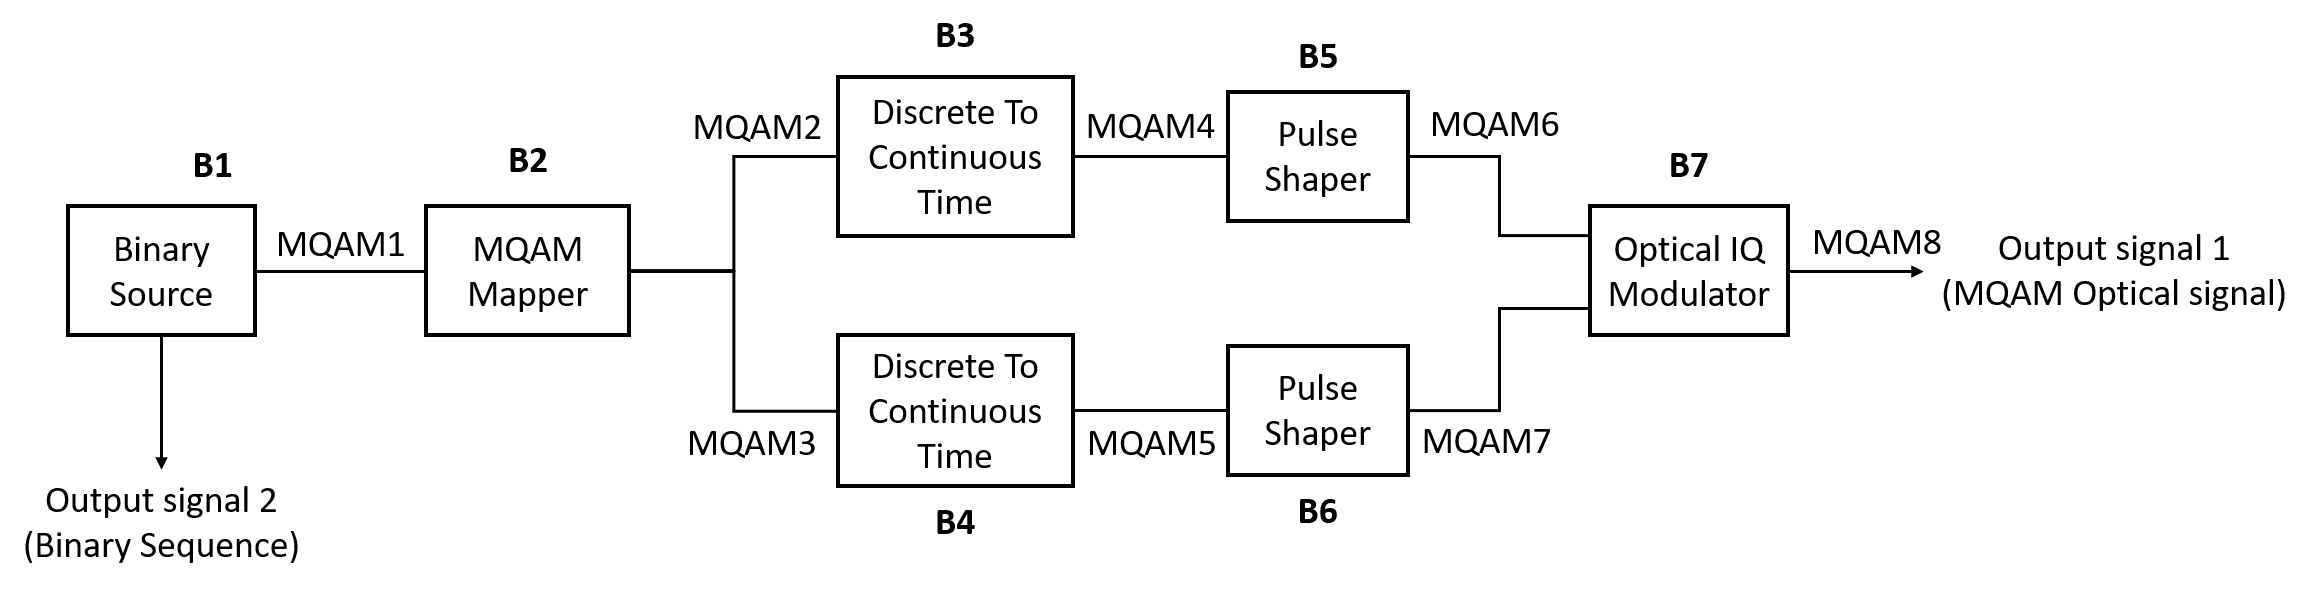
\includegraphics[width=\textwidth]{figures/MQAM_transmitter_block_diagram}
	\caption{Schematic representation of the block MQAM transmitter.}\label{MQAM_transmitter_block_diagram}
\end{figure}

\subsection*{Input parameters}

This block has a special set of functions that allow the user to change the basic configuration of the transmitter. The list of input parameters, functions used to change them and the values that each one can take are summarized in table \ref{table}.

\begin{table}[h]
\begin{center}
	\begin{tabular}{| m{3,5cm} | m{5,1cm} |  m{2,5cm} | m{4cm} | }
		\hline
		\textbf{Input parameters} & \textbf{Function} & Type & \textbf{Accepted values} \\ \hline
		Mode & setMode() & string & PseudoRandom \newline Random \newline DeterministicAppendZeros \newline DeterministicCyclic \\ \hline
		Number of bits generated & setNumberOfBits() & int & Any integer\\ \hline
		Pattern length & setPatternLength() & int & Real number greater than zero\\ \hline
		Number of bits & setNumberOfBits() & long & Integer number greater than zero\\ \hline
		Number of samples per symbol & setNumberOfSamplesPerSymbol() & int & Integer number of the type $2^n$ with n also integer\\ \hline
		Roll of factor & setRollOfFactor() & double & $\in$ [0,1] \\ \hline
		IQ amplitudes & setIqAmplitudes() & Vector of coordinate points in the I-Q plane & \textbf{Example} for a 4-qam mapping: \{ \{ 1.0, 1.0 \}, \{ -1.0, 1.0 \}, \{ -1.0, -1.0 \}, \{ 1.0, -1.0 \} \} \\ \hline
		Output optical power & setOutputOpticalPower() & int & Real number greater than zero\\ \hline
		Save internal signals & setSaveInternalSignals() & bool & True or False\\
		\hline
	\end{tabular}
	\caption{List of input parameters of the block MQAM transmitter} \label{table}
\end{center}
\end{table}

%\begin{itemize}
%	\item setMode(PseudoRandom);
%	\item setBitPeriod(1.0/50e9);
%	\linebreak (double)
%	\item setPatternLength(3);
%	\linebreak (int)
%	\item setNumberOfBits(10000);
%	\linebreak (long)
%	\item setNumberOfSamplesPerSymbol(32);
%	\linebreak (int)
%	\item setRollOffFactor(0.9);
%	\linebreak (double $\in$ [0,1])
%	\item setIqAmplitudes(\{ \{ 1, 1 \}, \{ -1, 1 \}, \{ -1, -1 \}, \{ 1, -1 \} \});
%	\item setOutputOpticalPower\_dBm(0);
%	\item setSaveInternalSignals(true);
%\end{itemize}

\pagebreak

\subsection*{Methods}

MQamTransmitter(vector$<$Signal *$>$ \&inputSignal, vector$<$Signal *$>$ \&outputSignal); (\textbf{constructor})
\bigbreak

void set(int opt);
\bigbreak
void setMode(BinarySourceMode m)
\bigbreak
BinarySourceMode const getMode(void)
\bigbreak
void setProbabilityOfZero(double pZero)
\bigbreak
double const getProbabilityOfZero(void)
\bigbreak
void setBitStream(string bStream)
\bigbreak
string const getBitStream(void)
\bigbreak
void setNumberOfBits(long int nOfBits)
\bigbreak
long int const getNumberOfBits(void)
\bigbreak
void setPatternLength(int pLength)
\bigbreak
int const getPatternLength(void)
\bigbreak
void setBitPeriod(double bPeriod)
\bigbreak
double const getBitPeriod(void)
\bigbreak
void setM(int mValue)
int const getM(void)
\bigbreak
void setIqAmplitudes(vector$<$t\textunderscore iqValues$>$ iqAmplitudesValues)
\bigbreak
vector$<$t\textunderscore iqValues$>$ const getIqAmplitudes(void)
\bigbreak
void setNumberOfSamplesPerSymbol(int n)
\bigbreak
int const getNumberOfSamplesPerSymbol(void)
\bigbreak
void setRollOffFactor(double rOffFactor)
\bigbreak
double const getRollOffFactor(void)
\bigbreak
void setSeeBeginningOfImpulseResponse(bool sBeginningOfImpulseResponse)
\bigbreak
double const getSeeBeginningOfImpulseResponse(void)
\bigbreak
void setOutputOpticalPower(t\textunderscore real outOpticalPower)
\bigbreak
t\textunderscore real const getOutputOpticalPower(void)
\bigbreak
void setOutputOpticalPower\_dBm(t\_real outOpticalPower\_dBm)
\bigbreak
t\_real const getOutputOpticalPower\_dBm(void)
\pagebreak

\subsection*{Output Signals}

\subparagraph*{Number:} 1 optical and 1 binary (optional)

\subparagraph*{Type:} Optical signal

\subsection*{Example}

\begin{figure}[h]
	\centering
	\includegraphics[width=0.8\textwidth]{figures/BinarySource_output}
	\caption{Example of the binary sequence generated by this block for a sequence 0100...}
\end{figure}

\begin{figure}[h]
	\centering
	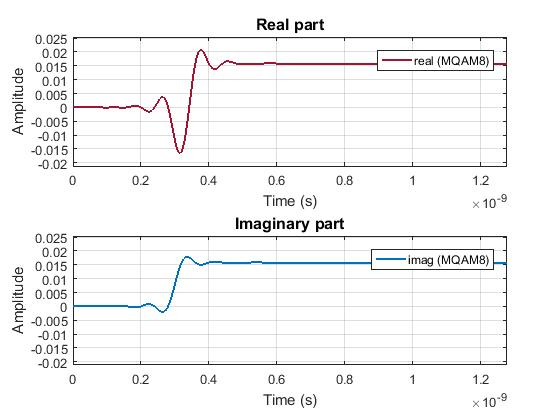
\includegraphics[width=0.8\textwidth]{figures/IQmodulator0_output}
	\caption{Example of the output optical signal generated by this block for a sequence 0100...}
\end{figure}

\subsection*{Sugestions for future improvement}

Add to the system another block similar to this one in order to generate two optical signals with perpendicular polarizations. This would allow to combine the two optical signals and generate an optical signal with any type of polarization.
 \fi
\ifdefined\optical      	\input{./sdf/optical_detection/optical_detection} \fi
\ifdefined\bpsk         	\input{./sdf/bpsk_system/bpsk_system} \fi
\ifdefined\hammingED        \clearpage
\section{Hamming Channel Encoder and Decoder }

\begin{refsection}

\begin{tcolorbox}	
	\begin{tabular}{p{2.75cm} p{0.2cm} p{10.5cm}} 	
		\textbf{Students Name} &:& Lu\'{i}s Almeida (08/06/2018 - 10/07/2018) \\
		\textbf{Goal}          &:& Implement a channel coder and decoder based on the Hamming algorithm.
	\end{tabular}
\end{tcolorbox}

Hamming Channel Encoder/Decoder simulates a channel encoder and decoder that uses the Hamming Algorithm. The goal is to perform the encoding of supplied source data, then encode it using the Hamming Encoder, pass the encoded data through a channel that implements errors according to a defined probability and finally perform the decoding using the Hamming Decoder. In the end a BER is performed to detect the possibility of errors.

\subsection{Introduction}

The Hamming code is a linear block code, was developed by Richard Hamming, is used in signal processing and telecommunications. Its use allows the transfer and storage of data in a safe and efficient way.

In telecommunications the Hamming codes used are generalizations of Hamming Code (7,4). These can detect errors up to two bits and correct up to one bit. In contrast, the parity code cannot fix errors, and can only detect an odd number of errors. Due to its simplicity the Hamming codes are widely used in computer memory (ECC). In this context, it is common to use an extended Hamming code with an extra parity bit.

In mathematical terms, Hamming codes are a class of binary linear codes. For each integer $r \geq 2$ there is a block length $n = 2^{r} -1$ and message length $k = 2^{r} - r - 1$. Therefore, the Hamming code rate is $R = k / n = 1 - r / (2^{r}r - 1)$, which is as high as possible for codes with distance $3$ and block length $2^{r} - 1$. The parity matrix of a Hamming code is constructed by listing all columns of length $r$ that are linearly independent. Hamming codes are special because they are perfect codes, that is, they reach the highest rate for the codes with their block length and a minimum distance of $3$ \cite{venkatesanguruswami2010}.

\subsection{Theoretical Analysis}

One of the most used Hamming Codes is the (7, 4), that encodes 4 data bits into 7 bit block (3 extra parity bits). The extra 3 bits will enable the receiver to detect up to 2 errors and correct one of them.

In order to encode a block of 4 data bits it is required to have a generator matrix $G$. Multiplying $[d1 ~ d2 ~ d3 ~ d4] \times G(d)]$ will result in the desired $1 \times 7$ encoded word.

The $G$ matrix can be defined for the Hamming Code $(7, 4)$ as follows:

\begin{equation}
G = [p | d];
\end{equation}

where,

\begin{equation}
	p = \begin{bmatrix}
	0 & 1 & 1 \\
	1 & 0 & 1 \\
	1 & 1 & 0 \\
	1 & 1 & 1
	\end{bmatrix}
\end{equation}

\begin{equation}
	d = \begin{bmatrix}
	1 & 0 & 0 & 0 \\
	0 & 1 & 0 & 0 \\
	0 & 0 & 1 & 0 \\
	0 & 0 & 0 & 1
	\end{bmatrix}
\end{equation}

Also for decode it is required to create a decoding matrix $H$, and using the same example Hamming Code $(7, 4)$, we can form the $H$ matrix as follows.

\begin{equation}
H = \begin{bmatrix}
1 & 0 & 0 & 0 & 1 & 1 & 1 \\
0 & 1 & 0 & 1 & 0 & 1 & 1 \\
0 & 0 & 1 & 1 & 1 & 0 & 1
\end{bmatrix}
\end{equation}

Using the $H$ matrix we can detect the presence of errors in the received 7 bit block. If we multiply $H$ by the 7 bit block the outcome will be a $3 \times 1$ vector $(err)$ that if the sum of it's values is different than zero it means an error was detected.

So to correct that error, we just need to compare the $(err)$ with the $H$ matrix and search for the column that is equal to the obtained $err$ vector. That indicates the bit that was received wrongly. To correct it, we just need to change the corresponding bit value.

After that to perform the decoding we just need to segment the last 4 bits from the 7 bit vector in order to recover the 4 data bits sent.

\subsection{Simulation Analysis}

The project flow can be observed in Figure \ref{fig:hammingEncoderDecoder}.

\begin{figure}[h!]
	\vspace{-3mm}
	\centering
	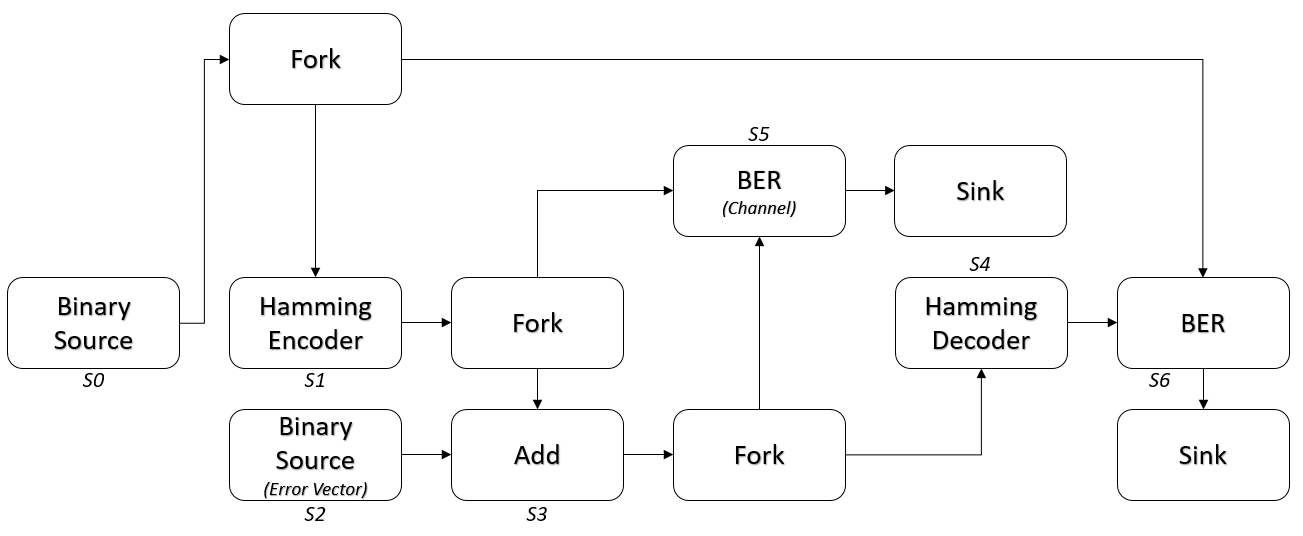
\includegraphics[width=.9\linewidth]{./sdf/eit_25828_hamming_channel_encoder_decoder/images/blockDesign.png}
	\vspace{-3mm}
	\caption{Hamming Encoder/Decoder Design Flow}
	\label{fig:hammingEncoderDecoder}
	\vspace{-3mm}
\end{figure}

Initially the project uses a Binary Source block in order to create a random number of bits that form the Data Signal $S0$ (Figure \ref{fig:hammingEncoderDecoder_S0}).

\begin{figure}[h!]
	\centering
	\includegraphics[width=.9\linewidth]{./sdf/eit_25828_hamming_channel_encoder_decoder/images/S0.png}
	\vspace{-3mm}
	\caption{S0 Signal Example for Hamming Code (7, 4)}
	\label{fig:hammingEncoderDecoder_S0}
\end{figure}

Next the $S0$ is feed into a Fork block in order to create a copy of the original signal, $S0$, so it can be feed into the following processing chain and into the BER block.

After that $S0$ is encoded using the Hamming Encoder Block and we obtain the encoded signal $S1$, according to the selected Hamming Code $(n, k)$ (Figure \ref{fig:hammingEncoderDecoder_S1}).

\begin{figure}[h!]
	\centering
	\includegraphics[width=.9\linewidth]{./sdf/eit_25828_hamming_channel_encoder_decoder/images/S1.png}
	\vspace{-3mm}
	\caption{S1 Signal Example for Hamming Code (7, 4)}
	\label{fig:hammingEncoderDecoder_S1}
\end{figure}

In order to simulate the occurrence of errors a second Binary Source block is used to generate the noise signal, $S2$, that basically produces a one accordingly to a given percentage, where it represents an error (Figure \ref{fig:hammingEncoderDecoder_S2}).

\begin{figure}[h!]
	\centering
	\includegraphics[width=.9\linewidth]{./sdf/eit_25828_hamming_channel_encoder_decoder/images/S2.png}
	\vspace{-3mm}
	\caption{S2 Signal Example for Hamming Code (7, 4)}
	\label{fig:hammingEncoderDecoder_S2}
\end{figure}

\vspace{60mm}

After that the data signal, $S0$, is summed, using an add block, with the noise signal, $S2$, and we obtain the data signal with errors, $S3$, simulating a noise channel (Figure \ref{fig:hammingEncoderDecoder_S3} and Figure \ref{fig:hammingEncoderDecoder_S1_S3}).

\begin{figure}[h!]
	\centering
	\includegraphics[width=.9\linewidth]{./sdf/eit_25828_hamming_channel_encoder_decoder/images/S3.png}
	\vspace{-3mm}
	\caption{S3 Signal Example for Hamming Code (7, 4)}
	\label{fig:hammingEncoderDecoder_S3}
\end{figure}

\begin{figure}[h!]
	\centering
	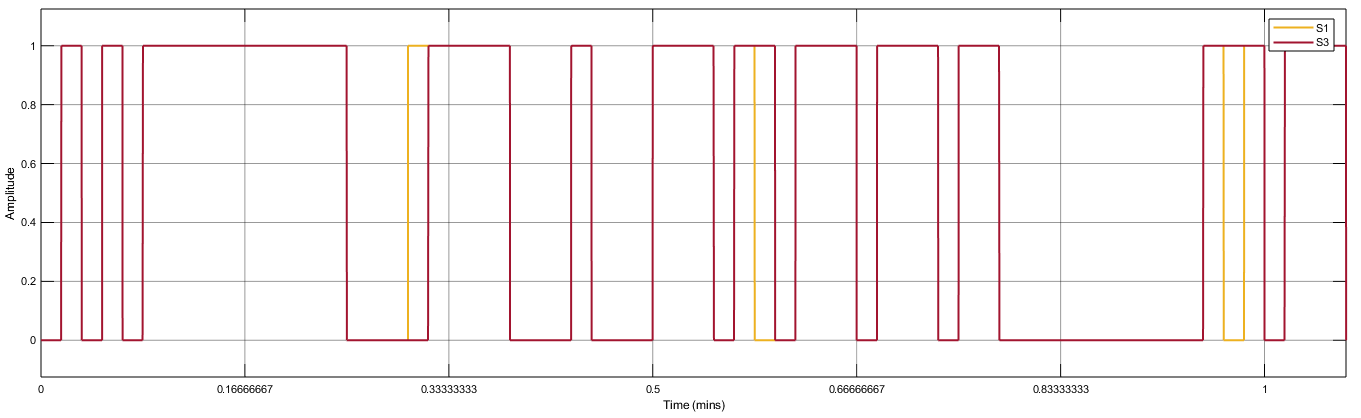
\includegraphics[width=.9\linewidth]{./sdf/eit_25828_hamming_channel_encoder_decoder/images/S1_S3.png}
	\vspace{-3mm}
	\caption{Comparison of S1 and S3 Signals}
	\label{fig:hammingEncoderDecoder_S1_S3}
\end{figure}

Then the obtained signal is decoded using the Hamming Decoder block, returning the decoded signal, $S4$ (Figure \ref{fig:hammingEncoderDecoder_S4}).

\begin{figure}[h!]
	\centering
	\includegraphics[width=.9\linewidth]{./sdf/eit_25828_hamming_channel_encoder_decoder/images/S4.png}
	\vspace{-3mm}
	\caption{S4 Signal Example for Hamming Code (7, 4)}
	\label{fig:hammingEncoderDecoder_S4}
\end{figure}

Finally a BER comparison using the BER block is performed in order to evaluate the encoding and decoding chain (Figure \ref{fig:hammingEncoderDecoder_S0_S4}).

\begin{figure}[h!]
	\centering
	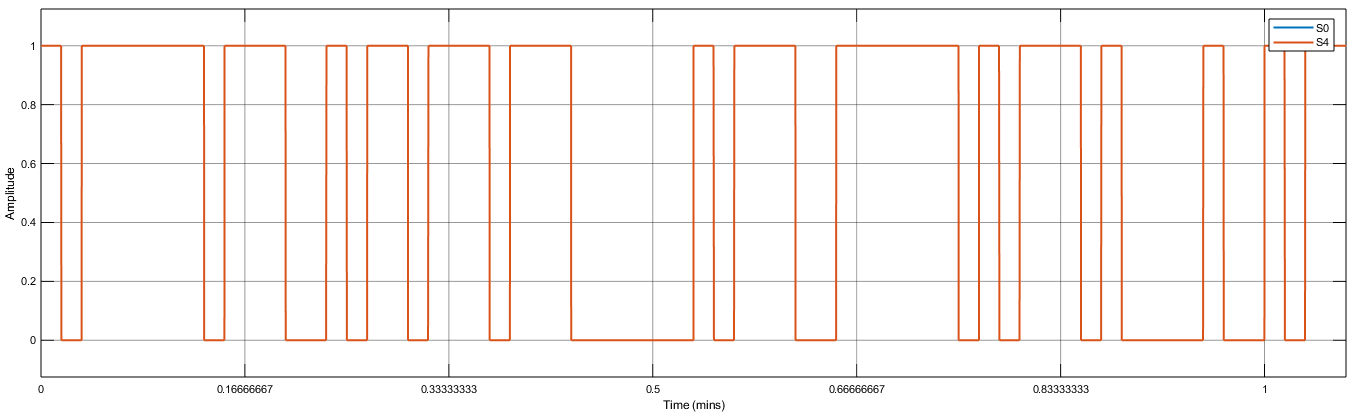
\includegraphics[width=.9\linewidth]{./sdf/eit_25828_hamming_channel_encoder_decoder/images/S0_S4.png}
	\vspace{-3mm}
	\caption{Comparison of S0 and S4 Signals (Original and Decoded Signals)}
	\label{fig:hammingEncoderDecoder_S0_S4}
	\vspace{-3mm}
\end{figure}

\vspace{-3mm}

\subsection*{BER Comparison}

\vspace{-1mm}

In this subsection we show the observed BER relations between the inputed error probability in the channel and the actual BER on the output of the channel (Figure \ref{fig:hammingEncoderDecoder_BER_input_output_channel}) and the relation between the inputed probability of error of the channel and the BER on the output of the Hamming Decoder (Figure \ref{fig:hammingEncoderDecoder_BER_input_output}) .

\begin{figure}[h!]
	\vspace{-4mm}
	\centering
	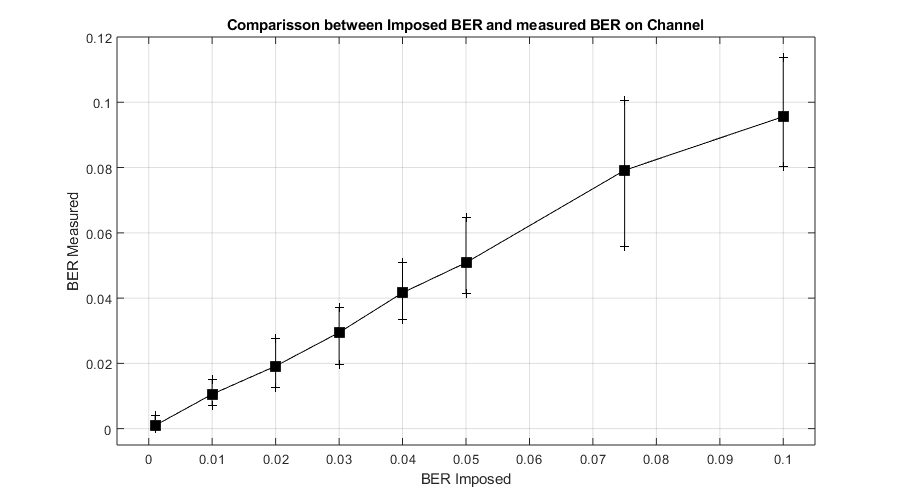
\includegraphics[width=.9\linewidth]{./sdf/eit_25828_hamming_channel_encoder_decoder/images/BER_1.png}
	\vspace{-5mm}
	\caption{Comparison between Imposed BER and measured BER on Channel}
	\label{fig:hammingEncoderDecoder_BER_input_output_channel}
\end{figure}

\begin{figure}[h!]
	\vspace{-9mm}
	\centering
	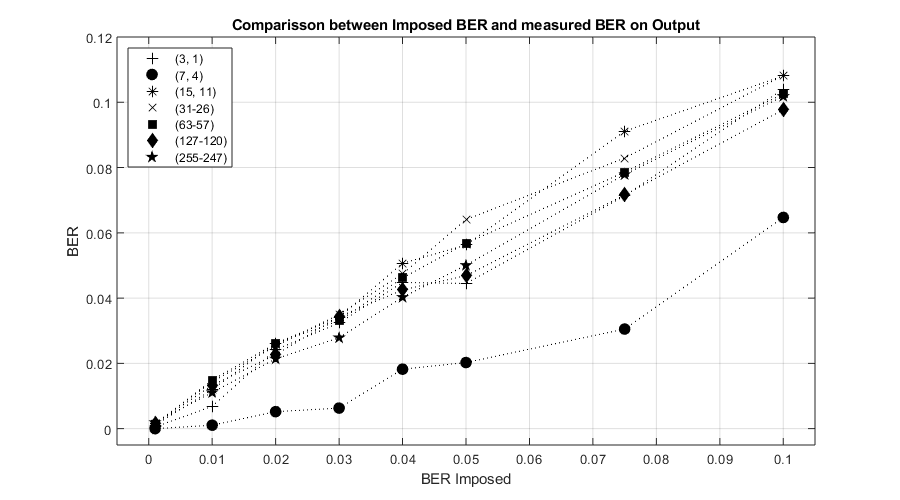
\includegraphics[width=.9\linewidth]{./sdf/eit_25828_hamming_channel_encoder_decoder/images/BER_2.png}
	\vspace{-5mm}
	\caption{Comparison between Imposed BER and measured BER on Output of Decoder}
	\label{fig:hammingEncoderDecoder_BER_input_output}
	\vspace{-30mm}
\end{figure}

\subsection*{Required files}
\label{Required files}

This project is composed by the header and source files described in following tables.

\begin{table}[H]
\centering
\begin{tabulary}{1.0\textwidth}{|p{7.5cm}|p{6.5cm}|p{1cm}|}
\hline
\multicolumn{3}{|c|}{ \textbf{Header Files} } \\
\hline
\textbf{File}                & \textbf{Comments} & \textbf{Status} \\ \hline
add\_20180620.h              &                   & \checkmark \\ \hline
binary\_source\_20180523.h   &                   & \checkmark \\ \hline
bit\_error\_rate\_20180424.h &                   & \checkmark \\ \hline
fork\_20180112.h             &                   & \checkmark \\ \hline
hamming\_coder\_20180608.h   &                   & \checkmark \\ \hline
hamming\_decoder\_20180608.h &                   & \checkmark \\ \hline
netxpto\_20180418.h          &                   & \checkmark \\ \hline
sink\_20180118.h             &                   & \checkmark \\ \hline

\end{tabulary}
\end{table}		
%
\begin{table}[H]
\centering
\begin{tabulary}{1.0\textwidth}{|p{9.5cm}|p{4.5cm}|p{1cm}|}
\hline
\multicolumn{3}{|c|}{ \textbf{Source Files} } \\
\hline
\textbf{File}              					  	   & \textbf{Comments} & \textbf{Status} \\ \hline
add\_20180620.cpp            				  	   &                   & \checkmark \\ \hline
binary\_source\_20180523.cpp   				  	   &                   & \checkmark \\ \hline
bit\_error\_rate\_20180424.cpp  				   &                   & \checkmark \\ \hline
fork\_20180112.cpp            				  	   &                   & \checkmark \\ \hline
hamming\_coder\_20180608.cpp   				  	   &                   & \checkmark \\ \hline
hamming\_decoder\_20180608.cpp 				  	   &                   & \checkmark \\ \hline
netxpto\_20180418.cpp         				  	   &                   & \checkmark \\ \hline
sink\_20180118.cpp            				  	   &                   & \checkmark \\ \hline
eit\_25828\_hamming\_channel\_encoder\_decoder.cpp &                   & \checkmark \\ \hline
\end{tabulary}
\end{table}		

\subsection*{System Input Parameters}

In order to successfully run this project it is required to set the following input parameters:

\begin{itemize}
	\item \textit{probalilityOfZero\_ErrorVector} $(p_{0})$ - Defines the probability for introducing errors (in order to simulate a non perfect channel). The probability of an error is $p_{1} = 1 - p_{0}$.
	\item \textit{hammingCode\_nBits} $n$ - Defines the Hamming Code coded word size.
	\item \textit{hammingCode\_kBits} $k$ - Defines the Hamming Code data size.
\end{itemize}

The $n$ and $k$, form the Hamming Code $(n, k)$, and the available combination of values for each of these variables can be viewed in the Hamming Encoder/Decoder in the Library Section.

\subsection*{Inputs}

This project doesn't take any input.

\subsection*{Outputs}

This project outputs the following signals:

\begin{itemize}
	\item \textbf{\textit{S0.sgn}} - The source binary signal.
	\item \textbf{\textit{S1.sgn}} - The encoded signal using the Hamming Code $(n, k)$.
	\item \textbf{\textit{S2.sgn}} - The noise signal.
	\item \textbf{\textit{S3.sgn}} - The resulting signal of adding the encoded signal $(S1.sgn)$ with the noise signal $(S2.sgn)$.
	\item \textbf{\textit{S4.sgn}} - The decoded signal using the Hamming Code $(n, k)$.
	\item \textbf{\textit{S5.sgn}} - The BER signal on the channel.
	\item \textbf{\textit{S6.sgn}} - The BER signal after decoding.
\end{itemize}

\subsection*{Open Issues}
\label{Open Issues}

The only issue found, at the time of the construction of these blocks, was not related to the developed blocks, but regarding another block, the Binary Source (\textit{binary\_source\_20180523.h}).

The mode \textit{Random} doesn't work as intended. The block requires the user to define a probability of Zero for the output of the block, but if the output buffer becomes full on the next time the block is called again to continue producing bits, the sequence is exactly the same (Figure \ref{fig:hammingEncoderDecoder_BinarySource_ERROR}).

Observing the Figure below we can see a pattern that repeats itself over and over again instead of obtaining a completely random error vector.

\begin{figure}[h!]
	\centering
	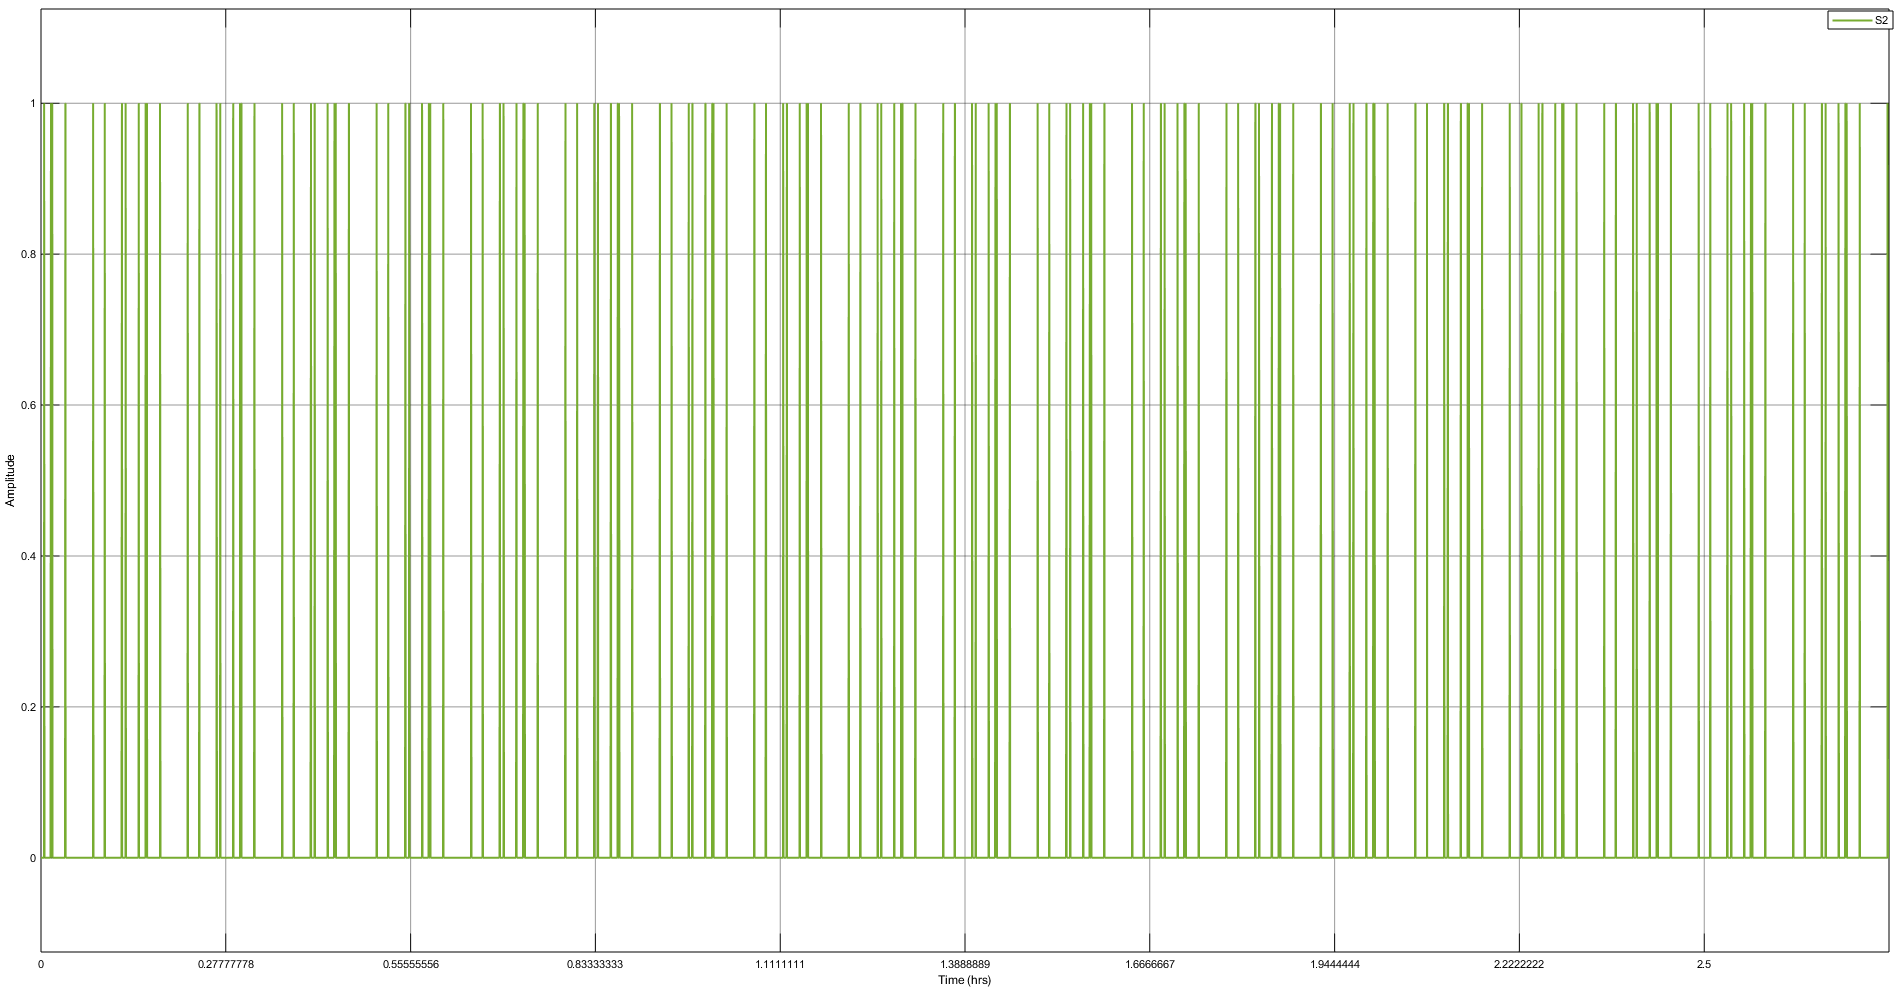
\includegraphics[width=.9\linewidth]{./sdf/eit_25828_hamming_channel_encoder_decoder/images/ERROR.png}
	\vspace{-3mm}
	\caption{Binary Source - Random mode - Observed Error}
	\label{fig:hammingEncoderDecoder_BinarySource_ERROR}
\end{figure}

\vspace{30mm}

This behavior needs to be resolved, not only to properly set this mode in the Binary Source, but also to improve the results of the developed blocks, since it is my belief that the curves observed in Figure \ref{fig:hammingEncoderDecoder_BER_input_output} would improved, reducing the BER observed on the output of the decoder for the same imposed BER.




% bibliographic references for the section ----------------------------
\clearpage
\printbibliography[heading=subbibliography]
\end{refsection}
\addcontentsline{toc}{subsection}{Bibliography}
\cleardoublepage
% --------------------------------------------------------------------- \fi
\ifdefined\huffmanED        \clearpage
\section{Huffman Source Encoder and Decoder}

\begin{refsection}

\begin{tcolorbox}	
\begin{tabular}{p{2.75cm} p{0.2cm} p{10.5cm}} 	
\textbf{Students Name}  &:& Marina Jordao (21/06/2018)\\
\textbf{Goal}          &:& Implement source code efficiency using a Huffman encoder and decoder.\\
\textbf{Directory}          &:& sdf/eit\_45550\_estimator\_source\_code\_efficiency.
\end{tabular}
\end{tcolorbox}

The main goal of this Source Code Efficiency is to estimate the code efficiency provided by a Huffman encoder. First, the source entropy is calculated and then, a Huffman encoder is implemented, in order to encode the message that was generated by a binary source.
Thereafter, the efficiency is estimated, by using entropy and message length. Lastly, a Huffman decoder is implemented in order to validate the results.
It is intend to apply this strategy for a Huffman Encoder with 2, 3 and 4 order, for a binary code with 0 and 1.


\subsection{Theoretical Analysis}


To develop an efficiency estimator several blocks were used/developed. The block diagram with the several blocks used in this project can be seen in  Figure \ref{f:RF_C}.
First, the Source block was used in order to provided the binary signal. Then, a Huffamn Encoder block was elaborated for 2, 3 and 4 orders. The efficiency estimator calculates the efficiency of the code and the Huffman Decoder will be decoded the signals for a 2,3 and 4 orders, to validade the results. The last block is the Sink, as expected.



\begin{figure}[!h]
\centering
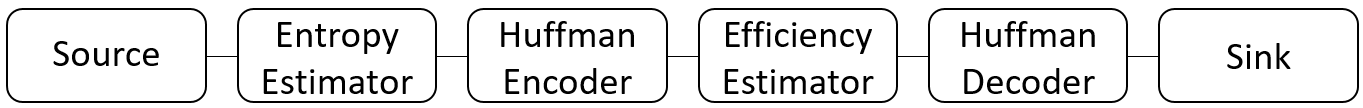
\includegraphics[width=6in]{./sdf/eit_45550_estimator_source_code_efficiency/figures/blockdiagram.png}
\caption[Block diagram of communication system]{Block diagram of source code efficiency implementation.}
\label{f:RF_C}
\end{figure}

In the following sections each block will be explained in detailed.


\subsubsection{Entropy Estimator}
In the Entropy Estimator block the main goal is to calculated the entropy from a binary source for the case of a binary source composed by 0 and 1. In this sense, to calculated the entropy the equation \ref{e:eq2} was applied.


\begin{equation}
H(x)=\sum_{i=1}^K P(a_{i})  \log_2\frac{1}{P(a_{i})}
 \label{e:eq2}
\end{equation}

This block does not have inputs variables.

\subsubsection{Hufmman Encoder}
The Hufman Encoder block aims to encode a binary signal, composed by 0 and 1, for a order of 2, 3 and 4. This block has 2 input variables, the probabilityOfZero and sourceOrder.
The probabilityOfZero variable is a double value with a range from 0 until 1. The sourceOrder variable is a integer value, where only 2, 3 and 4 values are accepted.

In this Huffman encoder, the probabilityOfZero will defined the type of codification, as well as, the source order. For a probability of zero less or equal than a probability of one, the encoder process is presented in tables \ref{tb:hufmmanencoder2}, \ref{tb:hufmmanencoder4} and \ref{tb:hufmmanencoder6}, for a source order of 2, 3 and 4 respectively.
Otherwise, if probability of zero is greater than probability of one, the encoder process is shown in tables \ref{tb:hufmmanencoder3}, \ref{tb:hufmmanencoder5} and \ref{tb:hufmmanencoder7}, for a source order of 2, 3 and 4 respectively.

\begin{table}[H]
\centering
\caption{Huffman Encoder 2 Order, when probability of Zero less or equal than probability of One}
\label{tb:hufmmanencoder2}
\begin{tabular}{|l|l|l|}
\hline
\textbf{Message}                      & \textbf{Huffman Encoder Order 2}                                       \\ \hline
00                 & 111                                                          \\ \hline
01                 & 110                                                          \\ \hline
10                 & 10                                                         \\ \hline
10                 & 0                                                         \\ \hline

\end{tabular}
\end{table}

\begin{table}[H]
\centering
\caption{Huffman Encoder 2 Order, when probability of Zero greater than probability of One}
\label{tb:hufmmanencoder3}
\begin{tabular}{|l|l|l|}
\hline
\textbf{Message}                      & \textbf{Huffman Encoder Order 2}                                       \\ \hline
11                 & 111                                                          \\ \hline
10                 & 110                                                          \\ \hline
01                 & 10                                                         \\ \hline
00                 & 0                                                         \\ \hline

\end{tabular}
\end{table}


\begin{table}[H]
\centering
\caption{Huffman Encoder 3 Order, when probability of Zero less or equal than probability of One}
\label{tb:hufmmanencoder4}
\begin{tabular}{|l|l|l|}
\hline
\textbf{Message}                      & \textbf{Huffman Encoder Order 3}                                       \\ \hline
000                 & 1111111                                                          \\ \hline
001                 & 1111110                                                          \\ \hline
010                 & 111110                                                         \\ \hline
011                 & 11110                                                   \\ \hline
100                 & 1110                                                          \\ \hline
101                 & 110                                                          \\ \hline
110                 & 10                                                         \\ \hline
111                 & 0                                                         \\ \hline
\end{tabular}
\end{table}

\begin{table}[H]
\centering
\caption{Huffman Encoder 3 Order, when probability of Zero greater than probability of One}
\label{tb:hufmmanencoder5}
\begin{tabular}{|l|l|l|}
\hline
\textbf{Message}                      & \textbf{Huffman Encoder Order 3}                                       \\ \hline
111                 & 1111111                                                          \\ \hline
110                 & 1111110                                                          \\ \hline
101                 & 111110                                                         \\ \hline
100                 & 11110                                                   \\ \hline
011                 & 1110                                                          \\ \hline
010                 & 110                                                          \\ \hline
001                 & 10                                                         \\ \hline
000                 & 0                                                         \\ \hline
\end{tabular}
\end{table}



\begin{table}[H]
\centering
\caption{Huffman Encoder 4 Order, when probability of Zero less or equal than probability of One}
\label{tb:hufmmanencoder6}
\begin{tabular}{|l|l|l|}
\hline
\textbf{Message}                      & \textbf{Huffman Encoder Order 4}                                       \\ \hline
0000                 & 111111111111111                                                         \\ \hline
0001                 & 111111111111110                                              \\ \hline
0010                 & 11111111111110                                            \\ \hline
0011                 & 1111111111110                                       \\ \hline
0100                 & 111111111110                                                          \\ \hline
0101                 & 11111111110                                                          \\ \hline
0110                 & 1111111110                                                         \\ \hline
0111                 & 111111110                                                         \\ \hline
1000                 & 11111110                                                          \\ \hline
1001                 & 1111110                                                          \\ \hline
1010                 & 111110                                                         \\ \hline
1011                 & 11110                                                   \\ \hline
1100                 & 1110                                                          \\ \hline
1101                 & 110                                                          \\ \hline
1110                 & 10                                                         \\ \hline
1111                 & 0                                                         \\ \hline
\end{tabular}
\end{table}


\begin{table}[H]
\centering
\caption{Huffman Encoder 4 Order, when probability of Zero greater than probability of One}
\label{tb:hufmmanencoder7}
\begin{tabular}{|l|l|l|}
\hline
\textbf{Message}                      & \textbf{Huffman Encoder Order 4}                                       \\ \hline
1111                 & 111111111111111                                                         \\ \hline
1110                 & 111111111111110                                              \\ \hline
1101                 & 11111111111110                                            \\ \hline
1100                 & 1111111111110                                       \\ \hline
1011                 & 111111111110                                                          \\ \hline
1010                 & 11111111110                                                          \\ \hline
1001                 & 1111111110                                                         \\ \hline
1000                 & 111111110                                                         \\ \hline
0111                 & 11111110                                                          \\ \hline
0110                 & 1111110                                                          \\ \hline
0101                 & 111110                                                         \\ \hline
0100                 & 11110                                                   \\ \hline
0011                 & 1110                                                          \\ \hline
0010                 & 110                                                          \\ \hline
0001                 & 10                                                         \\ \hline
0000                 & 0                                                         \\ \hline
\end{tabular}
\end{table}

\subsubsection{Efficiency Estimator}
The Efficiency Estimator (Source Code Efficiency) block goal is to calculate the efficiency of the code, for a order code of 2, 3 and 4. This block has 2 input variables, the probabilityOfZero and sourceOrder.
In this sense, to calculate the efficiency, the equation \ref{e:eq} was used, where L is length codeword.

\begin{equation}
\eta=\frac{Hr(x)}{L}
 \label{e:eq}
\end{equation}

\subsubsection{Hufman Decoder}


The Hufman Decoder block aims to decode signal from Huffman Encoder block, composed by 0 and 1, for a order of 2, 3 and 4. This block has 2 input variables, the probabilityOfZero and sourceOrder.
The probabilityOfZero variable is a double value with a range from 0 until 1. The sourceOrder variable is a integer value, where only 2, 3 and 4 are accepted.

In this Huffman decoder, the probabilityOfZero will defined the type of descodification, as well as, the source order. For a probability of zero less or equal than a probability of one, the decoder process is presented in tables \ref{tb:hufmmandecoder2}, \ref{tb:hufmmandecoder4} and \ref{tb:hufmmandecoder6}, for a source order of 2, 3 and 4 respectively.
Otherwise, if probability of zero is greater than probability of one, the decoder process is shown in tables \ref{tb:hufmmandecoder3}, \ref{tb:hufmmandecoder5} and \ref{tb:hufmmandecoder7}, for a source order of 2, 3 and 4 respectively.


\begin{table}[H]
\centering
\caption{Huffman Decoder 2 Order, when probability of Zero less or equal than probability of One}
\label{tb:hufmmandecoder2}
\begin{tabular}{|l|l|l|}
\hline
\textbf{Message}                      & \textbf{Huffman Decoder Order 2}                                       \\ \hline
111              & 00                                               \\ \hline
110              & 01                                           \\ \hline
10                & 10                                      \\ \hline
0                  & 11                                  \\ \hline

\end{tabular}
\end{table}

\begin{table}[H]
\centering
\caption{Huffman Decoder 2 Order, when probability of Zero greater than probability of One}
\label{tb:hufmmandecoder3}
\begin{tabular}{|l|l|l|}
\hline
\textbf{Message}                      & \textbf{Huffman Decoder Order 2}                                       \\ \hline
111         &11                                                          \\ \hline
110         &10                                                        \\ \hline
10           &01                                               \\ \hline
0             &00                                       \\ \hline

\end{tabular}
\end{table}


\begin{table}[H]
\centering
\caption{Huffman Decoder 3 Order, when probability of Zero less or equal than probability of One}
\label{tb:hufmmandecoder4}
\begin{tabular}{|l|l|l|}
\hline
\textbf{Message}                      & \textbf{Huffman Decoder Order 3}                                       \\ \hline
1111111    & 000                                                      \\ \hline
1111110    & 001                                                     \\ \hline
111110      & 010                                                   \\ \hline
11110        & 011                                          \\ \hline
1110          & 100                                               \\ \hline
110            & 101                                             \\ \hline
10              & 110                                          \\ \hline
0                & 111                                         \\ \hline
\end{tabular}
\end{table}

\begin{table}[H]
\centering
\caption{Huffman Decoder 3 Order, when probability of Zero greater than probability of One}
\label{tb:hufmmandecoder5}
\begin{tabular}{|l|l|l|}
\hline
\textbf{Message}                      & \textbf{Huffman Decoder Order 3}                                       \\ \hline
 1111111 &111                                                                           \\ \hline
1111110  &110                                                          \\ \hline
111110    &101                                                    \\ \hline
11110      &100                                              \\ \hline
1110        &011                                                  \\ \hline
110          &010                                                 \\ \hline
10            &001                                              \\ \hline
0              &000                                            \\ \hline
\end{tabular}
\end{table}



\begin{table}[H]
\centering
\caption{Huffman Decoder 4 Order, when probability of Zero less or equal than probability of One}
\label{tb:hufmmandecoder6}
\begin{tabular}{|l|l|l|}
\hline
\textbf{Message}                      & \textbf{Huffman Decoder Order 4}                                       \\ \hline
111111111111111         & 0000                                                \\ \hline
111111111111110         & 0001                                      \\ \hline
11111111111110           & 0010                                  \\ \hline
1111111111110             & 0011                          \\ \hline
111111111110               & 0100                                           \\ \hline
11111111110                 & 0101                                          \\ \hline
1111111110                   & 0110                                      \\ \hline
111111110                     & 0111                                    \\ \hline
11111110                       & 1000                                   \\ \hline
1111110                         & 1001                                 \\ \hline
111110                           & 1010                              \\ \hline
11110                             & 1011                      \\ \hline
1110                               & 1100                           \\ \hline
110                                 & 1101                         \\ \hline
10                                   & 1110                      \\ \hline
 0                                    & 1111                     \\ \hline
\end{tabular}
\end{table}


\begin{table}[H]
\centering
\caption{Huffman Decoder 4 Order, when probability of Zero greater than probability of One}
\label{tb:hufmmandecoder7}
\begin{tabular}{|l|l|l|}
\hline
\textbf{Message}                      & \textbf{Huffman Decoder Order 4}                                       \\ \hline
111111111111111      & 1111                                                   \\ \hline
111111111111110      & 1110                                        \\ \hline
11111111111110        & 1101                                    \\ \hline
1111111111110          & 1100                             \\ \hline
111111111110            & 1011                                              \\ \hline
11111111110              & 1010                                            \\ \hline
1111111110                & 1001                                         \\ \hline
111111110                  & 1000                                       \\ \hline
11111110                    & 0111                                      \\ \hline
1111110                      & 0110                                     \\ \hline
111110                        & 0101                                 \\ \hline
11110                          & 0100                         \\ \hline
1110                            & 0011                              \\ \hline
110                              & 0010                            \\ \hline
10                                & 0001                         \\ \hline
0                                  & 0000                      \\ \hline
\end{tabular}
\end{table}

In table \ref{tb:inputparameters2} are presented the input parameters of the system.





\subsection{Simulation Analysis}

The simulation implementation will be described in order to implement the Source Code Efficiency project. In Figure \ref{f:simulationdiagram} the block diagram of simulation process is shown.
For this simulation, the value of probabilityOfZero variable was 0.05.

\begin{figure}[!h]
\centering
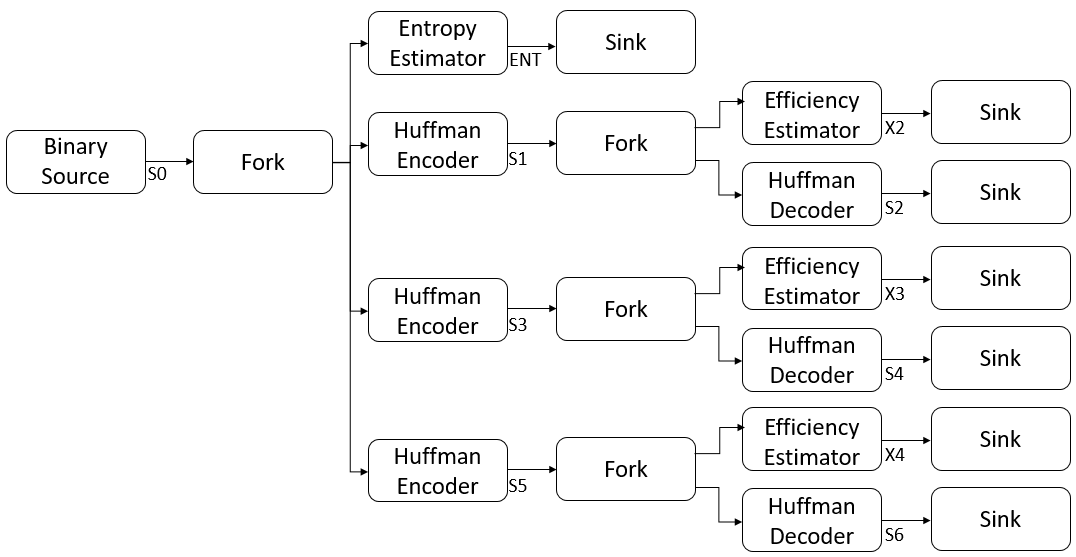
\includegraphics[width=6in]{./sdf/eit_45550_estimator_source_code_efficiency/figures/simulationdiagram.png}
\caption[Simulation Block diagram.]{Simulation Block diagram.}
\label{f:simulationdiagram}
\end{figure}

First, the Binary source block is executed, in order to generate a sequence of random binary bits, which results in the S0 signal. In Figure \ref{f:S0} can be seen an example of a S0 signal, as a result of Binary Source code.


\begin{figure}[!h]
\centering
\includegraphics[width=5in]{./sdf/eit_45550_estimator_source_code_efficiency/figures/S0.png}
\caption[S0 Signal from binary source.]{S0 Signal from binary source.}
\label{f:S0}
\end{figure}

After acquired the S0 signal, a fork was made to copy this signal. Four copies were created, one copy of this signal was applied in Entropy Estimator block, other in Huffman Encoder 2 order,  other in Huffman Encoder 3 order and the last copy was applied in Huffman Encoder 4 order.

The first copy was applied to Entropy Estimator block to estimate the entropy value of this random binary code, the resulting entropy signal from this block is shown in Figure \ref{f:entropy}. As expected, the entropy value converges to 1.
\begin{figure}[!h]
\centering
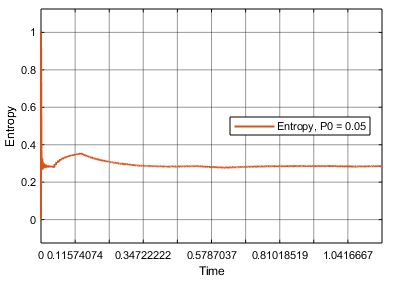
\includegraphics[width=4in]{./sdf/eit_45550_estimator_source_code_efficiency/figures/entropy.png}
\caption[Entropy results for aa binary source.]{Entropy results for a binary source.  The entropy theorical value is 0.2864.}
\label{f:entropy}
\end{figure}

The second copy was applied in the Hufman Encoder, with a source order of 2. In Figure \ref{f:S1} is presented the S1 signal, which is the result of Hufman Encoder 2 order, when the S0 signal was encoded.
Then, a fork was applied to copy the signal S1 in 2 signals, one to applied in the Efficiency Estimator block and other to applied in the Hufman Decoder block, using a source order of 2.
From the Efficiency Estimator arises the signal X2, wich can be seen in Figure \ref{f:efficiencygraph} and the decoder signal S2 from Hufman Decoder block, for a order of 2 appears in Figure \ref{f:S2}.
\begin{figure}[!h]
\centering
\includegraphics[width=5in]{./sdf/eit_45550_estimator_source_code_efficiency/figures/S1.png}
\caption[S1 Signal from Hufman Encoder 2 order.]{S1 Signal from Hufman Encoder 2 order.}
\label{f:S1}
\end{figure}


\begin{figure}[!h]
\centering
\includegraphics[width=5in]{./sdf/eit_45550_estimator_source_code_efficiency/figures/S2.png}
\caption[S2 Signal from Hufman Decoder 2 order.]{S2 Signal from Hufman Decoder 2 order.}
\label{f:S2}
\end{figure}

The third copy of signal S0 was applied in the Hufman Encoder, with a source order of 3. In Figure \ref{f:S3} is presented the S3 signal, which is the result of Hufman Encoder 3 order, when the S0 signal was encoded.
Then, a fork was applied to copy the signal S3 in 2 signals, one to applied in the Efficiency Estimator block and other to applied in the Hufman Decoder block, using a source order of 3.
From the Efficiency Estimator arises the signal X3, wich can be seen in Figure \ref{f:efficiencygraph} and the decoder signal S4 from Hufman Decoder block, for a order of 3 appears in Figure \ref{f:S4}.

\begin{figure}[!h]
\centering
\includegraphics[width=5in]{./sdf/eit_45550_estimator_source_code_efficiency/figures/S3.png}
\caption[S3 Signal from Hufman Encoder 3 order.]{S3 Signal from Hufman Encoder 3 order.}
\label{f:S3}
\end{figure}


\begin{figure}[!h]
\centering
\includegraphics[width=5in]{./sdf/eit_45550_estimator_source_code_efficiency/figures/S4.png}
\caption[S4 Signal from Hufman Decoder 3 order.]{S4 Signal from Hufman Decoder 3 order.}
\label{f:S4}
\end{figure}

The fourth copy of signal S0 was applied in the Hufman Encoder, with a source order of 4. In Figure \ref{f:S5} is presented the S5 signal, which is the result of Hufman Encoder 4 order, when the S0 signal was encoded.
Then, a fork was applied to copy the signal S5 in 2 signals, one to applied in the Efficiency Estimator block and other to applied in the Hufman Decoder block, using a source order of 4.
From the Efficiency Estimator arises the signal X4, wich can be seen in Figure \ref{f:efficiencygraph} and the decoder signal S6 from Hufman Decoder block, for a order of 4 appears in Figure \ref{f:S6}.


\begin{figure}[!h]
\centering
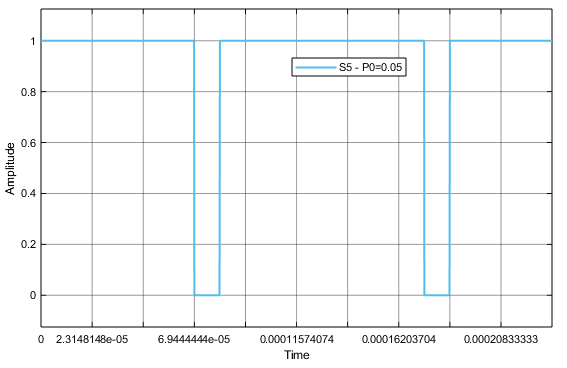
\includegraphics[width=5in]{./sdf/eit_45550_estimator_source_code_efficiency/figures/S5.png}
\caption[S5 Signal from Hufman Encoder 4 order.]{S5 Signal from Hufman Encoder 4 order.}
\label{f:S5}
\end{figure}


\begin{figure}[!h]
\centering
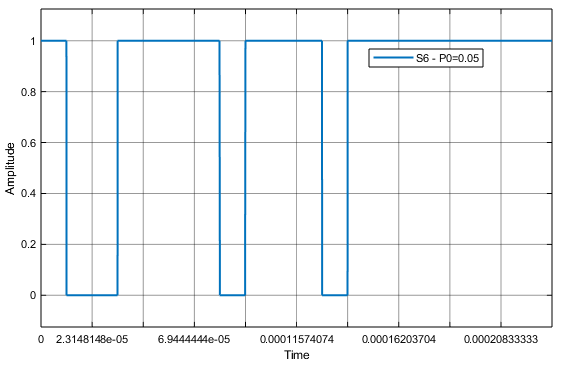
\includegraphics[width=5in]{./sdf/eit_45550_estimator_source_code_efficiency/figures/S6.png}
\caption[S6 Signal from Hufman Decoder 4 order.]{S6 Signal from Hufman Decoder 4 order.}
\label{f:S6}
\end{figure}

In order to validate that the encoder and decoder Hufman process was well developed for 2, 3 and 4 order, the original signal S0 was compared with signals S2, S4 and S6, which are the decoded signals of a source order of 2, 3 and 4 respectively.
This comparation of signals can be seen in Figure \ref{f:S0S2S4S6}. As can be seen, the signals are overlapping, which proves that the coding and decoding process were well applied.

\begin{figure}[!h]
\centering
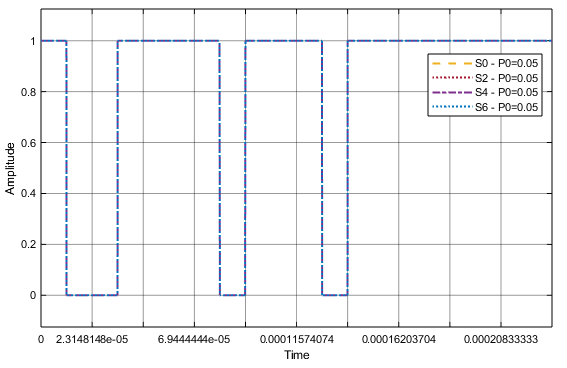
\includegraphics[width=5in]{./sdf/eit_45550_estimator_source_code_efficiency/figures/S0S2S4S6.png}
\caption[S0, S2, S4 and S6 signals comparation]{S0, S2, S4 and S6 signals comparation.}
\label{f:S0S2S4S6}
\end{figure}

In Figure \ref{f:efficiencygraph} can be seen the efficiency results for a source order of 2, 3 and 4 respectively. As expected, when the source order increases, the efficiency of the code decreases.

\begin{figure}[!h]
\centering
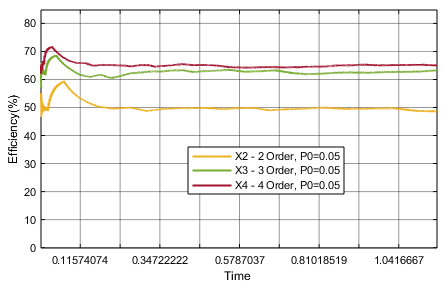
\includegraphics[width=4.2in]{./sdf/eit_45550_estimator_source_code_efficiency/figures/efficiencygraph.png}
\caption[Efficiency results for 2, 3 and 4 orders using Hufman Encoder.]{Efficiency results for 2, 3 and 4 orders using Hufman Encoder. The efficiency theorical values for each order are 49.92\%, 63.65\% and 65.46\%, respectively.}
\label{f:efficiencygraph}
\end{figure}

In the end, the sink block was used to to empty the buffer.

The project is composed by several parts. Table \ref{tb:signalsh2} shows the header files used to implement the simulation presented in Figure \ref{f:simulationdiagram}.
The source files are presented in table \ref{tb:signalss} and finally, in table \ref{tb:signals22} are shown the system signals, with the signal type information and description.
\begin{table}[H]
\centering
\caption{Header Files}
\label{tb:signalsh2}
\begin{tabular}{|c|c|c|}
\hline
\textbf{File name}                              & \textbf{Description}                                                          & \textbf{Status} \\ \hline
binary\_source\_20180523.h              &                      &    \checkmark   \\ \hline
entropy\_estimator\_20180621.h                           &                      &    \checkmark   \\ \hline
fork\_20180112.h      &                      &   \checkmark   \\ \hline
huffman\_decoder\_20180621.h                         &                      &    \checkmark   \\ \hline
huffman\_encoder\_20180621.h          &                      &    \checkmark   \\ \hline
netxpto\_20180418.h           &                      &    \checkmark   \\ \hline
sink\_20180118.h            &                      &    \checkmark   \\ \hline
source\_code\_efficiency\_20180621.h                                    &                      &    \checkmark   \\ \hline
\end{tabular}
\end{table}

\begin{table}[H]
\centering
\caption{Source Files}
\label{tb:signalss}
\begin{tabular}{|c|c|c|}
\hline
\textbf{File name}                              & \textbf{Description} & \textbf{Status} \\ \hline
binary\_source\_20180523.cpp              &                      &    \checkmark   \\ \hline
eit\_45550\_estimator\_source\_code\_efficiency\_sdf.cpp     &                      &    \checkmark   \\ \hline
entropy\_estimator\_20180621.cpp                             &                      &    \checkmark   \\ \hline
fork\_20180112.cpp      &                      &   \checkmark   \\ \hline
huffman\_decoder\_20180621.cpp                         &                      &    \checkmark   \\ \hline
huffman\_encoder\_20180621.cpp          &                      &    \checkmark   \\ \hline
netxpto\_20180418.cpp            &                      &    \checkmark   \\ \hline
sink\_20180118.cpp            &                      &    \checkmark   \\ \hline
source\_code\_efficiency\_20180621.cpp                                        &                      &    \checkmark   \\ \hline
\end{tabular}
\end{table}


\begin{table}[h]
\centering
\caption{System Signals}
\label{tb:signals22}
\begin{tabular}{|c|c|c|}
\hline
\textbf{Signal name}                            & \textbf{Signal type}         & \textbf{Description}                   \\ \hline

S0                                              &  Binary    & Binary signal which results \\
 &&from Source block\\
\hline

ENT                                              &  TimeContinuousAmplitudeContinuousReal  &  Entropy signal which results \\
 &&from Entropy Estimator block\\
\hline

S1                                              &  Binary                          & Signal encoded by Huffman\\
 && Encoder block, with order 2\\
\hline
X2                                              &  TimeContinuousAmplitudeContinuousReal   &Efficiency signal which results from                 \\
 &&Source Code Efficiency block\\
 && with order 2\\
 \hline
S2                                              &  Binary                        & Binary signal decoder by Huffman\\
 &&  Decoder block, with order 2\\
\hline
S3                                              &  Binary    &Signal encoded by Huffman\\
 && Encoder block, with order 3\\
\hline
X3                                              &  TimeContinuousAmplitudeContinuousReal &   Efficiency signal which results from                 \\
 &&Source Code Efficiency block\\
 && with order 3\\
 \hline
S4                                              &  Binary                                   & Binary signal decoder by Huffman\\
 &&  Decoder block, with order 3\\
\hline
S5                                              &  Binary    &Signal encoded by Huffman\\
 && Encoder block, with order 4\\
\hline
X4                                              &  TimeContinuousAmplitudeContinuousReal &   Efficiency signal which results from                 \\
 &&Source Code Efficiency block\\
 && with order 4\\
 \hline
S6                                              &  Binary                                   & Binary signal decoder by Huffman\\
 &&  Decoder block, with order 4\\
\hline
\end{tabular}
\end{table}

To run this simulation, different values can be applied to the probabilityOfZero variable.


% bibliographic references for the section ----------------------------
\clearpage
%\printbibliography[heading=subbibliography]
\end{refsection}
%\addcontentsline{toc}{subsection}{Bibliography}
\cleardoublepage
% --------------------------------------------------------------------- \fi
\ifdefined\arithemeticED    \clearpage
\section{Arithmetic Encoding \& Decoding}

\begin{refsection}

\begin{tcolorbox}	
\begin{tabular}{p{2.75cm} p{0.2cm} p{10.5cm}} 	
\textbf{Students Name}  &:& Diogo Barros (46084) \\
\textbf{Starting Date} &:& July 17, 2018\\
\textbf{Goal}          &:& Integer implementation of Arithmetic encoding and decoding.
\end{tabular}
\end{tcolorbox}

Arithmetic encoding is a source coding technique that represents a complete string as a real number in a sub-interval of the unit interval [0,1). Since this interval has unlimited real numbers, it is possible to assign an unique real number to any string of a given length. The coded string is the binary representation of the assigned real value.

Unlike Huffman encoding, a unique code is obtained without the need to generate all codes of all possible strings of the same length, though the implementation of arithmetic coding is significantly more complex to circumvent numeric precision problems.

\subsection{Encoding Algorithm}

\begin{tcolorbox}	
	\begin{tabular}{p{2.75cm} p{0.2cm} p{10.5cm}} 	
		\textbf{Students Name}  &:& Diogo Barros (17/07/2018 - 20/07/2018)\\
		\textbf{Goal}          &:& Arithmetic Encoding Algorithm Description
	\end{tabular}
\end{tcolorbox}

The first reference to arithmetic encoding was made in~\cite{Abramson63}. However, the first practical implementations were only proposed in 1976 by Pasco~\cite{Pasco76} and Rissanen~\cite{Rissanen76}. The block diagram of the algorithm in it's most simple floating point formulation is presented in Fig. \ref{fig:arithEncBlockDiagr}.

\begin{figure}[t]
	\centering
	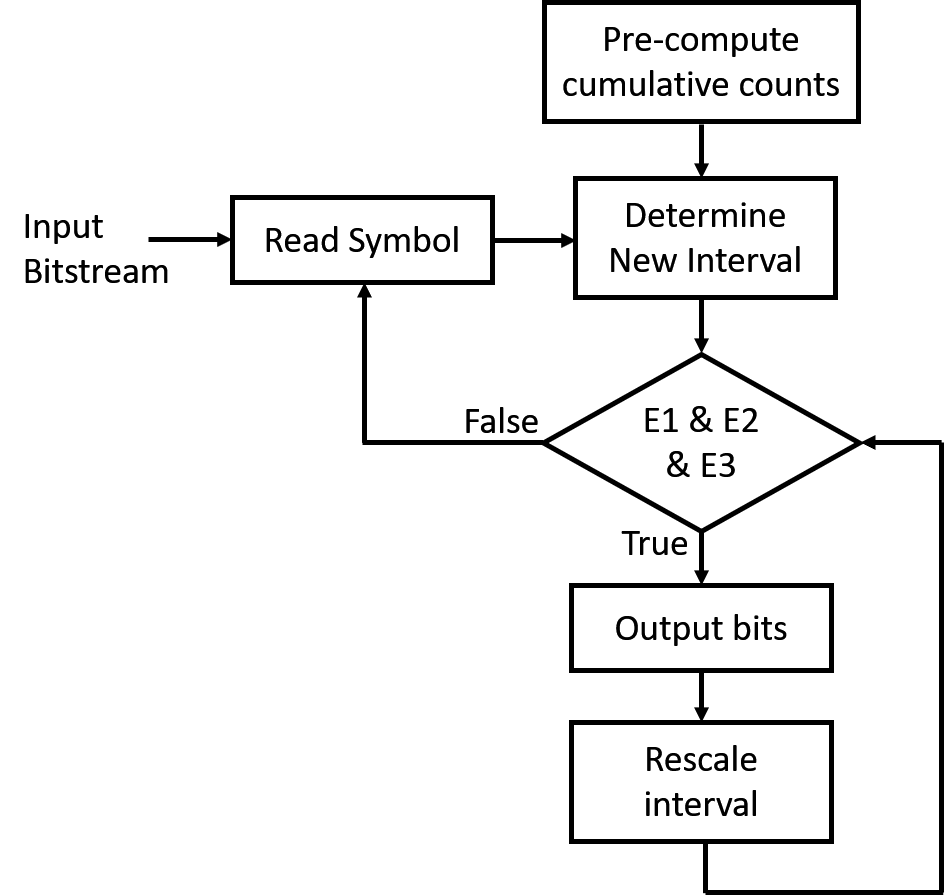
\includegraphics[width=0.6\textwidth]{./sdf/eit_46084_arithmetic_encoder_decoder/figures/ArithEncoderBlockDiagram.png}
	\caption{Block diagram of the algorithm for arithmetic encoding.} \label{fig:arithEncBlockDiagr}
\end{figure}

The first step before the encoding starts is to compute the cumulative symbol probabilities of the source, given the probabilities of each individual symbol. The initial interval is set to [0,1) and is subdivided into sub intervals based on the symbol probabilities. The required resolution (number of bits) of the registers that represent the limits of the current interval is given by the lowest symbol probability as expressed in (\ref{eq:resolEq})
\begin{equation} \label{eq:resolEq}
	Resolution = \lceil(-\log_2(\min(P(x_n))))\rceil + 1
\end{equation}

The encoding process starts by reading a symbol, identifying the corresponding sub interval in the current interval and updating the variables that save the current interval limits by using (\ref{eq:updateInterval1})-(\ref{eq:updateInterval3}).
\begin{eqnarray}
\label{eq:updateInterval1} &delta = lim\_high - lim\_low + 1 \\
&lim\_high = lim\_low + \lfloor delta \cdot count(symb + 1) / total\_count \rfloor - 1 \\
\label{eq:updateInterval3} &lim\_low = lim\_low + \lfloor delta \cdot count(symb) / total\_count \rfloor
\end{eqnarray}

At this point we need to perform two operations. The first is to check if we are able to output any code bit. The second is to rescale the interval if its amplitude is small enough. These operations are done based on the three conditions (\ref{eq:E1}), (\ref{eq:E2}) and (\ref{eq:E3}). The algorithm keeps track of how many times condition (\ref{eq:E3}) is met in succession and increments an internal extra bit counter.
\begin{eqnarray}
\label{eq:E1} &E1 = (lim\_low < 0.5) \  \&\& \ (lim\_high < 0.5) \\
\label{eq:E2} &E2 = (lim\_low > 0.5) \ \&\& \ (lim\_high > 0.5) \\
\label{eq:E3} &E3 = (lim\_low > 0.25) \ \&\& \ (lim\_high < 0.75)
\end{eqnarray}

When (\ref{eq:E1}) is met, the algorithm outputs a '0' and a number of extra '1' bits equal to the number of times (\ref{eq:E3}) was met previously and the extra bit counter is reset. When (\ref{eq:E1}) is met, the algorithm outputs a '1' and a number of '0' bits equal to the number of times (\ref{eq:E3}) was met previously and the extra bit counter is reset. In the practical implementation, these conditions are tested by comparing the most significant bits of each register.

If any of these conditions is met, the amplitude of the interval is lower than $0.25$ and needs to be rescaled by a factor of two, depending on which condition is met, as described in (\ref{eq:E1scale}), (\ref{eq:E2scale}) and (\ref{eq:E3scale}).
\begin{eqnarray}
\label{eq:E1scale} &E1:\ lim\_low = 2 \cdot lim\_low;\ lim\_high = 2 \cdot lim\_high;\\
\label{eq:E2scale} &E2:\ lim\_low = 2 \cdot (lim\_low-0.5);\ lim\_high = 2 \cdot (lim\_high-0.5); \\
\label{eq:E3scale} &E3:\ lim\_low = 2 \cdot (lim\_low-0.25);\ lim\_high = 2 \cdot (lim\_high-0.25);
\end{eqnarray}

The interval keeps on rescaling until none of the conditions is met, after which a new symbol is read and the process repeats until all symbols are coded.

% \cite{Abramson63} \cite{Pasco76} \cite{Rissanen76}

%%%%%%%%%%%%%%%%%%%%%%%%%%%%%%%%%%%%%%%%%%%%%%%%%%%%%%%%%%%%%%%%%%%%%%%%%%%%%%%%%%%%%%

\subsection{Decoding Algorithm}

\begin{tcolorbox}	
\begin{tabular}{p{2.75cm} p{0.2cm} p{10.5cm}} 	
\textbf{Students Name}  &:& Diogo Barros (18/07/2018 - 20/07/2018) \\
\textbf{Goal}          &:& Arithmetic Decoding Algorithm Description.
\end{tabular}
\end{tcolorbox}

The decoding operations are the same as the ones performed by the coding algorithm with the exception of symbol identification and how the output bits are determined. The simplified block diagram of the encoder algorithm is presented in Fig. \ref{fig:arithDecBlockDiagr}.

The decoder uses the same bit resolution as that of the encoder and starts by reading that number of bits from the coded bit stream, that becomes the "tag" value. The tag is then normalized as expressed in (\ref{eq:tagnorm}) and used to find the next symbol that was coded. This is done by finding the interval in the cumulative probability vector that contains it. Once the symbol is identified the code that corresponds to it can be sent to the output.
\begin{equation} \label{eq:tagnorm}
tag\_norm = \lfloor((tag - lim\_low + 1) \cdot total\_count - 1) / (lim\_high - lim\_low + 1)\rfloor
\end{equation}

The interval is updated in the same way as in the encoder and the conditions (\ref{eq:E1}), (\ref{eq:E2}) and (\ref{eq:E3}) are computed to rescale the interval. Additionally the tag value is updated based on which of these conditions is met.

\begin{figure}[H]
	\centering
	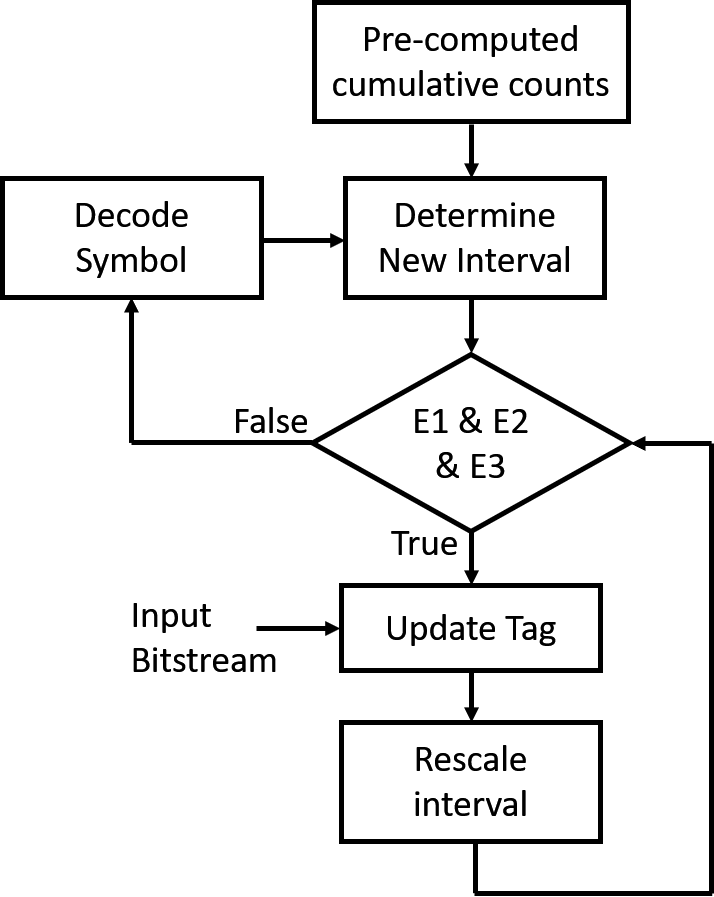
\includegraphics[width=0.5\textwidth]{./sdf/eit_46084_arithmetic_encoder_decoder/figures/ArithDecoderBlockDiagram.png}
	\caption{Block diagram of the algorithm for arithmetic decoding.} \label{fig:arithDecBlockDiagr}
\end{figure}

If either (\ref{eq:E1}) or (\ref{eq:E2}) is met, a new bit is read from the coded bit stream and added to the tag value multiplied by two. In the implemented code this is done right shifting the tag bits by one (discarding the most significant bit) and adding the new bit to it. If (\ref{eq:E3}) is met, the tag is updated in the same way but the new most significant bit is negated. When none of the conditions is met, a new symbol is decoded using the tag value normalized and the process continues until all symbols are decoded.


\subsection{Encoding and Decoding Simulation Results}

To test the implemented encoding and decoding algorithms, the system presented in Fig.\ref{fig:SystemBlockDiagr} was created in simulation. The system contains a binary source, the arithmetic encoding and decoding blocks and a bit-error-ratio computation block to ensure that the information is not degraded.

\begin{figure}[h]
	\centering
	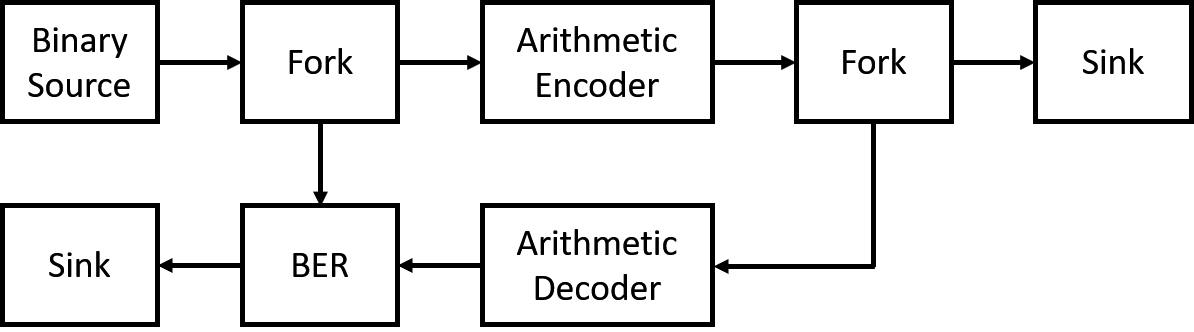
\includegraphics[width=0.85\textwidth]{./sdf/eit_46084_arithmetic_encoder_decoder/figures/TestSystemBlockDiagram.png}
	\caption{Block diagram of the floating point algorithm for arithmetic decoding.}\label{fig:SystemBlockDiagr}
\end{figure}

A test simulation with a total of 45360 bits and a probability of zero of 0.1 was performed. the number of bits of the encoder was changed from 2 to 5 and the code efficiency, given by (\ref{eq:codeEff}), was computed for each value. The results are presented in Fig.\ref{fig:CodeEff}. As expected, the code efficiency of the arithmetic algorithm is very close to optimum and increases as the number of coding bits increases.
\begin{equation} \label{eq:codeEff}
\eta = \frac{H(n)}{L}
\end{equation}

\begin{figure}[h]
	\centering
	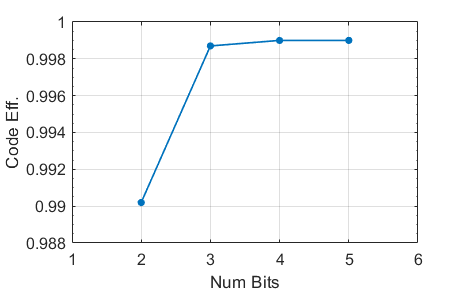
\includegraphics[width=0.65\textwidth]{./sdf/eit_46084_arithmetic_encoder_decoder/figures/CodeEff.png}
	\caption{Code efficiency variation with the number of coding bits.} \label{fig:CodeEff}
\end{figure}


\newpage

% bibliographic references for the section ----------------------------
\clearpage
%\printbibliography[heading=subbibliography]
\end{refsection}
\addcontentsline{toc}{subsection}{Bibliography}
\cleardoublepage
% --------------------------------------------------------------------- \fi
\ifdefined\miEstimator      \clearpage
\section{Mutual information estimation for a binary source}

\begin{refsection}

\begin{tcolorbox}	
\begin{tabular}{p{2.75cm} p{0.2cm} p{10.5cm}} 	
\textbf{Student Name}  &:& Mariana Ramos\\
\textbf{Starting Date} &:& July 24, 2018\\
\textbf{Goal}          &:& Test a mutual information estimator in a binary source.\\
\textbf{Directory}     &:& sdf/eit\_87071\_mutual\_information\_estimator.
\end{tabular}
\end{tcolorbox}

The main goal of this Mutual Information Estimator is to test the mutual information application in a binary source when it is connected to the receiver using a binary symmetric channel, which has a variable probability of error. The binary source should have equiprobable outputs, being $P(X=0) = P(X=1) = \frac{1}{2}$. However, this probability value can be set by the user. Moreover, the channel error probability can be set by the user and test the mutual information estimator for different error probabilities. The symbols are outputted by the binary source block with a certain probability. Then a add block follows the binary source, which will add errors in the sequence transmitted with a certain probability defined by the user. Mutual information estimator block receives the signal with errors as well as the sequence sent by the binary source. It will compare the two sequences, estimates channel error probability and $P(X=0)$ and finally calculates the entropy of the output symbols and the conditional entropy of the output symbols after observe the input symbols to calculate the mutual information between the two sequences. In sub section \ref{subsec:simulationmi} are presented numerical results and the theoretical results for further comparison. 

\subsection{Theoretical Analysis}
Mutual information is defined as a difference between the number of bits of information that the observer needs to determine the input channel symbol before observing the output bit symbol and the number of bits of information that he/she needs to determine the output bit symbol after observation. For a binary symmetric memoryless channel we can determine the mutual information using the formula:

\begin{equation}\label{eq:mutualinformation}
  I(X;Y) = H(Y) - H(Y|X),
\end{equation}
where $H(Y)$ is the entropy of the channel output symbols and $H(Y|X)$ is the conditional entropy of the channel output symbols depending on the channel input symbols. Regarding with a binary memoryless symmetric channel equation \ref{eq:mutualinformation} can be written as:

\begin{equation}\label{eq:mi_bsc}
  I(X;Y) = H(\bar{p}\alpha + p \bar{\alpha}) - H(p),
\end{equation}
as it is explained in section \ref{sec_mi}. In equation \ref{eq:mi_bsc} $p$ corresponds to the error probability of the binary symmetric memoryless channel and $\alpha$ corresponds to the probability of the input channel symbol.

In this case, the channel input symbols are equiprobable being $P(X=0) = P(X=1) = \alpha = \frac{1}{2}$. The error probability of the channel can be set by the user in the current setup. This way, if the error probability of the binary symmetric memoryless channel is lower that $\frac{1}{2}$, $\bar{p}\alpha + p \bar{\alpha} > p$ being the value calculated in equation \ref{eq:mi_bsc} positive. When $p=\frac{1}{2}$, the arguments of both entropy functions (conditional entropy and entropy of the output channel symbols) are equal, which means that its difference is zero and the average of amount of information transferred by the channel is also zero as shown in figure \ref{mifigure}.

\begin{figure}[H]
	\centering
	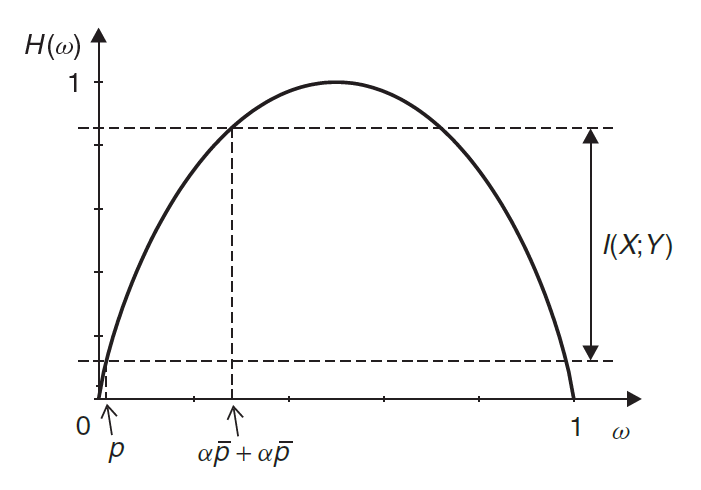
\includegraphics[width=0.6\textwidth]{./sdf/eit_87071_mutual_information_estimator/figures/mi_memoryless_binary_symmetric_channel.PNG}
	
	\caption{Graphical representation of average amount of information in the case of transmission using a binary symmetric memoryless channel. Figure from \cite{Wesolowski09}. }\label{mifigure}

\end{figure}

\subsection{Simulation Analysis}
\label{subsec:simulationmi}

\begin{figure}[H]
    \centering
        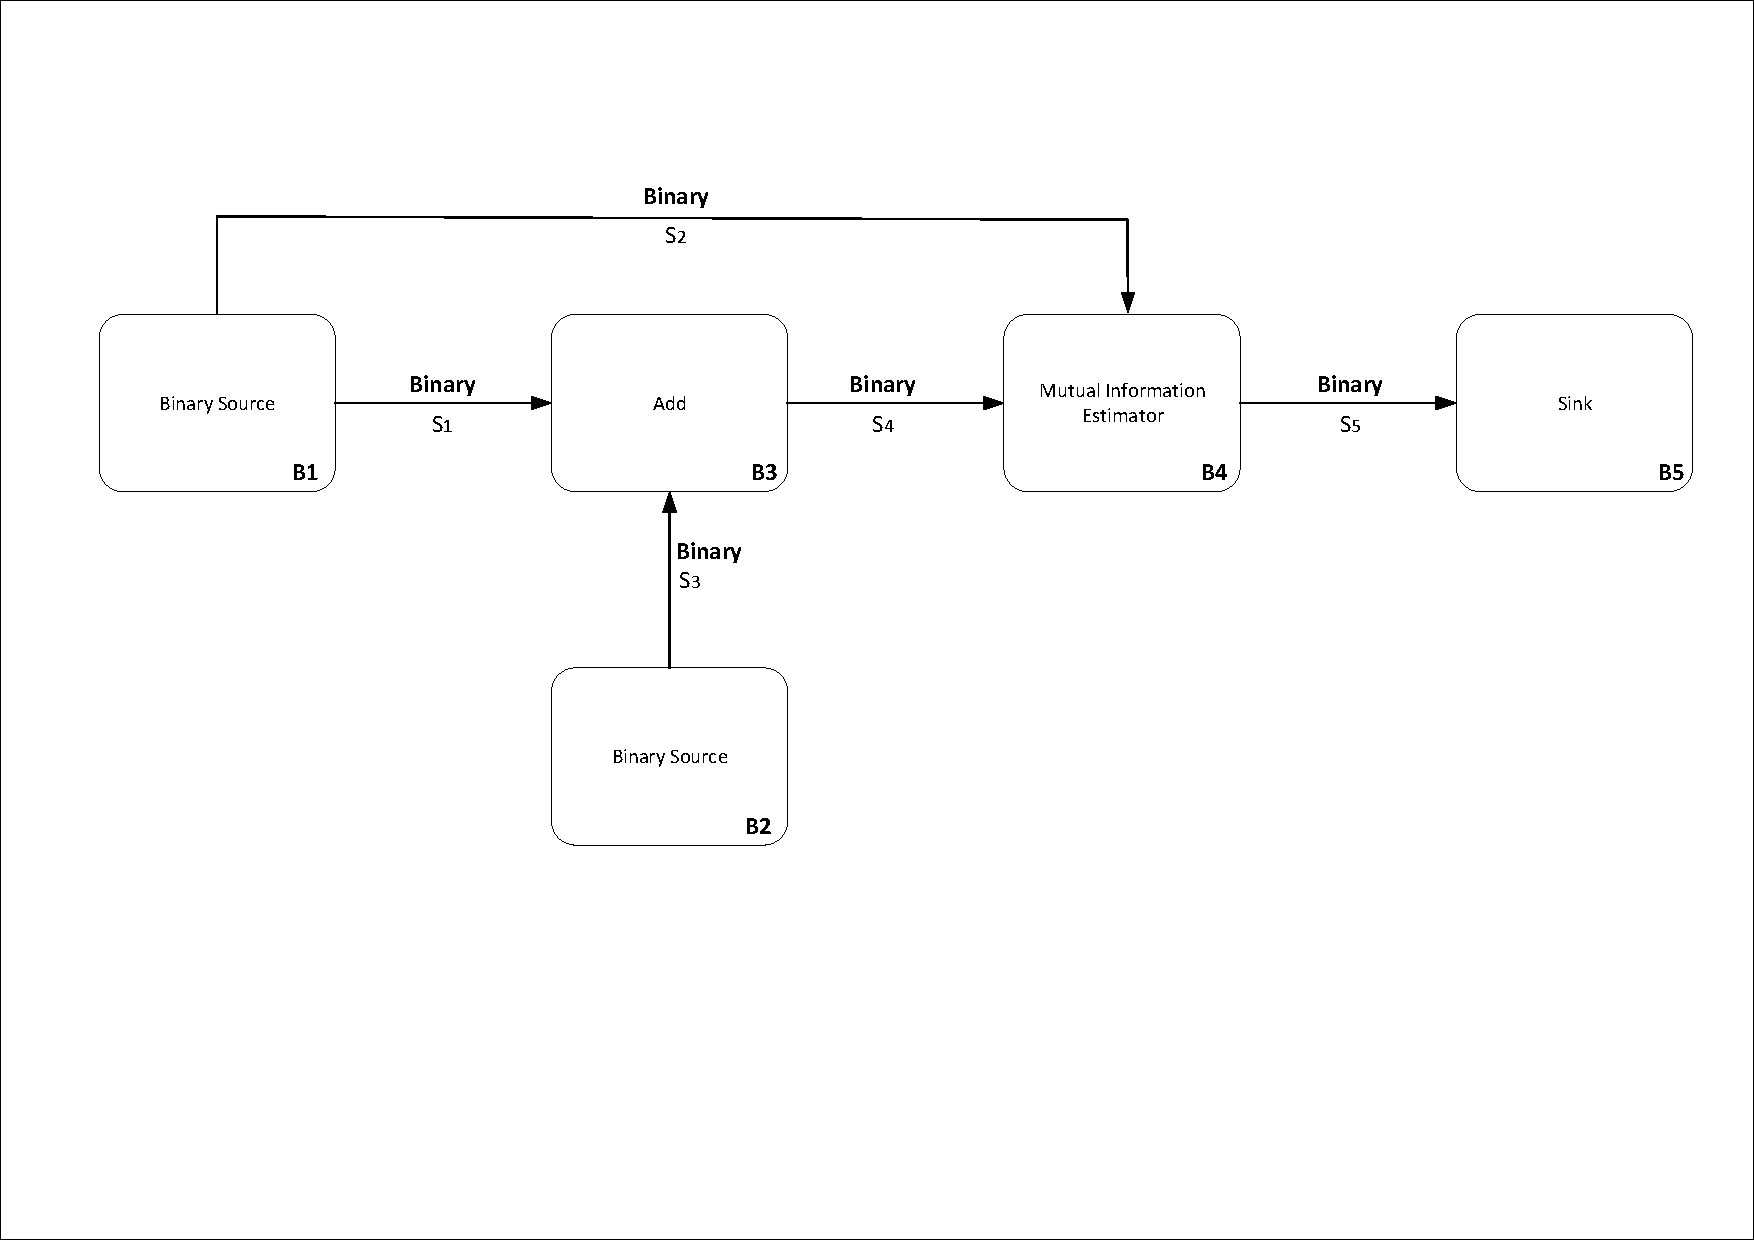
\includegraphics[clip, trim=1.0cm 6cm 1.0cm 2cm, width=0.90\textwidth]{./sdf/eit_87071_mutual_information_estimator/figures/block_diagram.pdf}
    \caption{Block diagram of the simulation implemented.}\label{fig:block_diagram}
\end{figure}

In figure \ref{fig:block_diagram} is shown the block diagram of the system implemented to test the block of mutual information estimator. In this case, the transmitter is the binary source \textbf{B1} which outputs bit 0 and bit 1 with the same probability, 0.5, randomly. The binary symmetric channel is represented by blocks \textbf{B2} and \textbf{B3}, being the first a binary source which outputs 0 with a probability $1-P_{\textrm{error}}$, where $P_{\textrm{error}}$ is defined by the user; and the second a adder block which introduces an error on the input bit sequence when the output of block \textbf{B2} is 1. Finally, \textbf{B4} is the block which estimates the mutual information between the input channel symbols and the output channel symbols and outputs a binary signal which takes value 1 when the input and output symbols are different and 0 otherwise. The functional description of this block is explained in detail in section \ref{sec_mi}.

In table \ref{tb:inputparameters2} are presented the input parameters of the system.

\begin{table}[H]
\centering
\caption{System Input Parameters}
\label{tb:inputparameters2}
\begin{tabular}{|c|c|c|}
\hline
\textbf{Parameter}                      & \textbf{Default Value}                                        \\ \hline
Perror                                  & 0.1                                                           \\ \hline
m                                       & 0                                                             \\ \hline
numberOfBits                            & 10                                                            \\ \hline

\end{tabular}
\end{table}

In table \ref{tb:signals2} are presented the system signals to implement the simulation presented in figure \ref{sim_qrng}.
\begin{table}[H]
\centering
\caption{System Signals}
\label{tb:signals2}
\begin{tabular}{|c|c|c|}
\hline
\textbf{Signal name}                            & \textbf{Signal type}                      \\ \hline
S1                                              &  Binary                                   \\ \hline
S2                                              &  Binary                                   \\ \hline
S3                                              &  Binary                                   \\ \hline
S4                                              &  Binary                                   \\ \hline
S5                                              &  Binary                                   \\ \hline
\end{tabular}
\end{table}

Table \ref{tb:signalsh} presents the header files used to implement the simulation as well as the specific parameters that should be set in each block. Finally, table \ref{tb:signalss} presents the source files.

\begin{table}[H]
\centering
\caption{Header Files}
\label{tb:signalsh}
\begin{tabular}{|c|c|c|}
\hline
\textbf{File name}                              & \textbf{Description}                                                          & \textbf{Status} \\ \hline
netxpto\_20180418.h                             &                                                                               &    \checkmark   \\ \hline
add\_20180620.h                                 &                                                                               &    \checkmark   \\ \hline
binary\_source\_20180723.h                      &                                                                               &    \checkmark   \\ \hline
mutual\_information\_estimator\_20180723.h      &                                                                               &    \checkmark   \\ \hline
sink.h                                          &                                                                               &    \checkmark   \\ \hline
\end{tabular}
\end{table}

\begin{table}[H]
\centering
\caption{Source Files}
\label{tb:signalss}
\begin{tabular}{|c|c|c|}
\hline
\textbf{File name}                                      & \textbf{Description} & \textbf{Status} \\ \hline
netxpto\_20180418.cpp                                   &                                                                               &    \checkmark   \\ \hline
add\_20180620.cpp                                       &                                                                               &    \checkmark   \\ \hline
binary\_source\_20180723.cpp                            &                                                                               &    \checkmark   \\ \hline
mutual\_information\_estimator\_20180723.cpp            &                                                                               &    \checkmark   \\ \hline
sink.cpp                                                &                                                                               &    \checkmark   \\ \hline
eit\_87071\_mutual\_information\_estimator\_sdf.cpp     &                                                                               &    \checkmark   \\ \hline
\end{tabular}
\end{table}

The system described above was implemented and it were acquired $1 \times 10^{5}$ symbols. Mutual information was calculated as well as the respective confidence intervals. The results are shown in table \ref{tb:data}.

\begin{table}[H]
\begin{tabular}{|c|c|c|c|c|c|c|}
\hline
$I(Y;X)$    & LB            & UB            & $H(Y|X)$      & $H(Y)$        & $p$           & $\bar{p}\alpha + p \bar{\alpha}$ \\ \hline
0.92226600  & 0.92392500    & 0.92060600    & 0.07772800    & 0.99999400    & 0.00954000    & 0.50147100                       \\ \hline
0.53179300  & 0.53488500    & 0.52870000    & 0.46820300    & 0.99999500    & 0.09975000    & 0.49871100                       \\ \hline
0.27601000  & 0.27878100    & 0.27324000    & 0.72398300    & 0.99999400    & 0.20103000    & 0.50147700                       \\ \hline
0.11982400  & 0.12183600    & 0.11781100    & 0.88017600    & 0.99999900    & 0.29909000    & 0.50052600                       \\ \hline
0.02746750  & 0.02848050    & 0.02645450    & 0.97253100    & 0.99999800    & 0.40274000    & 0.50074900                       \\ \hline
2.34E-08    & 9.71E-07      & -9.24E-07	    & 1.00000000    & 1.00000000    & 0.49991000    & 0.50000000	                   \\ \hline
0.0285718   & 0.0296043     & 0.0275392     & 0.9714280     & 1.0000000     & 0.5991800     & 0.4999960                        \\ \hline
0.1187460   & 0.1207510     & 0.1167410     & 0.8812540     & 1.0000000     & 0.7000300     & 0.5001840                        \\ \hline
0.2729990   & 0.2757600     & 0.2702380     & 0.7269990     & 0.9999980     & 0.7974500     & 0.5008510                        \\ \hline
0.5310040   & 0.5340970     & 0.5279110     & 0.4689960     & 1.0000000     & 0.9000000     & 0.4996960                        \\ \hline
0.9182140   & 0.9199120     & 0.9165160     & 0.0817859     & 1.0000000     & 0.9898500     & 0.5001960                        \\ \hline
\end{tabular}
\caption{Results acquired for $1 \times 10^{5}$ symbols acquisition.}
\label{tb:data}
\end{table}

After that the second line data from table \ref{tb:data} was chosen to represent graphically as shown in figure \ref{fig:datafig}.

\begin{figure}[h]
    \centering
        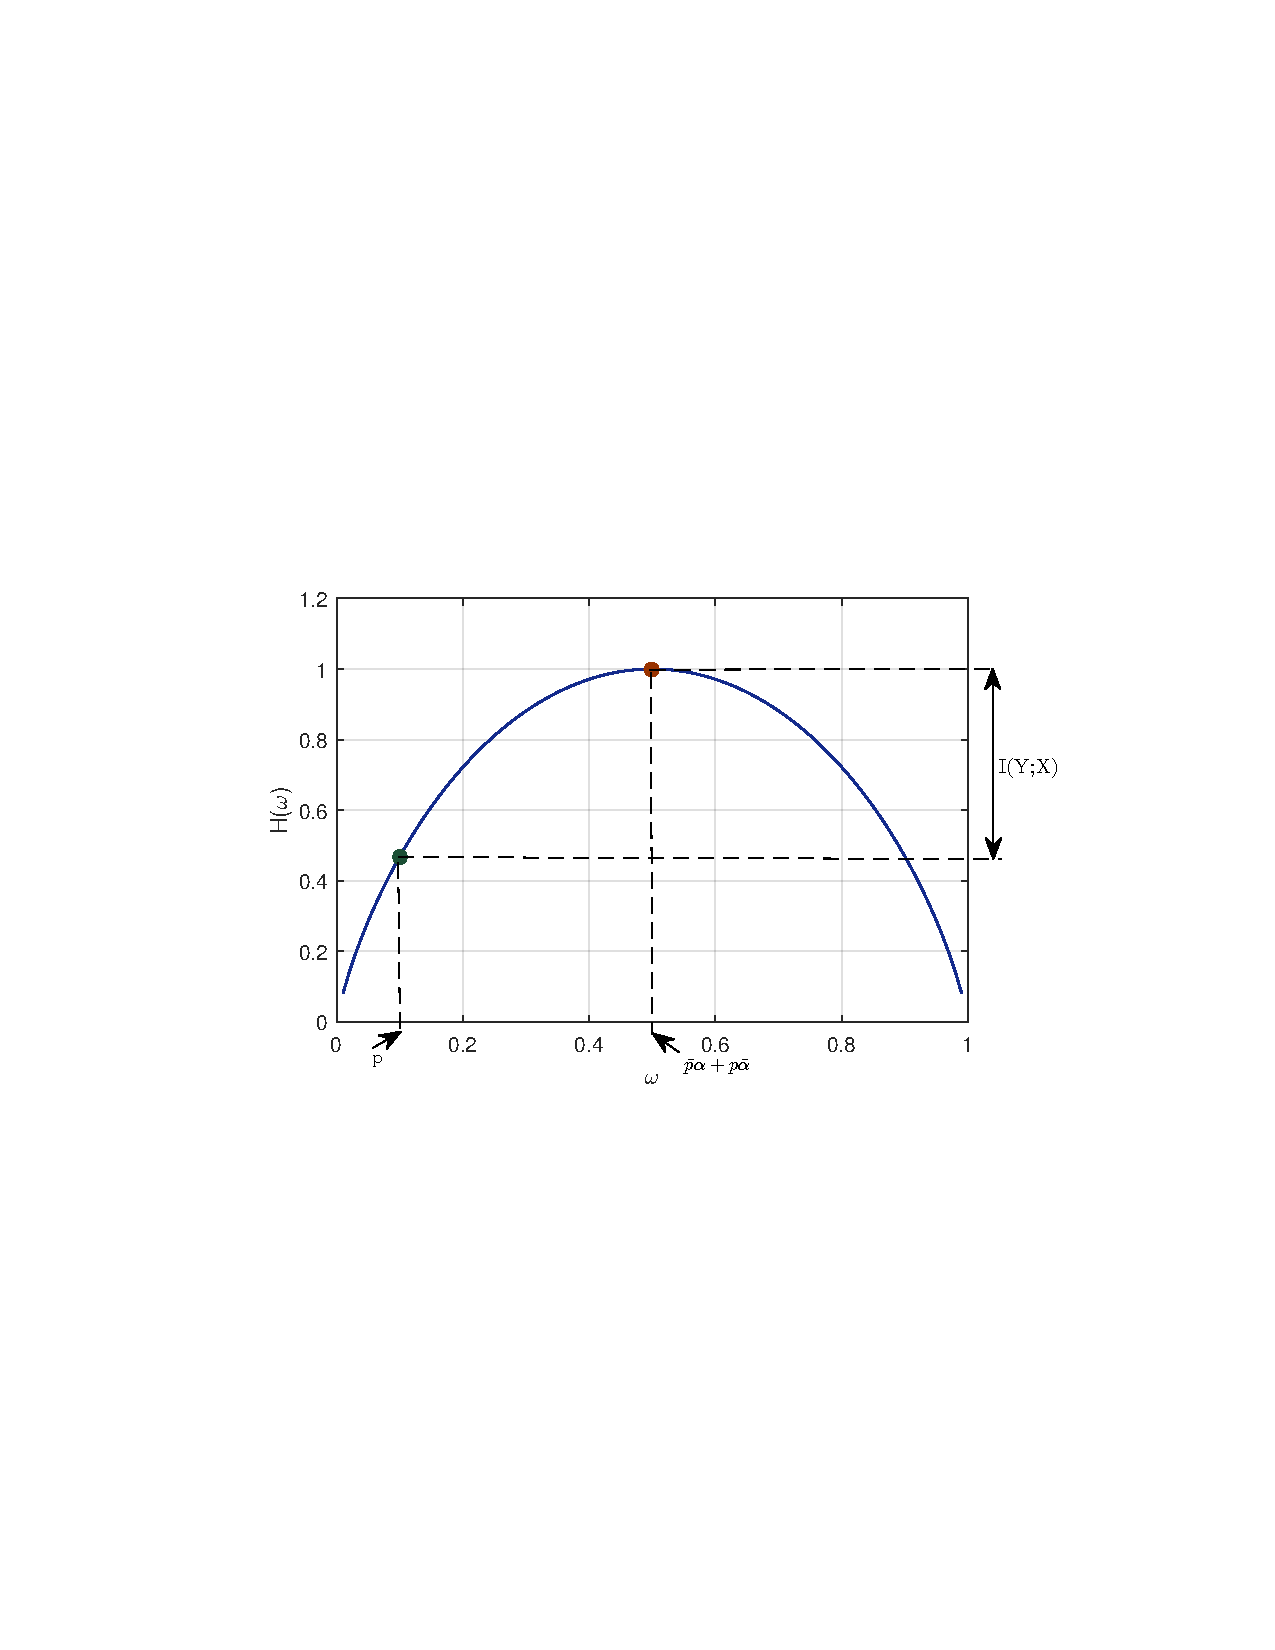
\includegraphics[clip, trim=1.0cm 9cm 1.0cm 9cm, width=0.90\textwidth]{./sdf/eit_87071_mutual_information_estimator/figures/fig1.pdf}
    \caption{Numerical results representation for mutual information calculation. $I(Y;X) = H(Y) - H(Y|X) = 0.5318$; $H(Y|X) = 0.4680$; $H(Y) = 1.0000$; $p=0.0998$; $\bar{p}\alpha + p \bar{\alpha} = 0.4987$.}\label{fig:datafig}
\end{figure}

Results shown in figure \ref{fig:datafig} meet the theoretical representation shown in figure \ref{mifigure}. Moreover, mutual information was calculated for a binary symmetric channel using different channel error probabilities ($p$), theoretically, using equation \ref{eq:mi_bsc}. Both, theoretical and numerical values with the respective confidence intervals of mutual information were plotted in figure \ref{fig:theornum}. As one can see in the figure, the numerical results meet the theoretical values of mutual information, which means that the mutual information estimator has the expected performance.

\begin{figure}[h]
    \centering
        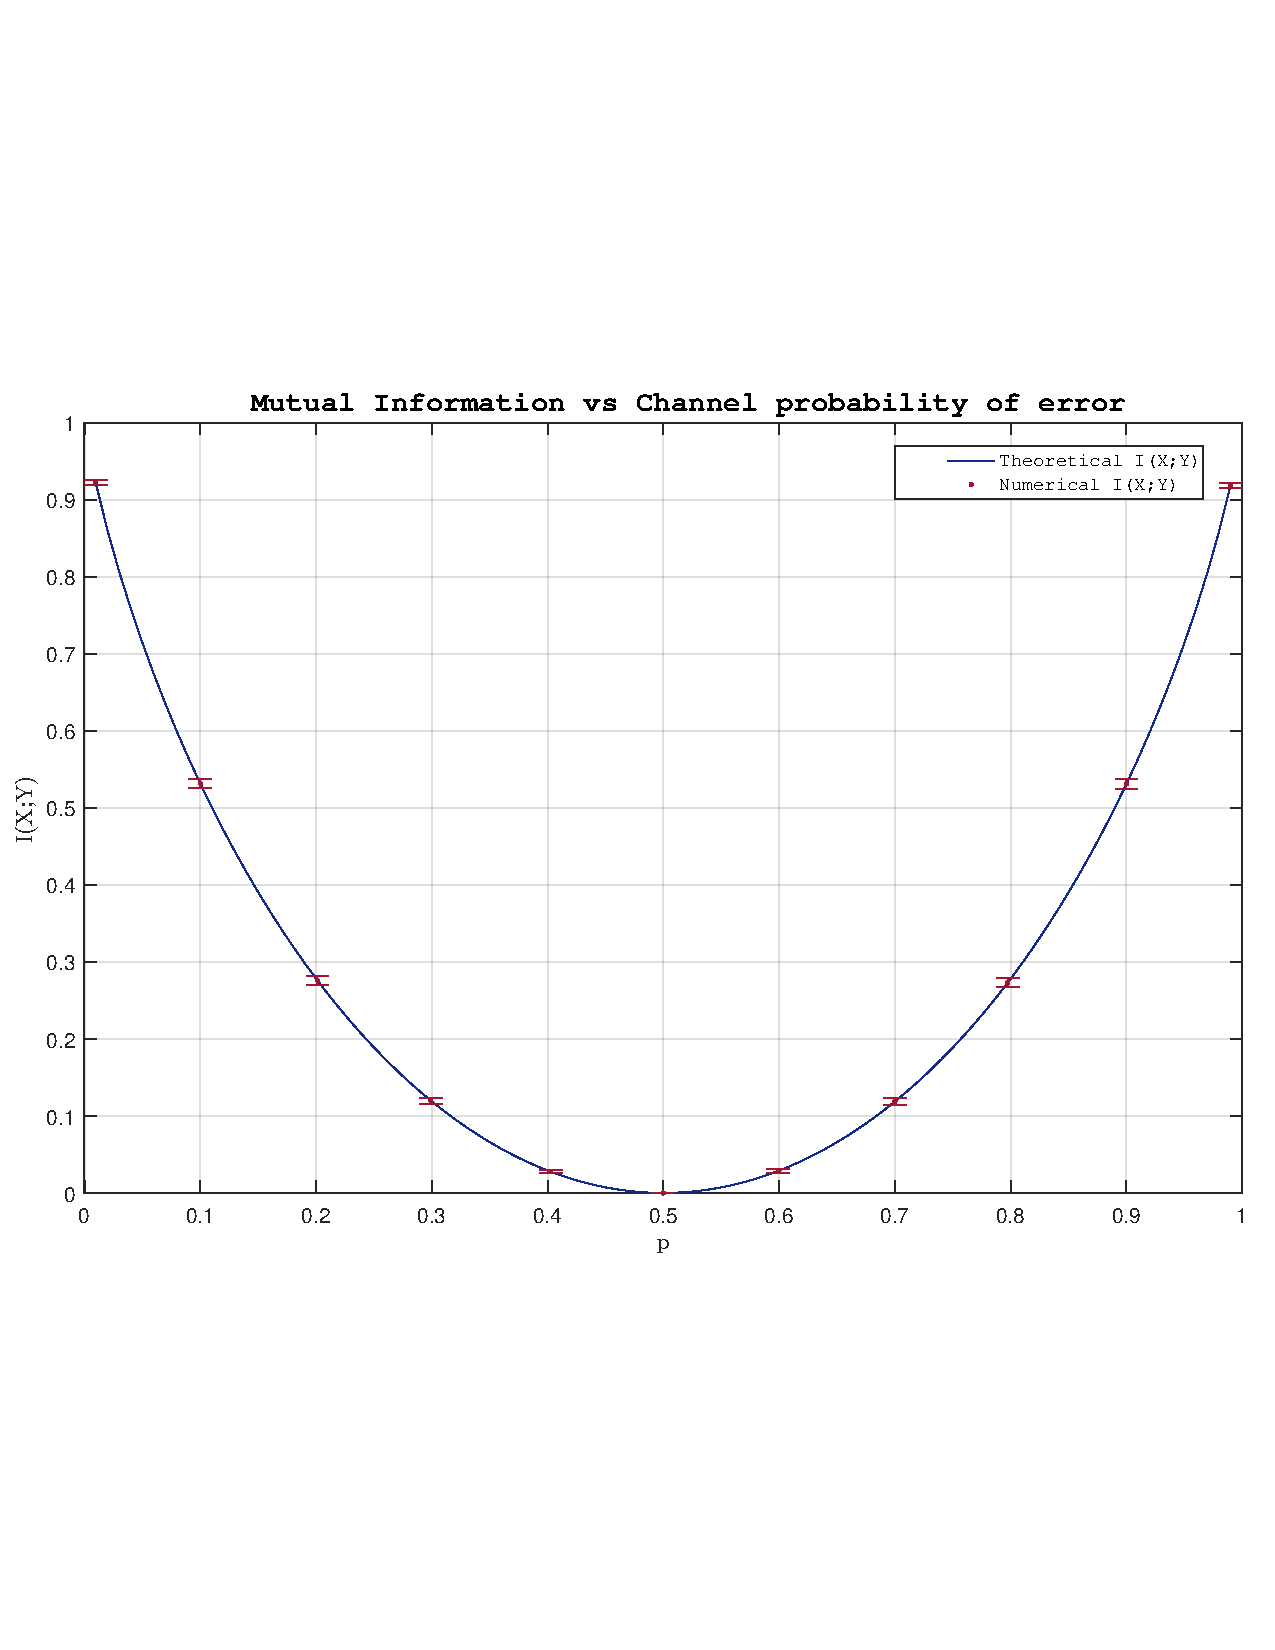
\includegraphics[clip, trim=0.05cm 6cm 0.5cm 6cm, width=0.90\textwidth]{./sdf/eit_87071_mutual_information_estimator/figures/fig2.pdf}
    \caption{Numerical values of mutual information for different channel probability errors Vs theoretical mutual information.}\label{fig:theornum}
\end{figure}




% bibliographic references for the section ----------------------------
\clearpage
\printbibliography[heading=subbibliography]
\end{refsection}
\addcontentsline{toc}{subsection}{Bibliography}
\cleardoublepage
% --------------------------------------------------------------------- \fi
\ifdefined\dynamicHED       %\usepackage{setspace}

\clearpage
\section{Dynamic Huffman Coder and Decoder}

\begin{refsection}

\begin{tcolorbox}	
\begin{tabular}{p{2.75cm} p{0.2cm} p{10.5cm}} 	
\textbf{Students Name}  &:& Cristiano Ferreira Gon\c{c}alves (10/06/2018 - 29/06/2018) \\
\textbf{Starting Date} &:& June 10, 2018\\
\textbf{Goal}          &:& Huffman coding and decoding of text.
\end{tabular}
\end{tcolorbox}

Dynamic Huffman code can compress text very effectively for medium-long texts without previous knowledge of the characters probability.

\subsection{Code Analysis}

\hspace{5mm} This code is stored and based on a Huffman tree, for example as the one of Figure \ref{fig:hufftree}. This tree stores in its leafs $($bottom nodes$)$ the characters. The code is attributed by the path from the root to each character, for each level of the tree is attributed an '1' if the path follows through the right soon or a '0' if it follows left.

\begin{figure}[H]
	\centering
	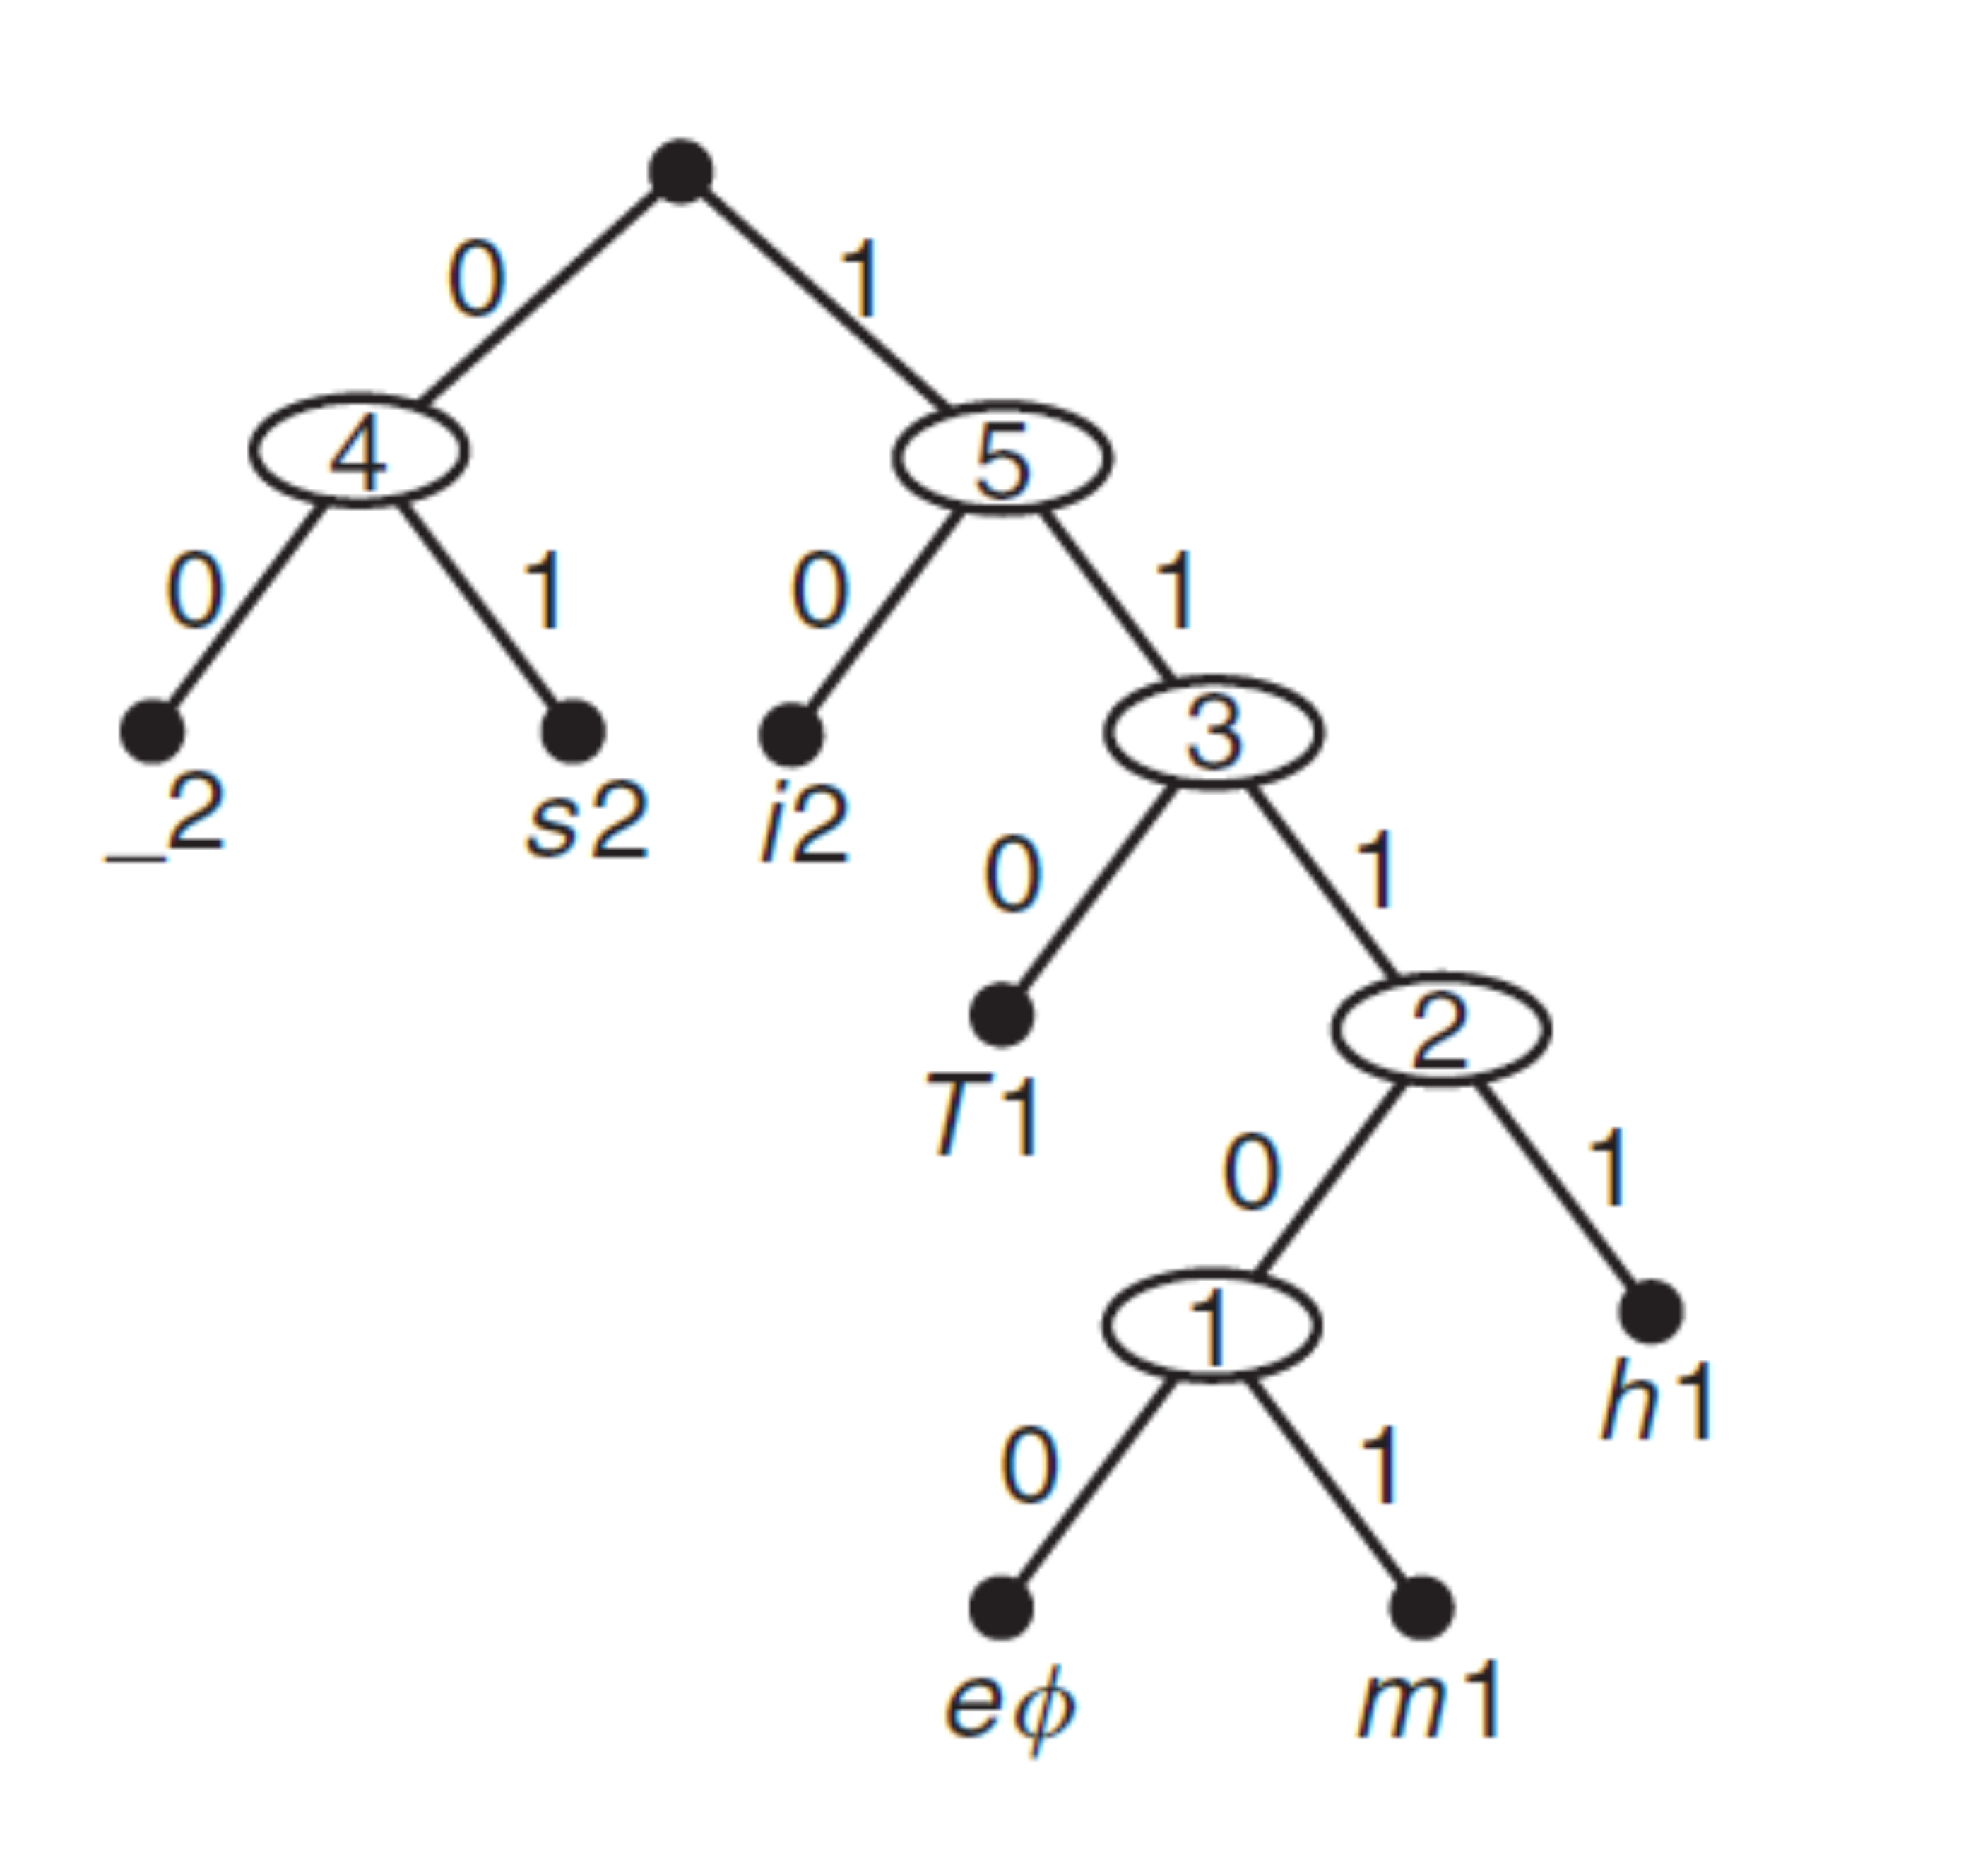
\includegraphics[width=0.5\textwidth,height=7cm]{./sdf/eit_64926_dynamic_huffman_encoder_decoder/figures/HuffTree.png}
	\caption{Ordered Huffman tree example (figure from \cite{DigComm}).}\label{fig:hufftree}
\end{figure}

For each of the nodes 4 variables are stored:
\begin{itemize}
	\item The character stored in the node;
	\item The frequency of the character $($number of times it appeared$)$;
	\item The pointer to the right soon node;
	\item The pointer to the left soon node.
\end{itemize}
\vspace{2cm}

When a new character is received two cases can happen:
\begin{itemize}
\item The character already exists and its frequency is incremented by one.
\item The character do not exists on the tree and a new node is added for it.
\end{itemize}

For the last case, the node is added as right soon of the previous empty node and the new empty node becomes the left soon of the previous empty node.\\
After each modification the tree is reordered so its leafs from left to right and bottom-up are in ascending order of frequency. For the case described in Figure \ref{fig:hufftree}, it would be:
\[ e\emptyset \quad m1 \quad 1 \quad h1 \quad T1 \quad 2 \quad \_2 \quad s2 \quad i2 \quad 3 \quad 4 \quad 5 \]
\hspace{5mm} The previous sequence is correctly ordered in terms of frequency. However for the example of Figure \ref{fig:hufftree2} the order would be:
\[ e\emptyset \quad \_2 \quad 2 \quad T1 \quad h1 \quad s2 \quad i2 \quad 3 \quad 3 \quad 5 \]

\begin{figure}[H]
	\centering
	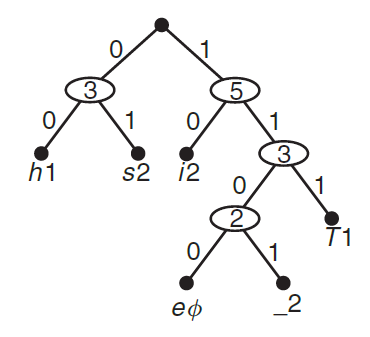
\includegraphics[width=0.5\textwidth,height=7cm]{./sdf/eit_64926_dynamic_huffman_encoder_decoder/figures/HuffTree2.png}
	\caption{Not ordered Huffman tree example (figure from \cite{DigComm}).}\label{fig:hufftree2}
\end{figure}


For this case the nodes \_2 and h1 should be swapped. This swap should be done between the first higher node $($\_2 instead of 2$)$ and the last lower one $($h1 instead of T1$)$ so the sub-tree becomes always ordered and the tree gets fully ordered faster.

\subsection{Practical Test}

\hspace{5mm} The algorithm has been implemented and the respective program used to encode the following text:\\
{\tiny "Nowadays, the power amplifier (PA) design paradigm is changing. Modern wireless networks push for PAs bandwidth, higher efficiencies and improved linearity requiring the use of more complex architectures [1][2]. Therefore, although the PA design methodology based on load-pull and S-parameter measurements obtained good results in the past [3], it is now very difficult to achieve the required figures of merit maintaining these design methodologies. This being the case, the use of CAD programs with accurate nonlinear models becomes of paramount importance. Such models have been intensively described in literature [4][5], and are particularly interesting in the case of high frequency designs, mainly for the future mm-wave 5G networks, since at these frequencies the load-pull measurements are much harder to perform and the required equipment is very specific and expensive. The problem with this approach is that the obtained PA performance is strongly dependent on the accuracy of the used device models, which is strongly correlated with the quality of the measurements performed during the nonlinear model extraction [6].
Gallium Nitride (GaN) High Electron Mobility Transistors (HEMTs) are predominantly adopted on these new mm-wave state-of-art PAs due to their advantages in terms of power density, cut-off frequency and high thermal conductivity. However, these devices are still affected by many frequency dispersive phenomena as thermal and trapping effects [7]-[9]. These problems cause a substantial discrepancy between their static and dynamic characteristics. Thus, in order to properly model their behavior isodynamic measurements are necessary, which leads to more sophisticated measurement setups.
There are two main approaches to characterize these new devices: (i) Continuous wave (CW) excitations to cover the entire I/V plane [10], which implies a complicated curve-fitting process to simultaneously extract the resistive and reactive components of the device. (ii) Pulsed I/V and S-parameter measurements [11][12], for which a system that allows the generation of very fast, high-power and arbitrary waveform pulses is necessary. In these last ones, the capability to generate arbitrary bias signals is of remarkable importance, because it allows to generate specific waveforms that are necessary to guarantee isothermal measurements and avoid dispersive phenomena [11]. There are already pulsed measurements systems able to generate 100 V and 7 A pulses with 600 ns settling time [13]-[15], and some modern pulsers that can handle 5000 W or even higher instantaneous power [16][17]. However, they are very expensive and unable to generate the necessary waveforms.
Compared to the available ones, this paper presents a cost effective and more versatile measurement system, which allows the use of arbitrary waveform signals. This makes possible to obtain accurate and isodynamic pulsed measurements. Thus, the main contributions of this paper are the power head and respective characterization signal waveform design. To test the implemented system a 15 W GaN device from Wolfspeed was measured and shown to be mainly affected by drain lag and temperature effects. The second part of this paper is dedicated to the measurement setup and pulser implementation. The third section will be devoted to the waveform design. Lastly, in the fourth section, the measurements will be compared with I/V curves obtained from the integration of the small signal transcondutance $($g\textsubscript{m} $)$ and output conductance $($g\textsubscript{ds}$)$. The good agreement obtained between all the sets of curves attests its isodynamic behavior."}\\

This text has been encoded without any error in 60\% of its original size, as shown in Figure \ref{fig:encodedtext}. The total size decreased from 3.6KB to 2.2KB.

\begin{figure}[H]
	\centering
	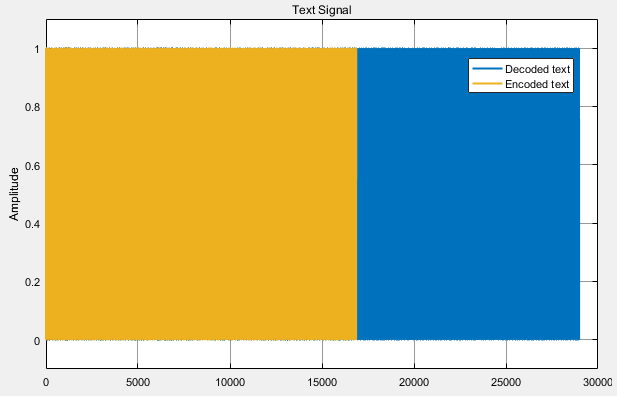
\includegraphics[width=0.7\textwidth,height=7cm]{./sdf/eit_64926_dynamic_huffman_encoder_decoder/figures/textSignals.png}
	\caption{Matlab visualization of the encoded and decoded signals of the example text.}\label{fig:encodedtext}
\end{figure}

% Bibliography
\newpage
\clearpage
\printbibliography[heading=subbibliography]
\end{refsection}
\addcontentsline{toc}{subsection}{Bibliography}
\cleardoublepage \fi
\ifdefined\mQAM         	\input{./sdf/m_qam_system/m_qam_system} \fi
\ifdefined\lBmQAM       	\input{./sdf/low_baud_m_qam_system/low_baud_m_qam_system} \fi
\ifdefined\rofKK        	\input{./sdf/kramers_kronig_transceiver/kramers_kronig_transceiver} \fi
\ifdefined\dsp          	\input{./sdf/dsp_laser_phase_compensation/dsp_laser_phase_compensation} \fi
\ifdefined\quantumRNG   	\input{./sdf/quantum_random_number_generator/quantum_random_number_generator} \fi
\ifdefined\bb           	\input{./sdf/bb84_with_discrete_variables/bb84_with_discrete_variables} \fi
\ifdefined\qokd         	\input{./sdf/qokd_with_discrete_variables/qokd_with_discrete_variables} \fi
\ifdefined\dv               \input{./sdf/dv_polarization_encoding_system/dv_polarization_encoding_system} \fi
\ifdefined\bob              \input{./sdf/dv_polarization_encoding_system_bob_processor/dv_polarization_encoding_system_bob_processor}\fi
\ifdefined\quantumA     	\input{./sdf/quantum_noise/quantum_noise} \fi
\ifdefined\cvQuantum        \input{./sdf/cv_system/cv_system} \fi
\ifdefined\qkdCvWithoutBS   \input{./sdf/qkd_with_cv_without_base_switching/qkd_with_cv_without_base_switching} \fi
\ifdefined\intradyne        \input{./sdf/intradyne_cv_system/intradyne_cv_system} \fi
\ifdefined\classicalMpc     \input{./sdf/classical_mpc/classical_mpc} \fi
\ifdefined\quantumMpc       \input{./sdf/quantum_mpc/quantum_mpc} \fi
\ifdefined\secureMPC        \input{./sdf/secure_multiparty_computation/secure_multiparty_computation} \fi
\ifdefined\secureMPC        \input{./sdf/tiny_garble/tiny_garble} \fi

%
% ------------------------------------------------------------------------
\chapter{Library}

\clearpage

\section{ADC}

\begin{tcolorbox}	
	\begin{tabular}{p{2.75cm} p{0.2cm} p{10.5cm}} 	
		\textbf{Header File}   &:& adc$\_*$.h \\
		\textbf{Source File}   &:& adc$\_*$.cpp \\
        \textbf{Version}       &:& 20180423 (Celestino Martins) \\
	\end{tabular}
\end{tcolorbox}

This super block block simulates an analog-to-digital converter (ADC), including signal resample and quantization. It receives two real input signal and outputs two real signal with the sampling rate defined by ADC sampling rate, which is externally configured using the resample function, and quantized signal into a given discrete values.

\subsection*{Input Parameters}

\begin{table}[h]
	\centering
	\begin{tabular}{|c|c|c|c|c|c|cccc}
		\cline{1-4}
		\textbf{Parameter} & \textbf{Unity} & \textbf{Type} & \textbf{Values} &   \textbf{Default}& \\ \cline{1-5}
        samplingPeriod & -- & double & any & $--$ \\ \cline{1-5}
        rFactor       & --    & double & any & $1$ \\ \cline{1-5}	
		resolution & bits  & double & any & $inf$ \\ \cline{1-5}	
        maxValue   & volts & double & any & $1.5$ \\ \cline{1-5}	
        minValue   & volts & double & any    & $-1.5$ \\ \cline{1-5}	
	\end{tabular}
	\caption{ADC input parameters}
	\label{table:ADC_in_par}
\end{table}

\subsection*{Methods}

ADC(vector$<$Signal *$>$ \&InputSig, vector$<$Signal *$>$ \&OutputSig);
\bigbreak
//void setResampleSamplingPeriod(double sPeriod) { B1.setSamplingPeriod(sPeriod); B2.setSamplingPeriod(sPeriod); };
\bigbreak
void setResampleOutRateFactor(double OUTsRate) { B01.setOutRateFactor(OUTsRate); B02.setOutRateFactor(OUTsRate); }
\bigbreak
void setQuantizerSamplingPeriod(double sPeriod) { B03.setSamplingPeriod(sPeriod); B04.setSamplingPeriod(sPeriod); }
\bigbreak
void setSamplingPeriod(double sPeriod) { B03.setSamplingPeriod(sPeriod); };
\bigbreak
void setQuantizerResolution(double nbits) { B03.setResolution(nbits); B04.setResolution(nbits); }
\bigbreak
void setQuantizerMaxValue(double maxvalue) { B03.setMaxValue(maxvalue); B04.setMaxValue(maxvalue);}
\bigbreak
void setQuantizerMinValue(double minvalue) { B03.setMinValue(minvalue); B04.setMinValue(minvalue); }

\subsection*{Functional description}

This super block is composed of two blocks, resample and quantizer. It can perform the signal resample according to the defined input parameter \textit{rFactor} and signal quantization according to the defined input parameter \textit{nBits}.


\pagebreak
\subsection*{Input Signals}

\subparagraph*{Number:} 2

\subsection*{Output Signals}

\subparagraph*{Number:} 2

\subparagraph*{Type:} Electrical complex signal

\subsection*{Examples}

\subsection*{Sugestions for future improvement}



\clearpage

\section{Add}

\begin{tcolorbox}	
\begin{tabular}{p{2.75cm} p{0.2cm} p{10.5cm}} 	
\textbf{Header File}   &:& add.h \\
\textbf{Source File}   &:& add.cpp \\
\textbf{Version}       &:& 20180118
\end{tabular}
\end{tcolorbox}

\subsection*{Input Parameters}

This block takes no parameters.

\subsection*{Functional Description}

This block accepts two signals and outputs one signal built from a sum of the two inputs. The input and output signals must be of the same type, if this is not the case the block returns an error.

\subsection*{Input Signals}

\textbf{Number}: 2\\
\textbf{Type}: Real, Complex or Complex\_XY signal (ContinuousTimeContinuousAmplitude)

\subsection*{Output Signals}

\textbf{Number}: 1\\
\textbf{Type}: Real, Complex or Complex\_XY signal (ContinuousTimeContinuousAmplitude)

%\end{document}

\clearpage

\section{Arithmetic Encoder}

\begin{tcolorbox}	
	\begin{tabular}{p{2.75cm} p{0.2cm} p{10.5cm}} 	
		\textbf{Header File}   &:& arithmetic\_encoder.h \\
		\textbf{Source File}   &:& arithmetic\_encoder.cpp \\
        \textbf{Version}       &:& 20180719 (Diogo Barros) \\
	\end{tabular}
\end{tcolorbox}

This block implements the integer version of the arithmetic encoding algorithm, given the symbol counts, the number of bits per symbol and the number of symbols to encode.
The block takes a binary input stream and outputs the encoded binary stream.

\subsection*{Input Parameters}

\begin{table}[h]
	\centering
	\begin{tabular}{|c|c|c|c|cccc}
		\cline{1-4}
		\textbf{Parameter} & \textbf{Type} & \textbf{Values} & \textbf{Default} & \\ \cline{1-5}
        SeqLen 	   & unsigned int 		  & any & $--$ 	\\ \cline{1-5}
		BitsPerSymb& unsigned int         & any & $--$ 	\\ \cline{1-5}	
	    SymbCounts & vector<unsigned int> & any & $--$  \\ \cline{1-5}	
	\end{tabular}
	\caption{Arithmetic encoder block input parameters.}
	\label{table:arith_enc_in_par}
\end{table}

\subsection*{Methods}

	bool runBlock(void)
\bigbreak
void initialize(void);
\bigbreak
void init(const unsigned int\& SeqLen, const unsigned int\& BitsPerSymb,
const vector<unsigned int>\& SymbCounts);
\bigbreak


\subsection*{Functional description}

This block implements the integer version of the arithmetic encoding algorithm, given the symbol counts, the number of bits per symbol and the number of symbols to encode.


\pagebreak
\subsection*{Input Signals}

\subparagraph*{Number:} 1

\subsection*{Output Signals}

\subparagraph*{Number:} 1

\subparagraph*{Type:} binary

\subsection*{Examples}

\subsection*{Sugestions for future improvement}



\clearpage

\section{Arithmetic Decoder}

\begin{tcolorbox}	
	\begin{tabular}{p{2.75cm} p{0.2cm} p{10.5cm}} 	
		\textbf{Header File}   &:& arithmetic\_decoder.h \\
		\textbf{Source File}   &:& arithmetic\_decoder.cpp \\
        \textbf{Version}       &:& 20180719 (Diogo Barros) \\
	\end{tabular}
\end{tcolorbox}

This block implements the integer version of the arithmetic decoding algorithm, given the symbol counts, the number of bits per symbol and the number of symbols to encode.
The block takes an encoded binary input stream and outputs the decoded binary stream.

\subsection*{Input Parameters}

\begin{table}[h]
	\centering
	\begin{tabular}{|c|c|c|c|cccc}
	\cline{1-4}
	\textbf{Parameter} & \textbf{Type} & \textbf{Values} & \textbf{Default} & \\ \cline{1-5}
	SeqLen 	   & unsigned int 		  & any & $--$ 	\\ \cline{1-5}
	BitsPerSymb& unsigned int         & any & $--$ 	\\ \cline{1-5}	
	SymbCounts & vector<unsigned int> & any & $--$  \\ \cline{1-5}	
	\end{tabular}
	\caption{Arithmetic decoding block input parameters.}
	\label{table:arith_dec_in_par}
\end{table}

\subsection*{Methods}

bool runBlock(void)
\bigbreak
void initialize(void);
\bigbreak
void init(const unsigned int\& SeqLen, const unsigned int\& BitsPerSymb,
const vector<unsigned int>\& SymbCounts);
\bigbreak

\subsection*{Functional description}

This block implements the integer version of the arithmetic decoding algorithm, given the symbol counts, the number of bits per symbol and the number of symbols to encode.
The block takes an encoded binary input stream and outputs the decoded binary stream.


\pagebreak
\subsection*{Input Signals}

\subparagraph*{Number:} 2

\subsection*{Output Signals}

\subparagraph*{Number:} 2

\subparagraph*{Type:} Electrical complex signal

\subsection*{Examples}

\subsection*{Sugestions for future improvement}



\clearpage

\section{Alice QKD}

\maketitle
This block is the processor for Alice does all tasks that she needs. This block accepts binary, messages, and real continuous time signals. It produces messages, binary and real discrete time signals.


\subsection*{Input Parameters}

	\begin{itemize}
		\item double RateOfPhotons\{1e3\}
	
		\item int StringPhotonsLength\{ 12 \}
	\end{itemize}

\subsection*{Methods}
    AliceQKD (vector <Signal*> \&inputSignals, vector <Signal*> \&outputSignals) : Block(inputSignals, outputSignals) \{\};

	void initialize(void);

	bool runBlock(void);

	void setRateOfPhotons(double RPhotons) \{ RateOfPhotons = RPhotons; \};
	double const getRateOfPhotons(void) \{ return RateOfPhotons; \};

	void setStringPhotonsLength(int pLength) \{ StringPhotonsLength = pLength; \};
	int const getStringPhotonsLength(void) \{ return StringPhotonsLength; \};


\subsection*{Functional description}

This block receives a sequence of binary numbers (1's or 0's) and a clock signal which will set the rate of the signals produced to generate single polarized photons. The real discrete time signal \textbf{SA\_1} is generated based on the clock signal and the real discrete time signal \textbf{SA\_2} is generated based on the random sequence of bits received through the signal \textbf{NUM\_A}. This last sequence is analysed by the polarizer in pairs of bits in which each pair has a bit for basis choice and other for direction choice.

This block also produces classical messages signals to send to Bob as well as binary messages to the mutual information block with information about the photons it sent.

\subsection*{Input Signals}
\paragraph*{Number}: 3
\paragraph*{Type}: Binary, Real Continuous Time and Messages signals.

\subsection*{Output Signals}
\paragraph*{Number}: 3
\paragraph*{Type}: Binary, Real Discrete Time and Messages signals.

\subsection*{Examples}


\subsection*{Sugestions for future improvement}




\clearpage

\section{Ascii Source}

\begin{tcolorbox}	
	\begin{tabular}{p{2.75cm} p{0.2cm} p{10.5cm}} 	
		\textbf{Header File}   &:& ascii\_source\_*.h \\
		\textbf{Source File}   &:& ascii\_source\_*.cpp \\
        \textbf{Version}       &:& 20180828 (Andr\'e Mourato)
	\end{tabular}
\end{tcolorbox}

\maketitle
This block generates an ascii signal and can work in different modes:

\begin{multicols}{3}
\begin{enumerate}
	\item Terminate
	\item Cyclic
	\item AppendZeros
\end{enumerate}
\end{multicols}

This blocks doesn't accept any input signal. It produces any number of output signals.

\subsection*{Input Parameters}

\begin{table}[h]
	\centering
	\begin{tabular}{|c|c|p{60mm}|c|ccp{60mm}}
		\cline{1-4}
		\textbf{Parameter} & \textbf{Type} & \textbf{Values} &   \textbf{Default}& \\ \cline{1-4}
		mode & AsciiSourceMode & Terminate, AppendZeros, Cyclic & Terminate \\ \cline{1-4}
        asciiString & string & any & ``" \\ \cline{1-4}
        asciiFilePath & string & any & ``text\_file.txt" \\ \cline{1-4}
        numberOfCharacters & int & $ \in [0,\infty[$ & 1000 \\ \cline{1-4}

	\end{tabular}
	\caption{Binary source input parameters}
	\label{table:bin_sour_in_par}
\end{table}

\subsection*{Methods}

AsciiSource(vector$\langle$Signal *$\rangle$ \&InputSig, vector$\langle$Signal *$\rangle$ \&OutputSig) :Block(InputSig, OutputSig)\{\};
\bigbreak	
void initialize(void);
\bigbreak	
bool runBlock(void);
\bigbreak
void setMode(AsciiSourceMode m);
\bigbreak
AsciiSourceMode const getMode(void);
\bigbreak
void setAsciiString(string s);
\bigbreak
string getAsciiFilePath();
\bigbreak
void setNumberOfCharacters(int n);
\bigbreak
int getNumberOfCharacters();
\bigbreak

\subsection*{Functional description}

The \textit{mode} parameter allows the user to select one of the operation modes of the ascii source.

\subparagraph*{Terminate}
The resulting ascii signal will be the $asciiString$ sequence of characters.

\subparagraph*{AppendZeros}
The resulting ascii signal will be a sequence of characters starting with $asciiString$ with zeros (null character) concatenated to the right until $numberOfCharacters$ characters have been generated.

\subparagraph*{Cyclic}
The resulting ascii signal will be a sequence of characters in which $asciiString$ is concatenated to the right of the string until $numberOfCharacters$ characters have been generated.

\subsection*{Input Signals}

\subparagraph*{Number:} 0

\subsection*{Output Signals}

\subparagraph*{Number:} 1 or more

\subparagraph*{Type:} Ascii


\clearpage

\section{Ascii To Binary}

\begin{tcolorbox}	
	\begin{tabular}{p{2.75cm} p{0.2cm} p{10.5cm}} 	
		\textbf{Header File}   &:& ascii\_to\_binary\_*.h \\
		\textbf{Source File}   &:& ascii\_to\_binary\_*.cpp \\
        \textbf{Version}       &:& 20180905 (Andr\'e Mourato)
	\end{tabular}
\end{tcolorbox}

\subsection*{Methods}

AsciiToBinary(vector$\langle$Signal *$\rangle$ \&InputSig, vector$\langle$Signal *$\rangle$ \&OutputSig) :Block(InputSig, OutputSig)\{\};
\bigbreak
void initialize(void);
\bigbreak
bool runBlock(void);
\bigbreak

\subsection*{Functional description}

Figure \ref{AsciiSignalImage} shows an example of an input signal that can be passed as argument. This signal contains three characters: a, b and c. Each character can be represented by 8 bits, according to the Ascii Table. The values to these three characters are respectively: $01100001$, $1100010$ and $1100011$.
The block AsciiToBinary will convert the characters a, b and c to their respective binary codes. The resulting output signal will be of type Binary. The output signal to this example, shown in figure \ref{BinarySignalImage}, is the concatenation of the previous binary codes. The full binary sequence is $0110000111000101100011$.

\begin{figure}[h]
	\centering
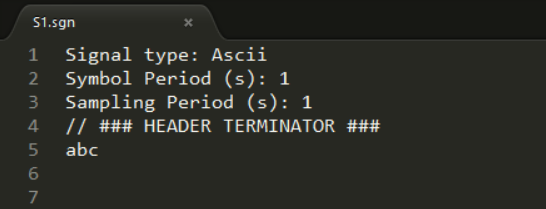
\includegraphics[width=.7\linewidth]{./lib/ascii_to_binary/figures/ascii_signal.png}
\caption{Ascii signal passed as input to the AsciiToBinary block}\label{AsciiSignalImage}
\end{figure}

\begin{figure}[h]
	\centering
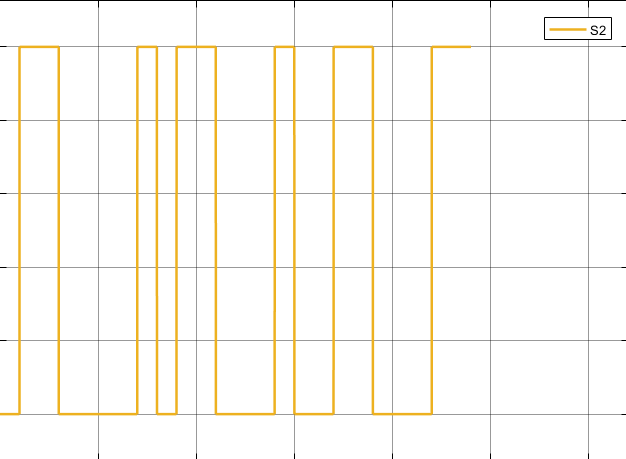
\includegraphics[width=.5\linewidth]{./lib/ascii_to_binary/figures/binary_signal.png}
\caption{Resulting Binary signal from the output of the AsciiToBinary block}\label{BinarySignalImage}
\end{figure}
\pagebreak

\subsection*{Input Signals}

\subparagraph*{Number:} 1

\subparagraph*{Type:} Ascii

\subsection*{Output Signals}

\subparagraph*{Number:} 1

\subparagraph*{Type:} Ascii
\clearpage

\section{Balanced Beam Splitter}

\begin{tcolorbox}	
\begin{tabular}{p{2.75cm} p{0.2cm} p{10.5cm}} 	
\textbf{Header File}   &:& balanced\_beam\_splitter.h \\
\textbf{Source File}   &:& balanced\_beam\_splitter.cpp \\
\textbf{Version}       &:& 20180124
\end{tabular}
\end{tcolorbox}

\subsection*{Input Parameters}

\begin{table}[H]
\centering
\begin{tabular}{|l|l|l|}
\hline
Name           & Type    & Default Value     \\ \hline
Matrix         & array <t\_complex, 4> & $\lbrace~\lbrace \frac{1}{\sqrt{2}},~\frac{1}{\sqrt{2}},~\frac{1}{\sqrt{2}},~\frac{-1}{\sqrt{2}} \rbrace~\rbrace$                             \\ \hline
Mode           & double  & 0                 \\ \hline
\end{tabular}
\end{table}

\subsection*{Functional Description}
The structure of the beam splitter can be controlled with the parameter mode.\\
When \textbf{Mode = 0} the beam splitter will have one input port and two output ports - \textbf{1x2 Beam Splitter}. If Mode has a value different than 0, the splitter will have two input ports and two output ports - \textbf{2x2 Beam Splitter}.\\
Considering the first case, the matrix representing a 2x2 Beam Splitter can be summarized in the following way,

\begin{equation}
M_{BS}=~\frac{\sqrt{2}}{2}\begin{bmatrix}
              					1  & 1 \\
            					1 & -1
            			  \end{bmatrix}
\end{equation}
The relation between the values of the input ports and the values of the output ports can be established in the following way

\begin{equation}
\begin{bmatrix}
A' \\
B'
\end{bmatrix}=M_{BS} \dot{}{\begin{bmatrix}
			  				     A \\
			  	                 B
			  	                 \end{bmatrix}}
\end{equation}
Where, A and B represent the inputs and A' and B' represent the outputs of the Beam Splitter.

\subsection*{Input Signals}

\textbf{Number}: 1 or 2\\
\textbf{Type}: Complex

\subsection*{Output Signals}

\textbf{Number}: 2\\
\textbf{Type}: Complex




%%%%%%%%%%%%%%%%%%%%%%%%%%%%%%%%%%%%%%%%%%%%%%%%%%%%%%%%%%%%%%%%%%%%%%%%%%%%%%%%%%%%%%%%%%%%%%%%%%%%%%%%%%%%
% References
%%%%%%%%%%%%%%%%%%%%%%%%%%%%%%%%%%%%%%%%%%%%%%%%%%%%%%%%%%%%%%%%%%%%%%%%%%%%%%%%%%%%%%%%%%%%%%%%%%%%%%%%%%%%

%\renewcommand{\bibname}{References}
%
%\bibliographystyle{unsrt}
% argument is your BibTeX string definitions and bibliography database(s)
%\bibliography{./lib/balanced_beam_splitter/balanced_beam_splitter}
%
%


\clearpage

\section{Bit Error Rate}
\label{sec:bit_error_rate}
\begin{refsection}

\begin{tcolorbox}	
\begin{tabular}{p{2.75cm} p{0.2cm} p{10.5cm}} 	
\textbf{Header File}    &:& bit\_error\_rate\_*.h \\
\textbf{Source File}    &:& bit\_error\_rate\_*.cpp \\
\textbf{Version}        &:& 20171810 (Daniel Pereira)\\
                        &:& 20181424 (Mariana Ramos)
\end{tabular}
\end{tcolorbox}

\subsection*{Input Parameters}

\begin{table}[H]
\centering
\begin{tabular}{|l|l|l|}
\hline
Name           & Type           & Default Value     \\ \hline
alpha          & double         & 0.05              \\ \hline
m              & integer        & 0                 \\ \hline
lMinorant      & double         & $1\times10^{-10}$ \\ \hline
\end{tabular}
\end{table}


\subsection*{Methods}

\begin{itemize}
  \item BitErrorRate(vector<Signal *> \&InputSig, vector<Signal *> \&OutputSig) :Block(InputSig,OutputSig)\{\};
  \item void initialize(void);
  \item bool runBlock(void);
  \item void setConfidence(double P) \{ alpha = 1-P; \}
  \item void setMidReportSize(int M) \{ m = M; \}
  \item void setLowestMinorant(double lMinorant) \{ lowestMinorant=lMinorant; \}
\end{itemize}




\subsection*{Input Signals}

\textbf{Number}: 2\\
\textbf{Type}: Binary (DiscreteTimeDiscreteAmplitude)


\subsection*{Output Signals}

\textbf{Number}: 1\\
\textbf{Type}: Binary (DiscreteTimeDiscreteAmplitude)

\subsection*{Functional Description}

This block accepts two binary strings and outputs a binary string, outputting a 1 if the two input samples are equal to each other and 0 if not. This block also outputs \textit{.txt} files with a report of the estimated Bit Error Rate (BER), $\widehat{\text{BER}}$ as well as the estimated confidence bounds for a given probability $\alpha$. In version \textbf{20181113} instead of the previous binary output string, this block outputs a 0 if the two input samples are equal and 1 if not.
\par
The block allows for mid-reports to be generated, the number of bits between reports is customizable, if it is set to 0 then the block will only output the final report. In version \textbf{20180424} this block can operate mid-reports using a CUMULATIVE mode, in which the BER is calculated in a cumulative way taking into account all received bits, coincidences and errors, or in a RESET mode, in which at each \textbf{m} bits the number of received bits and coincidence bits is reset for the BER calculation.

\subsection*{Theoretical Description}\label{bercalc}
The $\widehat{\text{BER}}$ is obtained by counting both the total number received bits, $N_T$, and the number of coincidences, $K$, and calculating their relative ratio:
\begin{equation}
\widehat{\text{BER}}=1-\frac{K}{N_T}.
\end{equation}
The upper and lower bounds, $\text{BER}_\text{UB}$ and $\text{BER}_\text{LB}$ respectively, are calculated using the Clopper-Pearson confidence interval, which returns the following simplified expression for $N_T>40$~\cite{Almeida16}:
\begin{align}
\text{BER}_\text{UB}&=\widehat{\text{BER}}+\frac{1}{\sqrt{N_T}}z_{\alpha/2}\sqrt{\widehat{\text{BER}}(1-\widehat{\text{BER}})}+\frac{1}{3N_T}\left[2\left(\frac{1}{2}-\widehat{\text{BER}}\right)z_{\alpha/2}^2+(2-\widehat{\text{BER}})\right]\\
\text{BER}_\text{LB}&=\widehat{\text{BER}}-\frac{1}{\sqrt{N_T}}z_{\alpha/2}\sqrt{\widehat{\text{BER}}(1-\widehat{\text{BER}})}+\frac{1}{3N_T}\left[2\left(\frac{1}{2}-\widehat{\text{BER}}\right)z_{\alpha/2}^2-(1+\widehat{\text{BER}})\right],
\end{align}
where $z_{\alpha/2}$ is the $100\left(1-\frac{\alpha}{2}\right)$th percentile of a standard normal distribution.

\subsection*{Version 20181424}

Version 20181424 allows the user to choose the type of middle reports he wants. So, the input parameter \textrm{mideRepType} can has the value \textit{Cumulative}, where the BER estimation is done by taking into account all samples acquired in a cumulative way, or \textit{Reset}, where the BER estimation is done by taking into account only the number of samples set as \textit{m} in each middle report.

\begin{itemize}
  \item \textbf{Input Parameters}
  \begin{table}[H]
    \centering
    \begin{tabular}{|l|l|l|}
    \hline
    Name           & Type           & Default Value     \\ \hline
    midRepType     & MidReportType  & Cumulative \\ \hline
    \end{tabular}
  \end{table}

  \item \textbf{Methods}
  \begin{itemize}
    \item void setMidReportType(MidReportType mrt) \{ midRepType = mrt; \};
  \end{itemize}
\end{itemize}




% bibliographic references for the section ----------------------------
\clearpage
\printbibliography[heading=subbibliography]
\end{refsection}
\addcontentsline{toc}{subsection}{Bibliography}
\cleardoublepage
% --------------------------------------------------------------------- 
\clearpage

\section{Binary source}

\maketitle
This block generates a sequence of binary values (1 or 0) and it can work in four different modes: 

\begin{multicols}{2}
\begin{enumerate}
	\item Random
	\item PseudoRandom 
	\item DeterministicCyclic 
	\item DeterministicAppendZeros 
\end{enumerate}
\end{multicols}

This blocks doesn't accept any input signal. It produces any number of output signals.

\subsection*{Input Parameters}

	\begin{itemize}
		\item mode\{PseudoRandom\}\linebreak
		(Random, PseudoRandom, DeterministicCyclic, DeterministicAppendZeros)
		\item probabilityOfZero\{0.5\}\linebreak
		(real $\in$ [0,1])
		\item patternLength\{7\} \linebreak
		(integer $\in$ [1,32]) 
		\item bitStream\{"0100011101010101"\} \linebreak
		(string of 0's and 1's)
		\item numberOfBits\{-1\} \linebreak
		(long int)
		\item bitPeriod\{1.0/100e9\} \linebreak
		(double)
	\end{itemize}

\subsection*{Methods}

BinarySource(vector$\langle$Signal *$\rangle$ \&InputSig, vector$\langle$Signal *$\rangle$ \&OutputSig) :Block(InputSig, OutputSig)\{\};
\bigbreak	 
void initialize(void);
\bigbreak	 
bool runBlock(void);
\bigbreak	 
void setMode(BinarySourceMode m)
BinarySourceMode const getMode(void)
\bigbreak	 
void setProbabilityOfZero(double pZero) 
\bigbreak
double const getProbabilityOfZero(void) 
\bigbreak	 
void setBitStream(string bStream) 
\bigbreak
string const getBitStream(void) 
\bigbreak	 
void setNumberOfBits(long int nOfBits)
\bigbreak
long int const getNumberOfBits(void) 
\bigbreak	 
void setPatternLength(int pLength) 
\bigbreak
int const getPatternLength(void) 
\bigbreak	 
void setBitPeriod(double bPeriod)
\bigbreak
double const getBitPeriod(void) 

\subsection*{Functional description}

The \textit{mode} parameter allows the user to select between one of the four operation modes of the binary source.

\subparagraph*{Random Mode}
Generates a 0 with probability \textit{probabilityOfZero} and a 1 with probability 1-\textit{probabilityOfZero}.

\subparagraph*{Pseudorandom Mode} 
Generates a pseudorandom sequence with period $2^\textit{patternLength}-1$.

\subparagraph*{DeterministicCyclic Mode}
Generates the sequence of 0's and 1's specified by \textit{bitStream} and then repeats it.

\subparagraph*{DeterministicAppendZeros Mode}
Generates the sequence of 0's and 1's specified by \textit{bitStream} and then it fills the rest of the buffer space with zeros.

\subsection*{Input Signals}


\subparagraph*{Number:} 0

\subparagraph*{Type:} Binary (DiscreteTimeDiscreteAmplitude)

\subsection*{Output Signals}

\subparagraph*{Number:} 1 or more

\subparagraph*{Type:} Binary (DiscreteTimeDiscreteAmplitude)

\subsection*{Examples} 

\paragraph*{Random Mode}

\paragraph*{PseudoRandom Mode}
As an example consider a pseudorandom sequence with \textit{patternLength}=3 which contains a total of 7 ($2^3-1$) bits. In this sequence it is possible to find every combination of 0's and 1's that compose a 3 bit long subsequence with the exception of $000$. For this example the possible subsequences are $010$, $110$, $101$, $100$, $111$, $001$ and $100$ (they appear in figure \ref{BinarySequenceN3} numbered in this order). Some of these require wrap. 

\begin{figure}[h]
	\centering
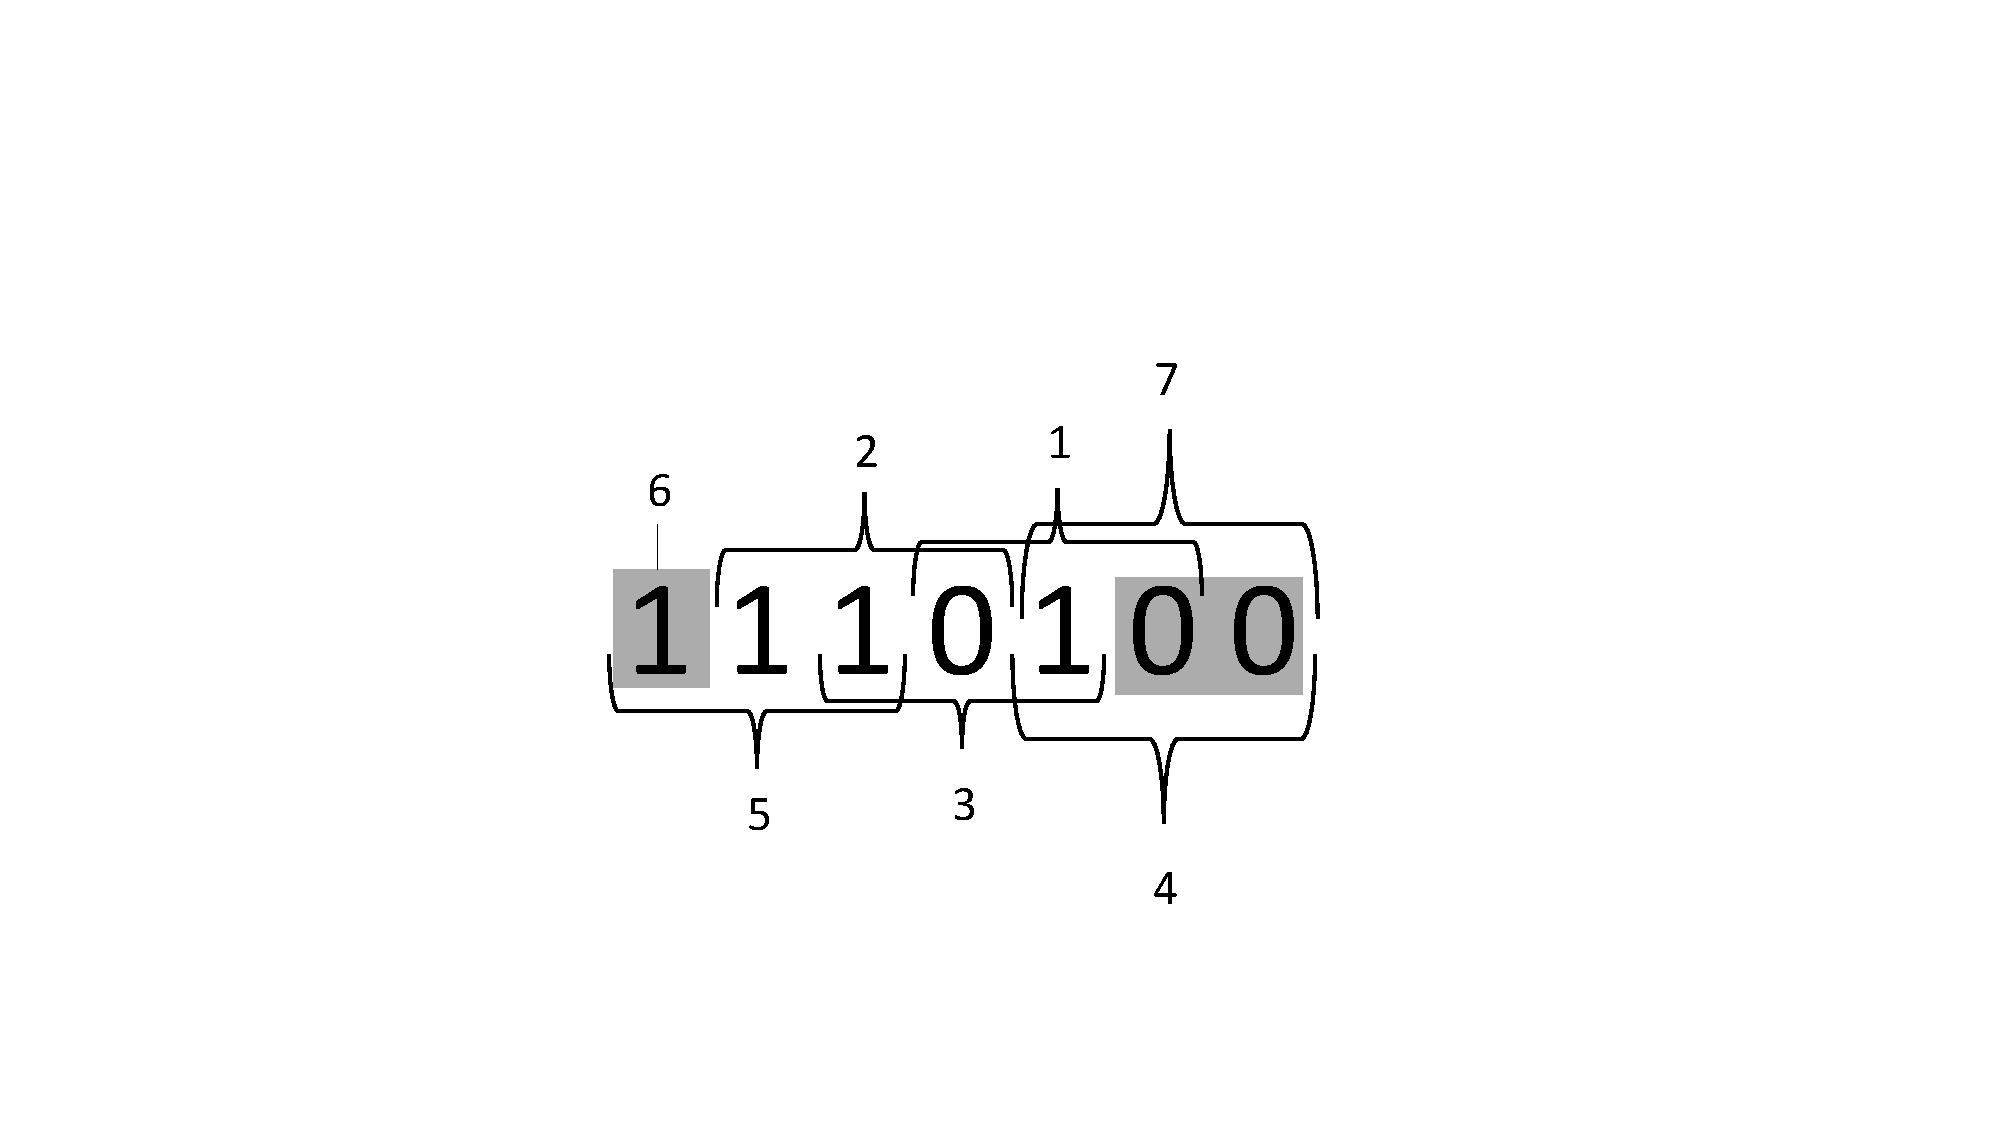
\includegraphics[width=0.5\textwidth]{../m_qam_transmitter/figures/BinarySequenceN3}
\caption{Example of a pseudorandom sequence with a pattern length equal to 3.}\label{BinarySequenceN3}
\end{figure}

\paragraph*{DeterministicCyclic Mode}

As an example take the \textit{bit stream} '0100011101010101'. The generated binary signal is displayed in.

\paragraph*{DeterministicAppendZeros Mode}

Take as an example the \textit{bit stream} '0100011101010101'. The generated binary signal is displayed in \ref{MQAM1_DeterministAppendZeros}.

\begin{figure}
	\centering
	\includegraphics[width=\textwidth]{../m_qam_transmitter/figures/BinarySource_output}
	
	\caption{Binary signal generated by the block operating in the \textit{Deterministic Append Zeros} mode with a binary sequence 01000...}\label{MQAM1_DeterministAppendZeros}
\end{figure}

\subsection*{Sugestions for future improvement}

Implement an input signal that can work as trigger.


\clearpage

\section{Binary To Ascii}

\begin{tcolorbox}	
	\begin{tabular}{p{2.75cm} p{0.2cm} p{10.5cm}} 	
		\textbf{Header File}   &:& binary\_to\_ascii\_*.h \\
		\textbf{Source File}   &:& binary\_to\_ascii\_*.cpp \\
        \textbf{Version}       &:& 20180905 (Andr\'e Mourato)
	\end{tabular}
\end{tcolorbox}

\subsection*{Methods}

BinaryToAscii(vector$\langle$Signal *$\rangle$ \&InputSig, vector$\langle$Signal *$\rangle$ \&OutputSig) :Block(InputSig, OutputSig)\{\};
\bigbreak
void initialize(void);
\bigbreak
bool runBlock(void);
\bigbreak

\subsection*{Functional description}

Figure \ref{BinarySignalImage} shows an example of an input signal that can be passed as argument. This signal contains the binary representation of three characters: a, b and c. Each character can be represented by 8 bits, according to the Ascii Table. This signal contains the following stream of bits: $0110000111000101100011$. There are 24 bits in this stream, therefore we can divide it into three segments of 8 bits each. The resulting segments are: $01100001$, $1100010$ and $1100011$. Each of these segments is the binary code of a character. $01100001$ represents the character $a$, $1100010$ represents the character $b$ and $1100011$ represents the character $c$.
The block BinaryToAscii will convert the binary codes into the respective characters. The resulting output signal will be of type Ascii. The output signal to this example, shown in figure \ref{AsciiSignalImage}, contains the characters that can be represented with the previous binary codes.

\begin{figure}[h]
	\centering
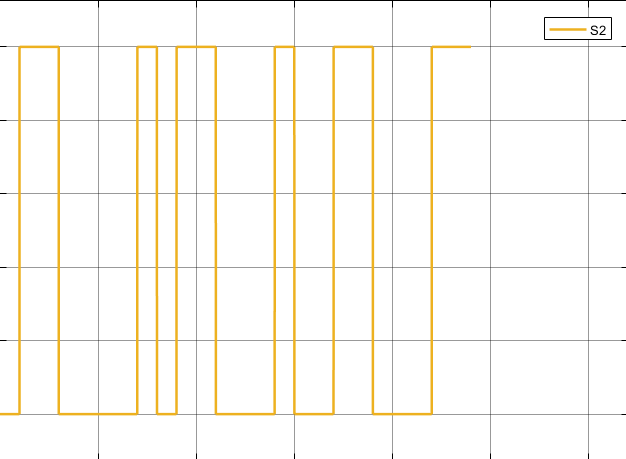
\includegraphics[width=.5\linewidth]{./lib/ascii_to_binary/figures/binary_signal.png}
\caption{Binary signal passed as input to the BinaryToAscii block}\label{BinarySignalImage}
\end{figure}

\begin{figure}[h]
	\centering
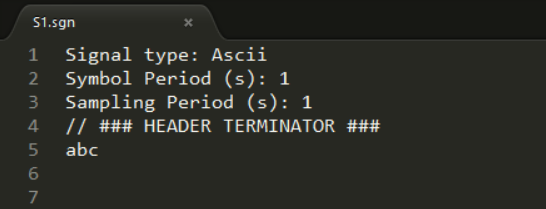
\includegraphics[width=.7\linewidth]{./lib/ascii_to_binary/figures/ascii_signal.png}
\caption{Resulting Ascii signal from the output of the BinaryToAscii block}\label{AsciiSignalImage}
\end{figure}

\pagebreak

\subsection*{Input Signals}

\subparagraph*{Number:} 1

\subparagraph*{Type:} Ascii

\subsection*{Output Signals}

\subparagraph*{Number:} 1

\subparagraph*{Type:} Ascii 
\clearpage

\section{Bob QKD}

\maketitle
This block is the processor for Bob does all tasks that she needs. This block accepts and produces:

\begin{enumerate}
  \item 
  \item 
\end{enumerate}


\subsection*{Input Parameters}

	\begin{itemize}
		\item
		\item
		
	\end{itemize}

\subsection*{Methods}



\subsection*{Functional description}



\subsection*{Input Signals}


\subsection*{Examples}


\subsection*{Sugestions for future improvement} 
\documentclass[../../sdf/tex/BPSK_system.tex]{subfiles}
\graphicspath{{../../images/}}
%opening
\onlyinsubfile{\title{Bit Decider}}
\date{ }

\begin{document}

\onlyinsubfile{\maketitle}

\subsection*{Input Parameters}

\begin{multicols}{2}
	\begin{itemize}
		\item setPosReferenceValue
		\item setNegReferenceValue
	\end{itemize}
\end{multicols}

\subsection*{Functional Description}

This block accepts one real discrete signal and outputs a binary string, outputting a 1 if the input sample is above the predetermined reference level and 0 if it is below another reference value The reference values are defined by the values of \textit{PosReferenceValue} and \textit{NegReferenceValue}.

\subsection*{Input Signals}

\textbf{Number}: 1

\textbf{Type}: Real signal (DiscreteTimeContinuousAmplitude)

\subsection*{Output Signals}

\textbf{Number}: 1

\textbf{Type}: Binary (DiscreteTimeDiscreteAmplitude)


\end{document}
\clearpage

\section{Clock}

\begin{tcolorbox}	
	\begin{tabular}{p{2.75cm} p{0.2cm} p{10.5cm}} 	
		\textbf{Header File}   &:& clock.h \\
		\textbf{Source File}   &:& clock.cpp \\
	\end{tabular}
\end{tcolorbox}

This block doesn't accept any input signal. It outputs one signal that corresponds to a sequence of Dirac's delta functions with a user defined \textit{period}.

\subsection*{Input Parameters}

%\begin{itemize}
%	\item period\{ 0.0 \};
%	\item samplingPeriod\{ 0.0 \};
%\end{itemize}

\begin{table}[h]
	\centering
	\begin{tabular}{|c|c|c|c|cccc}
		\cline{1-4}
		\textbf{Parameter} & \textbf{Type} & \textbf{Values} &   \textbf{Default}& \\ \cline{1-4}
		period & double & any & $0.0$ \\ \cline{1-4}
		samplingPeriod & double & any & $0.0$ \\ \cline{1-4}
	\end{tabular}
	\caption{Binary source input parameters}
	\label{table:clock_in_par}
\end{table}

\subsection*{Methods}

Clock() {}
\bigbreak
Clock(vector$<$Signal *$>$ \&InputSig, vector$<$Signal *$>$ \&OutputSig) :Block(InputSig, OutputSig) {}
\bigbreak
void initialize(void)
\bigbreak
bool runBlock(void)
\bigbreak
void setClockPeriod(double per)
\bigbreak
void setSamplingPeriod(double sPeriod)

\subsection*{Functional description}


\pagebreak

\subsection*{Input Signals}

\subparagraph*{Number:} 0

\subsection*{Output Signals}

\subparagraph*{Number:} 1

\subparagraph*{Type:} Sequence of Dirac's delta functions. (TimeContinuousAmplitudeContinuousReal)

\subsection*{Examples}

%\begin{figure}[h]
%	\centering
%	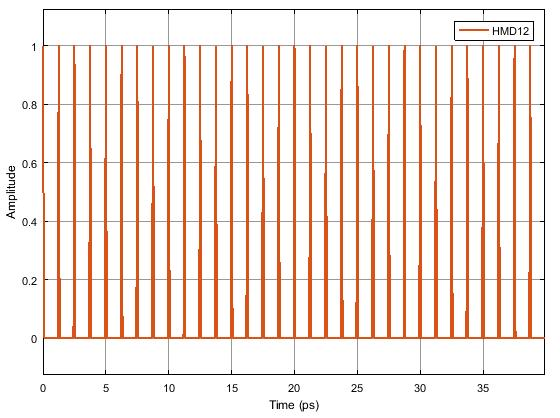
\includegraphics[width=\textwidth]{./lib/clock/figures/Clock_output}
%	\caption{Example of the output signal of the clock}\label{Clock_output}
%\end{figure}

\subsection*{Sugestions for future improvement}


\clearpage

\section{Clock\_20171219}

This block doesn't accept any input signal. It outputs one signal that corresponds to a sequence of Dirac's delta functions with a user defined \textit{period}, \textit{phase} and \textit{sampling period}.

\subsection*{Input Parameters}

\begin{itemize}
	\item period\{ 0.0 \};
	\item samplingPeriod\{ 0.0 \};
    \item phase \{0.0\};
\end{itemize}

\subsection*{Methods}

Clock() {}
\bigbreak
Clock(vector$<$Signal *$>$ \&InputSig, vector$<$Signal *$>$ \&OutputSig) :Block(InputSig, OutputSig) {}
\bigbreak
void initialize(void)
\bigbreak
bool runBlock(void)
\bigbreak
void setClockPeriod(double per)
double getClockPeriod()
\bigbreak
void setClockPhase(double pha)
double getClockPhase()
\bigbreak
void setSamplingPeriod(double sPeriod)
double getSamplingPeriod()

\subsection*{Functional description}


\subsection*{Input Signals}

\subparagraph*{Number:} 0

\subsection*{Output Signals}

\subparagraph*{Number:} 1

\subparagraph*{Type:} Sequence of Dirac's delta functions. (TimeContinuousAmplitudeContinuousReal)

\subsection*{Examples}

\begin{figure}[h]
	\centering
	\includegraphics[width=\textwidth]{./lib/clock_20171219/figures/clock_withoutpha}
	\caption{Example of the output signal of the clock without phase shift.}
\end{figure}

\begin{figure}[h]
	\centering
	\includegraphics[width=\textwidth]{./lib/clock_20171219/figures/clockPhased}
	\caption{Example of the output signal of the clock with phase shift.}
\end{figure}

\subsection*{Sugestions for future improvement}


\clearpage

\section{Complex To Real}

\begin{tcolorbox}	
	\begin{tabular}{p{2.75cm} p{0.2cm} p{10.5cm}} 	
		\textbf{Header File}   &:& complex\_to\_real$\_*$.h \\
		\textbf{Source File}   &:& complex\_to\_real$\_*$.cpp \\
        \textbf{Version}       &:& 20180717 (Celestino Martins) \\
	\end{tabular}
\end{tcolorbox}

This super block converts a complex input signal into two real signals.

\subsection*{Input Parameters}



\subsection*{Methods}

\begin{itemize}
  \item ComplexToReal() \{\};
  \item ComplexToReal(vector<Signal *> \&InputSig, vector<Signal *> \&OutputSig) :Block(InputSig,OutputSig)\{\};
  \item void initialize(void);
  \item bool runBlock(void);
\end{itemize}

\subsection*{Functional description}

This super block converts a complex input signal into two real signals.


\pagebreak
\subsection*{Input Signals}

\subparagraph*{Number:} 1

\subsection*{Output Signals}

\subparagraph*{Number:} 2

\subparagraph*{Type:} Electrical complex signal

\subsection*{Examples}

\subsection*{Sugestions for future improvement}



\clearpage
\section{Coupler 2 by 2}

In general, the matrix representing 2x2 coupler can be summarized in the following way,
\begin{equation}
\begin{bmatrix}
A' \\
B'
\end{bmatrix}=\begin{bmatrix}
  					T  & iR \\
					iR & T
			  \end{bmatrix} \dot{}{\begin{bmatrix}
			  				     A \\
			  	                 B
			  	                 \end{bmatrix}}
\end{equation}
Where, A and B represent inputs to the 2x2 coupler and A' and B' represent output of the 2x2 coupler. Parameters T and R represent transmitted and reflected part respectively which can be quantified in the following form,

\begin{equation}
T=\sqrt{1-\eta_{R}}
\end{equation}

\begin{equation}
R=\sqrt{\eta_{R}}
\end{equation}
Where, value of the $\sqrt{\eta_{R}}$ lies in the range of $0 \leq \sqrt{\eta_{R}} \leq 1$.
\begin{figure}
	\centering
	\includegraphics[width=\textwidth]{./lib/coupler_2_by_2/figures/coupler_2_by_2.pdf}
	\caption{2x2 coupler}\label{}
\end{figure}

It is worth to mention that if we put $\eta_{R}=1/2$ then it leads to a special case of "Balanced Beam splitter" which equally distribute the input power into both output ports.

\clearpage

\section{Carrier Phase Compensation}

\begin{tcolorbox}	
	\begin{tabular}{p{2.75cm} p{0.2cm} p{10.5cm}} 	
		\textbf{Header File}   &:& carrier\_phase\_estimation$\_*$.h \\
		\textbf{Source File}   &:& carrier\_phase\_estimation$\_*$.cpp \\
        \textbf{Version}       &:& 20180423 (Celestino Martins) \\
	\end{tabular}
\end{tcolorbox}

This block performs the laser phase noise compensation using either Viterbi-Viterbi (VV) algorithm or blind phase search algorithm (BPS). For both cases, it receives one input complex signal and outputs one complex signal.

\subsection*{Input Parameters For VV Algorithms}

\begin{table}[h]
	\centering
	\begin{tabular}{|c|c|c|c|cccc}
		\cline{1-4}
		\textbf{Parameter} & \textbf{Type} & \textbf{Values} &   \textbf{Default}& \\ \cline{1-4}
		nTaps              & int & any & $25$ \\ \cline{1-4}
        methodType         & string & VV & VV \\ \cline{1-4}
		mQAM                  & int & any & $4$ \\ \cline{1-4}		
	\end{tabular}
	\caption{CPE input parameters}
	\label{table:cpe_in_par_vv}
\end{table}


\subsection*{Input Parameters For BPS Algorithms}

\begin{table}[h]
	\centering
	\begin{tabular}{|c|c|c|c|cccc}
		\cline{1-4}
		\textbf{Parameter} & \textbf{Type} & \textbf{Values} &   \textbf{Default}& \\ \cline{1-4}
		nTaps              & int & any & $25$ \\ \cline{1-4}
        NtestPhase         & int & any & $32$ \\ \cline{1-4}
        methodType         & string & BPS & VV \\ \cline{1-4}
		mQAM                  & int & any & $4$ \\ \cline{1-4}	
	\end{tabular}
	\caption{CPE input parameters}
	\label{table:cpe_in_par_bps}
\end{table}

\subsection*{Methods}

CarrierPhaseCompensation() {};
\bigbreak
CarrierPhaseCompensation(vector$<$Signal *$>$ \&InputSig, vector$<$Signal *$>$ \&OutputSig) :Block(InputSig, OutputSig)\{\};
\bigbreak
void initialize(void);
\bigbreak
bool runBlock(void);
\bigbreak
void setnTaps(int ntaps) { nTaps = ntaps; }
\bigbreak
double getnTaps() { return nTaps; }
\bigbreak
void setmQAM(int mQAMs) { mQAM = mQAMs; }
\bigbreak
double getmQAM() { return mQAM; }
\bigbreak
void setTestPhase(int nTphase) { nTestPhase = nTphase; }
\bigbreak
double getTestPhase() { return nTestPhase; }
\bigbreak
void setmethodType(string mType) { methodType = mType; }
\bigbreak
string getmethodType() { return methodType; }
\bigbreak
void setBPStype(string tBPS) { BPStype = tBPS; }
\bigbreak
string getBPStype() { return BPStype; }

\subsection*{Functional description}

This block can perform the carrier phase noise compensation originated by the laser source and local oscillator in coherent optical communication systems. For the sake of simplicity, in this simulation we have restricted all the phase noise at the transmitter side, in this case generated by the laser source, which is then compensated at the receiver side using DSP algorithms.
In this simulation, the carrier phase noise compensation can be performed by applying either the well known Viterbi-Viterbi (VV) algorithm or blind phase search algorithm (BPS), by configuring the parameter $methodType$. The parameter $methodType$ is defined as a string type and it can be configured as: i) When the parameter $methodType$ is $\textit{VV}$ it is applied the VV algorithm; When the parameter $methodType$ is $\textit{BPS}$ it is applied the BPS algorithm.

\subsubsection{Viterbi-Viterbi Algorithm}
\begin{figure}[h!]
    \centering
    \includegraphics[width=\textwidth]{./lib/carrier_phase_estimation/figures/VV_phaseEstimation.pdf}
    \caption{Block diagram of Viterbi-Viterbi algorithm for carrier phase recovery.}
    \label{fig_VVdiagram}
\end{figure}
VV algorithm is a n-th power feed-forward approach employed for uniform angular distribution characteristic of m-PSK constellations, where the information of the modulated phase is removed by employing the n-th power operation on the received symbols. The algorithm implementation diagram is shown in Figure~\ref{fig_VVdiagram}, starting with M-th power operation on the received symbols. In order to minimize the impact of additive noise in the estimation process, a sum of $2N+1$ symbols is considered, which is then divided by M. The resulting estimated phase noise is then submitted to a phase unwrap function in order to avoid the occurrence of cycle slip. The final phase noise estimator is then used to compensate for the phase noise of the original symbol in the middle of the symbols block.

\subsubsection{Blind Phase Search Algorithm}
\begin{figure}[h!]
    \centering
    \includegraphics[width=12cm]{./lib/carrier_phase_estimation/figures/bps_diagram.pdf}
    \caption{Block diagram of blind phase search algorithm for carrier phase recovery.}
    \label{fig_BPSdiagram}
\end{figure}
An alternative to the VV phase noise estimator is the so-called BPS algorithm, in which the operation principle is shown in the Figure~\ref{fig_BPSdiagram}. Firstly, a block of $2N+1$ consecutive received symbols is rotated by a number of $B$ uniformly distributed test phases defined as,
\begin{equation}
    	\phi_{b} = \frac{b}{B}\frac{\pi}{2}, b \in\{0,1,...,B-1\}.
    \label{eq_phaseNoise}
\end{equation}
Then, the rotated blocks symbols are fed into decision circuit, where the square distance to the closest constellation points in the original constellation is calculated for each block. Each resulting square distances block is summed up to minimize the noise distortion. After average filtering, the test phase providing the minimum sum of distances is considered to be the phase noise estimator for the symbol in the middle of the block. The estimated phase noise is then unwrapped to reduce cycle slip occurrence, which is then used employed for the compensation for the phase noise of the original symbols.

\pagebreak
\subsection*{Input Signals}

\subparagraph*{Number:} 1

\subsection*{Output Signals}

\subparagraph*{Number:} 1

\subparagraph*{Type:} Electrical complex signal

\subsection*{Examples}

\subsection*{Sugestions for future improvement}



\clearpage

\section{Decision Circuit}

\begin{tcolorbox}	
	\begin{tabular}{p{2.75cm} p{0.2cm} p{10.5cm}} 	
		\textbf{Header File}   &:& decision\_circuit$\_*$.h \\
		\textbf{Source File}   &:& decision\_circuit$\_*$.cpp \\
        \textbf{Version}       &:& 20181012 (Celestino Martins) \\
	\end{tabular}
\end{tcolorbox}

This block performs the symbols decision, by calculating the minimum distance between the received symbol relatively to the constellation map. It receives one input complex signal and outputs one complex signal.

\subsection*{Input Parameters}

\begin{table}[h]
	\centering
	\begin{tabular}{|c|c|c|c|cccc}
		\cline{1-4}
		\textbf{Parameter} & \textbf{Type} & \textbf{Values} &   \textbf{Default}& \\ \cline{1-4}
		mQAM                  & int & any & $4$ \\ \cline{1-4}		
	\end{tabular}
	\caption{Decision circuit input parameters}
	\label{table:cpe_in_par_vv}
\end{table}


\subsection*{Methods}

DecisionCircuitMQAM() {};
\bigbreak
DecisionCircuitMQAM(vector$<$Signal *$>$ \&InputSig, vector$<$Signal *$>$ \&OutputSig) :Block(InputSig, OutputSig)\{\};
\bigbreak
void initialize(void);
\bigbreak
bool runBlock(void);
\bigbreak
void setmQAM(int mQAMs) { mQAM = mQAMs; }
\bigbreak
double getmQAM() { return mQAM; }

\subsection*{Functional description}

This block performs the symbols decision, by minimizing the distance between the received symbol relatively to the constellation map. It perform the symbol decision for the modulations formats, 4QAM and 16QAM. The order of modulation format is defined by the parameter $mQAM$.

\pagebreak
\subsection*{Input Signals}

\subparagraph*{Number:} 1

\subsection*{Output Signals}

\subparagraph*{Number:} 1

\subparagraph*{Type:} Electrical complex signal

\subsection*{Examples}

\subsection*{Sugestions for future improvement}
Extend the decision to higher order modulation format.


\clearpage

\section{Decoder}

This block accepts a complex electrical signal and outputs a sequence of binary values (0's and 1's). Each point of the input signal corresponds to a pair of bits.

\subsection*{Input Parameters}

\begin{itemize}
	\item\texttt{t\_integer} m\{ 4 \}
	\item vector$<$\texttt{t\_complex}$>$ iqAmplitudes\{ \{ 1.0, 1.0 \},\{ -1.0, 1.0 \},\{ -1.0, -1.0 \},\{ 1.0, -1.0 \} \};
\end{itemize}

\subsection*{Methods}
 
Decoder() {}
\bigbreak
Decoder(vector$<$Signal *$>$ \&InputSig, vector$<$Signal *$>$ \&OutputSig) :Block(InputSig, OutputSig) {}
\bigbreak
void initialize(void)
\bigbreak
bool runBlock(void)
\bigbreak
void setM(int mValue)
\bigbreak
void getM()
\bigbreak
void setIqAmplitudes(vector$<$\texttt{t\_iqValues}$>$ iqAmplitudesValues)
\bigbreak
vector$<$\texttt{t\_iqValues}$>$getIqAmplitudes()

\subsection*{Functional description}

This block makes the correspondence between a complex electrical signal and pair of binary values using a predetermined constellation.

To do so it computes the distance in the complex plane between each value of the input signal and each value of the \textit{iqAmplitudes} vector selecting only the shortest one. It then converts the point in the IQ plane to a pair of bits making the correspondence between the input signal and a pair of bits.

\pagebreak

\subsection*{Input Signals}

\subparagraph*{Number:} 1

\subparagraph*{Type:} Electrical complex (TimeContinuousAmplitudeContinuousReal)

\subsection*{Output Signals}

\subparagraph*{Number:} 1

\subparagraph*{Type:} Binary 

\subsection*{Examples}

As an example take an input signal with positive real and imaginary parts. It would correspond to the first point of the \textit{iqAmplitudes} vector and therefore it would be associated to the  pair of bits $00$. 

\begin{figure}[h]
	\centering
	\includegraphics[width=\textwidth]{../homodyne_receiver/figures/Decoder_output}
	\caption{Example of the output signal of the decoder for a binary sequence 01. As expected it reproduces the initial bit stream}\label{Decoder_output}
\end{figure}

\subsection*{Sugestions for future improvement}

\documentclass[a4paper]{article}
\usepackage[top=1in, bottom=1.25in, left=1.25in, right=1.25in]{geometry}
\usepackage{amsmath}
\usepackage{multicol}
\usepackage{graphicx}
\RequirePackage{ltxcmds}[2010/12/07]
%opening
\title{Discrete to Continuous Time}


\begin{document}

\maketitle

This block converts a signal from a discrete time signal to a continuous time signal. To do so it reads the input signal buffer value, puts it in the output signal buffer and it fills the rest of the space available for thar symbol with zeros.

\subsection*{Input Parameters}

\begin{itemize}
	\item numberOfSamplesPerSymbol 
\end{itemize}

\subsection*{Functional Description}

\subsection*{Input Signals}

\textbf{Number}: 1

\textbf{Type}: Sequence of 1's and -1's. (DiscreteTimeDiscreteAmplitude)

\subsection*{Output Signals}

\textbf{Number}: 2

\textbf{Type}: Sequence of Dirac Delta functions (ContinuousTimeDiscreteAmplitude)

\subsection*{Example}

\begin{figure}[h]
	\includegraphics[width=\textwidth]{MQAM4}
\end{figure}

\subsection*{Sugestions for future improvement}

\pagebreak



\end{document}
\clearpage

\section{DownSampling}

\begin{tcolorbox}	
	\begin{tabular}{p{2.75cm} p{0.2cm} p{10.5cm}} 	
		\textbf{Header File}   &:& down\_sampling$\_*$.h \\
		\textbf{Source File}   &:& down\_sampling$\_*$.cpp \\
        \textbf{Version}       &:& 20180917 (Celestino Martins) \\
	\end{tabular}
\end{tcolorbox}

This block simulates the down-sampling function, where the signal sample rate is decreased by integer factor.

\subsection*{Input Parameters}

\begin{table}[h]
	\centering
	\begin{tabular}{|c|c|c|c|cccc}
		\cline{1-4}
		\textbf{Parameter} & \textbf{Type} & \textbf{Values} &   \textbf{Default}& \\ \cline{1-4}
		downSamplingFactor & int & any & $2$ \\ \cline{1-4}	
	\end{tabular}
	\caption{DownSampling input parameters}
	\label{table:down_sampling}
\end{table}


\subsection*{Methods}

DownSampling() {};
\bigbreak
DownSampling(vector$<$Signal *$>$ \&InputSig, vector$<$Signal *$>$ \&OutputSig) :Block(InputSig, OutputSig)\{\};
\bigbreak
void initialize(void);
\bigbreak
bool runBlock(void);
\bigbreak
void setSamplingFactor(unsigned int dSamplingfactor) { downSamplingFactor = dSamplingfactor; }
\bigbreak
unsigned int getSamplingFactor() { return downSamplingFactor; }

\subsection*{Functional description}

This block perform decreases the sample rate of input signal by a factor of $downSamplingFactor$. Given a down-sampling factor, $downSamplingFactor$, the output signal correspond to the first sample of input signal and every $downSamplingFactor^{th}$ sample after the first.


\pagebreak
\subsection*{Input Signals}

\subparagraph*{Number:} 1

\subsection*{Output Signals}

\subparagraph*{Number:} 1

\subparagraph*{Type:} Electrical real signal

\subsection*{Examples}

\subsection*{Sugestions for future improvement}



\clearpage

\section{DSP}

\begin{tcolorbox}	
	\begin{tabular}{p{2.75cm} p{0.2cm} p{10.5cm}} 	
		\textbf{Header File}   &:& dsp$\_*$.h \\
		\textbf{Source File}   &:& dsp$\_*$.cpp \\
        \textbf{Version}       &:& 20180423 (Celestino Martins) \\
	\end{tabular}
\end{tcolorbox}

This super block simulates the digital signal processing (DSP) algorithms for system impairments compensation in digital domain. It includes the real to complex block, carrier phase recovery block (CPE) and complex to real block. It receives two real input signal and outputs two real signal.

\subsection*{Input Parameters}

\begin{table}[h]
	\centering
	\begin{tabular}{|c|c|c|c|cccc}
		\cline{1-4}
		\textbf{Parameter} & \textbf{Type} & \textbf{Values} &   \textbf{Default}& \\ \cline{1-4}
		nTaps              & int & any & $25$ \\ \cline{1-4}
        NtestPhase         & int & any & $32$ \\ \cline{1-4}
        methodType         & int & any & $[0,1]$ \\ \cline{1-4}
		samplingPeriod     & double & any & $0.0$ \\ \cline{1-4}	
	\end{tabular}
	\caption{DSP input parameters}
	\label{table:dsp_in_par}
\end{table}

\subsection*{Methods}

DSP(vector$<$Signal *$>$ \&InputSig, vector$<$Signal *$>$ \&OutputSig);
\bigbreak
void setCPEnTaps(double nTaps) { B02.setnTaps(nTaps); }
\bigbreak
void setCPETestPhase(double TestPhase) { B02.setTestPhase(TestPhase); }
\bigbreak
void setCPESamplingPeriod(double sPeriod) { B02.setSamplingPeriod(sPeriod); }
\bigbreak
void setCPEmethodType(string mType) { B02.setmethodType(mType); }
\bigbreak
void setSamplingPeriod(double sPeriod) { B02.setSamplingPeriod(sPeriod); };

\subsection*{Functional description}

This super block is composed of three blocks, real to complex block, carrier phase recovery block and complex to real block. The two real input signals are combined into a complex signal using real to complex block. The obtained complex signal is then fed to the CPE block, where the laser phase noise compensation is performed. Finally, the complex output of CPE block is converted into two real signal using complex to real block. 


\pagebreak
\subsection*{Input Signals}

\subparagraph*{Number:} 2

\subsection*{Output Signals}

\subparagraph*{Number:} 2

\subparagraph*{Type:} Electrical complex signal

\subsection*{Examples}

\subsection*{Sugestions for future improvement}



\clearpage

\section{EDFA}

\begin{tcolorbox}	
	\begin{tabular}{p{2.75cm} p{0.2cm} p{10.5cm}} 	
		\textbf{Header File}   &:& m\_qam\_receiver.h \\
		\textbf{Source File}   &:& m\_qam\_receiver.cpp \\
	\end{tabular}
\end{tcolorbox}

This block mimics  an EDFA in the simplest way, by accepting one optical input
signal and outputting an amplified version of that signal, affected by white
noise.

\begin{figure}[h]
	\centering
	\includegraphics[width=0.5\textwidth]{./lib/edfa/figures/edfa_simple}
	\caption{Basic configuration of the MQAM
	receiver}\label{fig:edfa_simple}
\end{figure}

\subsection*{Functional description}

This block of code simulates the basic functionality of an EDFA: it amplifies
the optical signal by a given gain, and adds noise according to a certain noise
figure. Currently the only parameters are the gain and noise figure, and it's
assumed that the output power is always far below the EDFA's saturation
power. Therefore, the gain and noise spectral density are independent of the
signal. The noise spectral density is calculated from the noise
figure, gain and wavelength.

This block is made of smaller blocks, and its internal constitution is shown in
Figure~\ref{fig:edfa_blocks}.

\begin{figure}[h]
	\centering
	\includegraphics[width=0.7\textwidth]{./lib/edfa/figures/edfa_blocks}
	\caption{Schematic representation of the block homodyne
	receiver.}\label{fig:edfa_blocks}
\end{figure}

\subsection*{Input parameters}

%This block has some input parameters that can be manipulated by the user in
%order oto change the basic configuration of the receiver. Each parameter has
%associated a function that allows for its change. In the following table
%(table~\ref{table}) the input parameters and corresponding functions are
%summarized.
%
\begin{table}[h]
	\begin{center}
		\begin{tabular}{| m{3,2cm} | m{6,2cm} |  m{2,2cm} | m{4cm} | }
			\hline
			\textbf{Input parameters} & \textbf{Function} & \textbf{Type} \\\hline
			powerGain\_dB             & setGain\_dB       & t\_real       \\\hline
			noiseFigure               & setNoiseFigure    & t\_real       \\\hline
			samplingPeriod            & setNoiseFigure    & t\_real       \\\hline
			wavelength                & setWavelength     & t\_real       \\\hline
			dirName                   & setDirName        & string        \\\hline
		\end{tabular}
		\caption{List of input parameters of the EDFA block} \label{table}
	\end{center}
\end{table}
%
\pagebreak

\subsection*{Methods}

Edfa(vector<Signal *> \&inputSignal, vector<Signal *> \&outputSignal);
(\textbf{constructor})0
\bigbreak
void setGain\_dB(t\_real newGain)
\bigbreak
t\_real getGain\_dB(void)
\bigbreak
void setNoiseFigure(t\_real newNoiseFigure)
\bigbreak
t\_real getNoiseFigure(void)
\bigbreak
void setNoiseSamplingPeriod(t\_real newSamplingPeriod)
\bigbreak
t\_real getNoiseSamplingPeriod(void)
\bigbreak
void setWavelength(t\_real newWavelength)
\bigbreak
t\_real getNoiseFigure(void)
\bigbreak
void setDirName(string newDirName);
\bigbreak
string getDirName(void)
\bigbreak
%HomodyneReceiver(vector$<$Signal *$>$ \&inputSignal, vector$<$Signal *$>$
%\&outputSignal)
%\bigbreak
%void setIqAmplitudes(vector$<$t\_iqValues$>$ iqAmplitudesValues)
%\bigbreak
%vector$<$t\_iqValues$>$ const getIqAmplitudes(void)
%\bigbreak
%void setLocalOscillatorSamplingPeriod(double sPeriod)
%\bigbreak
%void setLocalOscillatorOpticalPower(double opticalPower)
%\bigbreak
%void setLocalOscillatorOpticalPower\_dBm(double opticalPower\_dBm)
%\bigbreak
%void setLocalOscillatorPhase(double lOscillatorPhase)
%\bigbreak
%void setLocalOscillatorOpticalWavelength(double lOscillatorWavelength)
%\bigbreak
%void setSamplingPeriod(double sPeriod)
%\bigbreak
%void  setResponsivity(t\_real Responsivity)
%\bigbreak
%void setAmplification(t\_real Amplification)
%\bigbreak
%void setNoiseAmplitude(t\_real NoiseAmplitude)
%\bigbreak
%void setImpulseResponseTimeLength(int impResponseTimeLength)
%\bigbreak
%void setFilterType(PulseShaperFilter fType)
%\bigbreak
%void setRollOffFactor(double rOffFactor)
%\bigbreak
%void setClockPeriod(double per)
%\bigbreak
%void setSamplesToSkip(int sToSkip)
%
%\pagebreak

\subsection*{Input Signals}

\subparagraph*{Number:} 1

\subparagraph*{Type:} Optical signal

\subsection*{Output Signals}

\subparagraph*{Number:} 1

\subparagraph*{Type:} Optical signal

\subsection*{Example}

\subsection*{Sugestions for future improvement}

\clearpage

\section{Electrical Signal Generator}

\maketitle
This block generates time continuous amplitude continuous signal, having only one output and no input signal.

\subsection{ContinuousWave}
Continuous Wave the function of the desired signal. This must be introduce by using the function \textit{setFunction(ContinuousWave)}. This function generates a continuous signal with value 1. However, this value can be multiplied by a specific gain, which can be set by using the function \textit{setGain()}. This way, this block outputs a continuous signal with value $1 \times \textrm{gain}$.

\subsection*{Input Parameters}

	\begin{itemize}
		\item ElectricalSignalFunction signalFunction{}\linebreak
		(ContinuousWave)
		\item samplingPeriod\{\}\linebreak
        (double)
		\item symbolPeriod\{\} \linebreak
        (double)
		
	\end{itemize}

\subsection*{Methods}

ElectricalSignalGenerator() \{\};
\bigbreak	
void initialize(void);
\bigbreak	
bool runBlock(void);
\bigbreak	
void setFunction(ElectricalSignalFunction fun)
ElectricalSignalFunction getFunction()
\bigbreak	
void setSamplingPeriod(double speriod)
double getSamplingPeriod()
\bigbreak
void setSymbolPeriod(double speriod)
double getSymbolPeriod()

\bigbreak	
void setGain(double gvalue) 
double getGain() 


\subsection*{Functional description}

The \textit{signalFunction} parameter allows the user to select the signal function that the user wants to output.

\subparagraph*{Continuous Wave}
Outputs a time continuous amplitude continuous signal with amplitude 1 multiplied by the gain inserted.


\subsection*{Input Signals}

\subparagraph*{Number:} 0

\subparagraph*{Type:}No type

\subsection*{Output Signals}

\subparagraph*{Number:} 1 

\subparagraph*{Type:} TimeContinuousAmplitudeContinuous

\subsection*{Examples}


\subsection*{Sugestions for future improvement}

Implement other functions according to the needs.


\clearpage

\section{Entropy Estimator}

\begin{tcolorbox}	
\begin{tabular}{p{2.75cm} p{0.2cm} p{10.5cm}} 	
\textbf{Header File}   &:& entropy\_estimator\_*.h \\
\textbf{Source File}   &:& entropy\_estimator\_*.cpp \\
\textbf{Version}       &:& 20180621 (MarinaJordao)
\end{tabular}
\end{tcolorbox}

\subsection*{Input Parameters}

The block accepts one input signal,a binary, and it produces an output signal with the entropy value.
No input variables in this block.


\subsection*{Functional Description}


This block calculates the entropy of a binary source code composed 0 and 1.
\subsection*{Input Signals}

\textbf{Number}: 1\\
\textbf{Type}: Binary

\subsection*{Output Signals}

\textbf{Number}: 1\\
\textbf{Type}: Real (TimeContinuousAmplitudeContinuousReal)
%\end{document}


\clearpage

\section{Entropy Estimator}

\maketitle


\subsection*{Functional Description}
\paragraph{}
entropyEst(vector$<$Signal *$>$ \&InputSig, int window)
\paragraph{}
The estimator sweeps the full range of the binary input computing an entropy estimation for each window. Then, the entropy mean, the variance and the individual entropy estimations are outputted to a file.

\subsection*{Input Parameters}
\paragraph{}
The block accepts as input parameter the window size, which defines the length over which each entropy estimation is computed.

\paragraph{}
Note: If the length of the binary stream is not an integer multiple of the window size, the estimator considers the window size equal to the full length of the input signal.


\subsection*{Input Signals}

\textbf{Number}: 1

\textbf{Type}: Binary Stream

\subsection*{Output Data}
\paragraph{}
Entropy mean, entropy variance and entropy estimations.

\paragraph{}

The entropy estimator generates a file with the name \texttt{"entropy\_est.txt"} where the output data is written.

\begin{figure}[H]
\subsection*{Results}
    \centerline{
       \includegraphics[scale=0.75]{./lib/entropy_estimator/figures/BinEntropyResults.png}
    }
\end{figure}


\clearpage

\section{Fork}

\begin{tcolorbox}	
\begin{tabular}{p{2.75cm} p{0.2cm} p{10.5cm}} 	
\textbf{Header File}   &:& fork\_20171119.h \\
\textbf{Source File}   &:& fork\_20171119.cpp \\
\textbf{Version}       &:& 20171119 (\textbf{Student Name}: Romil Patel)
\end{tabular}
\end{tcolorbox}

\subsection*{Input Parameters}

--- NA ---

\subsection*{Input Signals}

\textbf{Number}: 1\\
\textbf{Type}: Any type (BinaryValue, IntegerValue, RealValue, ComplexValue, ComplexValueXY, PhotonValue, PhotonValueMP, Message)

\subsection*{Output Signals}

\textbf{Number}: 2\\
\textbf{Type}: Same as applied to the input.\\
\\
\textbf{Number}: 3\\
\textbf{Type}: Same as applied to the input.

\subsection*{Functional Description}

This block accepts any type signal and outputs two replicas of the input signal.

\begin{figure}[h]
	\centering
	\includegraphics[width=0.6\textwidth, height=4.5cm]{./lib/fork/figures/fork.pdf}
	\caption{Fork}\label{}
\end{figure}
\clearpage

\section{Gaussian Source}

\begin{tcolorbox}	
	\begin{tabular}{p{2.75cm} p{0.2cm} p{10.5cm}} 	
		\textbf{Header File}   &:& gaussian\_source.h \\
		\textbf{Source File}   &:& gaussian\_source.cpp \\
	\end{tabular}
\end{tcolorbox}

This block simulates a random number generator that follows a Gaussian statistics. It produces one output real signal and it doesn't accept input signals.

\subsection*{Input Parameters}

\begin{table}[h]
	\centering
	\begin{tabular}{|c|c|c|c|cccc}
		\cline{1-4}
		\textbf{Parameter} & \textbf{Type} & \textbf{Values} &   \textbf{Default}& \\ \cline{1-4}
		mean & double & any & $0$ \\ \cline{1-4}
		Variance & double & any & $1$ \\ \cline{1-4}
	\end{tabular}
	\caption{Gaussian source input parameters}
	\label{table_Gaussian_Source}
\end{table}


\subsection*{Methods}

GaussianSource() {}
\bigbreak
GaussianSource(vector$<$Signal *$>$ \&InputSig, vector$<$Signal *$>$ \&OutputSig) :Block(InputSig, OutputSig)\{\};
\bigbreak
void initialize(void);
\bigbreak
bool runBlock(void);
\bigbreak
void setAverage(double Average) ;

\subsection*{Functional description}

This block generates a complex signal with a specified phase given by the input parameter \textit{phase}.

\pagebreak
\subsection*{Input Signals}

\subparagraph*{Number:} 0

\subsection*{Output Signals}

\subparagraph*{Number:} 1

\subparagraph*{Type:} Continuous signal (TimeDiscreteAmplitudeContinuousReal)

\subsection*{Examples}

\subsection*{Sugestions for future improvement}



\clearpage

\section{Hamming Decoder}

\begin{tcolorbox}	
\begin{tabular}{p{2.75cm} p{0.2cm} p{10.5cm}} 	
\textbf{Header File}   &:& hamming\_decoder\_*.h \\
\textbf{Source File}   &:& hamming\_decoder\_*.cpp \\
\textbf{Version}       &:& 20180806 (Lu\'{i}s Almeida)
\end{tabular}
\end{tcolorbox}

\subsection*{Input Parameters}

This block accepts two input parameters ($nBits$ and $kBits$) that are integers. These variables define the Hamming Algorithm used according to the table below. The values of each valid pair $(n, k)$ are present in columns $n$ and $k$.

\begin{table}[h!]
	\centering
	\begin{tabular}{|c|c|c|c|c|}
		\hline
		\textbf{\begin{tabular}[c]{@{}c@{}}Parity\\ Bits\end{tabular}} & \textbf{\begin{tabular}[c]{@{}c@{}}$n$ \\ (bits)\end{tabular}} & \textbf{\begin{tabular}[c]{@{}c@{}}$k$\\ (bits)\end{tabular}} & \textbf{\begin{tabular}[c]{@{}c@{}}Hamming\\ Code\end{tabular}} & \textbf{Rate} \\ \hline
		\textbf{2} & 3 & 1 & (3, 1) & 1/3 \\ \hline
		\textbf{3} & 7 & 4 & (7, 4) & 4/7 \\ \hline
		\textbf{4} & 15 & 11 & (15, 11) & 11/15 \\ \hline
		\textbf{5} & 31 & 26 & (31, 26) & 26/31 \\ \hline
		\textbf{6} & 63 & 57 & (63, 57) & 57/63 \\ \hline
		\textbf{7} & 127 & 120 & (127, 120) & 120/127 \\ \hline
		\textbf{8} & 255 & 247 & (255, 247) & 247/255 \\ \hline
	\end{tabular}
\end{table}

\subsection*{Functional Description}

This block performs the decoding of the input signal using the selected Hamming Algorithm and outputs the decoded signal.

\subsection*{Input Signals}

\textbf{Number}: 1\\
\textbf{Type}: Binary Signal

\subsection*{Output Signals}

\textbf{Number}: 1\\
\textbf{Type}: Binary Signal

%\end{document}

\clearpage

\section{Hamming Encoder}

\begin{tcolorbox}	
\begin{tabular}{p{2.75cm} p{0.2cm} p{10.5cm}} 	
\textbf{Header File}   &:& hamming\_encoder\_*.h \\
\textbf{Source File}   &:& hamming\_encoder\_*.cpp \\
\textbf{Version}       &:& 20180806 (Lu\'{i}s Almeida)
\end{tabular}
\end{tcolorbox}

\subsection*{Input Parameters}

This block accepts two input parameters ($nBits$ and $kBits$) that are integers. These variables define the Hamming Algorithm used according to the table below. The values of each valid pair $(n, k)$ are present in columns $n$ and $k$.

\begin{table}[h!]
	\centering
	\begin{tabular}{|c|c|c|c|c|}
		\hline
		\textbf{\begin{tabular}[c]{@{}c@{}}Parity\\ Bits\end{tabular}} & \textbf{\begin{tabular}[c]{@{}c@{}}$n$ \\ (bits)\end{tabular}} & \textbf{\begin{tabular}[c]{@{}c@{}}$k$\\ (bits)\end{tabular}} & \textbf{\begin{tabular}[c]{@{}c@{}}Hamming\\ Code\end{tabular}} & \textbf{Rate} \\ \hline
		\textbf{2} & 3 & 1 & (3, 1) & 1/3 \\ \hline
		\textbf{3} & 7 & 4 & (7, 4) & 4/7 \\ \hline
		\textbf{4} & 15 & 11 & (15, 11) & 11/15 \\ \hline
		\textbf{5} & 31 & 26 & (31, 26) & 26/31 \\ \hline
		\textbf{6} & 63 & 57 & (63, 57) & 57/63 \\ \hline
		\textbf{7} & 127 & 120 & (127, 120) & 120/127 \\ \hline
		\textbf{8} & 255 & 247 & (255, 247) & 247/255 \\ \hline
	\end{tabular}
\end{table}

\subsection*{Functional Description}

This block performs the encoding of the input signal using the selected Hamming Algorithm and outputs the encoded signal.

\subsection*{Input Signals}

\textbf{Number}: 1\\
\textbf{Type}: Binary Signal

\subsection*{Output Signals}

\textbf{Number}: 1\\
\textbf{Type}: Binary Signal

%\end{document}

\clearpage

\section{MQAM Receiver}\label{lib:mqamRx}

\begin{tcolorbox}	
	\begin{tabular}{p{2.75cm} p{0.2cm} p{10.5cm}} 	
		\textbf{Header File}   &:& m\_qam\_receiver.h \\
		\textbf{Source File}   &:& m\_qam\_receiver.cpp \\
	\end{tabular}
\end{tcolorbox}

\paragraph{Warning:}\textit{homodyne\_receiver} is not recommended. Use \textit{m\_qam\_homodyne\_receiver} instead.
\newline

This block of code simulates the reception and demodulation of an optical signal (which is the input signal of the system) outputing a binary signal. A simplified schematic representation of this block is shown in figure \ref{MQAM_receiver_block_diagram_simple}.

\begin{figure}[h]
	\centering
	\includegraphics[width=0.8\textwidth]{../lib/homodyne_receiver/figures/MQAM_receiver_block_diagram_simple}
	\caption{Basic configuration of the MQAM receiver}\label{MQAM_receiver_block_diagram_simple}
\end{figure}

\subsection*{Functional description}

This block accepts one optical input signal and outputs one binary signal that corresponds to the M-QAM demodulation of the input signal. It is a complex block (as it can be seen from figure \ref{MQAM_receiver_block_diagram}) of code made up of several simpler blocks whose description can be found in the \textit{lib} repository.

In can also be seen from figure \ref{MQAM_receiver_block_diagram} that there's an extra internal (generated inside the homodyne receiver block) input signal generated by the \textit{Clock}. This block is used to provide the sampling frequency to the \textit{Sampler}.


\begin{figure}[h]
	\centering
	\includegraphics[width=\textwidth]{../lib/homodyne_receiver/figures/MQAM_receiver_block_diagram_20180206.png}
	\caption{Schematic representation of the block homodyne receiver.}\label{MQAM_receiver_block_diagram}
\end{figure}

\subsection*{Input parameters}

This block has some input parameters that can be manipulated by the user in order oto change the basic configuration of the receiver. Each parameter has associated a function that allows for its change. In the following table (table~\ref{table}) the input parameters and corresponding functions are summarized.

\begin{table}[h]
	\begin{center}
		\begin{tabular}{| m{3,2cm} | m{6,2cm} |  m{2,2cm} | m{4cm} | }
			\hline
			\textbf{Input parameters} & \textbf{Function} & \textbf{Type} & \textbf{Accepted values} \\ \hline
			IQ amplitudes & setIqAmplitudes & Vector of coordinate points in the I-Q plane & \textbf{Example} for a 4-QAM mapping: \{ \{ 1.0, 1.0 \}, \{ -1.0, 1.0 \}, \{ -1.0, -1.0 \}, \{ 1.0, -1.0 \} \} \\ \hline
			Local oscillator power (in dBm) & setLocalOscillatorOpticalPower\_dBm & double(t\_real) & Any double greater than zero\\ \hline
			Local oscillator phase & setLocalOscillatorPhase & double(t\_real) & Any double greater than zero\\ \hline
			Responsivity of the photodiodes & setResponsivity & double(t\_real) &$\in$ [0,1] \\ \hline
			Amplification (of the TI amplifier) & setAmplification & double(t\_real) & Positive real number\\ \hline
			Noise amplitude (introduced by the TI amplifier) & setNoiseAmplitude & double(t\_real) & Real number greater than zero \\ \hline
			Samples to skipe & setSamplesToSkip & int(t\_integer) &  \\ \hline
			Save internal signals & setSaveInternalSignals & bool & True or False\\ \hline
			Sampling period & setSamplingPeriod & double & Given by \textit{symbolPeriod}/\textit{samplesPerSymbol}\\
			\hline
		\end{tabular}
		\caption{List of input parameters of the block MQAM receiver} \label{table}
	\end{center}
\end{table}

\pagebreak

\subsection*{Methods}

HomodyneReceiver(vector$<$Signal *$>$ \&inputSignal, vector$<$Signal *$>$ \&outputSignal) (\textbf{constructor})
\bigbreak
void setIqAmplitudes(vector$<$t\_iqValues$>$ iqAmplitudesValues)
\bigbreak
vector$<$t\_iqValues$>$ const getIqAmplitudes(void)
\bigbreak
void setLocalOscillatorSamplingPeriod(double sPeriod)
\bigbreak
void setLocalOscillatorOpticalPower(double opticalPower)
\bigbreak
void setLocalOscillatorOpticalPower\_dBm(double opticalPower\_dBm)
\bigbreak
void setLocalOscillatorPhase(double lOscillatorPhase)
\bigbreak
void setLocalOscillatorOpticalWavelength(double lOscillatorWavelength)
\bigbreak
void setSamplingPeriod(double sPeriod)
\bigbreak
void  setResponsivity(t\_real Responsivity)
\bigbreak
void setAmplification(t\_real Amplification)
\bigbreak
void setNoiseAmplitude(t\_real NoiseAmplitude)
\bigbreak
void setImpulseResponseTimeLength(int impResponseTimeLength)
\bigbreak
void setFilterType(PulseShaperFilter fType)
\bigbreak
void setRollOffFactor(double rOffFactor)
\bigbreak
void setClockPeriod(double per)
\bigbreak
void setSamplesToSkip(int sToSkip)

\pagebreak

\subsection*{Input Signals}

\subparagraph*{Number:} 1

\subparagraph*{Type:} Optical signal

\subsection*{Output Signals}

\subparagraph*{Number:} 1

\subparagraph*{Type:} Binary signal

\subsection*{Example}

\subsection*{Sugestions for future improvement}

\clearpage

\section{Huffman Decoder}

\begin{tcolorbox}	
\begin{tabular}{p{2.75cm} p{0.2cm} p{10.5cm}} 	
\textbf{Header File}   &:& huffman\_decoder\_*.h \\
\textbf{Source File}   &:& huffman\_decoder\_*.cpp \\
\textbf{Version}       &:& 20180621 (MarinaJordao)
\end{tabular}
\end{tcolorbox}

\subsection*{Input Parameters}

The block accepts one input signal, a binary signal with the message to decode, and it produces an output signal (message decoded).
Two inputs are required, the probabilityOfZero and the sourceOrder.
\begin{table}[h]
	\centering
	\begin{tabular}{|c|c|p{60mm}|c|ccp{60mm}}
		\cline{1-4}
		\textbf{Parameter} & \textbf{Type} & \textbf{Values} &   \textbf{Default}& \\ \cline{1-4}
		probabilityOfZero & double & from 1 to 0 & $0.45$ \\ \cline{1-4}
		sourceOrder & int & 2, 3 or 4 & $2$ \\ \cline{1-4}
	\end{tabular}
	\caption{Huffman Decoder input parameters}
	\label{table:sink_in_par}
\end{table}

\subsection*{Functional Description}


This block decodes a message using Huffman method for a source order of 2, 3 and 4. 


\subsection*{Input Signals}

\textbf{Number}: 1\\
\textbf{Type}: Binary 

\subsection*{Output Signals}

\textbf{Number}: 1\\
\textbf{Type}: Binary 
%\end{document}

\clearpage

\section{Huffman Encoder}

\begin{tcolorbox}	
\begin{tabular}{p{2.75cm} p{0.2cm} p{10.5cm}} 	
\textbf{Header File}   &:& huffman\_encoder\_*.h \\
\textbf{Source File}   &:& huffman\_encoder\_*.cpp \\
\textbf{Version}       &:& 20180621 (MarinaJordao)
\end{tabular}
\end{tcolorbox}

\subsection*{Input Parameters}

The block accepts one input signal,a binary signal with the message to encode, and it produces an output signal (message encoded). 
Two inputs are required, the probabilityOfZero and the sourceOrder.

\begin{table}[h]
	\centering
	\begin{tabular}{|c|c|p{60mm}|c|ccp{60mm}}
		\cline{1-4}
		\textbf{Parameter} & \textbf{Type} & \textbf{Values} &   \textbf{Default}& \\ \cline{1-4}
		probabilityOfZero & double & from 1 to 0 & $0.45$ \\ \cline{1-4}
		sourceOrder & int & 2, 3 or 4 & $2$ \\ \cline{1-4}
	\end{tabular}
	\caption{Huffman Encoder input parameters}
	\label{table:sink_in_par}
\end{table}


\subsection*{Functional Description}


This block encodes a message using Huffman method for a source order of 2, 3 and 4. 

\subsection*{Input Signals}

\textbf{Number}: 1\\
\textbf{Type}: Binary 

\subsection*{Output Signals}

\textbf{Number}: 1\\
\textbf{Type}: Binary
%\end{document}

\clearpage

\section{Ideal Amplifier}

\maketitle

This block has one input signal and one output signal both corresponding to electrical signals. The output signal is a perfect amplification of the input signal.


\subsection*{Input Parameters}


\begin{table}[h]
	\centering
	\begin{tabular}{|c|c|c|c|c}
		\cline{1-4}
		\textbf{Parameter} & \textbf{Type} &\textbf{Values} &   \textbf{Default}& \\ \cline{1-4}
		gain 	   		 & double & any 	& $1 \times 10^{4}$& \\ \cline{1-4} \cline{1-4}
	\end{tabular}
	\caption{Ideal Amplifier input parameters}
	\label{table:idealamp_in_par}
\end{table}


\subsection*{Methods}
 
IdealAmplifier() {}
\bigbreak
IdealAmplifier(vector<Signal *> \&InputSig, vector<Signal *> \&OutputSig) :Block(InputSig, OutputSig){};
\bigbreak
void initialize(void);
\bigbreak
bool runBlock(void);
\bigbreak
void setGain(double ga) { gain = ga; }
\bigbreak
double getGain() { return gain; }


\subsection*{Functional description}

The output signal is the product of the input signal with the parameter \textit{gain}. 

\pagebreak

\subsection*{Input Signals}

\subparagraph*{Number:} 1

\subparagraph*{Type:} Electrical (TimeContinuousAmplitudeContinuousReal)

\subsection*{Output Signals}

\subparagraph*{Number:} 1

\subparagraph*{Type:} Electrical (TimeContinuousAmplitudeContinuousReal)

\subsection*{Examples} 

%\begin{figure}[h]
%	\centering
%	\includegraphics[width=\textwidth]{../homodyne_receiver/figures/TIAmplifier_output}
%	\caption{Example of the output signal of the amplifier block for a binary sequence 01. Note the scale of the y axis in comparison to the one in the output signal of the photodiode. The shape of the signal is the same as expected}\label{IdealAmplifier_output}
%\end{figure}

\subsection*{Sugestions for future improvement}


\clearpage

\section{IQ modulator}

This blocks accepts one inupt signal continuous in both time and amplitude and it can produce either one or two output signals. It generates an optical signal and it can also generate a binary signal. 

\subsection*{Input Parameters}

\begin{itemize}
	\item outputOpticalPower\{1e-3\} \linebreak
	(double)
	\item outputOpticalWavelength\{1550e-9\} \linebreak (double)
	\item outputOpticalFrequency\{speed$\_$of$\_$light/outputOpticalWavelength\} \linebreak
	(double)
\end{itemize}

\subsection*{Methods}

IqModulator(vector$<$Signal *$>$ \&InputSig, vector$<$Signal *$>$ \&OutputSig) :Block(InputSig, OutputSig)\{\};
\bigbreak
void initialize(void);
\bigbreak
bool runBlock(void);
\bigbreak
void setOutputOpticalPower(double outOpticalPower) 
\bigbreak
void setOutputOpticalPower$\_$dBm(double outOpticalPower$\_$dBm) 
\bigbreak
void setOutputOpticalWavelength(double outOpticalWavelength) 
\bigbreak
void setOutputOpticalFrequency(double outOpticalFrequency) 

\subsection*{Functional Description}

This block takes the two parts of the signal: in phase and in amplitude and it combines them to produce a complex signal that contains information about the amplitude and the phase.

This complex signal is multiplied by $\frac{1}{2}\sqrt{\textit{outputOpticalPower}}$ in order to reintroduce the information about the energy (or power) of the signal. This signal corresponds to an optical signal and it can be a scalar or have two polarizations along perpendicular axis. It is the signal that is transmited to the receptor. 

The binary signal is sent to the Bit Error Rate (BER) meaurement block.

\subsection*{Input Signals}

\subparagraph*{Number}: 2

\subparagraph*{Type}: Sequence of impulses modulated by the filter (ContinuousTimeContiousAmplitude))

\subsection*{Output Signals}

\subparagraph*{Number}: 1 or 2

\subparagraph*{Type}: Complex signal (optical) (ContinuousTimeContinuousAmplitude) and binary signal (DiscreteTimeDiscreteAmplitude)

\subsection*{Example}
\begin{figure}[h]
	\centering
	\includegraphics[width=\textwidth]{../m_qam_transmitter/figures/IQmodulator0_output}
	\label{MQAM8_DeterministicAppendZeros}\caption{Example of a signal generated by this block for the initial binary signal 0100...}
\end{figure}

%\subsection*{Sugestions for future improvement}

% !TEX root = ../../main_netxpto.tex
\clearpage

\section{IIR Filter}

\begin{refsection}

\begin{tcolorbox}	
	\begin{tabular}{p{2.75cm} p{0.2cm} p{10.5cm}} 	
		\textbf{Header File}   &:& iir\_filter\_*.h \\
		\textbf{Source File}   &:& iir\_filter\_*.cpp \\
		\textbf{Version}	   &:& 20180718 (Andoni Santos)
	\end{tabular}
\end{tcolorbox}

\subsection*{Input Parameters}

\begin{table}[H]
	\centering
	\begin{tabular}{|l|l|l|}
		\hline
		\textbf{Name}  		 & \textbf{Type}  & \textbf{Default Value}    	\\\hline
%		Confidence     		 & double         & 0.95              	\\\hline
%		LowestMinorant & double         & $1\times10^{-10}$ \\ \hline
	\end{tabular}
\end{table}


\subsection*{Methods}
IIR\_Filter() {}
\bigbreak
IIR\_Filter(vector$<$Signal *$>$ \&InputSig, vector$<$Signal *$>$ \&OutputSig){}
\bigbreak
void initialize(void)
\bigbreak
bool runBlock(void)
\bigbreak
void setBCoeff(vector<double> newBCoeff)
\bigbreak
void setACoeff(vector<double> newACoeff)
\bigbreak
int getFilterOrder(void)

\subsection*{Input Signals}

\textbf{Number}: 1 or 2\\
\textbf{Type}: OpticalSignal or TimeContinuousAmplitudeContinuousReal

\subsection*{Output Signals}

\textbf{Number}: 1 or 2\\
\textbf{Type}: OpticalSignal or TimeContinuousAmplitudeContinuousReal

\subsection*{Functional Description}
This method implements Infinite Impulse Response Filters. Currently it does so by Canonic Realization~\cite{jeruchim06}.

\subsection*{Theoretical Description}

\subsection*{Known Issues}

%%%%%%%%%%%%%%%%%%%%%%%%%%%%%%%%%%%%%%%%%%%%%%%%%%%%%%%%%%%%%%%%%%%%%%%%%%%%%%%%%%%%%%%%%%%%%%%%%%%%%%%%%%%%
% References
%%%%%%%%%%%%%%%%%%%%%%%%%%%%%%%%%%%%%%%%%%%%%%%%%%%%%%%%%%%%%%%%%%%%%%%%%%%%%%%%%%%%%%%%%%%%%%%%%%%%%%%%%%%%


% bibliographic references for the section ----------------------------
\clearpage
\printbibliography[heading=subbibliography]
\end{refsection}
\addcontentsline{toc}{subsection}{Bibliography}
\cleardoublepage
% ---------------------------------------------------------------------

\clearpage

\section{Local Oscillator}

This block simulates a local oscillator which can have shot noise or not. It produces one output complex signal and it doesn't accept input signals.

\subsection*{Input Parameters}

\begin{itemize}
	\item opticalPower\{ 1e-3 \}
	\item wavelength\{ 1550e-9 \}
	\item frequency\{ SPEED\_OF\_LIGHT / wavelength \}
	\item phase\{ 0 \}
	\item samplingPeriod\{ 0.0 \}
	\item shotNoise\{ false \}
\end{itemize}

\subsection*{Methods}

LocalOscillator() {}
\bigbreak
LocalOscillator(vector$<$Signal *$>$ \&InputSig, vector$<$Signal *$>$ \&OutputSig) :Block(InputSig, OutputSig)\{\};
\bigbreak
void initialize(void);
\bigbreak
bool runBlock(void);
\bigbreak
void setSamplingPeriod(double sPeriod);
\bigbreak
void setOpticalPower(double oPower);
\bigbreak
void setOpticalPower\_dBm(double oPower\_dBm);
\bigbreak
void setWavelength(double wlength);
\bigbreak
void setPhase(double lOscillatorPhase);
\bigbreak
void setShotNoise(bool sNoise);

\subsection*{Functional description}

This block generates a complex signal with a specified phase given by the input parameter \textit{phase}.

It can have shot noise or not which corresponds to setting the \textit{shotNoise} parameter to True or False, respectively. If there isn't shot noise the the output of this block is given by $0.5*\sqrt{OpticalPower}*ComplexSignal$. If there's shot noise then a random gaussian distributed noise component is added to the \textit{OpticalPower}.

\pagebreak
\subsection*{Input Signals}

\subparagraph*{Number:} 0

\subsection*{Output Signals}

\subparagraph*{Number:} 1

\subparagraph*{Type:} Optical signal

\subsection*{Examples}

\subsection*{Sugestions for future improvement}



\clearpage

\section{Local Oscillator}

\begin{tcolorbox}	
	\begin{tabular}{p{2.75cm} p{0.2cm} p{10.5cm}} 	
		\textbf{Header File}   &:& local\_oscillator.h \\
		\textbf{Source File}   &:& local\_oscillator.cpp \\
	\end{tabular}
\end{tcolorbox}

This block simulates a local oscillator with constant power and initial phase. It produces one output complex signal and it doesn't accept input signals.

\subsection*{Input Parameters}

\begin{table}[h]
	\centering
	\begin{tabular}{|c|c|c|c|cccc}
		\cline{1-4}
		\textbf{Parameter} & \textbf{Type} & \textbf{Values} &   \textbf{Default}& \\ \cline{1-4}
		opticalPower & double & any & $1\text{e}-3$ \\ \cline{1-4}
		outputOpticalWavelength & double & any & $1550\text{e}-9$ \\ \cline{1-4}
		outputOpticalFrequency & double & any &  SPEED\_OF\_LIGHT / outputOpticalWavelength \\ \cline{1-4}
		phase0 & double & $\in \left[0,\frac{\pi}{2}\right]$ & $0$ \\ \cline{1-4}
		samplingPeriod & double & any & $0.0$ \\ \cline{1-4}
        laserLW & double & any & $0.0$ \\ \cline{1-4}
        laserRIN & double & any & $0.0$ \\ \cline{1-4}
	\end{tabular}
	\caption{Local oscillator input parameters}
	\label{table:LO_in_par}
\end{table}

%
%\begin{itemize}
%	\item opticalPower\{ 1e-3 \}
%	\item wavelength\{ 1550e-9 \}
%	\item frequency\{ SPEED\_OF\_LIGHT / wavelength \}
%	\item phase\{ 0 \}
%	\item samplingPeriod\{ 0.0 \}
%\end{itemize}

\subsection*{Methods}

LocalOscillator() {}
\bigbreak
LocalOscillator(vector$<$Signal *$>$ \&InputSig, vector$<$Signal *$>$ \&OutputSig) :Block(InputSig, OutputSig)\{\};
\bigbreak
void initialize(void);
\bigbreak
bool runBlock(void);
\bigbreak
void setSamplingPeriod(double sPeriod);
\bigbreak
void setOpticalPower(double oPower);
\bigbreak
void setOpticalPower\_dBm(double oPower\_dBm);
\bigbreak
void setWavelength(double wlength);
\bigbreak
void setPhase(double lOscillatorPhase);
\bigbreak
void setLaserLinewidth(double laserLinewidth);
\bigbreak
double getLaserLinewidth();
\bigbreak
void setLaserRIN(double LOlaserRIN);
\bigbreak
double getLaserRIN();

\subsection*{Functional description}

This block generates a complex signal with a specified initial phase given by the input parameter \textit{phase0}. The phase noise can be simulated by adjusting the laser linewidth in parameter \textit{laserLW}. The relative intensity noise (RIN) can be also adjusting according to the parameter \textit{laserRIN}.

\pagebreak
\subsection*{Input Signals}

\subparagraph*{Number:} 0

\subsection*{Output Signals}

\subparagraph*{Number:} 1

\subparagraph*{Type:} Optical signal

\subsection*{Examples}

\subsection*{Sugestions for future improvement}



\clearpage

\section{Mutual Information Estimator}
\label{sec_mi}
\begin{refsection}

\begin{tcolorbox}	
	\begin{tabular}{p{2.75cm} p{0.2cm} p{10.5cm}} 	
		\textbf{Header File}   &:& mutual\_information\_estimator\_20180723.h \\
		\textbf{Source File}   &:& mutual\_information\_estimator\_20180723.cpp \\
	\end{tabular}
\end{tcolorbox}

This block estimates the mutual information between the input and output channel symbols X and Y, respectively. Each input signal $x_j$ (j = 1,2,...,J) has a specific probability being possible calculate the entropy of the alphabet X, $H(X)$. The uncertainty of the observation regarding with the occurrence of the input symbol is measured by the entropy $H(X)$, which is maximum when all inputs have the same probability. Another concept important to estimate the mutual information is the conditional entropy $H(X|Y=y_k)$, which represents the uncertainty related with the channel input symbols X that stays after the observation of the output symbols Y. This way, the difference $H(X) - H(X|Y)$ is on average the amount of information gained by the observer with respect with the channel input based on the channel output symbol. This difference is called the mutual information:

\begin{eqnarray}
 \nonumber % Remove numbering (before each equation)
  I(X;Y)    &=& H(X) - H(X|Y) \\
            &=& \sum_{k=1}^{K}\sum_{j=1}^{J}P(x_j,y_k)\log \frac{P(x_j|y_k)}{P(x_j)},
\end{eqnarray}
where $K$ corresponds to the number of possible output symbols and $J$ corresponds to the number of possible input symbols.

This block uses the property 1.9.3 in \cite{Wesolowski09} of Mutual information which tells that it can be determined using the formula:
\begin{equation}\label{eq:mi_property}
  I(X;Y) = H(Y)- H(Y|X).
\end{equation}

Nevertheless, this block estimates the mutual information of binary signals, which means that it estimates the probability of the input bit is 0 $P(X=0)$ and assumes that the complementary of this probability corresponds to the probability of the input bit is 1 $P(X=1)$. $P(X=0)$ corresponds to the $\alpha$ probability calculated in this block. Furthermore, another probability of interest is $p$ which corresponds to the error probability of the channel. Both $\alpha$ and $p$ are estimated in this block.

In order to calculate the mutual information, from equation \ref{eq:mi_property} we should calculate the conditional entropy $H(Y|X)$ and the entropy of the channel outputs $H(Y)$. First, lets calculate $H(Y|X)$:
\begin{eqnarray}
 \nonumber % Remove numbering (before each equation)
  H(Y|X)    &=& \sum_{k=1}^{K}\sum_{j=1}^{J}P(y_k|x_j)P(x_j)\log \frac{1}{P(y_k|x_j)} \\ \nonumber
            &=& \alpha (\bar{p} \log \frac{1}{\bar{p}} + p \log \frac{1}{p}) + \bar{\alpha}(\bar{p}\log \frac{1}{\bar{p}}+ p \log \frac{1}{p}) \\ \nonumber
            &=& (\alpha + \bar{\alpha})(\bar{p}\log\frac{1}{\bar{p}}+p \log\frac{1}{p}) \\
            &=& H(p),
\end{eqnarray}
which means that the conditional entropy depends only on the channel properties and it does not depends on the channel input statistics.
Now, to calculate the entropy of the channel output symbols we need to calculate the channel output probabilities, i.e $P(Y=0)$ and $P(Y=1)$.
\begin{eqnarray}
 \nonumber % Remove numbering (before each equation)
  P(Y=0)    &=& P(Y=0|X=0)P(X=0)+P(Y=0|X=1)P(X=1) \\
            &=& \bar{p}\alpha + p \bar{\alpha}.
\end{eqnarray}
Since the output channel symbol only has two possible values (0 or 1),
\begin{eqnarray}
 \nonumber % Remove numbering (before each equation)
  P(Y=1)    &=& P(Y=1|X=1)P(X=1) + P(Y=1|X=0)P(X=0) \\ \nonumber
            &=& p\alpha + \bar{p}\bar{\alpha} \\
            &=& 1 - P(Y=0).
\end{eqnarray}
As a result:
\begin{equation}\label{eq:entropyout}
  H(Y) = H(\bar{p}\alpha + p \bar{\alpha})
\end{equation}
and the mutual information should be calculated using the following formula:
\begin{equation}\label{eq:mi_final}
  I(X;Y) = H(\bar{p}\alpha + p \bar{\alpha}) - H(p)
\end{equation}

The upper and lower bounds, $\text{I(X;Y)}_\text{UB}$ and $\text{I(X;Y)}_\text{LB}$ respectively, are calculated using the method of Coppler-Pearson as described in section \ref{sec:bit_error_rate} for bit error rate calculation. This way, it returns the simplified expression:

\begin{align}
\text{I(X;Y)}_\text{UB}&=\text{I(X;Y)}+\frac{1}{\sqrt{N_T}}z_{\alpha/2}\sqrt{\text{I(X;Y)}(1-\text{I(X;Y)})}+\frac{1}{3N_T}\left[2\left(\frac{1}{2}-\text{I(X;Y)}\right)z_{\alpha/2}^2+(2-\text{I(X;Y)})\right]\\
\text{I(X;Y)}_\text{LB}&=\text{I(X;Y)}-\frac{1}{\sqrt{N_T}}z_{\alpha/2}\sqrt{\text{I(X;Y)}(1-\text{I(X;Y)})}+\frac{1}{3N_T}\left[2\left(\frac{1}{2}-\text{I(X;Y)}\right)z_{\alpha/2}^2-(1+\text{I(X;Y)})\right],
\end{align}
where $z_{\alpha/2}$ is the $100\left(1-\frac{\alpha}{2}\right)$th percentile of a standard normal distribution and $N_T$ the total number of bits used to calculate the mutual information. 


\subsection*{Input Parameters}

\begin{table}[H]
\centering
\begin{tabular}{|c|c|c|}
\hline
Name           & Type           & Default Value     \\ \hline
m              & integer        & 0                 \\ \hline
alpha\_bounds  & double         & 0.05              \\ \hline
\end{tabular}
\end{table}

\subsection*{Methods}

\begin{itemize}
  \item MutualInformationEstimator(vector<Signal *> \&InputSig, vector<Signal *> \&OutputSig) :Block(InputSig,OutputSig)\{\};
  \item void initialize(void);
  \item bool runBlock(void);
  \item void setMidReportSize(int M) \{ m = M; \}
  \item void setConfidence(double P) \{ alpha = 1-P; \}
\end{itemize}

\subsection*{Input Signals}

\textbf{Number}: 2\\
\textbf{Type}: Binary (DiscreteTimeDiscreteAmplitude)


\subsection*{Output Signals}

\textbf{Number}: 1\\
\textbf{Type}: Binary (DiscreteTimeDiscreteAmplitude)


\subsection*{Functional Description}

This block accepts two binary strings and outputs a binary string, outputting a 0 if the two input samples are equal to each other and 1 if not. This block also outputs \textit{.txt} files with a report of the estimated Mutual Information, as well as the error probability of the channel estimated $p$ and the estimated probability of $X=0$, $\alpha$.
Furthermore, the mutual information estimator block can output middle report files with size $m$ set by the user using the method \textit{setMidReportSize(int M)}, i.e the mutual information calculated uses $m$ input symbols in its calculation. However, a final report is always outputted using all symbols transmitted.

The block receives two input binary strings, one with the sequence of input channel symbols and from this it calculates the probability of the input symbol is equals to $0$, $\alpha$, and other sequence with the output channel symbols and it compares the bit from this sequence with the correspondent bit from the first sequence (i.e the sequence with the input channel symbols). If the bit in the output channel symbol is different from the correspondent bit in the input channel symbol sequence, it counts as an error and the error probability of the channel is calculated based on the final number of errors, $p$. Both probabilities $\alpha$ and $p$ allow the block to estimate the conditional entropy and the entropy of the output channel symbols, allowing the calculation of the mutual information.

% bibliographic references for the section ----------------------------
\clearpage
\printbibliography[heading=subbibliography]
\end{refsection}
\addcontentsline{toc}{subsection}{Bibliography}
\cleardoublepage
% ---------------------------------------------------------------------

\clearpage

\section{MQAM Mapper}

\begin{tcolorbox}	
	\begin{tabular}{p{2.75cm} p{0.2cm} p{10.5cm}} 	
		\textbf{Header File}   &:& m\_qam\_mapper.h \\
		\textbf{Source File}   &:& m\_qam\_mapper.cpp \\
	\end{tabular}
\end{tcolorbox}

This block does the mapping of the binary signal using a \textit{m}-QAM modulation. It accepts one input signal of the binary type and it produces two output signals which are a sequence of 1's and -1's.

\subsection*{Input Parameters}

\begin{table}[h]
	\centering
	\begin{tabular}{|c|c|c|p{50mm}|cccp{50mm}}
		\cline{1-4}
		\textbf{Parameter} & \textbf{Type} & \textbf{Values} &   \textbf{Default}& \\ \cline{1-4}
		m & int & $2^n$ with $n$ integer & $4$ \\ \cline{1-4}
		iqAmplitudes & vector$<$\texttt{t\_complex}$>$ & \---- & \{ \{ 1.0, 1.0 \},\{ -1.0, 1.0 \},\{ -1.0, -1.0 \},\{ 1.0, -1.0 \} \} \\ \cline{1-4}
	\end{tabular}
	\caption{Binary source input parameters}
	\label{table:mapper_in_par}
\end{table}

%\begin{itemize}
%	\item m\{4\} \linebreak
%	(m should be of the form $2^n$ with n integer)
%	\item iqAmplitudes\{\{ 1.0, 1.0 \}, \{ -1.0, 1.0 \}, \{ -1.0, -1.0 \}, \{ 1.0, -1.0 \}\} \linebreak
%	
%\end{itemize}

\subsection*{Methods}

MQamMapper(vector$<$Signal *$>$ \&InputSig, vector$<$Signal *$>$ \&OutputSig) :Block(InputSig, OutputSig) \{\};
\bigbreak	
void initialize(void);
\bigbreak	
bool runBlock(void);
\bigbreak	
void setM(int mValue);
\bigbreak	
void setIqAmplitudes(vector$<$t\_iqValues$>$ iqAmplitudesValues);

\subsection*{Functional Description}

In the case of m=4 this block atributes to each pair of bits a point in the I-Q space. The constellation used is defined by the \textit{iqAmplitudes} vector. The constellation used in this case is ilustrated in figure \ref{constellation}.

\begin{figure}
	\centering
	\includegraphics[width=\textwidth]{./lib/m_qam_mapper/figures/MQAM_constellation.pdf}
	
	\caption{Constellation used to map the signal for m=4 }\label{constellation}
	
\end{figure}

\subsection*{Input Signals}

\subparagraph*{Number}: 1

\subparagraph*{Type}: Binary (DiscreteTimeDiscreteAmplitude)

\subsection*{Output Signals}

\subparagraph*{Number}: 2

\subparagraph*{Type}: Sequence of 1's and -1's (DiscreteTimeDiscreteAmplitude)

\subsection*{Example}

\begin{figure}[h]
	\centering
	\includegraphics[clip, trim=0.5cm 9cm 0.5cm 9cm, width=\textwidth]{./lib/m_qam_mapper/figures/MQAM_mapper_output.pdf}
	
	\caption{Example of the type of signal generated by this block for the initial binary signal 0100... }\label{DeterministicAppendZeros}

\end{figure}

%\subsection*{Sugestions for future improvement}

\clearpage

\section{MQAM Transmitter}

\begin{tcolorbox}	
	\begin{tabular}{p{2.75cm} p{0.2cm} p{10.5cm}} 	
		\textbf{Header File}   &:& m\_qam\_transmitter.h \\
		\textbf{Source File}   &:& m\_qam\_transmitter.cpp \\
	\end{tabular}
\end{tcolorbox}

This block generates a MQAM optical signal. It can also output the binary sequence. A schematic representation of this block is shown in figure \ref{MQAM_transmitter_block_diagram_simple}.

\begin{figure}[h]
	\centering
	\includegraphics[width=0.6\textwidth]{./lib/m_qam_transmitter/figures/MQAM_transmitter_block_diagram_simple}
	\caption{Basic configuration of the MQAM transmitter}\label{MQAM_transmitter_block_diagram_simple}
\end{figure}

\subsection*{Functional description}

This block generates an optical signal (output signal 1 in figure \ref{MQAM_transmitter_block_diagram}). The binary signal generated in the internal block Binary Source (block B1 in figure \ref{MQAM_transmitter_block_diagram}) can be used to perform a Bit Error Rate (BER) measurement and in that sense it works as an extra output signal (output signal 2 in figure \ref{MQAM_transmitter_block_diagram}).

\begin{figure}[h]
	\centering
	\includegraphics[width=\textwidth]{./lib/m_qam_transmitter/figures/MQAM_transmitter_block_diagram}
	\caption{Schematic representation of the block MQAM transmitter.}\label{MQAM_transmitter_block_diagram}
\end{figure}

\subsection*{Input parameters}

This block has a special set of functions that allow the user to change the basic configuration of the transmitter. The list of input parameters, functions used to change them and the values that each one can take are summarized in table \ref{table}.

\begin{table}[h]
\begin{center}
	\begin{tabular}{| m{3cm} | m{6cm} |  m{2cm} | m{4,3cm} | }
		\hline
		\textbf{Input parameters} & \textbf{Function} & Type & \textbf{Accepted values} \\ \hline
		Mode & setMode() & string & PseudoRandom \newline Random \newline DeterministicAppendZeros \newline DeterministicCyclic \\ \hline
		Number of bits generated & setNumberOfBits() & int & Any integer\\ \hline
		Pattern length & setPatternLength() & int & Real number greater than zero\\ \hline
		Number of bits & setNumberOfBits() & long & Integer number greater than zero\\ \hline
		Number of samples per symbol & setNumberOfSamplesPerSymbol() & int & Integer number of the type $2^n$ with n also integer\\ \hline
		Roll of factor & setRollOfFactor() & double & $\in$ [0,1] \\ \hline
		IQ amplitudes & setIqAmplitudes() & Vector of coordinate points in the I-Q plane & \textbf{Example} for a 4-qam mapping: \{ \{ 1.0, 1.0 \}, \{ -1.0, 1.0 \}, \{ -1.0, -1.0 \}, \{ 1.0, -1.0 \} \} \\ \hline
		Output optical power & setOutputOpticalPower() & int & Real number greater than zero\\ \hline
		Save internal signals & setSaveInternalSignals() & bool & True or False\\
		\hline
	\end{tabular}
	\caption{List of input parameters of the block MQAM transmitter} \label{table}
\end{center}
\end{table}

%\begin{itemize}
%	\item setMode(PseudoRandom);
%	\item setBitPeriod(1.0/50e9);
%	\linebreak (double)
%	\item setPatternLength(3);
%	\linebreak (int)
%	\item setNumberOfBits(10000);
%	\linebreak (long)
%	\item setNumberOfSamplesPerSymbol(32);
%	\linebreak (int)
%	\item setRollOffFactor(0.9);
%	\linebreak (double $\in$ [0,1])
%	\item setIqAmplitudes(\{ \{ 1, 1 \}, \{ -1, 1 \}, \{ -1, -1 \}, \{ 1, -1 \} \});
%	\item setOutputOpticalPower\_dBm(0);
%	\item setSaveInternalSignals(true);
%\end{itemize}

\pagebreak

\subsection*{Methods}

MQamTransmitter(vector$<$Signal *$>$ \&inputSignal, vector$<$Signal *$>$ \&outputSignal); (\textbf{constructor})
\bigbreak

void set(int opt);
\bigbreak
void setMode(BinarySourceMode m)
\bigbreak
BinarySourceMode const getMode(void)
\bigbreak
void setProbabilityOfZero(double pZero)
\bigbreak
double const getProbabilityOfZero(void)
\bigbreak
void setBitStream(string bStream)
\bigbreak
string const getBitStream(void)
\bigbreak
void setNumberOfBits(long int nOfBits)
\bigbreak
long int const getNumberOfBits(void)
\bigbreak
void setPatternLength(int pLength)
\bigbreak
int const getPatternLength(void)
\bigbreak
void setBitPeriod(double bPeriod)
\bigbreak
double const getBitPeriod(void)
\bigbreak
void setM(int mValue)
int const getM(void)
\bigbreak
void setIqAmplitudes(vector$<$t\textunderscore iqValues$>$ iqAmplitudesValues)
\bigbreak
vector$<$t\textunderscore iqValues$>$ const getIqAmplitudes(void)
\bigbreak
void setNumberOfSamplesPerSymbol(int n)
\bigbreak
int const getNumberOfSamplesPerSymbol(void)
\bigbreak
void setRollOffFactor(double rOffFactor)
\bigbreak
double const getRollOffFactor(void)
\bigbreak
void setSeeBeginningOfImpulseResponse(bool sBeginningOfImpulseResponse)
\bigbreak
double const getSeeBeginningOfImpulseResponse(void)
\bigbreak
void setOutputOpticalPower(t\textunderscore real outOpticalPower)
\bigbreak
t\textunderscore real const getOutputOpticalPower(void)
\bigbreak
void setOutputOpticalPower\_dBm(t\_real outOpticalPower\_dBm)
\bigbreak
t\_real const getOutputOpticalPower\_dBm(void)
\pagebreak

\subsection*{Output Signals}

\subparagraph*{Number:} 1 optical and 1 binary (optional)

\subparagraph*{Type:} Optical signal

\subsection*{Example}

%\begin{figure}[h]
%	\centering
%	\includegraphics[width=0.8\textwidth]{./lib/m_qam_transmitter/figures/BinarySource_output}
%	\caption{Example of the binary sequence generated by this block for a sequence 0100...}
%\end{figure}

%\begin{figure}[h]
%	\centering
%	\includegraphics[width=0.8\textwidth]{./lib/m_qam_transmitter/figures/IQmodulator0_output}
%	\caption{Example of the output optical signal generated by this block for a sequence 0100...}
%\end{figure}

\subsection*{Sugestions for future improvement}

Add to the system another block similar to this one in order to generate two optical signals with perpendicular polarizations. This would allow to combine the two optical signals and generate an optical signal with any type of polarization.

\clearpage

\section{Netxpto}

\begin{tcolorbox}	
	\begin{tabular}{p{2.75cm} p{0.2cm} p{10.5cm}} 	
		\textbf{Header File}   &:& netxpto.h\\
                               &:& netxpto\_20180118.h\\
                               &:& netxpto\_20180418.h\\
		\textbf{Source File}   &:& netxpto.cpp \\
                               &:& netxpto\_20180118.cpp \\
                               &:& netxpto\_20180418.cpp \\
	\end{tabular}
\end{tcolorbox}

The netxpto files define and implement the major entities of the simulator.

Namely the signal value possible types
\begin{center}
\begin{tabular}{|c|l|}
    \hline
    Signal Value Type & Data Range\\
    \hline
    BinaryValue         & \{0,1\} \\
    IntegerValue        & $\mathbb{Z}$ \\
    RealValue           & $\mathbb{R}$ \\
    ComplexValue        & $\mathbb{C}$ \\
    ComplexValueXY      & $(\mathbb{C}, \mathbb{C})$ \\
    PhotonValue         & \\
    PhotonValueMP       & \\
    PhotonValueMPXY     & \\
    Message             & \\
    \hline
\end{tabular}
\end{center}


%This block can work in two configurations: with an external clock or without it. In the latter it accepts two input signals one being the clock and the other the signal to be demodulated. In the other configuration there's only one input signal which is the signal.
%
%The output signal is obtained by sampling the input signal with a predetermined samplig rate provided either internally or by the clock.
%
%\subsection*{Input Parameters}
%
%\begin{table}[h]
%	\centering
%	\begin{tabular}{|c|c|p{60mm}|c|ccp{60mm}}
%		\cline{1-4}
%		\textbf{Parameter} & \textbf{Type} & \textbf{Values} &   \textbf{Default}& \\ \cline{1-4}
%		samplesToSkip & int & any (smaller than the number of samples generated) & $0$ \\ \cline{1-4}
%	\end{tabular}
%	\caption{Sampler input parameters}
%	\label{table:sampler_in_par}
%\end{table}
%
%%\begin{itemize}
%%	\item samplesToSkip\{ 0 \}
%%\end{itemize}
%
%\subsection*{Methods}
%
%Sampler() {}
%\bigbreak
%Sampler(vector$<$Signal *$>$ \&InputSig, vector$<$Signal *$>$ \&OutputSig) :Block(InputSig, OutputSig) {}
%\bigbreak
%void initialize(void)
%\bigbreak
%bool runBlock(void)
%\bigbreak
%void setSamplesToSkip(\texttt{t\_integer} sToSkip)
%
%\subsection*{Functional description}
%
%This block can work with an external clock or without it.
%
%In the case of having an external clock it accepts two input signals. The signal to be demodulate which is complex and a clock signal that is a sequence of Dirac delta functions with a predetermined period that corresponds to the sampling period. The signal and the clock signal are scanned and when the clock has the value of 1.0 the correspondent complex value of the signal is placed in the buffer corresponding to the output signal.
%
%There's a detail worth noting. The electrical filter has an impulse response time length of 16 (in units of symbol period). This means that when modulating a bit the spike in the signal corresponding to that bit will appear 8 units of symbol period later. For this reason there's the need to skip the earlier samples of the signal when demodulating it. That's the purpose of the \textit{samplesToSkip} parameter.
%
%Between the binary source and the current block the signal is filtered twice which means that this effect has to be taken into account twice. Therefore the parameter \textit{samplesToSkip} is given by $2*8*samplesPerSymbol$.
%
%\subsection*{Input Signals}
%
%\subparagraph*{Number:} 1
%
%\subparagraph*{Type:} Electrical real (TimeContinuousAmplitudeContinuousReal)
%
%\subsection*{Output Signals}
%
%\subparagraph*{Number:} 1
%
%\subparagraph*{Type:} Electrical real (TimeDiscreteAmplitudeContinuousReal)
%
%\subsection*{Examples}
%
%\begin{figure}[h]
%	\centering
%	\includegraphics[clip, trim=0.5cm 9cm 0.5cm 9cm, width=\textwidth]{./lib/sampler/figures/MQAM_sampler_output.pdf}
%	\caption{Example of the output signal of the sampler}\label{Sampler_output}
%\end{figure}

\subsection{ Version 20180118}

Adds the type t\_photon\_mp\_xy, to support multi-path photon signals with polarization information.

Changes the signal data type to make private its data structure, only allowing its access through appropriate methods.

\subsection{ Version 20180418}

Adds the possibility to include the parameters from an external file.

\subsection*{Sugestions for future improvement}

\clearpage

\section{Alice QKD}

\maketitle
This block is the processor for Alice does all tasks that she needs. This block accepts binary, messages, and real continuous time signals. It produces messages, binary and real discrete time signals.


\subsection*{Input Parameters}

	\begin{itemize}
		\item double RateOfPhotons\{1e3\}
	
		\item int StringPhotonsLength\{ 12 \}
	\end{itemize}

\subsection*{Methods}
    AliceQKD (vector <Signal*> \&inputSignals, vector <Signal*> \&outputSignals) : Block(inputSignals, outputSignals) \{\};

	void initialize(void);

	bool runBlock(void);

	void setRateOfPhotons(double RPhotons) \{ RateOfPhotons = RPhotons; \};
	double const getRateOfPhotons(void) \{ return RateOfPhotons; \};

	void setStringPhotonsLength(int pLength) \{ StringPhotonsLength = pLength; \};
	int const getStringPhotonsLength(void) \{ return StringPhotonsLength; \};


\subsection*{Functional description}

This block receives a sequence of binary numbers (1's or 0's) and a clock signal which will set the rate of the signals produced to generate single polarized photons. The real discrete time signal \textbf{SA\_1} is generated based on the clock signal and the real discrete time signal \textbf{SA\_2} is generated based on the random sequence of bits received through the signal \textbf{NUM\_A}. This last sequence is analysed by the polarizer in pairs of bits in which each pair has a bit for basis choice and other for direction choice.

This block also produces classical messages signals to send to Bob as well as binary messages to the mutual information block with information about the photons it sent.

\subsection*{Input Signals}
\paragraph*{Number}: 3
\paragraph*{Type}: Binary, Real Continuous Time and Messages signals.

\subsection*{Output Signals}
\paragraph*{Number}: 3
\paragraph*{Type}: Binary, Real Discrete Time and Messages signals.

\subsection*{Examples}


\subsection*{Sugestions for future improvement}




\clearpage

\section{Polarizer}

\maketitle
This block is responsible of changing the polarization of the input photon stream signal by using the information from the other real time discrete input signal. This way, this block accepts two input signals: one photon stream and other real discrete time signal. The real discrete time input signal must be a signal discrete in time in which the amplitude can be 0 or 1. The block will analyse the pairs of values by interpreting them as basis and polarization direction.


\subsection*{Input Parameters}

	\begin{itemize}
		\item m\{4\}
		\item Amplitudes \{ \{1,1\}, \{-1,1 \}, \{-1,-1 \}, \{ 1,-1\} \}
	\end{itemize}

\subsection*{Methods}

Polarizer (vector <Signal*> \&inputSignals, vector <Signal*>\&outputSignals) : Block(inputSignals, outputSignals) \{\};

void initialize(void);

bool runBlock(void);

void setM(int mValue);

void setAmplitudes(vector <t\_iqValues> AmplitudeValues);


\subsection*{Functional description}
Considering m=4, this block atributes for each pair of bits a point in space. In this case, it is be considered four possible polarization states: $0^\circ$, $45^\circ$, $90^\circ$ and $^135^\circ$.


\subsection*{Input Signals}
\subparagraph*{Number}: 2
\subparagraph*{Type}: Photon Stream and a Sequence of 0's and '1s (DiscreteTimeDiscreteAmplitude).

\subsection*{Output Signals}
\subparagraph*{Number}:1
\subparagraph*{Type}: Photon Stream

\subsection*{Examples}


\subsection*{Sugestions for future improvement} 
\clearpage

\section{Probability Estimator}

\maketitle

This blocks accepts an input binary signal and it calculates the probability of having a value "1" \space or "0" \space according to the number of samples acquired and according to the z-score value set depending on the confidence interval. It produces an output binary signal equals to the input. Nevertheless, this block has an additional output which is a txt file with information related with probability values, number of samples acquired and margin error values for each probability value.

In statistics theory, considering the results space $\Omega$ associated with a random experience and $A$ an event such that $P(A)=p\in]0,1[$. Lets $X:\Omega\longrightarrow\mathbb{R}$ such that

\begin{eqnarray}
		X(\omega) = 1&\textrm{ ,if } \omega \in A \nonumber \\
		X(\omega) = 0&\textrm{ ,if } \omega \in \bar{A} \nonumber\\
\end{eqnarray}

This way, there only are two possible results: success when the outcome is $1$ or failure when the outcome is $0$. The probability of success is $P(X=1)$ and the probability of failure is $P(X=0)$,
\begin{eqnarray}
		P(X=1) =& P(A) & = p \nonumber\\
		P(X=0) =&P(\bar{A})&=1-p  \nonumber\\
\end{eqnarray}

$X$ follows the Bernoulli law with parameter \textbf{p}, $X \sim \mathbf{B}(p)$, being the expected value of the Bernoulli random value $\textrm{E(X)}=p$ and the variance $\textrm{VAR(X)}=p(1-p)$ \cite{probabilitySheldon}.

Assuming that \textit{N} independent trials are performed, in which a success occurs with probability \textit{p} and a failure occurs with probability \textit{1-p}. If \textit{X} is the number of successes that occur in the \textit{N} trials, \textit{X} is a binomial random variable with parameters \textit{(n,p)}. Since \textit{N} is large enough, \textit{X} can be approximately normally distributed with mean $np$ and variance $np(1-p)$.
\begin{equation}\label{eq:binomialtonormal}
  \frac{X-np}{\sqrt{np(1-p)}}\backsim \emph{N}(0,1).
\end{equation}
In order to obtain a confidence interval for \textit{p}, lets assume the estimator $\hat{p}=\frac{X}{N}$ the fraction of samples equals to $1$ with regard to the total number of samples acquired. Since $\hat{p}$ is the estimator of \textit{p}, it should be approximately equal to \textit{p}. As a result, for any $\alpha \in {0,1}$ we have that:

\begin{equation}\label{eq:eq1}
   \frac{X-np}{\sqrt{n\hat{p}(1-\hat{p})}} \backsim \emph{N}(0,1) 
\end{equation}


\begin{align}\label{eq:eq2}
  \nonumber
  P \{-z_{\alpha/2} < \frac{X-np}{\sqrt{n\hat{p}(1-\hat{p})}} < z_{\alpha/2}\} &\approx& 1-\alpha \\ \nonumber
  P \{-z_{\alpha/2}\sqrt{n\hat{p}(1-\hat{p})}<np-X<z_{\alpha/2}\sqrt{n\hat{p}(1-\hat{p})}\} &\approx& 1-\alpha \\
  P\{\hat{p}-z_{\alpha/2}\sqrt{\hat{p}(1-\hat{p})/n} <p<\hat{p}+z_{\alpha/2}\sqrt{\hat{p}(1-\hat{p})/n}\} &\approx& 1-\alpha
\end{align}

This way, a confidence interval for \textit{p} is approximately $100(1-\alpha)$ percent.

\subsection*{Input Parameters}

	\begin{itemize}
		\item zscore \linebreak
		(double)
    \item fileName \linebreak
		(string)
	
	\end{itemize}

\subsection*{Methods}

ProbabilityEstimator(vector$\langle$Signal *$\rangle$ \&InputSig, vector$\langle$Signal *$\rangle$ \&OutputSig) :Block(InputSig, OutputSig)\{\};
\bigbreak	
void initialize(void);
\bigbreak	
bool runBlock(void);
\bigbreak	
void setProbabilityExpectedX(double probx)
double getProbabilityExpectedX()
\bigbreak	
void setProbabilityExpectedY(double proby)
double getProbabilityExpectedY()
\bigbreak
void setZScore(double z)
double getZScore()


\subsection*{Functional description}

This block receives an input binary signal with values "0" \space or "1" \space and it calculates the probability of having each number according with the number of samples acquired. This probability is calculated using the following formulas:
\begin{equation}\label{eq:prob1}
  \textrm{Probability}_{1}=\frac{\textrm{Number of 1's}}{\textrm{Number of Received Bits}}
\end{equation}

\begin{equation}\label{eq:prob0}
  \textrm{Probability}_{0}=\frac{\textrm{Number of 0's}}{\textrm{Number of Received Bits}}.
\end{equation}

The error margin is calculated based on the z-score set which specifies the confidence interval using the following formula:

\begin{equation}\label{eq:marginerror}
  \textrm{ME} = \textrm{z}_{\textrm{score}}\times \sqrt{\frac{\hat{p}(1-\hat{p})}{N}}
\end{equation}

being $\hat{p}$ the expected probability calculated using the formulas above and $N$ the total number of samples.

This block outputs a txt file with information regarding with the total number of received bits, the probability of 1, the probability of 0 and the respective errors.

\subsection*{Input Signals}


\subparagraph*{Number:} 1

\subparagraph*{Type:} Binary

\subsection*{Output Signals}

\subparagraph*{Number:} 2

\subparagraph*{Type:} Binary
\subparagraph*{Type:} txt file

\subsection*{Examples}


Lets calculate the margin error for N of samples in order to obtain $X$ inside a specific confidence interval, which in this case we assume a confidence interval of $99\%$.

We will use \textit{z-score } from a table about standard normal distribution, which in this case is $2.576$, since a confidence interval of $99\%$was chosen, to calculate the expected error margin,

\begin{eqnarray}
  \nonumber % Remove numbering (before each equation)
  \textrm{ME} &=&  \pm z_{\alpha/2}\frac{\sigma}{\sqrt{N}} \\
  \textrm{ME} &=& \pm z_{\alpha/2}\sqrt{\frac{\hat{p}(1-\hat{p})}{N}},
\end{eqnarray}

where, \textrm{ME} is the error margin, $z_{\alpha/2}$ is the \textit{z-score} for a specific confidence interval, $\sigma = \sqrt{\textrm{VAR(X})} = \sqrt{\hat{p}(1-\hat{p})}$ is the standard deviation and $N$ the number of samples.

This way, with a $99\%$ confidence interval, between $(\hat{p}-\textrm{ME}) \times 100$  and $(\hat{p}+\textrm{ME}) \times 100$ percent of the samples meet the standards.



\subsection*{Sugestions for future improvement}




\clearpage

\section{Bob QKD}

\maketitle
This block is the processor for Bob does all tasks that she needs. This block accepts and produces:

\begin{enumerate}
  \item 
  \item 
\end{enumerate}


\subsection*{Input Parameters}

	\begin{itemize}
		\item
		\item
		
	\end{itemize}

\subsection*{Methods}



\subsection*{Functional description}



\subsection*{Input Signals}


\subsection*{Examples}


\subsection*{Sugestions for future improvement} 
\clearpage

\section{Eve QKD}

\maketitle
This block is the processor for Eve does all tasks that she needs. This block accepts and produces:

\begin{enumerate}
    \item
    \item
\end{enumerate}


\subsection*{Input Parameters}

	\begin{itemize}
		\item
		\item
		
	\end{itemize}

\subsection*{Methods}



\subsection*{Functional description}



\subsection*{Input Signals}


\subsection*{Examples}


\subsection*{Sugestions for future improvement}

\clearpage

\section{Rotator Linear Polarizer}

\maketitle
This block accepts a Photon Stream signal and a Real discrete time signal. It produces a photon stream by rotating the polarization axis of the linearly polarized input photon stream by an angle of choice.


\subsection*{Input Parameters}
    \begin{itemize}
		\item m\{2\}
		\item axis \{ \{1,0\}, \{$\frac{\sqrt{2}}{2}$,$\frac{\sqrt{2}}{2}$ \} \}
	\end{itemize}

\subsection*{Methods}

RotatorLinearPolarizer(vector <Signal*> \&inputSignals, vector <Signal*> \&outputSignals) : Block(inputSignals, outputSignals) \{\};

void initialize(void);

bool runBlock(void);

void setM(int mValue);

void setAxis(vector <t\_iqValues> AxisValues);

\subsection*{Functional description}
This block accepts the input parameter m, which defines the number of possible rotations. In this case m=2, the block accepts the rectilinear basis, defined by the first position of the second input parameter axis, and the diagonal basis, defined by the second position of the second input parameter axis.
This block rotates the polarization axis of the linearly polarized input photon stream to the basis defined by the other input signal. If the discrete value of this signal is 0, the rotator is set to rotate the input photon stream by $0^\circ$, otherwise, if the value is 1, the rotator is set to rotate the input photon stream by an angle of $45^\circ$.


\subsection*{Input Signals}
\paragraph*{Number}: 2
\paragraph*{Type}: Photon Stream and a Sequence of 0's and '1s (DiscreteTimeDiscreteAmplitude)

\subsection*{Output Signals}
\paragraph*{Number}: 1
\paragraph*{Type}: Photon Stream

\subsection*{Examples}


\subsection*{Sugestions for future improvement} 
%\input{./lib/optical_attenuator/optical_attenuator}
\clearpage

\section{Mutual Information Estimator}
\label{sec_mi}
\begin{refsection}

\begin{tcolorbox}	
	\begin{tabular}{p{2.75cm} p{0.2cm} p{10.5cm}} 	
		\textbf{Header File}   &:& mutual\_information\_estimator\_20180723.h \\
		\textbf{Source File}   &:& mutual\_information\_estimator\_20180723.cpp \\
	\end{tabular}
\end{tcolorbox}

This block estimates the mutual information between the input and output channel symbols X and Y, respectively. Each input signal $x_j$ (j = 1,2,...,J) has a specific probability being possible calculate the entropy of the alphabet X, $H(X)$. The uncertainty of the observation regarding with the occurrence of the input symbol is measured by the entropy $H(X)$, which is maximum when all inputs have the same probability. Another concept important to estimate the mutual information is the conditional entropy $H(X|Y=y_k)$, which represents the uncertainty related with the channel input symbols X that stays after the observation of the output symbols Y. This way, the difference $H(X) - H(X|Y)$ is on average the amount of information gained by the observer with respect with the channel input based on the channel output symbol. This difference is called the mutual information:

\begin{eqnarray}
 \nonumber % Remove numbering (before each equation)
  I(X;Y)    &=& H(X) - H(X|Y) \\
            &=& \sum_{k=1}^{K}\sum_{j=1}^{J}P(x_j,y_k)\log \frac{P(x_j|y_k)}{P(x_j)},
\end{eqnarray}
where $K$ corresponds to the number of possible output symbols and $J$ corresponds to the number of possible input symbols.

This block uses the property 1.9.3 in \cite{Wesolowski09} of Mutual information which tells that it can be determined using the formula:
\begin{equation}\label{eq:mi_property}
  I(X;Y) = H(Y)- H(Y|X).
\end{equation}

Nevertheless, this block estimates the mutual information of binary signals, which means that it estimates the probability of the input bit is 0 $P(X=0)$ and assumes that the complementary of this probability corresponds to the probability of the input bit is 1 $P(X=1)$. $P(X=0)$ corresponds to the $\alpha$ probability calculated in this block. Furthermore, another probability of interest is $p$ which corresponds to the error probability of the channel. Both $\alpha$ and $p$ are estimated in this block.

In order to calculate the mutual information, from equation \ref{eq:mi_property} we should calculate the conditional entropy $H(Y|X)$ and the entropy of the channel outputs $H(Y)$. First, lets calculate $H(Y|X)$:
\begin{eqnarray}
 \nonumber % Remove numbering (before each equation)
  H(Y|X)    &=& \sum_{k=1}^{K}\sum_{j=1}^{J}P(y_k|x_j)P(x_j)\log \frac{1}{P(y_k|x_j)} \\ \nonumber
            &=& \alpha (\bar{p} \log \frac{1}{\bar{p}} + p \log \frac{1}{p}) + \bar{\alpha}(\bar{p}\log \frac{1}{\bar{p}}+ p \log \frac{1}{p}) \\ \nonumber
            &=& (\alpha + \bar{\alpha})(\bar{p}\log\frac{1}{\bar{p}}+p \log\frac{1}{p}) \\
            &=& H(p),
\end{eqnarray}
which means that the conditional entropy depends only on the channel properties and it does not depends on the channel input statistics.
Now, to calculate the entropy of the channel output symbols we need to calculate the channel output probabilities, i.e $P(Y=0)$ and $P(Y=1)$.
\begin{eqnarray}
 \nonumber % Remove numbering (before each equation)
  P(Y=0)    &=& P(Y=0|X=0)P(X=0)+P(Y=0|X=1)P(X=1) \\
            &=& \bar{p}\alpha + p \bar{\alpha}.
\end{eqnarray}
Since the output channel symbol only has two possible values (0 or 1),
\begin{eqnarray}
 \nonumber % Remove numbering (before each equation)
  P(Y=1)    &=& P(Y=1|X=1)P(X=1) + P(Y=1|X=0)P(X=0) \\ \nonumber
            &=& p\alpha + \bar{p}\bar{\alpha} \\
            &=& 1 - P(Y=0).
\end{eqnarray}
As a result:
\begin{equation}\label{eq:entropyout}
  H(Y) = H(\bar{p}\alpha + p \bar{\alpha})
\end{equation}
and the mutual information should be calculated using the following formula:
\begin{equation}\label{eq:mi_final}
  I(X;Y) = H(\bar{p}\alpha + p \bar{\alpha}) - H(p)
\end{equation}

The upper and lower bounds, $\text{I(X;Y)}_\text{UB}$ and $\text{I(X;Y)}_\text{LB}$ respectively, are calculated using the method of Coppler-Pearson as described in section \ref{sec:bit_error_rate} for bit error rate calculation. This way, it returns the simplified expression:

\begin{align}
\text{I(X;Y)}_\text{UB}&=\text{I(X;Y)}+\frac{1}{\sqrt{N_T}}z_{\alpha/2}\sqrt{\text{I(X;Y)}(1-\text{I(X;Y)})}+\frac{1}{3N_T}\left[2\left(\frac{1}{2}-\text{I(X;Y)}\right)z_{\alpha/2}^2+(2-\text{I(X;Y)})\right]\\
\text{I(X;Y)}_\text{LB}&=\text{I(X;Y)}-\frac{1}{\sqrt{N_T}}z_{\alpha/2}\sqrt{\text{I(X;Y)}(1-\text{I(X;Y)})}+\frac{1}{3N_T}\left[2\left(\frac{1}{2}-\text{I(X;Y)}\right)z_{\alpha/2}^2-(1+\text{I(X;Y)})\right],
\end{align}
where $z_{\alpha/2}$ is the $100\left(1-\frac{\alpha}{2}\right)$th percentile of a standard normal distribution and $N_T$ the total number of bits used to calculate the mutual information. 


\subsection*{Input Parameters}

\begin{table}[H]
\centering
\begin{tabular}{|c|c|c|}
\hline
Name           & Type           & Default Value     \\ \hline
m              & integer        & 0                 \\ \hline
alpha\_bounds  & double         & 0.05              \\ \hline
\end{tabular}
\end{table}

\subsection*{Methods}

\begin{itemize}
  \item MutualInformationEstimator(vector<Signal *> \&InputSig, vector<Signal *> \&OutputSig) :Block(InputSig,OutputSig)\{\};
  \item void initialize(void);
  \item bool runBlock(void);
  \item void setMidReportSize(int M) \{ m = M; \}
  \item void setConfidence(double P) \{ alpha = 1-P; \}
\end{itemize}

\subsection*{Input Signals}

\textbf{Number}: 2\\
\textbf{Type}: Binary (DiscreteTimeDiscreteAmplitude)


\subsection*{Output Signals}

\textbf{Number}: 1\\
\textbf{Type}: Binary (DiscreteTimeDiscreteAmplitude)


\subsection*{Functional Description}

This block accepts two binary strings and outputs a binary string, outputting a 0 if the two input samples are equal to each other and 1 if not. This block also outputs \textit{.txt} files with a report of the estimated Mutual Information, as well as the error probability of the channel estimated $p$ and the estimated probability of $X=0$, $\alpha$.
Furthermore, the mutual information estimator block can output middle report files with size $m$ set by the user using the method \textit{setMidReportSize(int M)}, i.e the mutual information calculated uses $m$ input symbols in its calculation. However, a final report is always outputted using all symbols transmitted.

The block receives two input binary strings, one with the sequence of input channel symbols and from this it calculates the probability of the input symbol is equals to $0$, $\alpha$, and other sequence with the output channel symbols and it compares the bit from this sequence with the correspondent bit from the first sequence (i.e the sequence with the input channel symbols). If the bit in the output channel symbol is different from the correspondent bit in the input channel symbol sequence, it counts as an error and the error probability of the channel is calculated based on the final number of errors, $p$. Both probabilities $\alpha$ and $p$ allow the block to estimate the conditional entropy and the entropy of the output channel symbols, allowing the calculation of the mutual information.

% bibliographic references for the section ----------------------------
\clearpage
\printbibliography[heading=subbibliography]
\end{refsection}
\addcontentsline{toc}{subsection}{Bibliography}
\cleardoublepage
% ---------------------------------------------------------------------

\clearpage

\section{Optical Switch}

\maketitle
This block has one input signal and two input signals. Furthermore, it accepts an additional input binary input signal which is used to decide which of the two outputs is activated. 


\subsection*{Input Parameters}
    No input parameters.

\subsection*{Methods}

OpticalSwitch(vector <Signal*> \&inputSignals, vector <Signal*> \&outputSignals) : Block(inputSignals, outputSignals) \{\};

void initialize(void);

bool runBlock(void);


\subsection*{Functional description}
This block receives an input photon stream signal and it decides which path the signal must follow. In order to make this decision it receives a binary signal (0's and 1's) and it switch the output path according with this signal.

\subsection*{Input Signals}
\paragraph*{Number}: 1
\paragraph*{Type}: Photon Stream

\subsection*{Output Signals}
\paragraph*{Number}: 2
\paragraph*{Type}: Photon Stream

\subsection*{Examples}


\subsection*{Sugestions for future improvement} 
\clearpage

\section{Optical Hybrid}

\begin{tcolorbox}	
	\begin{tabular}{p{2.75cm} p{0.2cm} p{10.5cm}} 	
		\textbf{Header File}   &:& optical\_hybrid.h \\
		\textbf{Source File}   &:& optical\_hybrid.cpp \\
	\end{tabular}
\end{tcolorbox}

This block simulates an optical hybrid. It accepts two input signals corresponding to the signal and to the local oscillator. It generates four output complex signals separated by $90^\circ$ in the complex plane. Figure ~\ref{opticalhybrid} shows a schematic representation of this block.

\begin{figure}[h]
	\centering\includegraphics[width=0.6\textwidth]{./lib/optical_hybrid/figures/optical_hybrid_block_diagram.png}
	\caption{Schematic representation of an optical hybrid.}\label{opticalhybrid}
\end{figure}

\subsection*{Input Parameters}

\begin{table}[h]
	\centering
	\begin{tabular}{|c|c|c|c|ccp{60mm}}
		\cline{1-4}
		\textbf{Parameter} & \textbf{Type} & \textbf{Values} &   \textbf{Default}& \\ \cline{1-4}
		outputOpticalPower & double & any & $1e-3$ \\ \cline{1-4}
		outputOpticalWavelength & double & any & $1550e-9$ \\ \cline{1-4}
		outputOpticalFrequency & double & any & SPEED\_OF\_LIGHT / outputOpticalWavelength \\ \cline{1-4}
		powerFactor & double & $\leq 1$ & $0.5$ \\ \cline{1-4} 
	\end{tabular}
	\caption{Optical hybrid input parameters}
	\label{table:optical_hybrid_in_par}
\end{table}

%\begin{itemize}
%	\item outputOpticalPower\{ 1e-3 \} 
%	\item outputOpticalWavelength\{ 1550e-9 \}
%	\item outputOpticalFrequency\{ SPEED\_OF\_LIGHT / wavelength \}
%	\item powerFactor\{0.5\}
%\end{itemize}

\subsection*{Methods}
 
OpticalHybrid() {}
\bigbreak
OpticalHybrid(vector$<$Signal *$>$ \&InputSig, vector$<$Signal *$>$ \&OutputSig) :Block(InputSig, OutputSig) {}
\bigbreak
void initialize(void)
\bigbreak
bool runBlock(void)
\bigbreak
void setOutputOpticalPower(double outOpticalPower)
\bigbreak
void setOutputOpticalPower\_dBm(double outOpticalPower\_dBm)
\bigbreak
void setOutputOpticalWavelength(double outOpticalWavelength)
\bigbreak
void setOutputOpticalFrequency(double outOpticalFrequency) 
\bigbreak
void setPowerFactor(double pFactor)

\subsection*{Functional description}

This block accepts two  input signals corresponding to the signal to be demodulated ($S$) and to the local oscillator ($L$). It generates four output optical signals given by $\textit{powerFactor}\times(S+L)$, $\textit{powerFactor}\times(S-L)$,$\textit{powerFactor}\times(S+iL)$, $\textit{powerFactor}\times(S-iL)$. The input parameter \textit{powerFactor} assures the conservation of optical power.

\subsection*{Input Signals}

\subparagraph*{Number:} 2

\subparagraph*{Type:} Optical (OpticalSignal)

\subsection*{Output Signals}

\subparagraph*{Number:} 4

\subparagraph*{Type:} Optical (OpticalSignal)

\subsection*{Examples} 

%\begin{figure}[h]
%	\centering
%	\includegraphics[width=\textwidth]{./lib/optical_hybrid/MQAM_optical_hybrid_output.pdf}
%	\caption{Example of one of the output signals of this block for a binary sequence 01}\label{OpticalHybrid_output}
%\end{figure}

\subsection*{Sugestions for future improvement}

\clearpage

\section{Photodiode pair}

\begin{tcolorbox}	
	\begin{tabular}{p{2.75cm} p{0.2cm} p{10.5cm}} 	
		\textbf{Header File}   &:& photodiode\_old.h \\
		\textbf{Source File}   &:& photodiode\_old.cpp \\
	\end{tabular}
\end{tcolorbox}


This block simulates a block of two photodiodes assembled like in figure~\ref{photodiode}. It accepts two optical input signals and outputs one electrical signal. Each photodiode converts an optical signal to an electrical signal. The two electrical signals are then subtracted and the resulting signals corresponds to the output signal of the block.

\begin{figure}[h]
	\centering\includegraphics[width=0.5\textwidth]{./lib/photodiode/figures/photodiode.png}
	\caption{Schematic representation of the physical equivalent of the photodiode code block.}\label{photodiode}
\end{figure}

\subsection*{Input Parameters}

\begin{itemize}
	\item responsivity\{1\}
	\item outputOpticalWavelength\{ 1550e-9 \}
	\item outputOpticalFrequency\{ SPEED\_OF\_LIGHT / wavelength \}
\end{itemize}

\subsection*{Methods}
 
Photodiode() {}
\bigbreak
Photodiode(vector$<$Signal *$>$ \&InputSig, vector$<$Signal *$>$ \&OutputSig) :Block(InputSig, OutputSig) {}
\bigbreak
void initialize(void)
\bigbreak
bool runBlock(void)
\bigbreak
void setResponsivity(\texttt{t\_real} Responsivity)

\subsection*{Functional description}

This block accepts two input optical signals. It computes the optical power of the signal (given by the absolute value squared of the input signal) and multiplies it by the \textit{responsivity} of the photodiode. This product corresponds to the current generated by the photodiode. This is done for each of the input signals. The two currents are then subtracted producing a single output current, that corresponds to the output electrical signal of the block.

\subsection*{Input Signals}

\subparagraph*{Number:} 2

\subparagraph*{Type:} Optical (OpticalSignal)

\subsection*{Output Signals}

\subparagraph*{Number:} 1

\subparagraph*{Type:} Electrical (TimeContinuousAmplitudeContinuousReal)

\subsection*{Examples} 

\begin{figure}[h]
	\centering
	\includegraphics[clip, trim=0.5cm 9cm 0.5cm 9cm, width=\textwidth]{./lib/photodiode/figures/MQAM_photodiode_old_output.pdf}
	\caption{Example of the output singal of the photodiode block for a bunary sequence 01}\label{Photodiode_output}
\end{figure}

\subsection*{Sugestions for future improvement}


\clearpage

\section{Photoelectron Generator}

\begin{refsection}

\begin{tcolorbox}	
\begin{tabular}{p{2.75cm} p{0.2cm} p{10.5cm}} 	
\textbf{Header File}   &:& photoelectron\_generator\_*.h \\
\textbf{Source File}   &:& photoelectron\_generator\_*.cpp \\
\textbf{Version}       &:& 20180302 (Diamantino Silva)
\end{tabular}
\end{tcolorbox}

\vspace{1em}

This block simulates the generation of photoelectrons by a photodiode, performing the conversion of an incident electric field into an output current proportional to the field's instantaneous power.
It is also capable of simulating shot noise.
%
\begin{figure}[h]
	\centering
	\includegraphics{./lib/photoelectron_generator/figures/photoelectron_generator_scheme.pdf}
	\caption{Schematic representation of the photoelectron generator code block}
\end{figure}

\subsection*{Theoretical description}

The operation of a real photodiode is based on the photoelectric effect, which consists on the removal of one electron from the target material by a single photon, with a probability $\eta$.
Given an input beam with an optical power $P(t)$ in which the photons are around the wavelength $\lambda$, the flux of photons $\phi(t)$ is calculated as
\cite{saleh1991}
%
\begin{equation}
	\phi(t) = \frac{P(t) \lambda}{hc}
\end{equation}
therefore, the mean number of photons in a given interval $\left[ t, t+T \right[$ is
\begin{equation}
	\bar{n}(t) = \int_{t}^{t+T} \phi(\tau) \; \textrm{d}\tau
\end{equation}
%
But the actual number of photons in a given time interval, $n(t)$, is random. If we assume that the electric field is generated by an ideal laser with constant power, then $n(t)$ will follow a Poisson distribution
%
\begin{equation}
	p\left( n \right) = \frac{ \bar{n}^n \exp(-\bar{n})}{n!}
\end{equation}
%
where $n=n(t)$ and $\bar{n} = \bar{n}(t)$.
\\
For each incident photon, there is a probability $\eta$ of generating a phototelectron.
Therefore, we can model the generation of photoelectrons during this time interval, as a binomial process where the number of events is equal to the number of incident photons, $n(t)$, and the rate of success is $\eta$.
If we combine the two random processes, binomial photoelectron generation after poissonian photon flux, the number of output photoelectrons in this time interval, $m(t)$, will follow
\cite{saleh1991}
%
\begin{equation}
	m \sim \textrm{Poisson}\left(\eta \bar{n} \right)
	\label{eq:electron_number_distribution}
\end{equation}
%
with $\bar{m} = \eta \bar{n}$ where $m = m(t)$.
%
%
%
%
\subsection*{Functional description}
%
The input of this block is the electric field amplitude, $A(t)$, with sampling period $T$.
The first step consists on the calculation the instantaneous power.
Given that the input amplitude is a baseband representation of the original signal, then $P(t) = 4 |A(t)|^2$.
From this result, the average number of photons $\bar{n}(t) = T P(t) \lambda / h c$.\\
If the shot-noise is negleted, then the output number of photoelectrons, $n_e(t)$ in the interval, will be equal to
%
\begin{equation}
	m(t) = \eta \overline{n(t)}
\end{equation}
%
If the shot-noise is considered, then the output fluctuations will be simulated by generating a value from a Poissonian random number generator with mean $\eta \overline{n(t)}$
\begin{equation}
	m(t) \sim \textrm{Poisson}\left(\eta \overline{n(t)} \right)
\end{equation}

\subsection*{Input Parameters}

\begin{table}[H]
	\centering
	\label{my-label}
	\begin{tabular}{|c|c|c|}
		\hline
		\textbf{Parameter}	& \textbf{Default Value}	& \textbf{Description} \\
		\hline
		efficiency			& 1.0						& Photodiode's quantum efficiency. \\
		\hline
		shotNoise			& false 					& Shot-noise off/on. \\
		\hline
	\end{tabular}
\end{table}




\subsection*{Methods}

PhotoelectronGenerator()
\bigbreak
PhotoelectronGenerator(vector$<$Signal *$>$ \&InputSig, vector$<$Signal *$>$ \&OutputSig) :Block(InputSig, OutputSig) {}
\bigbreak
void initialize(void)
\bigbreak
bool runBlock(void)
\bigbreak
void setEfficiency(\texttt{t\_real} efficiency)
\bigbreak
void getEfficiency()
\bigbreak
void setShotNoise(\texttt{bool} shotNoise)
\bigbreak
void getShotNoise()
%
%
%
%
\pagebreak

\subsection*{Input Signals}

\subparagraph*{Number:} 1

\subparagraph*{Type:} Optical (OpticalSignal)

\subsection*{Output Signals}

\subparagraph*{Number:} 1

\subparagraph*{Type:} Electrical (TimeDiscreteAmplitudeContinuousReal or TimeContinuousAmplitudeContinuousReal)

\subsection*{Examples}

\begin{figure}[h]
	\centering
	\includegraphics{./lib/photoelectron_generator/figures/scheme_simulation_constant.pdf}
	\caption{Constant power simulation setup}
\end{figure}

To test the output of this block, we recreated the results of figure $11.2-3$ in \cite{saleh1991}.
We started by simulating the constant optical power case, in which the local oscillator power was fixed to a constant value.
Two power levels were tested, $P = 1 \mu W$ and $P = 1 nW$, using a sample period of $20$ picoseconds and photoelectron generator efficiency of $1.0$.
The simulation code is in folder \texttt{lib \textbackslash photoelectron\_generator \textbackslash photoelectron\_generator\_test\_constant}.
The following plots show the number of output electrons per sample when the shot noise is ignored or considered

\begin{figure}[H]
	\centering
	\begin{subfigure}{0.45\textwidth}
		\includegraphics[width=\textwidth]{./lib/photoelectron_generator/figures/plot-constant-1uW}
		\caption{$P=1 \mu W$}
	\end{subfigure}
	\hspace{10mm}
	\begin{subfigure}{0.45\textwidth}
		\includegraphics[width=\textwidth]{./lib/photoelectron_generator/figures/plot-constant-1nW}
		\caption{$P=1 nW$}
	\end{subfigure}
	\caption{Upper plots: input optical squared amplitude on the photoelectron generator; Middle plots: number of output photoelectrons per sample neglecting quantum noise; Bottom plots: number of output photoelectrons per sample considering quantum noise.}
	\label{plot:quantum_noise_sim_constant}
\end{figure}
%
Figure \ref{plot:quantum_noise_sim_constant} shows clearly that turning the quantum noise on or off will produce a signal with or without variance, as predicted.
If we compare this result with plot $(a)$ in \cite{saleh1991}, in particular $P=1nW$, we see that they are in conformance, with a slight difference, where a sample has more than one photoelectron.
In constrast with the reference result, where only single events are represented, the $P=1 \mu W$ case shows that all samples account many photoelectrons.
Given it's input power, multiple photoelectron generation events will occur during the sample time window.
Therefore, to recreate the reference result, we just need to reduce the sample period until the probability of generating more than $1$ photoelectron per sample goes to $0$.
\\
%
\begin{figure}[H]
	\centering
	\includegraphics{./lib/photoelectron_generator/figures/scheme_simulation_variable.pdf}
	\caption{Variable power simulation setup}
\end{figure}
%
To recreate plot $(b)$ in \cite{saleh1991}, a more complex setup was used, where a series of states are generated and shaped by a MQAM, creating a input electric field with time-varying power.\\
The simulation code is in folder \texttt{lib \textbackslash photoelectron\_generator \textbackslash photoelectron\_generator\_test\_variable}.
%
\begin{figure}[H]
	\centering
	\includegraphics[width=0.45\textwidth]{./lib/photoelectron_generator/figures/plot-variable}
	\caption{Upper plots: input optical squared amplitude on the photoelectron generator; Middle plots: number of output photoelectrons per sample neglecting quantum noise; Bottom plots: number of output photoelectrons per sample considering quantum noise.}
	\label{plot:quantum_noise_sim_variable}
\end{figure}
%
Figure \ref{plot:quantum_noise_sim_variable} shows that the output without shot-noise is following the input power perfectly, apart from a constant factor. In the case with shot-noise, we see a that there are only output samples in high power input samples.\\
These results are not following strictly plot $(b)$ in \cite{saleh1991}, because has already discussed previously, in the high power input samples, we have a great probability of generating many photoelectrons.
%
\subsection*{Sugestions for future improvement}


% bibliographic references for the section ----------------------------
\clearpage
\printbibliography[heading=subbibliography]
\end{refsection}
\addcontentsline{toc}{subsection}{Bibliography}
\cleardoublepage
% ---------------------------------------------------------------------



%\bibliography{./lib/photoelectron_generator/photoelectron_generator}

% !TEX root = ../../main_netxpto.tex
\clearpage

\section{Power Spectral Density Estimator}

\begin{refsection}

\begin{tcolorbox}	
	\begin{tabular}{p{2.75cm} p{0.2cm} p{10.5cm}} 	
		\textbf{Header File}   &:& power\_spectral\_density\_estimator\_*.h \\
		\textbf{Source File}   &:& power\_spectral\_density\_estimator\_*.cpp \\
		\textbf{Version}	   &:& 20180704 (Andoni Santos)
	\end{tabular}
\end{tcolorbox}

\subsection*{Input Parameters}

\begin{table}[H]
	\centering
	\begin{tabular}{|l|l|l|}
		\hline
		\textbf{Name}  		 & \textbf{Type}  & \textbf{Default Value}    	\\\hline
%		Confidence     		 & double         & 0.95              	\\\hline
		method				& enum				& WelchPgram			\\\hline
		ignoreInitialSamples & int				& 513					\\\hline
		windowType			 & WindowType     & Hann			  	\\\hline
		measuredIntervalSize & int 			  & 2048				\\\hline
		segmentSize			 & int			  & 512					\\\hline
		overlapPercent 		 & double 		& 0.5					\\\hline
		overlapCount		& int			& 256					\\\hline
		alpha				& double		& 0.05					\\\hline
		tolerance			& double		& 1e-6					\\\hline
		filename			& string			& signals/powerSpectralDensity.txt	\\\hline
		active         & bool        & false\\\hline
%		LowestMinorant & double         & $1\times10^{-10}$ \\ \hline
	\end{tabular}
\end{table}


\subsection*{Methods}
	PowerSpectralDensityEstimator() {};
	\bigbreak
	PowerSpectralDensityEstimator(vector<Signal *> \&InputSig, vector<Signal *> \&OutputSig) :Block(InputSig, OutputSig) {};
	\bigbreak
	void initialize(void);
	\bigbreak
	bool runBlock(void);
	\bigbreak
	void setMeasuredIntervalSize(int misz) { measuredIntervalSize= misz; }
	\bigbreak
	int getMeasuredIntervalSize(void) { return measuredIntervalSize; }
	\bigbreak
	void setSegmentSize(int sz) { segmentSize = sz; }
	\bigbreak
	int getSegmentSize(void) { return segmentSize; }
	\bigbreak
	void setOverlapCount(int olp) { overlapCount = olp; overlapPercent =  overlapCount/segmentSize;}
	\bigbreak
	int getOverlapCount(void) { return overlapCount; }
	\bigbreak
	void setOverlapPercent(double olpP) { overlapPercent = olpP; overlapCount = segmentSize*overlapPercent;}
	\bigbreak
	double getOverlapPercent(void) { return overlapPercent; }
	\bigbreak
	void setConfidence(double P) { alpha = 1-P; }
	\bigbreak
	double getConfidence(void) { return 1 - alpha; }
	\bigbreak
	void setWindowType(WindowType wd) { windowType = wd; }
	\bigbreak
	WindowType getWindowType(void) { return windowType; }
	\bigbreak
	void setFilename(string fname) { filename = fname; }
	\bigbreak
	string getFilename(void) { return filename; }
	\bigbreak
	void setEstimatorMethod(PowerSpectralDensityEstimatorMethod mtd) { method = mtd; }
	\bigbreak
	PowerSpectralDensityEstimatorMethod getEstimatorMethod(void) { return method; }
	\bigbreak
	void setActivityState(bool state) { active = state; }
	\bigbreak
	bool getActivityState(void) { return active; }
	\bigbreak
\subsection*{Input Signals}

\textbf{Number}: 1 or 2\\
\textbf{Type}: OpticalSignal or TimeContinuousAmplitudeContinuousReal

\subsection*{Output Signals}

\textbf{Number}: 1 or 2\\
\textbf{Type}: OpticalSignal or TimeContinuousAmplitudeContinuousReal

\subsection*{Functional Description}
This block accepts one OpticalSignal or TimeContinuousAmplitudeContinousReal signal
(or two real signals, an In-phase signal and a quadrature signal) and outputs
an exact copy of the input signals to the output. As it receives the input
signals, it saves until it has enough to perform a power spectral density
estimation, in W/Hz. The number of samples required to perform this estimation is defined
by the parameter \texttt{measuredIntervalSize}. After it has enough samples, it
proceeds to estimating the power spectral density of the signal through the
procedure chosen through the \texttt{method} parameter. Currently only one
method is available, the Welch periodogram (\texttt{WelchPgram}).
With this method, when enough samples are gathered, a segment of size
\texttt{segmentSize} is chosen, windowed with a window chosen with
\texttt{windowType} and a periodogram obtained from it. Another
segment is then selected, with a certain number of samples overlapping with the
previous one, as defined by \texttt{overlapCount} or \texttt{overlapPercent}.
This process is repeated until the end of the measured interval, and the average
of every periodogram obtained so far is the end result.
This is then saved to the target file, specified by the \texttt{filename}
parameter. This file is updated each time that the chosen number of samples is reached.
As the simulation continues to run, more samples are acquired and as the estimation is improved.

The file contains data divided in different lines, separated by "\textbackslash n", to simplify reading it with
external programs. The first line identifies the file as a Power Spectral Density (PSD) estimate.
The second line lists the number of segments averaged to obtain the estimated.
The third line identifies the chosen confidence interval.
The remaining lines are grouped in pairs, with the first line describing the
contents of the next one. These pairs contain, in order, the center of the
frequency bins, the Power Spectral Density estimate, and the corresponding upper and lower
confidence bounds.
%The confidence intervals are calculated for the estimated PSD, taking into
%account that the PSD follows the Chi-Squared distribution with 2N degrees of
%freedom~\cite{jeruchim06}, with N being the number of segments used to estimate
%the PSD.

\begin{figure}[]
	\centering
	\includegraphics[clip, trim=2cm 8cm 2cm 8cm,width=0.7\textwidth]{./lib/power_spectral_density_estimator/figures/qpskExample.pdf}
	\caption{Estimated power spectral density for a QPSK
	signal.\label{fig:psdExample}}
	
\end{figure}

\subsection*{Theoretical Description}\label{sec:psdEstTeor}
The techniques used for estimating the Power Spectral Density are divided in two, based on different
definitions of power spectral density. These are the periodogram (direct method) and the
correlogram (indirect method).

\subsubsection*{Periodogram}

It is also possible to define the Power Spectral Density as follows~\cite{jeruchim06}:

\begin{equation}
	S_{XX}(f) = \lim_{T\to\infty} E \left[\hat{S}_{XX}\left(f, T\right)\right]
\end{equation}

\noindent with

\begin{equation}
	\hat{S}_{XX}(f,T) = \frac{{| X_T(f)|}^2}{T}
\end{equation}

\noindent and 

\begin{equation}
	X_T(f) = \int_0^T x(t) \exp(-j 2 \pi f t) dt
\end{equation}

$t{S}_{XX}(f,T)$ presents a natural estimation for the Power Spectral Density, if the limiting and
expectation operations are omitted. This is called a periodogram. Its discrete
version is given by:

\begin{equation}
	\tilde{P}\left(f\right)  = \frac{1}{NT_s}{|X_N{\left(f\right)}|}^2
\end{equation}

\noindent with

\begin{equation}
	X_N\left(f\right) = T_s \sum_{n=0}^{N-1} X(n)
	\exp\left(-j2\pi f n T_s \right)
\end{equation}

$X_N(f)$ is the DFT of the observed data sequence, which can easily be
determined through FFt calculation.

To obtain the periodogram, the data needs to windowed. Windowing implies a
function that selects a certain portions of another function, either as is or
transforming it in a certain way.
Any finite observation is at least implicitly windowed with a
rectangular window, as it is a smaller set of the original function. Windows can
also modify the data in a given desired way. Any window necessarily alters the
true spectrum. The expected value of the periodograms is therefore different from the
true spectrum, instead providing a biased estimate. However, the periodogram is
asymptotically unbiased. This is because the effects of windowing, which are the
origin of the bias, disappear as the number of samples increases. For any window
$W(f)$, including the rectangular window, $|W(f)^2| \to
\delta(f)$ as the number of observations tends to infinity.

Also, for any periodogram, the standard deviation is at least as large as the
expected value of the spectrum, independently of the size of the observation.

Most common methods for obtaining periodograms try to avoid this issue.
One operation they resort to is the averaging of periodograms. This simply means
to obtain the average periodogram from a given set of periodograms obtained from
different signal sequences. The averaging of periodograms turn them into a
consistent estimator. In order to average the periodograms, the signal is
divided into smaller segments through windowing and periodograms are obtained
from different segments, in order to be averaged.

The two most common methods are the Bartlett periodogram and the Welch
periodogram. The Bartlett periodogram finds the average of nonoverlapping
signal segments obtained with a rectangular window. The Welch periodogram is
calculated by using segments with a certain amount of overlap, which are
obtained with other windows, typically Hann or Hamming.

\subsubsection*{Confidence intervals}
The periodogram is Chi-Square distributed~\cite{jeruchim06}. Therefore, the confidence interval
must be calculated accordingly. The confidence interval for a an estimated Power Spectral Density
value $\hat{S}(f)$ is defined by~\cite{nsapplication255}

\begin{equation*}
	P\left( A < S(f) < B \right) = 1 - \alpha
\end{equation*}

\noindent where A and B are the bounds of the confidence interval, and $\alpha$ is the
probability of the true Power Spectral Density being outside the confidence interval. For a
given number of degrees of freedom, the interval's bounds are given by 

\begin{equation*}\label{eq:chsqBoundA}
	A = \frac{\nu \hat{S}(f)}{\chi^2_{1-\alpha/2}}
\end{equation*}
\begin{equation*}\label{eq:chsqBoundB}
	B = \frac{\nu \hat{S}(f)}{\chi^2_{\alpha/2}}
\end{equation*}

$\chi^2_{\alpha/2}$ can be obtained by finding the values at which the
chi-squared cumulative distribution function, for $\nu$ degrees of freedom, equals the desired 
probabilities. This function is calculated as~\cite{weisstein18csd}

\begin{equation}\label{eq:csqcdf}
	\text{CDF}(\chi^2) = \frac{\gamma \left(\nu/2, \chi^2/2\right)}
	{\Gamma\left(\nu/2\right)}
\end{equation}

\noindent where $\gamma\left(\nu/2,\chi^2i/2\right)$ is an incomplete gamma function and
	$\Gamma(\nu/2)$ is the gamma function. The values of $\chi^2$ needed for
	calculating A and B can be found by numerically evaluating~\ref{eq:csqcdf}
	to find the values which fit the desired probabilities. This is currently
	done using the bissection method, which provides an approximation better
	than most available tables 
	($\frac{|\alpha_{\text{calc}}-\alpha_{\text{desired}}|}{\alpha_{\text{desired}}}
	\le 10^{-6}$) in approximately 20 iterations.

	The confidence bounds are then calculated using
	equations~\ref{eq:chsqBoundA} and~\ref{eq:chsqBoundB}.



%\subsubsection{Correlogram}

%The PSD can be defined of a process can be defined as the Fourier transform of
%its autocorrelation function.



\subsection*{Known Issues}\label{psdestissues}
The current implementation for obtaining confidence intervals is susceptible to
underflow/overflow errors if the degrees of freedom grow too much, due to the calculation of the
incomplete gamma functions. This can mostly be avoided by making sure that
the segment size for calculating the periodogram is, at least, approximately
1/1000th of the total number of samples. 

\begin{equation*}
	\text{Segment\_size} \ge \frac{\text{NumberOfBits} \times
	\text{SamplesPerSymbol}}{1000 \times \text{BitsPerSymbol}}
\end{equation*}

In order to completely correct this
issue, two possibilities exist:
\begin{enumerate}
	\item Improve the algorithm in order to overcome
the overflow limitations, by using increased precision numeric types or some
other method;
\item By using a gaussian approximation for the distribution of the
periodogram, which is valid for larger degrees of freedom~\cite{jeruchim06}.
\end{enumerate}

%%%%%%%%%%%%%%%%%%%%%%%%%%%%%%%%%%%%%%%%%%%%%%%%%%%%%%%%%%%%%%%%%%%%%%%%%%%%%%%%%%%%%%%%%%%%%%%%%%%%%%%%%%%%
% References
%%%%%%%%%%%%%%%%%%%%%%%%%%%%%%%%%%%%%%%%%%%%%%%%%%%%%%%%%%%%%%%%%%%%%%%%%%%%%%%%%%%%%%%%%%%%%%%%%%%%%%%%%%%%


% bibliographic references for the section ----------------------------
\clearpage
\printbibliography[heading=subbibliography]
\end{refsection}
\addcontentsline{toc}{subsection}{Bibliography}
\cleardoublepage
% ---------------------------------------------------------------------

\documentclass[../../sdf/tex/BPSK_system.tex]{subfiles}
\graphicspath{{../../images/}}
%opening
\onlyinsubfile{\title{Pulse Shaper}}
\date{}


\begin{document}

\maketitle

This blocks applies a time domain, finite impulse response filter to the signal. The filter's transfer function is defined by the vector \textit{impulseResponse}. It allows for passive filter mode operation via a boolean check.

\subsection*{Input Parameters}

\begin{itemize}
	\item filterType
	\item impulseResponseTimeLength
	\item rollOfFactor
	\item usePassiveFilterMode
\end{itemize}

\subsection*{Functional Description}

\subsection*{Input Signals}

\textbf{Number}: 1

\textbf{Type}: Sequence of Dirac Delta functions (ContinuousTimeDiscreteAmplitude)

\subsection*{Output Signals}

\textbf{Number}: 1

\textbf{Type}: Sequence of impulses modulated by the filter (ContinuousTimeContiousAmplitude)

\subsection*{Suggestions for future improvement}

Introduce other types of filters.

\end{document}
\clearpage

\section{Quantizer}

\begin{tcolorbox}	
	\begin{tabular}{p{2.75cm} p{0.2cm} p{10.5cm}} 	
		\textbf{Header File}   &:& quantizer$\_*$.h \\
		\textbf{Source File}   &:& quantizer$\_*$.cpp \\
        \textbf{Version}       &:& 20180423 (Celestino Martins) \\
	\end{tabular}
\end{tcolorbox}

This block simulates a quantizer, where the signal is quantized into discrete levels. Given a quantization bit precision, $resolution$, the outputs signal will be comprise $2^{nBits}-1$ levels.

\subsection*{Input Parameters}

\begin{table}[h]
	\centering
	\begin{tabular}{|c|c|c|c|c|cccc}
		\cline{1-4}
		\textbf{Parameter} & \textbf{Unity} & \textbf{Type} & \textbf{Values} &   \textbf{Default}& \\ \cline{1-5}
		resolution & bits  & double & any & $inf$ \\ \cline{1-5}	
        maxValue   & volts & double & any & $1.5$ \\ \cline{1-5}	
        minValue   & volts & double & any    & $-1.5$ \\ \cline{1-5}	
	\end{tabular}
	\caption{Quantizer input parameters}
	\label{table:quantizer_in_par}
\end{table}


\subsection*{Methods}

Quantizer() {};
\bigbreak
Quantizer(vector$<$Signal *$>$ \&InputSig, vector$<$Signal *$>$ \&OutputSig) :Block(InputSig, OutputSig)\{\};
\bigbreak
void initialize(void);
\bigbreak
bool runBlock(void);
\bigbreak
void setSamplingPeriod(double sPeriod) { samplingPeriod = sPeriod; }
\bigbreak
void setSymbolPeriod(double sPeriod) { symbolPeriod = sPeriod; }
\bigbreak
void setResolution(double nbits) { resolution = nbits; }
\bigbreak
double getResolution() { return resolution; }
\bigbreak
void setMinValue(double maxvalue) { maxValue = maxvalue; }
\bigbreak
double getMinValue() { return maxValue; }
\bigbreak
void setMaxValue(double maxvalue) { maxValue = maxvalue; }
\bigbreak
double getMaxValue() { return maxValue; }

\subsection*{Functional description}

This block can performs the signal quantization according to the defined input parameter \textit{resolution}.

Firstly, the parameter \textit{resolution} is checked and if it is equal to the infinity, the output signal correspond to the input signal. Otherwise, the quantization process is applied. The input signal is quantized into $2^{resolution-1}$ discrete levels using the standard \textit{round} function.

\pagebreak
\subsection*{Input Signals}

\subparagraph*{Number:} 1

\subsection*{Output Signals}

\subparagraph*{Number:} 1

\subparagraph*{Type:} Electrical complex signal

\subsection*{Examples}

\subsection*{Sugestions for future improvement}



\clearpage

\section{Resample}

\begin{tcolorbox}	
	\begin{tabular}{p{2.75cm} p{0.2cm} p{10.5cm}} 	
		\textbf{Header File}   &:& resample$\_*$.h \\
		\textbf{Source File}   &:& resample$\_*$.cpp \\
        \textbf{Version}       &:& 20180423 (Celestino Martins) \\
	\end{tabular}
\end{tcolorbox}

This block simulates the resampling of a signal. It receives one input signal and outputs a signal with the sampling rate defined by sampling rate, which is externally configured.

\subsection*{Input Parameters}

\begin{table}[h]
	\centering
	\begin{tabular}{|c|c|c|c|cccc}
		\cline{1-4}
		\textbf{Parameter} & \textbf{Type} & \textbf{Values} &   \textbf{Default}& \\ \cline{1-4}
		rFactor           & double & any & $inf$ \\ \cline{1-4}
		samplingPeriod    & double & any & $0.0$ \\ \cline{1-4}	
        symbolPeriod      & double & any & $1.5$ \\ \cline{1-4}	
	\end{tabular}
	\caption{Resample input parameters}
	\label{table:resample_in_par}
\end{table}


\subsection*{Methods}

Resample() {};
Resample(vector$<$Signal *$>$ \&InputSig, vector$<$Signal *$>$ \&OutputSig) :Block(InputSig, OutputSig)\{\};

void initialize(void);
bool runBlock(void);

void setSamplingPeriod(double sPeriod) { samplingPeriod = sPeriod; }
void setSymbolPeriod(double sPeriod) { symbolPeriod = sPeriod; }

void setOutRateFactor(double OUTsRate) { rFactor = OUTsRate; }
double getOutRateFactor() { return rFactor; }

\subsection*{Functional description}

This block can performs the signal resample according to the defined input parameter \textit{rFactor}. It resamples the input signal at rFactor times the original sample rate.

Firstly, the parameter \textit{nBits} is checked and if it is greater than 1 it is performed a linear interpolation, increasing the input signal original sample rate to rFactor times.


\pagebreak
\subsection*{Input Signals}

\subparagraph*{Number:} 1

\subsection*{Output Signals}

\subparagraph*{Number:} 1

\subparagraph*{Type:} Electrical complex signal

\subsection*{Examples}

\subsection*{Sugestions for future improvement}



% !TEX root = ../../main_netxpto.tex
\clearpage

\section{SNR Estimator}

\begin{refsection}

\begin{tcolorbox}	
	\begin{tabular}{p{2.75cm} p{0.2cm} p{10.5cm}} 	
		\textbf{Header File}   &:& snr\_estimator\_*.h \\
		\textbf{Source File}   &:& snr\_estimator\_*.cpp \\
		\textbf{Version}	   &:& 20180227 (Andoni Santos)
	\end{tabular}
\end{tcolorbox}

\subsection*{Input Parameters}

\begin{table}[H]
	\centering
	\begin{tabular}{|l|l|l|}
		\hline
		\textbf{Name}  		 & \textbf{Type}  & \textbf{Value}    	\\\hline
		Confidence     		 & double         & 0.95              	\\\hline
		measuredIntervalSize & int 			  & 1024				\\\hline
		windowType			 & WindowType     & Hamming			  	\\\hline
		segmentSize			 & int			  & 512					\\\hline
		overlapCount  		 & int			  & 256					\\\hline
		active             & bool       & false \\\hline
%		LowestMinorant & double         & $1\times10^{-10}$ \\ \hline
	\end{tabular}
\end{table}


\subsection*{Methods}
	SNREstimator() {};
	\bigbreak
	SNREstimator(vector<Signal *> \&InputSig, vector<Signal *> \&OutputSig) 
	:Block(InputSig, OutputSig) {};
	\bigbreak
	void initialize(void);
	\bigbreak
	bool runBlock(void);
	\bigbreak
	void setMeasuredIntervalSize(int misz) { measuredIntervalSize= misz; }
	\bigbreak
	int getMeasuredIntervalSize(void) { return measuredIntervalSize; }
	\bigbreak
	void setSegmentSize(int sz) { segmentSize = sz; }
	\bigbreak
	int getSegmentSize(void) { return segmentSize; }
	\bigbreak
	void setOverlapCount(int olp) { overlapCount = olp; }
	\bigbreak
	int getOverlapCount(void) { return overlapCount; }
	\bigbreak
	void setOverlapPercent(double olp) { overlapCount = floor(segmentSize*olp); }
	\bigbreak
	double getOverlapPercent(void) { return overlapCount/segmentSize; }
	\bigbreak
	void setConfidence(double P) { alpha = 1-P; }
	\bigbreak
	double getConfidence(void) { return 1 - alpha; }
	\bigbreak
	void setWindowType(WindowType wd) { windowType = wd; }
	\bigbreak
	WindowType getWindowType(void) { return windowType; }
	\bigbreak
	void setFilename(string fname) { filename = fname; }
	\bigbreak
	string getFilename(void) { return filename; }
	\bigbreak
	vector<complex<double>> fftshift(vector<complex<double>> \&vec);
	\bigbreak
	void setRollOff(double rollOff) { rollOffComp = rollOff; }
	\bigbreak
	double getRollOff(void) { return rollOffComp; }
	\bigbreak
	void setNoiseBw(double nBw) {  noiseBw = nBw; }
	\bigbreak
	double getNoiseBw(void) { return noiseBw; }
	\bigbreak
	void setEstimatorMethod(SNREstimatorMethod mtd) { method = mtd; }
	\bigbreak
	SNREstimatorMethod getEstimatorMethod(void) { return method; }
	\bigbreak
	void setIgnoreInitialSamples(int iis) { ignoreInitialSamples = iis; }
	\bigbreak
	int getIgnoreInitialSamples(void) { return ignoreInitialSamples; }
	\bigbreak
	void setActivityState(bool state) { active = state; }
	\bigbreak
	bool getActivityState(void) { return active; }
	\bigbreak

\subsection*{Input Signals}

\textbf{Number}: 1 or 2\\
\textbf{Type}: OpticalSignal or TimeContinuousAmplitudeContinuousReal

\subsection*{Output Signals}

\textbf{Number}: 1 or 2\\
\textbf{Type}: OpticalSignal or TimeContinuousAmplitudeContinuousReal

\subsection*{Functional Description}
This  accepts one OpticalSignal or TimeContinuousAmplitudeContinousReal signal
(or two, an In-phase signal and a quadrature signal), estimates the
signal-to-noise ratio for a given time interval and outputs an exact copy of the
input signal. The estimated SNR value is printed to \textit{cout} after each
calculation.  The block also writes a \textit{.txt} file reporting the estimated
signal-to-noise ratio, a count of the number of measurements and the
corresponding bounds for a given confidence level, based on measurements made on
consecutive signal segments.


\subsection*{Theoretical Description}\label{snrcalc}
This block can use on of several methods to estimate the signal's SNR. Any of
them can be usefull for particular use cases.

Currently there are three methods implemented:

\begin{itemize}
	\item \textbf{powerSpectrum} - Spectral
		analysis~\cite{harris12,xiao10,kashefi12};
	\item \textbf{m2m4} - Moments method~\cite{matzner93};
	\item \textbf{ren} - Modified moments method~\cite{ren05};
\end{itemize}

\subsubsection*{Spectral analysis}
Several methods exist for SNR estimation, most of them requiring prior
knowledge of the sample time or of the signal's conditions. Spectrum-based SNR
estimators have been shown to provide accurate results even these informations
are not available, at the cost of being less efficient ~\cite{harris12,xiao10,kashefi12}. 


The power spectrum is estimated through Welch's periodogram over a predefined
interval size~\cite{john2007digital}. This averages the values in each bin,
providing a smoother estimate of the power spectrum.
Using the power spectrum obtained from this sequence, the frequency interval
containing the signal is estimated from the sampling rate, symbol rate and
modulation type. The power contained in this interval will include both the signal
and the white noise in those frequencies.

The power of a signal can be calculated from its power spectrum~\cite{john2007digital}:

\begin{equation}
P = \frac{1}{N} \sum_{n=0}^{N-1} {|x(n)|}^2 = \frac{1}{N^2} \sum_{k=0}^{N-1} {|X(k)|}^2
\end{equation}


By default, the noise is assumed to be AWGN with a given constant spectral
density. Therefore, by estimating the noise spectral density, an estimation can
be made of the noise's full power. The noise power spectral density is therefore
estimated from the the spectrum in the area without signal. This is the used to
calculate the total noise power. The signal power is obtained by summing the FFT
bins within the signal's frequency interval and subtracting the corresponding superimposed noise, according to what was previously estimated. The power SNR is the ratio between these two values.

\begin{equation}
	\text{SNR} = \frac{P_{s}}{P_n} = \frac{P_{s+n} - P_n}{P_n} = \frac{P_{s+n - n_0} R_{sym}}{n_0 R_{sam}}
\end{equation}

This value is saved and the process is repeated for every sequence of samples.
The confidence interval is calculated based on the all the obtained SNR
values~\cite{tranter2004principles}. The SNR value and confidence interval are
then saved to a text file.

\subsubsection*{Moments method}\label{sec:snrEstm2m4}
If the sampling time is known, or it the signal has already been sampled, it is
possible to resort to higher order statistics to get an SNR estimation. One
popular method, due to its simplicity and efficiency, uses the second and fourth
order moments of the signal wo estimate the SNR~\cite{matzner93}.

Let the second and fourth order moments be $M_2$ and $M_4$. In addition, let
$S_k$ be the sampled signal, with $S_{I_k}$ and $S_{Q_k}$ as its in-phase and
quadrature components.

\begin{equation}
	M_2 = E\{|S_k|^2\} = E\{S_{i_k}^2 + S_{Q_k}^2\} = P_S + P_N
\end{equation}

\begin{equation}
	M_4 = E\{|S_k|^4\} = E\{(S_{i_k}^2 + S_{Q_k}^2)^2\} = k_e P_S^2 + 4P_S P_N + k_n P_N^2
\end{equation}

Here, $k_e$ and $k_n$ are constants depending on the properties of the
probability density function of the signal and noise processes. In practice,
they are known from the modulation scheme used and the noise characteristics.
For signals with constant energy, for instance, $k_e = 1$, and for two
dimensional gaussian noise $k_n = 2$.
It follows that the signal and noise powers can be defined as follows: 

\begin{equation}
	P_S = \sqrt{2 M_2^2 - M_ 4}
\end{equation}

\begin{equation}
	P_N = M_2 - \sqrt{2 M_2^2 - M_ 4}
\end{equation}

and therefore

\begin{equation}
	\text{SNR} = \frac{\sqrt{2EM_2^2 - M_4}}{M_2 - \sqrt{2M_2^2 - M_4}}
\end{equation}

\subsubsection*{Modified Moments method}

\indent This method works like the previous one, but tries to decrease bias and mean
square error by using a different fourth moment of the received
signal~\cite{ren05}.

\begin{equation}
	M^\prime_{4} = E\{(S^2_{I_k} - S^2_{Q_k})^2\} = 2 P_S P_N + P_N^2
\end{equation}

Thus, $P_S$ ,$P_N$ and the SNR become:

\begin{equation}
	P^\prime_S = \sqrt{M^2_2 - M^\prime_4}
\end{equation}

\begin{equation}
	P^\prime_N = M_2 \sqrt{M^2_2 - M^\prime_4}
\end{equation}

\begin{equation}
	\text{SNR} = \frac{\sqrt{M_2^2 - M^\prime_4}}{M_2 - \sqrt{M_2^2 - M^\prime_4}}
\end{equation}

%This block output signal is exactly equal to the input signal, to estimate SNR at any point in a given simulated system without interfering with it.

%The $\widehat{\text{BER}}$ is obtained by counting both the total number received bits, $N_T$, and the number of coincidences, $K$, and calculating their relative ratio:
%\begin{equation}
%\widehat{\text{BER}}=1-\frac{K}{N_T}.
%\end{equation}

%The upper and lower bounds, $\text{SNR}_\text{UB}$ and $\text{SNR}_\text{LB}$ respectively, are calculated using the Clopper-Pearson confidence interval.
%, which returns the following simplified expression for $N_T>40$~\cite{almeida2016continuous}:
%\begin{align}
%	\text{BER}_\text{UB}&=\widehat{\text{BER}}+\frac{1}{\sqrt{N_T}}z_{\alpha/2}\sqrt{\widehat{\text{BER}}(1-\widehat{\text{BER}})}+\frac{1}{3N_T}\left[2\left(\frac{1}{2}-\widehat{\text{BER}}\right)z_{\alpha/2}^2+(2-\widehat{\text{BER}})\right]\\
%	\text{BER}_\text{LB}&=\widehat{\text{BER}}-\frac{1}{\sqrt{N_T}}z_{\alpha/2}\sqrt{\widehat{\text{BER}}(1-\widehat{\text{BER}})}+\frac{1}{3N_T}\left[2\left(\frac{1}{2}-\widehat{\text{BER}}\right)z_{\alpha/2}^2-(1+\widehat{\text{BER}})\right],
%\end{align}
%where $z_{\alpha/2}$ is the $100\left(1-\frac{\alpha}{2}\right)$th percentile of a standard normal distribution.

\subsection*{Known Issues}\label{snrestissues}

This block currently only works with either one or two
\textit{TimeContinuousAmplitudeContinuousReal} signals, depending on the chosen
method. It has also only been tested with the in-phase and quadrature components of an MQAM signal with M=4.
If the noise's power spectral density is high enough for the signal not to be
detected, the block will fail (in the mentioned case, typically
values of SNR < -10dB can be unreliable).



%%%%%%%%%%%%%%%%%%%%%%%%%%%%%%%%%%%%%%%%%%%%%%%%%%%%%%%%%%%%%%%%%%%%%%%%%%%%%%%%%%%%%%%%%%%%%%%%%%%%%%%%%%%%
% References
%%%%%%%%%%%%%%%%%%%%%%%%%%%%%%%%%%%%%%%%%%%%%%%%%%%%%%%%%%%%%%%%%%%%%%%%%%%%%%%%%%%%%%%%%%%%%%%%%%%%%%%%%%%%


% bibliographic references for the section ----------------------------
\clearpage
\printbibliography[heading=subbibliography]
\end{refsection}
\addcontentsline{toc}{subsection}{Bibliography}
\cleardoublepage
% ---------------------------------------------------------------------

\documentclass[../../sdf/tex/BPSK_system.tex]{subfiles}
\graphicspath{{../../images/}}
%opening
\onlyinsubfile{\title{Sampler}}
\date{ }

\begin{document}

\onlyinsubfile{\maketitle}

\subsection*{Input Parameters}

\begin{multicols}{2}
	\begin{itemize}
		\item setSamplingRate
		\item setDelay
	\end{itemize}
\end{multicols}

\subsection*{Functional Description}

This block accepts one real continuous signal and outputs one real discrete signal built from a sampling of the input signal with a predetermined sampling rate. The sampling rate is defined by the value \textit{SamplingRate}. This block also allows for a controlled adjustment of the starting point of the output signal, defined by the value \textit{Delay}

\subsection*{Input Signals}

\textbf{Number}: 1

\textbf{Type}: Real signal (ContinuousTimeContinuousAmplitude)

\subsection*{Output Signals}

\textbf{Number}: 1

\textbf{Type}: Real signal (DiscreteTimeContinuousAmplitude)

\end{document}
\clearpage

\begin{refsection}

\section{SNR of the Photoelectron Generator}

\begin{tcolorbox}	
\begin{tabular}{p{2.75cm} p{0.2cm} p{10.5cm}} 	
\textbf{Header File}   &:& srn\_photoelectron\_generator\_*.h \\
\textbf{Source File}   &:& snr\_photoelectron\_generator\_*.cpp \\
\textbf{Version}       &:& 20180309 (Diamantino Silva)
\end{tabular}
\end{tcolorbox}

\vspace{1em}
%
This block estimates the signal to noise ratio (SNR) of a input stream of photoelectrons, for a given time window.
%
\begin{figure}[h]
	\centering
	\includegraphics{./lib/snr_photoelectron_generator/figures/snr_photoelectron_generator_scheme.pdf}
	\caption{Schematic representation of the SNR of the Photoelectron Generator code block}
\end{figure}

\subsection*{Theoretical description}
%
The input of this block is a stream of samples, $y_j$, each one of them corresponding to a number of photoelectrons generated in a time interval $\Delta t$. These photoelectrons are usually the output of a photodiode (photoelectron generator).
To calculate the SNR of this stream, we will use the definition used in
\cite{saleh1991}
%
\begin{equation}
	\textrm{SNR} = \frac{\bar{n}^2}{\sigma_n^2}
\end{equation}
%
in which $\bar{n}$ is the mean value and $\sigma_n^2$ is the variance of the photon number in a given time interval $T$.
\\
To apply this definition to our input stream, we start by separate it's samples in contiguous time windows with duration $T$. Each time window $k$ is defined as the time interval $\left[ k T, (k+1) T \right[$. To estimate the SNR for each time window, we will use the following estimators for the mean, $\mu_k$, and variance, $s_k^2$
\cite{smith1997}
%
\begin{equation}
	\mu_k = \braket{y}_k
	\qquad \qquad
	s_k^2 = \frac{N}{N-1} \left( \braket{y^2}_k - \braket{y}_k^2 \right)
\end{equation}
%
were $\braket{y^n}_k$ is the $n$ moment of the $k$ window given by
%
\begin{equation}
	\braket{y^n}_k = \frac{1}{N_k} \sum_{j = j_\textrm{min}(k)}^{j_\textrm{max}(k)} y_j^n
\end{equation}
in which
\begin{align}
	j_{min}(k) &= \lceil{t_k/\Delta t \rceil}\\
	\label{eq:sample_limit_min}
	j_{max}(k) &= \lceil{t_{k+1}/\Delta t \rceil} - 1\\
	\label{eq:sample_limit_max}
	N_k &= j_{max}(k) - j_{min}(k) + 1\\
	\label{eq:n_window_samples}
	t_k &= k T
\end{align}
where $\lceil x \rceil$ is the ceiling function.\\
%
In our implementation, we define two variables, $S_1(k)$ and $S_2(k)$, corresponding to the sum of the samples and the sum of the squares of the sample in the time interval $k$.
These two sums are related to the moments as
\begin{align}
	S_1(k) &= N_k \braket{y}_k\\
	S_2(k) &= N_k \braket{y^2}_k
\end{align}
Using these two variables, we can rewrite $\mu_k$ and $s^2_k$ as
\begin{equation}
	\mu_k = \frac{S_1(k)}{N_k}
	\qquad \qquad
	s_k^2 = \frac{1}{N_k-1} \left( S_2(k) - \frac{1}{N_k}(S_1(k))^2 \right)
\end{equation}
The signal to noise ratio of the time interval $k$, $\textrm{SNR}_k$, can be expressed as
\begin{equation}
	\textrm{SNR}_k = \frac{\mu_k^2}{\sigma_k^2} =  \frac{N_k - 1}{N_k}\frac{(S_1(k))^2}{N_k S_2(k) - (S_1(k))^2}
	\label{eq:snr_estimation}
\end{equation}
%
One particularly important case is the phototelectron stream resulting from the conversion of a laser photon stream by a photodiode (photoelectron generator). The resulting SNR will be
\cite{saleh1991}
%
\begin{equation}
	\textrm{SNR} = \eta \bar{n}
	\label{eq:ideal_poisson_snr}
\end{equation}
in which $\eta$ is the photodiode quantum efficiency.
%
\subsection*{Functional description}
%
This block is designed to operate in time windows, dividing the input stream in contiguous sets of samples with a duration $\texttt{tWindow} = T$.
For each time window, the general process consists in accumulating the input sample values and the square of the input sample values, and calculating the SNR of the time window based on these two variables.\\
To process this accumulation, the block uses two state variables, \texttt{aux\_sum1} and \texttt{aux\_sum2}, which hold the accumulation of the sample values and accumulation of the square of sample values, respectively.\\
The block starts by calculating the number of samples it has to process for the current time window, using equations \ref{eq:sample_limit_min}, \ref{eq:sample_limit_max} and \ref{eq:n_window_samples}.
If the duration of \texttt{tWindow} is $0$, then we assume that this time window has infinite time (infinite samples).
The values of \texttt{aux\_sum1} and \texttt{aux\_sum2} are set to $0$, and the processing of the samples of current window begins.\\
After processing all the samples of the time window, we obtain $S1(k)$ and $S2(k)$ from the state variables as $S1(k) = \texttt{aux\_sum1}$ and $S_2(k) = \texttt{aux\_sum2}$, and proceed to the calculation of the $\textrm{SNR}_k$, using equation \ref{eq:snr_estimation}.\\
If the simulation ends before reaching the end of the current time window, we calculate the $\textrm{SNR}_k$, using the current values of \texttt{aux\_sum1}, \texttt{aux\_sum2} for $S_1(k)$ and $S_2(k)$, and the number of samples already processed, $\texttt{currentWindowSample}$, for $N_k$.
%
%
%
%
\subsection*{Input Parameters}

\begin{table}[H]
	\centering
	\begin{tabular}{|c|c|c|}
		\hline
		\textbf{Parameter}	& \textbf{Default Value}	& \textbf{Description} \\
		\hline
		windowTime			& 0							& SNR time window. \\
		\hline
		%confidenceInterval	& 0.9						& Output SNR confidence interval. \\
		%\hline
	\end{tabular}
\end{table}




\subsection*{Methods}

SnrPhotoelectronGenerator() {}
\bigbreak
SnrPhotoelectronGenerator(vector$<$Signal *$>$ \&InputSig, vector$<$Signal *$>$ \&OutputSig) :Block(InputSig, OutputSig) {}
\bigbreak
void initialize(void)
\bigbreak
bool runBlock(void)
\bigbreak
void setTimeWindow(\texttt{t\_real} timeWindow)
%\bigbreak
%void setConfidenceInterval(\texttt{t\_real} confidenceInterval)
%
%
%
%
\pagebreak

\subsection*{Input Signals}

\subparagraph*{Number:} 1

\subparagraph*{Type:} Electrical (TimeDiscreteAmplitudeContinuousReal)

\subsection*{Output Signals}

\subparagraph*{Number:} 1

\subparagraph*{Type:} Electrical (TimeDiscreteAmplitudeContinuousReal)

\subsection*{Examples}

\begin{figure}[h]
	\centering
	\includegraphics[width=\textwidth]{./lib/snr_photoelectron_generator/figures/scheme-simulation.pdf}
	\caption{Simulation setup}
\end{figure}

To confirm the block's correct output, we have designed a simulation setup which calculates the SNR of a stream of photoelectrons generated by the detection of a laser photon stream by a photodiode.\\
The simulation has three main parameters, the power of the local oscillator, $P_{LO}$, the duration of the time window, $T$, and the photodiode's quantum efficiency, $\eta$. For each combination of these three parameters, the simulation generates $1000$ SNR samples, during which all parameters stay constant.
The final result is the average of these SNR samples.\\
The simulations were performed with a sample time $\Delta t = 10^{-10} s$.
%
\begin{figure}[H]
	\centering
	\begin{subfigure}{0.45\textwidth}
		\includegraphics[width=\textwidth]{./lib/snr_photoelectron_generator/figures/plot-snr-eff-0_7.png}
		\caption{$\eta = 0.7$}
		\label{pl:sim-results-07}
	\end{subfigure}
	\hspace{10mm}
	\begin{subfigure}{0.45\textwidth}
		\includegraphics[width=\textwidth]{./lib/snr_photoelectron_generator/figures/plot-snr-eff-1.png}
		\caption{$\eta = 1$}
	\end{subfigure}
	\caption{Theoretical and simulated results of the average SNR, for two photodiode efficiencies.}
	\label{pl:sim-results}
\end{figure}
%
The plots in \ref{pl:sim-results} show the comparison between the theoretical result \ref{eq:ideal_poisson_snr} and the simulation results.
We see that for low values of $T$, the average SNR shows a systematic deviation form the theoretical resul, but for $T > 10^{-6}s$ ($10000$ samples per time window), the simulation result shows a very good agreement with the theoretical result.\\
\\
The simulations also show a lack of average SNR results when low power, low efficiency and small time window are combined (see plot \ref{pl:sim-results-07}). This is because in those conditions, the probability of having a time windows with no photoelectrons, creating a invalid SNR, is very high, which will prevent the calculation of the average SNR.\\
We can estimate the probability of calculating a valid SNR average by calculating the probability of no time window having $0$ phototelectrons, $p_{ave} = (1-q)^M$, in which $q$ is the probability of a time window having all it's samples equal to $0$ and $M$ is the number of time windows.
We know that the input stream follows a Poisson distribution with mean $\bar{m}$, therefore $q = (\exp (- \bar{m}))^N$, in which $\bar{m} = \eta P \lambda /h c$ and $N = T/\Delta t$, is the average number of samples per time window.
Using this result, we obtain the probability of calculating a valid SNR average as
\begin{equation}
	p_{ave} = \left( 1 - \exp( - N \bar{m}) \right)^M
\end{equation}



\subsection*{Block problems}




\subsection*{Future work}

The block could also output a confidence interval for the calculated SNR.
Given that the output of the Photoelectron Generator follows a Poissonian distribuition when the shot noise is on, the article "Confidence intervals for signal to noise ratio of a Poisson distribution" by Florence George and B.M. Kibria \cite{george2011}, could be used as a reference to implement such feature.



% bibliographic references for the section ----------------------------
\clearpage
\printbibliography[heading=subbibliography]
\end{refsection}
\addcontentsline{toc}{subsection}{Bibliography}
\cleardoublepage
% --------------------------------------------------------------------- 

\documentclass[../../sdf/tex/BPSK_system.tex]{subfiles}
\graphicspath{{../../images/}}
%opening
\onlyinsubfile{\title{Sink}}
\date{}

\begin{document}

\onlyinsubfile{\maketitle}

\subsection*{Input Parameters}

\begin{multicols}{2}
	\begin{itemize}
		\item displayNumberOfSamples
		\item numberOfSamples
	\end{itemize}
\end{multicols}

\subsection*{Functional Description}

This block empties the input signal's buffer. If the parameter 'displayNumberOfSamples' is active, the number of emptied samples is displayed in the program output. The parameter 'numberOfSamples' tells the block the number of total number of samples to be emptied. Usually, this number is equal to number of samples produced in the simulation.\\

\subsection*{Input Signals}

\textbf{Number}: 1

%\textbf{Type}: Complex or Complex\_XY optical signal (ContinuousTimeContinuousAmplitude)
\textbf{Type}:  Binary, Integer, Real, Complex, Complex\_XY, Photon and Photon_MP

\subsection*{Output Signals}

\textbf{Number}: 0

\end{document}
% !TEX root = ../../main_netxpto.tex
\clearpage

\section{SNR Estimator}

\begin{refsection}

\begin{tcolorbox}	
	\begin{tabular}{p{2.75cm} p{0.2cm} p{10.5cm}} 	
		\textbf{Header File}   &:& snr\_estimator\_*.h \\
		\textbf{Source File}   &:& snr\_estimator\_*.cpp \\
		\textbf{Version}	   &:& 20180227 (Andoni Santos)
	\end{tabular}
\end{tcolorbox}

\subsection*{Input Parameters}

\begin{table}[H]
	\centering
	\begin{tabular}{|l|l|l|}
		\hline
		\textbf{Name}  		 & \textbf{Type}  & \textbf{Value}    	\\\hline
		Confidence     		 & double         & 0.95              	\\\hline
		measuredIntervalSize & int 			  & 1024				\\\hline
		windowType			 & WindowType     & Hamming			  	\\\hline
		segmentSize			 & int			  & 512					\\\hline
		overlapCount  		 & int			  & 256					\\\hline
		active             & bool       & false \\\hline
%		LowestMinorant & double         & $1\times10^{-10}$ \\ \hline
	\end{tabular}
\end{table}


\subsection*{Methods}
	SNREstimator() {};
	\bigbreak
	SNREstimator(vector<Signal *> \&InputSig, vector<Signal *> \&OutputSig) 
	:Block(InputSig, OutputSig) {};
	\bigbreak
	void initialize(void);
	\bigbreak
	bool runBlock(void);
	\bigbreak
	void setMeasuredIntervalSize(int misz) { measuredIntervalSize= misz; }
	\bigbreak
	int getMeasuredIntervalSize(void) { return measuredIntervalSize; }
	\bigbreak
	void setSegmentSize(int sz) { segmentSize = sz; }
	\bigbreak
	int getSegmentSize(void) { return segmentSize; }
	\bigbreak
	void setOverlapCount(int olp) { overlapCount = olp; }
	\bigbreak
	int getOverlapCount(void) { return overlapCount; }
	\bigbreak
	void setOverlapPercent(double olp) { overlapCount = floor(segmentSize*olp); }
	\bigbreak
	double getOverlapPercent(void) { return overlapCount/segmentSize; }
	\bigbreak
	void setConfidence(double P) { alpha = 1-P; }
	\bigbreak
	double getConfidence(void) { return 1 - alpha; }
	\bigbreak
	void setWindowType(WindowType wd) { windowType = wd; }
	\bigbreak
	WindowType getWindowType(void) { return windowType; }
	\bigbreak
	void setFilename(string fname) { filename = fname; }
	\bigbreak
	string getFilename(void) { return filename; }
	\bigbreak
	vector<complex<double>> fftshift(vector<complex<double>> \&vec);
	\bigbreak
	void setRollOff(double rollOff) { rollOffComp = rollOff; }
	\bigbreak
	double getRollOff(void) { return rollOffComp; }
	\bigbreak
	void setNoiseBw(double nBw) {  noiseBw = nBw; }
	\bigbreak
	double getNoiseBw(void) { return noiseBw; }
	\bigbreak
	void setEstimatorMethod(SNREstimatorMethod mtd) { method = mtd; }
	\bigbreak
	SNREstimatorMethod getEstimatorMethod(void) { return method; }
	\bigbreak
	void setIgnoreInitialSamples(int iis) { ignoreInitialSamples = iis; }
	\bigbreak
	int getIgnoreInitialSamples(void) { return ignoreInitialSamples; }
	\bigbreak
	void setActivityState(bool state) { active = state; }
	\bigbreak
	bool getActivityState(void) { return active; }
	\bigbreak

\subsection*{Input Signals}

\textbf{Number}: 1 or 2\\
\textbf{Type}: OpticalSignal or TimeContinuousAmplitudeContinuousReal

\subsection*{Output Signals}

\textbf{Number}: 1 or 2\\
\textbf{Type}: OpticalSignal or TimeContinuousAmplitudeContinuousReal

\subsection*{Functional Description}
This  accepts one OpticalSignal or TimeContinuousAmplitudeContinousReal signal
(or two, an In-phase signal and a quadrature signal), estimates the
signal-to-noise ratio for a given time interval and outputs an exact copy of the
input signal. The estimated SNR value is printed to \textit{cout} after each
calculation.  The block also writes a \textit{.txt} file reporting the estimated
signal-to-noise ratio, a count of the number of measurements and the
corresponding bounds for a given confidence level, based on measurements made on
consecutive signal segments.


\subsection*{Theoretical Description}\label{snrcalc}
This block can use on of several methods to estimate the signal's SNR. Any of
them can be usefull for particular use cases.

Currently there are three methods implemented:

\begin{itemize}
	\item \textbf{powerSpectrum} - Spectral
		analysis~\cite{harris12,xiao10,kashefi12};
	\item \textbf{m2m4} - Moments method~\cite{matzner93};
	\item \textbf{ren} - Modified moments method~\cite{ren05};
\end{itemize}

\subsubsection*{Spectral analysis}
Several methods exist for SNR estimation, most of them requiring prior
knowledge of the sample time or of the signal's conditions. Spectrum-based SNR
estimators have been shown to provide accurate results even these informations
are not available, at the cost of being less efficient ~\cite{harris12,xiao10,kashefi12}. 


The power spectrum is estimated through Welch's periodogram over a predefined
interval size~\cite{john2007digital}. This averages the values in each bin,
providing a smoother estimate of the power spectrum.
Using the power spectrum obtained from this sequence, the frequency interval
containing the signal is estimated from the sampling rate, symbol rate and
modulation type. The power contained in this interval will include both the signal
and the white noise in those frequencies.

The power of a signal can be calculated from its power spectrum~\cite{john2007digital}:

\begin{equation}
P = \frac{1}{N} \sum_{n=0}^{N-1} {|x(n)|}^2 = \frac{1}{N^2} \sum_{k=0}^{N-1} {|X(k)|}^2
\end{equation}


By default, the noise is assumed to be AWGN with a given constant spectral
density. Therefore, by estimating the noise spectral density, an estimation can
be made of the noise's full power. The noise power spectral density is therefore
estimated from the the spectrum in the area without signal. This is the used to
calculate the total noise power. The signal power is obtained by summing the FFT
bins within the signal's frequency interval and subtracting the corresponding superimposed noise, according to what was previously estimated. The power SNR is the ratio between these two values.

\begin{equation}
	\text{SNR} = \frac{P_{s}}{P_n} = \frac{P_{s+n} - P_n}{P_n} = \frac{P_{s+n - n_0} R_{sym}}{n_0 R_{sam}}
\end{equation}

This value is saved and the process is repeated for every sequence of samples.
The confidence interval is calculated based on the all the obtained SNR
values~\cite{tranter2004principles}. The SNR value and confidence interval are
then saved to a text file.

\subsubsection*{Moments method}\label{sec:snrEstm2m4}
If the sampling time is known, or it the signal has already been sampled, it is
possible to resort to higher order statistics to get an SNR estimation. One
popular method, due to its simplicity and efficiency, uses the second and fourth
order moments of the signal wo estimate the SNR~\cite{matzner93}.

Let the second and fourth order moments be $M_2$ and $M_4$. In addition, let
$S_k$ be the sampled signal, with $S_{I_k}$ and $S_{Q_k}$ as its in-phase and
quadrature components.

\begin{equation}
	M_2 = E\{|S_k|^2\} = E\{S_{i_k}^2 + S_{Q_k}^2\} = P_S + P_N
\end{equation}

\begin{equation}
	M_4 = E\{|S_k|^4\} = E\{(S_{i_k}^2 + S_{Q_k}^2)^2\} = k_e P_S^2 + 4P_S P_N + k_n P_N^2
\end{equation}

Here, $k_e$ and $k_n$ are constants depending on the properties of the
probability density function of the signal and noise processes. In practice,
they are known from the modulation scheme used and the noise characteristics.
For signals with constant energy, for instance, $k_e = 1$, and for two
dimensional gaussian noise $k_n = 2$.
It follows that the signal and noise powers can be defined as follows: 

\begin{equation}
	P_S = \sqrt{2 M_2^2 - M_ 4}
\end{equation}

\begin{equation}
	P_N = M_2 - \sqrt{2 M_2^2 - M_ 4}
\end{equation}

and therefore

\begin{equation}
	\text{SNR} = \frac{\sqrt{2EM_2^2 - M_4}}{M_2 - \sqrt{2M_2^2 - M_4}}
\end{equation}

\subsubsection*{Modified Moments method}

\indent This method works like the previous one, but tries to decrease bias and mean
square error by using a different fourth moment of the received
signal~\cite{ren05}.

\begin{equation}
	M^\prime_{4} = E\{(S^2_{I_k} - S^2_{Q_k})^2\} = 2 P_S P_N + P_N^2
\end{equation}

Thus, $P_S$ ,$P_N$ and the SNR become:

\begin{equation}
	P^\prime_S = \sqrt{M^2_2 - M^\prime_4}
\end{equation}

\begin{equation}
	P^\prime_N = M_2 \sqrt{M^2_2 - M^\prime_4}
\end{equation}

\begin{equation}
	\text{SNR} = \frac{\sqrt{M_2^2 - M^\prime_4}}{M_2 - \sqrt{M_2^2 - M^\prime_4}}
\end{equation}

%This block output signal is exactly equal to the input signal, to estimate SNR at any point in a given simulated system without interfering with it.

%The $\widehat{\text{BER}}$ is obtained by counting both the total number received bits, $N_T$, and the number of coincidences, $K$, and calculating their relative ratio:
%\begin{equation}
%\widehat{\text{BER}}=1-\frac{K}{N_T}.
%\end{equation}

%The upper and lower bounds, $\text{SNR}_\text{UB}$ and $\text{SNR}_\text{LB}$ respectively, are calculated using the Clopper-Pearson confidence interval.
%, which returns the following simplified expression for $N_T>40$~\cite{almeida2016continuous}:
%\begin{align}
%	\text{BER}_\text{UB}&=\widehat{\text{BER}}+\frac{1}{\sqrt{N_T}}z_{\alpha/2}\sqrt{\widehat{\text{BER}}(1-\widehat{\text{BER}})}+\frac{1}{3N_T}\left[2\left(\frac{1}{2}-\widehat{\text{BER}}\right)z_{\alpha/2}^2+(2-\widehat{\text{BER}})\right]\\
%	\text{BER}_\text{LB}&=\widehat{\text{BER}}-\frac{1}{\sqrt{N_T}}z_{\alpha/2}\sqrt{\widehat{\text{BER}}(1-\widehat{\text{BER}})}+\frac{1}{3N_T}\left[2\left(\frac{1}{2}-\widehat{\text{BER}}\right)z_{\alpha/2}^2-(1+\widehat{\text{BER}})\right],
%\end{align}
%where $z_{\alpha/2}$ is the $100\left(1-\frac{\alpha}{2}\right)$th percentile of a standard normal distribution.

\subsection*{Known Issues}\label{snrestissues}

This block currently only works with either one or two
\textit{TimeContinuousAmplitudeContinuousReal} signals, depending on the chosen
method. It has also only been tested with the in-phase and quadrature components of an MQAM signal with M=4.
If the noise's power spectral density is high enough for the signal not to be
detected, the block will fail (in the mentioned case, typically
values of SNR < -10dB can be unreliable).



%%%%%%%%%%%%%%%%%%%%%%%%%%%%%%%%%%%%%%%%%%%%%%%%%%%%%%%%%%%%%%%%%%%%%%%%%%%%%%%%%%%%%%%%%%%%%%%%%%%%%%%%%%%%
% References
%%%%%%%%%%%%%%%%%%%%%%%%%%%%%%%%%%%%%%%%%%%%%%%%%%%%%%%%%%%%%%%%%%%%%%%%%%%%%%%%%%%%%%%%%%%%%%%%%%%%%%%%%%%%


% bibliographic references for the section ----------------------------
\clearpage
\printbibliography[heading=subbibliography]
\end{refsection}
\addcontentsline{toc}{subsection}{Bibliography}
\cleardoublepage
% ---------------------------------------------------------------------

\clearpage

\section{Single Photon Receiver}

This block of code simulates the reception of two time continuous signals which are the outputs of single photon detectors and decode them in measurements results. A simplified schematic representation of this block is shown in figure \ref{SPR_receiver_block_diagram_simple}.

\begin{figure}[h]
	\centering
	\includegraphics[clip, trim=8cm 4cm 6cm 5cm, width=1.00\textwidth]{../lib/single_photon_receiver/figures/single_photon_receiver.pdf}
	\caption{Basic configuration of the SPR receiver}\label{SPR_receiver_block_diagram_simple}
\end{figure}

\subsection*{Functional description}

This block accepts two time continuous input signals and outputs one time discrete signal that corresponds to the single photon detection measurements demodulation of the input signal. It is a complex block (as it can be seen from figure \ref{SPR_receiver_block_diagram_simple} of code made up of several simpler blocks whose description can be found in the \textit{lib} repository.

In can also be seen from figure \ref{SPR_receiver_block_diagram_simple} that there are two extra internal input signals generated by the \textit{Clock} in order to keep all blocks synchronized. This block is used to provide the sampling frequency to the \textit{Sampler} blocks.


\subsection*{Input parameters}

This block has some input parameters that can be manipulated by the user in order to change the basic configuration of the receiver. Each parameter has associated a function that allows for its change. In the following table (table~\ref{table}) the input parameters and corresponding functions are summarized.

\begin{table}[h]
	\begin{center}
		\begin{tabular}{| m{3,5cm} | m{5,8cm} |  m{2,5cm} | m{4cm} | }
			\hline
			\textbf{Input parameters} & \textbf{Function} & Type & \textbf{Accepted values} \\ \hline
			samplesToSkip            & Samples to skip in sampler block & int values\\
            filterType                  & Type of the filter applied in pulse shapper & PulseShaperFilter \\
            
			\hline
		\end{tabular}
		\caption{List of input parameters of the block SP receiver} \label{table}
	\end{center}
\end{table}

\pagebreak

\subsection*{Methods}

SinglePhotonReceiver(vector <Signal*> \&inputSignals, vector <Signal*> \&outputSignals)(\textbf\{constructor\})
\bigbreak
void setPulseShaperFilter(PulseShaperFilter fType)
\bigbreak
void setPulseShaperWidth(double pulseW)
\bigbreak
void setClockBitPeriod(double period)
\bigbreak
void setClockPhase(double phase) 
\bigbreak
void setClockSamplingPeriod(double sPeriod)
\bigbreak
void setThreshold(double threshold) 

\pagebreak

\subsection*{Input Signals}

\subparagraph*{Number:} 2

\subparagraph*{Type:} Time Continuous Amplitude Continuous Real

\subsection*{Output Signals}

\subparagraph*{Number:} 1

\subparagraph*{Type:} Time Discrete Amplitude Discrete Real

\subsection*{Example}

\subsection*{Sugestions for future improvement}

\clearpage

\section{SOP Modulator}
\label{sec:sop}
\begin{refsection}

\begin{tcolorbox}	
\begin{tabular}{p{2.75cm} p{0.2cm} p{10.5cm}} 	
\textbf{Header File}    &:& sop\_modulator\_*.h \\
\textbf{Source File}    &:& sop\_modulator\_*.cpp \\
\textbf{Version}        &:& 20180514 (Mariana Ramos)
\end{tabular}
\end{tcolorbox}

This block of code simulates a modulation of the State Of Polarization (SOP)in a quantum channel, which intends to insert possible errors occurred during the transmission due the polarization rotation of single photons. These SOP changes can be simulated using deterministic or stochastic methods. The type of simulation is one of the input parameters when the block is initialized.


\subsection*{Functional description}

This block intends to simulate SOP changes using deterministic and stochastic methods. The required function mode must be set when the block is initialized. Furthermore, other input parameters should be also set at initialization. If a deterministic method was set by the user, he also needs to set the $\theta$ and $\phi$ angles in degrees, which corresponds to the two parameters of Jones Space in Poincare Sphere thereby being the rotation and elevation angle, respectively. On the other hand, if a stochastic method is set by the user a model proposed in \cite{Czegledi16} was implemented.

\begin{figure}[H]
    \centering
        \includegraphics[clip, trim=1cm 20cm 1cm 5.5cm, width=1.00\textwidth]{./lib/sop_modulator/figures/sop.pdf}
    \caption{Diagram block of SOP block input and outputs.}\label{sop}
  \end{figure}

  The block in figure \ref{sop} was implemented based on a continuous matrix calculation. Lets assume that the input photon stream can be represented by the matrix:
  \begin{equation}\label{inputphoton}
  S_{in} =
    \begin{bmatrix}
    A_x \\
    A_y
  \end{bmatrix},
  \end{equation}
  where $A_x$ and $A_y$ are complex numbers. The SOP block will implement the multiplication operation between the input photon $S_{in}$ and the random matrix $\textbf{J}_k$ obtaining the output photon $S_{out}$ with a different polarization:
  \begin{equation}\label{sop_mult}
    S_{out} = S_{in} \textbf{J}_k,
  \end{equation}
  where,
  \begin{equation}\label{eq_jk}
    \textbf{J}_k = J(\pmb{\dot{\alpha}})\textbf{J}_{k-1}.
  \end{equation}
  $J(\pmb{\alpha})$ is a random matrix which can be expressed using the matrix exponential parameterized by $\pmb{\alpha}=(\alpha_1,\alpha_2, \alpha_3)$:
  \begin{eqnarray}
   \nonumber % Remove numbering (before each equation)
    J(\pmb{\alpha})    &=& e^{-i \pmb{{\alpha}} \cdot \pmb{\vec{\sigma}}} \\
                            &=& \textbf{I}_2 \cos(\theta)-i\textbf{a} \cdot \pmb{\vec{\sigma}} \sin(\theta),
  \end{eqnarray}
  where $\pmb{\vec{\sigma}} = (\pmb{\sigma_1}, \pmb{\sigma_2}, \pmb{\sigma_3})$ is the tensor of Pauli Matrices:

  \begin{equation}\label{eqPauli1}
    \pmb{\sigma_1}=
    \begin{bmatrix}
      1 & 0 \\
      0 & -1
    \end{bmatrix};
    \pmb{\sigma_2}=
    \begin{bmatrix}
      0 & 1 \\
      1 & 0
    \end{bmatrix};
    \pmb{\sigma_3}=
    \begin{bmatrix}
      0 & -i \\
      i & 0
    \end{bmatrix}.
  \end{equation}
$\textbf{I}_2$ is the $2 \times 2$ identity matrix. In addition, $\pmb{\alpha} = \theta \pmb{a}$, having the length $\theta = \|\pmb{\alpha}\|$ and the direction on the unit sphere $\pmb{a} = (a_1,a_2,a_3)$, where $\|\cdot\|$ denotes the Euclidian norm. Furthermore, the randomness is achieved by $\pmb{\alpha}$ parameters:

  \begin{equation}\label{eq:alpha}
    \pmb{\dot{\alpha}} \sim \mathcal{N}(0,\sigma_p^2\textbf{I}_3),
  \end{equation}
  where $\sigma_p^2=2\pi \Delta p T$, being $T$ the symbol period and $\Delta p$ the polarization linewidth, which is a parameter dependent on the fiber installation.

  This method allows to analyse the polarization drift over time for a fixed fiber length.


\subsection*{Input parameters}

SOP modulator block must have an input signals to set the clock of the operations. This block has some input parameters that can be manipulated by the user in order to change the basic configuration of the SOP modulator. Each parameter has associated a function that allows for its change. In the following table (table~\ref{table}) the input parameters and corresponding functions are summarized.

\begin{table}[h]
	\begin{center}
		\begin{tabular}{| m{3,5cm} | m{5,8cm} |  m{2,5cm} | m{4cm} | }
			\hline
			\textbf{Input parameters} & \textbf{Function} & \textbf{Accepted values} \\ \hline
			sopType                  & Simulation type that the user intends to simulate. & Deterministic OR Stocastic\\
            theta                       & Rotation Angle in Jones space for deterministic rotation in degrees & double \\
            phi                         & Elevation Angle in Jones space for deterministic rotation in degrees & double \\
            deltaP                      & Polarization Linewidth & double \\
			\hline
		\end{tabular}
		\caption{List of input parameters of the block sop modulator.} \label{table}
	\end{center}
\end{table}


\subsection*{Methods}

SOPModulator(vector <Signal*> \&inputSignals, vector <Signal*> \&outputSignals)(\textbf\{constructor\})
\bigbreak
void initialize(void)
\bigbreak
bool runBlock(void)
\bigbreak
void setSOPType(SOPType sType)
\bigbreak
void setRotationAngle(double angle)
\bigbreak
void setElevationAngle(double angle)
\bigbreak
void setDeltaP(long double deltaP)
\bigbreak
long double getDeltaP()


\pagebreak

\subsection*{Input Signals}

\subparagraph*{Number:} 1

\subparagraph*{Type:} PhotonStreamXY

\subsection*{Output Signals}

\subparagraph*{Number:} 1

\subparagraph*{Type:} PhotonStreamXY

\subsection*{Example}

\subsection*{Sugestions for future improvement}

% bibliographic references for the section ----------------------------
\clearpage
\printbibliography[heading=subbibliography]
\end{refsection}
\addcontentsline{toc}{subsection}{Bibliography}
\cleardoublepage
% ---------------------------------------------------------------------

\clearpage

\section{Source Code Efficiency}

\begin{tcolorbox}	
\begin{tabular}{p{2.75cm} p{0.2cm} p{10.5cm}} 	
\textbf{Header File}   &:& source\_code\_efficiency\_*.h \\
\textbf{Source File}   &:&  source\_code\_efficiency\_*.cpp \\
\textbf{Version}       &:& 20180621 (MarinaJordao)
\end{tabular}
\end{tcolorbox}


\subsection*{Input Parameters}

This block accepts one input signal and it produces one output signal. To perform this block, two input variables are required, probabilityOfZero and sourceOrde.


\begin{table}[h]
	\centering
	\begin{tabular}{|c|c|p{60mm}|c|ccp{60mm}}
		\cline{1-4}
		\textbf{Parameter} & \textbf{Type} & \textbf{Values} &   \textbf{Default}& \\ \cline{1-4}
		probabilityOfZero & double & from 1 to 0 & $0.45$ \\ \cline{1-4}
		sourceOrder & int & 2, 3 or 4 & $2$ \\ \cline{1-4}
	\end{tabular}
	\caption{Source Code Efficiency input parameters}
	\label{table:sink_in_par}
\end{table}


\subsection*{Functional Description}

This block estimates the efficiency of the message, by calculating the entropy and the length of the message.

\subsection*{Input Signals}

\textbf{Number}: 1\\
\textbf{Type}: Binary

\subsection*{Output Signals}

\textbf{Number}: 1\\
\textbf{Type}: Real   (TimeContinuousAmplitudeContinuousReal)

%\end{document}

\clearpage

\section{White Noise}

\begin{tcolorbox}	
	\begin{tabular}{p{2.75cm} p{0.2cm} p{10.5cm}} 	
		\textbf{Header File}   &:& white\_noise\_20180420.h \\
		\textbf{Source File}   &:& white\_noise\_20180420.cpp \\
	\end{tabular}
\end{tcolorbox}

\maketitle
This block generates a gaussian pseudo-random noise signal with a given spectral density. It can be initialized with three different seeding methods to allow control over correlation and reproducibility:

\begin{enumerate}
	\item DefaultDeterministic
	\item RandomDevice
	\item Selected
\end{enumerate}

This block does not accept any input signal. It produces can produce a real or complex output, depending on the used output signal.

\subsection*{Input Parameters}

\begin{table}[h]
	\centering
	\begin{tabular}{|c|c|c|c|c}
		\cline{1-4}
		\textbf{Parameter} & \textbf{Type} &\textbf{Values} &   \textbf{Default}& \\ \cline{1-4}
		seedType 		 & enum 	& DefaultDeterministic, RandomDevice, Selected & RandomDevice \\ \cline{1-4}
		spectralDensity  & real 	& > 0  			& $1.5\times10^{-17}$ \\ \cline{1-4}
		seed 	   		 & int 		& $\in$ [1, $2^{32}-1$] 	& 1 \\ \cline{1-4}
		samplingPeriod	 & double 	& > 0 & 1.0 \\ \cline{1-4} \cline{1-4}
	\end{tabular}
	\caption{White noise input parameters}
	\label{table:noise_in_par}
\end{table}

\subsection*{Methods}

WhiteNoise(vector<Signal *> \&InputSig, vector<Signal *> \&OutputSig) :Block(InputSig, OutputSig){};
\bigbreak	
void initialize(void);
\bigbreak
bool runBlock(void);
\bigbreak
void setNoiseSpectralDensity(double SpectralDensity) { spectralDensity = SpectralDensity; }
\bigbreak
double const getNoiseSpectralDensity(void){ return spectralDensity; }
\bigbreak
void setSeedType(SeedType sType){ seedType = sType; };
\bigbreak
SeedType const getSeedType(void){ return seedType; };
\bigbreak
void setSeed(int newSeed) { seed = newSeed; }
\bigbreak
int getSeed(void){ return seed; }

\subsection*{Functional description}

The \textit{seedType} parameter allows the user to select between one of the three seeding methods to initialize the pseudo-random number generators (PRNGs) responsible for generating the noise signal.


\textbf{DefaultDeterministic}: Uses default seeds to initialize the PRNGs. These are different for all generators used within the same block, but remain the same for sequential runs or different \textit{white\_noise} blocks. Therefore, if more than one \textit{white\_noise} block is used, another seeding method should be chosen to avoid producing the exact same noise signal in all sources.

\textbf{RandomDevice}: Uses randomly chosen seeds using \textit{std::random\_device} to initialize the PRNGs.

\textbf{SingleSelected}: Uses one user selected seed to initialize the PRNGs. The selected seed is passed through the variable \textit{seed}. If more than one generator is used, additional seeds are created by choosing the next sequential integers. For instance, if the user selected seed is $10$, and all the four PRNGs are used, the used seeds will be $[10, 11, 12, 13]$.

The noise is obtained from a gaussian distribution with zero mean and a given variance. The variance is equal to the noise power, which can be calculated from the spectral density $n_0$ and the signal's bandwidth $B$, where the bandwidth is obtained from the defined sampling time $T$.

\begin{equation}
N = n_0 B = n_0 \frac{2}{T}
\end{equation}

If the signal is complex, the noise is calculated independently for the real and imaginary parts, and the spectral density value is divided by two, to account for the two-sided noise spectral density.


%\subparagraph*{AllSelected}
%Uses user selected seeds to initialize the PRNGs. The selected seed is passed through the variable \textit{seed}. If more than one generator is used, additional seeds are created by choosing the next sequential integers.

\subsection*{Input Signals}


\subparagraph*{Number:} 0

\subsection*{Output Signals}

\subparagraph*{Number:} 1 or more

\subparagraph*{Type:} RealValue, ComplexValue or ComplexValueXY

\subsection*{Examples}

\paragraph*{Random Mode}

\subsection*{Suggestions for future improvement}

\clearpage

\section{Ideal Amplifier}

\maketitle

This block has one input signal and one output signal both corresponding to electrical signals. The output signal is a perfect amplification of the input signal.


\subsection*{Input Parameters}


\begin{table}[h]
	\centering
	\begin{tabular}{|c|c|c|c|c}
		\cline{1-4}
		\textbf{Parameter} & \textbf{Type} &\textbf{Values} &   \textbf{Default}& \\ \cline{1-4}
		gain 	   		 & double & any 	& $1 \times 10^{4}$& \\ \cline{1-4} \cline{1-4}
	\end{tabular}
	\caption{Ideal Amplifier input parameters}
	\label{table:idealamp_in_par}
\end{table}


\subsection*{Methods}
 
IdealAmplifier() {}
\bigbreak
IdealAmplifier(vector<Signal *> \&InputSig, vector<Signal *> \&OutputSig) :Block(InputSig, OutputSig){};
\bigbreak
void initialize(void);
\bigbreak
bool runBlock(void);
\bigbreak
void setGain(double ga) { gain = ga; }
\bigbreak
double getGain() { return gain; }


\subsection*{Functional description}

The output signal is the product of the input signal with the parameter \textit{gain}. 

\pagebreak

\subsection*{Input Signals}

\subparagraph*{Number:} 1

\subparagraph*{Type:} Electrical (TimeContinuousAmplitudeContinuousReal)

\subsection*{Output Signals}

\subparagraph*{Number:} 1

\subparagraph*{Type:} Electrical (TimeContinuousAmplitudeContinuousReal)

\subsection*{Examples} 

%\begin{figure}[h]
%	\centering
%	\includegraphics[width=\textwidth]{../homodyne_receiver/figures/TIAmplifier_output}
%	\caption{Example of the output signal of the amplifier block for a binary sequence 01. Note the scale of the y axis in comparison to the one in the output signal of the photodiode. The shape of the signal is the same as expected}\label{IdealAmplifier_output}
%\end{figure}

\subsection*{Sugestions for future improvement}


\clearpage

\section{Phase Mismatch Compensation}
\label{sec:phase_mismatch_compensation}
\begin{refsection}

\begin{tcolorbox}	
\begin{tabular}{p{2.75cm} p{0.2cm} p{10.5cm}} 	
\textbf{Header File}    &:& phase\_mismatch\_compensation\_*.h \\
\textbf{Source File}    &:& phase\_mismatch\_compensation\_*.cpp \\
\textbf{Version}        &:& 20190114 (Daniel Pereira)
\end{tabular}
\end{tcolorbox}

\subsection*{Input Parameters}

\begin{table}[H]
\centering
\begin{tabular}{|l|l|l|}
\hline
Name                         & Type           & Default Value \\ \hline
numberOfSamplesForEstimation & integer        & 21            \\ \hline
pilotRate                    & integer        & 2             \\ \hline
\end{tabular}
\end{table}


\subsection*{Methods}

\begin{itemize}
  \item PhaseMismatchCompensation(vector<Signal *> \&InputSig, vector<Signal *> \&OutputSig) :Block(InputSig, OutputSig)\{\};
  \item void initialize(void);
  \item bool runBlock(void);
  \item void setPilotRate(int pRate) \{ pilotRate = pRate; \};
  \item void setNumberOfSamplesForEstimation(int nSamplesEstimation) \{ numberOfSamplesForEstimation = nSamplesEstimation; samplesForEstimation.resize(nSamplesEstimation); \};
\end{itemize}




\subsection*{Input Signals}

\textbf{Number}: 1\\
\textbf{Type}: Complex (DiscreteTimeContinuousAmplitude)


\subsection*{Output Signals}

\textbf{Number}: 1\\
\textbf{Type}: Complex (DiscreteTimeContinuousAmplitude)

\subsection*{Functional Description}

This block accepts a complex constellation signal and outputs another complex constellation built from its input. The block assumes pilot-aided phase mismatch compensation is being performed, takes the pilot signals before and after each signal, makes an average of the phase in each pilot and uses that estimation to compensate the phase mismatch.

\subsection*{Theoretical Description}\label{bercalc}

The pilot-assisted phase mismatch compensation scheme employed in this block is based on the schemes proposed in~\cite{soh15,qi15}. A representation of the output of the modulation stage of a pilot-assisted \mbox{LLO CV-QC} scheme is presented in Figure~\ref{fig:pilotAssistedTimeDependence}. 
%
\begin{figure}[h]
\centering
\includegraphics{./lib/phase_mismatch_compensation/figures/novelMethodTimeDependence.pdf}
\caption{Representative time dependence of a pilot assisted phase mismatch compensation signal.}
\label{fig:pilotAssistedTimeDependence}
\end{figure}
%
An unmodulated pilot signal is sent, time-multiplexed with the information carrying pulses, with the pilot signal being used to estimate the phase mismatch between the two lasers. At the receiver, the quantum and the pilot constellation are given, respectively, by
%
\begin{equation}\label{eq:signalAfterCoherentDetection} 
y_r(t_n)=
\begin{cases}
x_q(t_n)e^{i[\theta_q(t_n)+\epsilon(t_n)]},~n\neq mR_P \\
x_p(t_n)e^{i[\epsilon(t_n)]},~n=mR_P
\end{cases},~n,m\in\mathbb{N}.
\end{equation}
%
The phase mismatch for the nth pulse is estimated from an average of the phase of the previous and the later pilots, resulting in
\begin{equation}
\hat{\epsilon}(t_n)=\frac{\epsilon(t_{(m+1)R_P})+\epsilon(t_{mR_P})}{2},~mR_P<n<(m+1)R_P,
\end{equation}
with the mismatch compensation being accomplished by multiplying the constellation by $e^{-i(\hat{\epsilon}(t_n))}$, resulting in
\begin{equation}
x_q(t_n)e^{i[\theta_q(t_n)+\epsilon(t_n)-\hat{\epsilon}(t_n)]}.
\end{equation}


% bibliographic references for the section ----------------------------
\clearpage
\printbibliography[heading=subbibliography]
\end{refsection}
\addcontentsline{toc}{subsection}{Bibliography}
\cleardoublepage
% --------------------------------------------------------------------- 
\clearpage

\section{Frequency Mismatch Compensation}
\label{sec:frequency_mismatch_compensation}
\begin{refsection}

\begin{tcolorbox}	
\begin{tabular}{p{2.75cm} p{0.2cm} p{10.5cm}} 	
\textbf{Header File}    &:& frequency\_mismatch\_compensation\_*.h \\
\textbf{Source File}    &:& frequency\_mismatch\_compensation\_*.cpp \\
\textbf{Version}        &:& 20190114 (Daniel Pereira)
\end{tabular}
\end{tcolorbox}

\subsection*{Input Parameters}

\begin{table}[H]
\centering
\begin{tabular}{|l|l|l|}
\hline
Name                         & Type           & Default Value \\ \hline
pilotRate                    & integer        & 0             \\ \hline
numberOfSamplesForEstimation & integer        & 21            \\ \hline
\end{tabular}
\end{table}


\subsection*{Methods}

\begin{itemize}
  \item FrequencyMismatchCompensation(vector<Signal *> \&InputSig, vector<Signal *> \&OutputSig) :Block(InputSig,OutputSig)\{\};
  \item void initialize(void);
  \item bool runBlock(void);
  \item void setPilotRate(int pRate) \{ pilotRate = pRate; \};
  \item void setNumberOfSamplesForEstimation(int nSamplesEstimation) \{ numberOfSamplesForEstimation = nSamplesEstimation; samplesForEstimation.resize(nSamplesEstimation); \};
  \item void setMode(FrequencyCompensationMode m) \{  mode = m; \}
\end{itemize}




\subsection*{Input Signals}

\textbf{Number}: 1\\
\textbf{Type}: Complex (DiscreteTimeContinuousAmplitude)


\subsection*{Output Signals}

\textbf{Number}: 1\\
\textbf{Type}: Complex (DiscreteTimeContinuousAmplitude)

\subsection*{Functional Description}

This block accepts a complex constellation and outputs another built from its input. The block attempts to perform frequency mismatch compensation on the input constellation by one of three different methods:
\begin{itemize}
\item Pilot aided method
\item Blind estimation method
\item Spectral method
\end{itemize}

\subsection*{Theoretical Description}



The signal at the receiver for a system with frequency mismatch can be assumed to take the form
\begin{equation}\label{eq:signalWithFrequencyMismatch} 
y(t)=|y(t)|e^{i[\Delta\omega t+\theta(t)+\epsilon(t)]}, 
\end{equation}
where $\Delta\omega$ is the frequency mismatch, $\theta(t_n)$ is the phase encoded in the signal and $\epsilon(t_n)$ is the phase noise contribution.
Frequency mismatch compensation	is accomplished by first estimating the value of $\Delta\omega$ and then removing via
\begin{equation}
y(t)^\prime=y(t)*e^{-i\Delta\hat{\omega}}.
\end{equation}
\par
Three methods for estimating $\Delta\omega$ are presented here.

\subsubsection*{Pilot aided frequency mismatch compensation}

This method uses a pilot signal similar to the ones employed in pilot assisted phase mismatch compensation techniques. In an pilot aided technique a reference signal (the pilot), composed of pre-agreed on symbols, is inserted, time multiplexed, with the data payload at a pre-agreed on rate. A visual representation of the output of the modulation stage of a pilot-assisted scheme is presented in Figure~\ref{fig:pilotMethodExplanation}.
\begin{figure}[h]
\centering
\includegraphics{./lib/frequency_mismatch_compensation/figures/novelMethodConstellation.pdf}
\caption{Time dependence (left) and constellation (right) at the output of the modulation stage of a pilot-assisted scheme. Pilot pulses/points identified by color. Pilot rate in the time dependence image is meant only as illustrative, actual pilot rate may be higher or lower.}
\label{fig:pilotMethodExplanation}
\end{figure}
At the receiver stage, after coherent detection, the signal is described by
\begin{equation}\label{eq:signalAfterCoherentDetection} 
y(t_n)=
\begin{cases}
x_s(t_n)e^{i[\Delta\omega t_n+\theta_q(t_n)+\epsilon(t_n)]},~n\neq mR_P \\
x_p(t_n)e^{i[\Delta\omega t_n+\epsilon(t_n)]},~n=mR_P
\end{cases},
\end{equation}
where $x_s(t)$/$x_p(t)$ represents the signal/pilot amplitude, $R_P$ is the pilot rate, $\Delta\omega$ is the offset frequency, $\epsilon(t)$ is the instantaneous phase noise contribution and $\theta(t)$ is the phase modulation at instant $t$. The first step in this technique is to obtain the auxiliary signal $x_f(m)$, which is defined as
\begin{equation}\label{eq:xfreq}
\begin{aligned}
x_f(m)&=y_r^*(t_{mR_P})y_r(t_{(m+1)R_P})\\
&=x_p(t_{mR_p})x_p(t_{(m+1)R_p})e^{i\left(\Delta\omega R_PT_s+\Delta\epsilon(m)\right)},
\end{aligned}
\end{equation}
where
\begin{equation}
\Delta\epsilon(m)=\epsilon(t_{mR_P})-\epsilon(t_{(m+1)R_P}).
\end{equation}
The frequency estimation is accomplished by taking the expected value of the complex argument of~\eqref{eq:xfreq} and dividing it by $R_PT_s$. This returns
\begin{equation}\label{eq:omegaEst}
\begin{aligned}
\Delta\hat{\omega}&=\operatorname{E}\left[\frac{1}{R_PT_s}\text{arg}(x_f(m))\right]\\
&=\operatorname{E}\left[\Delta\omega+2k\pi(R_PT_s)^{-1}+\frac{\Delta\epsilon(m)}{R_PT_s}\right]\\
&=\Delta\omega+2k\pi(R_PT_s)^{-1}.
\end{aligned}
\end{equation}

\subsubsection*{Blind estimation frequency mismatch compensation}

In this method the frequency is scanned over a predetermined range, symbol decisions are made and the minimum square error used as the frequency-selection criteria. Scanning is first done with a large step to find a rough value for $\Delta\omega$, this is then repeated with a smaller step to find a more exact estimate~\cite{zhou11}.

\subsubsection*{Spectral evaluation frequency mismatch compensation}

In this method the frequency is estimated by evaluating the spectrum of the mth power of the input signal~\cite{selmi09}, which exhibits a peak at the frequency $m\Delta\Omega$, this value is used as the estimate.


% bibliographic references for the section ----------------------------
\clearpage
\printbibliography[heading=subbibliography]
\end{refsection}
\addcontentsline{toc}{subsection}{Bibliography}
\cleardoublepage
% --------------------------------------------------------------------- 
\clearpage

\section{Cloner}
\label{sec:cloner}
\begin{refsection}

\begin{tcolorbox}	
\begin{tabular}{p{2.75cm} p{0.2cm} p{10.5cm}} 	
\textbf{Header File}    &:& cloner\_*.h \\
\textbf{Source File}    &:& cloner\_*.cpp \\
\textbf{Version}        &:& 20190114 (Daniel Pereira)
\end{tabular}
\end{tcolorbox}

\subsection*{Input Parameters}

This block takes no input parameters.


\subsection*{Methods}

\begin{itemize}
  \item Cloner(vector<Signal *> \&InputSig, vector<Signal *> \&OutputSig) :Block(InputSig,OutputSig)\{\};
  \item void initialize(void);
  \item bool runBlock(void);
\end{itemize}




\subsection*{Input Signals}

\textbf{Number}: 1\\
\textbf{Type}: Real, Complex, Complex\_XY, Binary


\subsection*{Output Signals}

\textbf{Number}: Arbitrary\\
\textbf{Type}: Same as input

\subsection*{Functional Description}

This block accepts a signal and outputs a number of copies of the input. The number of the copies is set by the number of output signals given to the block. The block adapts dynamically.

\subsection*{Theoretical Description}\label{bercalc}


% bibliographic references for the section ----------------------------
\clearpage
\printbibliography[heading=subbibliography]
\end{refsection}
\addcontentsline{toc}{subsection}{Bibliography}
\cleardoublepage
% --------------------------------------------------------------------- 
\clearpage

\section{Error Vector Magnitude}
\label{sec:error_vector_magnitude}
\begin{refsection}

\begin{tcolorbox}	
\begin{tabular}{p{2.75cm} p{0.2cm} p{10.5cm}} 	
\textbf{Header File}    &:& error\_vector\_magnitude\_*.h \\
\textbf{Source File}    &:& error\_vector\_magnitude\_*.cpp \\
\textbf{Version}        &:& 20190114 (Daniel Pereira)
\end{tabular}
\end{tcolorbox}

\subsection*{Input Parameters}

\begin{table}[H]
\centering
\begin{tabular}{|l|l|l|}
\hline
Name               & Type           & Default Value     \\ \hline
referenceAmplitude & double         & 1.0              \\ \hline
m                  & integer        & 0                 \\ \hline
midRepType         & enum           & Cumulative \\ \hline
\end{tabular}
\end{table}


\subsection*{Methods}

\begin{itemize}
  \item ErrorVectorMagnitude(vector<Signal *> \&InputSig, vector<Signal *> \&OutputSig) :Block(InputSig,OutputSig)\{\};
  \item void initialize(void);
  \item bool runBlock(void);
  \item void setMidReportSize(int M) \{ m = M; \}
  \item void setMidReportType(MidReportType mrt) \{ midRepType = mrt; \}
  \item void setReferenceAmplitude(double rAmplitude) \{ referenceAmplitude = rAmplitude; \}
	
\end{itemize}




\subsection*{Input Signals}

\textbf{Number}: 1\\
\textbf{Type}: Complex (DiscreteTimeContinuousAmplitude)


\subsection*{Output Signals}

\textbf{Number}: 1\\
\textbf{Type}: Complex (DiscreteTimeContinuousAmplitude)

\subsection*{Functional Description}

This block accepts one binary string and outputs copy of the input binary string. This block also outputs .txt files with a report of the estimated Error Vector Magnitude (EVM), $\widehat{EVM}$.
\par
The block allows for mid-reports to be generated, the number of bits between reports is customizable, if it is set to 0 then the block will only output the final report. This block can operate mid-reports using CUMULATIVE mode, in which $\widehat{EVM}$ is calculated taking into account all received points, or in a RESET mode, in which $\widehat{EVM}$ is computed from only the points after the previous mid-report.

\subsection*{Theoretical Description}

The $\widehat{\text{EVM}}$ is obtained by evaluating the relation between the magnitude of the error vector $\vec{e}_v$ and the magnitude of the vector of the ideal symbol position $\vec{ref}_v$. This process is presented visually in Figure~\ref{fig:EVM} and is described by
\begin{equation}
\widehat{\text{EVM}}=100\sqrt{\frac{|\vec{e}_v|}{|\vec{ref}_v|}}=100\sqrt{\frac{|\vec{m}_v-\vec{ref}_v|}{|\vec{ref}_v|}}.
\end{equation}

%\begin{figure}[h]
%\centering
%\includegraphics{evm.pdf}
%\caption{Visual representation of the EVM method in a QPSK constellation. The igual constellation points are presented in blue, while an example for the actual measured symbol is presented in red.}
%\label{fig:EVM}
%\end{figure}


% bibliographic references for the section ----------------------------
\clearpage
\printbibliography[heading=subbibliography]
\end{refsection}
\addcontentsline{toc}{subsection}{Bibliography}
\cleardoublepage
% --------------------------------------------------------------------- 
\clearpage

\section{Load Ascii}

\begin{tcolorbox}	
	\begin{tabular}{p{2.75cm} p{0.2cm} p{10.5cm}} 	
		\textbf{Header File}   &:& load\_ascii.h \\
		\textbf{Source File}   &:& load\_ascii.cpp \\
        \textbf{Version}       &:& 20190205 (Daniel Pereira)\\
	\end{tabular}
\end{tcolorbox}

This block loads signals from any ascii file into the netxpto simulation environment.

\subsection*{Input Parameters}

\begin{table}[h]
	\centering
	\begin{tabular}{|c|c|p{60mm}|c|ccc}
		\cline{1-4}
		\textbf{Parameter} & \textbf{Type}   & \textbf{Values} &   \textbf{Default}& \\ \cline{1-4}
		samplingPeriod & double              & any                                                  & $1.0$                \\ \cline{1-4}
        symbolPeriod   & double              & any                                                  & $1.0$                \\ \cline{1-4}
        asciiFileName  & string              & any                                                  & InputFile.txt        \\ \cline{1-4}
        delimiterType  & delimiter\_type     & CommaSeperatedValues, ConcatenatedValues             & CommaSeperatedValues \\ \cline{1-4}
        dataType       & signal\_value\_type & BinaryValue, RealValue, ComplexValue, ComplexValueXY & BinaryValue          \\ \cline{1-4}
	\end{tabular}
	\caption{Load ascii input parameters} 
	\label{table:LoadAscii_in_par}
\end{table}

\subsection*{Methods}

LoadAscii() {}
\bigbreak
LoadAscii(vector$<$Signal *$>$ \&InputSig, vector$<$Signal *$>$ \&OutputSig) :Block(InputSig, OutputSig)\{\};
\bigbreak
void initialize(void);
\bigbreak
bool runBlock(void);
\bigbreak
void setSamplingPeriod(double sPeriod);
\bigbreak
void setSymbolPeriod(double sPeriod);
\bigbreak
void setDataType(signal\_value\_type dType);
\bigbreak
void setAsciiFileName(string aFileName);

\subsection*{Functional description}

This block loads signals from a .txt file and generates a signal with a specified data type given by the input parameter \textit{dataType} and with a specified delimiter type given by the input parameter \textit{delimiterType}.

\subsection*{Input Signals}

\textbf{Number:} 0

\subsection*{Output Signals}

\textbf{Number:} 1\\
\textbf{Type:} Optical signal, Electrical signal, Complex signal, Binary signal (user defined)


\clearpage

\section{Load Signal}

\begin{tcolorbox}	
	\begin{tabular}{p{2.75cm} p{0.2cm} p{10.5cm}} 	
		\textbf{Header File}   &:& load\_signal.h \\
		\textbf{Source File}   &:& load\_signal.cpp \\
        \textbf{Version}       &:& 20190205 (Daniel Pereira)\\
	\end{tabular}
\end{tcolorbox}

This block loads signals from a .sgn file into the netxpto simulation environment.

\subsection*{Input Parameters}

\begin{table}[h]
	\centering
	\begin{tabular}{|c|c|p{60mm}|c|ccc}
		\cline{1-4}
		\textbf{Parameter} & \textbf{Type}   & \textbf{Values} &   \textbf{Default}  \\ \cline{1-4}
		sgnFileName        & string          & any             & InputFile.sgn       \\ \cline{1-4}
	\end{tabular}
	\caption{Load signal input parameters} 
	\label{table:LoadSignal_in_par}
\end{table}

\subsection*{Methods}

LoadSignal() {}
\bigbreak
LoadSignal(vector$<$Signal *$>$ \&InputSig, vector$<$Signal *$>$ \&OutputSig) :Block(InputSig, OutputSig)\{\};
\bigbreak
void initialize(void);
\bigbreak
bool runBlock(void);
\bigbreak
void setSgnFileName(string sFileName);

\subsection*{Functional description}

This block loads signals from a .sgn file into a signal with symbol and sampling period set by the input .sgn file and type set by the output signal (make sure that the output signal has the correct format, otherwise it will be corrupted).

\subsection*{Input Signals}

\textbf{Number:} 0

\subsection*{Output Signals}

\textbf{Number:} 1\\
\textbf{Type:} Binary signal, Integer signal, Complex signal, Complex XY signal, Photon signal,  Photon Multipath signal,  Photon Multipath XY signal


%
% ------------------------------------------------------------------------
\chapter{Mathlab Tools}

\clearpage

\section{Generation of AWG Compatible Signals}

\begin{tcolorbox}	
	\begin{tabular}{p{2.75cm} p{0.2cm} p{10.5cm}} 	
		\textbf{Students Name}  &:& Francisco Marques dos Santos\\
						   	    &:& Romil Patel\\\\
		\textbf{Goal}           &:& Convert simulation signals into waveform files compatible with the laboratory's Arbitrary Waveform Generator\\\\
		\textbf{Version}        &:& sgnToWfm.m (\textbf{Student Name}: Francisco Marques dos Santos)\\
							    &:& sgnToWfm\_20171119.m (\textbf{Student Name}: Romil Patel)
	\end{tabular}
\end{tcolorbox}


This section shows how to convert a simulation signal into an AWG compatible waveform file through the use of a matlab function called sgnToWfm. This allows the application of simulated signals into real world systems.

\subsection{sgnToWfm.m}

\subsection*{Structure of a function}
%[dataDecimate, data, symbolPeriod, samplingPeriod, type, numberOfSymbols, samplingRate, samplingRateDecimate]  =  sgnToWfm\_20171121 (fname\_sgn, nReadr, fname\_wfm)   

[data, symbolPeriod, samplingPeriod, type, numberOfSymbols, samplingRate] = sgnToWfm(fname\_sgn, nReadr, fname\_wfm );

\subsection*{Inputs}

\indent

\textbf{fname\_sgn}: Input filename of the signal (*.sgn) you want to convert. It must be a real signal (Type: TimeContinuousAmplitudeContinuousReal).
\bigskip

\textbf{nReadr}: Number of symbols you want to extract from the signal.
\bigskip

\textbf{fname\_wfm}: Name that will be given to the waveform file.


\subsection*{Outputs}
A waveform file will be created in the Matlab current folder. It will also return six variables in the workspace which are:
\bigskip

\textbf{data}: A vector with the signal data.
\bigskip

\textbf{symbolPeriod}: Equal to the symbol period of the corresponding signal.
\bigskip

\textbf{samplingPeriod}: Sampling period of the signal.
\bigskip

\textbf{type}: A string with the name of the signal type.
\bigskip

\textbf{numberOfSymbols}: Number of symbols retrieved from the signal.
\bigskip

\textbf{samplingRate}: Sampling rate of the signal.



\subsection*{Functional Description}

This matlab function generates a *.wfm file given an input signal file (*.sgn). The waveform file is compatible with the laboratory's Arbitrary Waveform Generator (Tekatronix AWG70002A). In order to recreate it appropriately, the signal must be real, not exceed $8*10^9$ samples and have a sampling rate equal or bellow 16 GS/s.


\subsection*{This function can be called with one, two or three arguments:}
Using one argument:

\bigskip

\noindent
[ data, symbolPeriod, samplingPeriod, type, numberOfSymbols, samplingRate] = sgnToWfm('S6.sgn');
\bigskip

\noindent
This creates a waveform file with the same name as the *.sgn file and uses all of the samples it contains.
\bigskip

\noindent
Using two arguments:

\bigskip

\noindent
[ data, symbolPeriod, samplingPeriod, type, numberOfSymbols, samplingRate] = sgnToWfm('S6.sgn',256);
\bigskip

\noindent
This creates a waveform file with the same name as the signal file name and the number of samples used equals nReadr x samplesPerSymbol. The samplesPerSymbol constant is 	defined in the *.sgn file.
\bigskip

\noindent
Using three arguments:

\bigskip

\noindent
[ data, symbolPeriod, samplingPeriod, type, numberOfSymbols, samplingRate] = sgnToWfm('S6.sgn',256,'myWaveform.wfm');
\bigskip

\noindent
This creates a waveform file with the name "myWaveform" and the number of samples used equals nReadr x samplesPerSymbol. The samplesPerSymbol constant is defined in the *.sgn file.

\subsection{sgnToWfm\_20171121.m}

\subsection*{Structure of a function}
[dataDecimate, data, symbolPeriod, samplingPeriod, type, numberOfSymbols, samplingRate, samplingRateDecimate]  = sgnToWfm\_20171121(fname\_sgn, nReadr, fname\_wfm)

\subsection*{Inputs}
Same as discussed above in the file sgnToWfm.m.


\subsection*{Outputs}
The output of the function sgnToWfm\_20171121.m contains eight different parameters. Among those eight different parameters, six output parameters are the same as discussed above in the function sgnToWfm.m and remaining two parameters are the following:
\bigskip

\textbf{dataDecimate}: A vector which contains decimated signal data by an appropriate decimation factor to make it compatible with the AWG.
\bigskip	

\textbf{samplingRateDecimate}: Reduced sampling rate which is compatible with AWG. (i.e. less than 16 GSa/s).

<<<<<<< HEAD
\subsection*{Functional Description}
The functional description is same as discussed above in sgnToWfm.m.
=======
\subsection*{Outputs}
The output of the function version 20171121 contains eight different parameters. Among those eight parameters, six output parameters are the same as discussed above in the version 20170930 and remaining two parameters are the following:

\begin{center}
	\begin{tabular}{ |p{4.5cm}||p{10cm}|   }
		\hline
		\textbf{Name of output signals} & \textbf{Description}\\
		\hline
		\hline
		\centering \textbf{dataDecimate}	& A vector which contains decimated signal data by an appropriate decimation factor to make it compatible with the AWG.\\
		\hline
		\centering \textbf{samplingRateDecimate}	& Reduced sampling rate which is compatible with AWG. (i.e. less than 16 GSa/s).\\		
		\hline
	\end{tabular}
\end{center}
\newpage
\subsection*{Decimation factor calculation}
The flowchart for calculating the decimation factor is as follows:


\begin{figure}[h]
	\centering
	\includegraphics[scale = 0.60]{../mtools/sgnToWfm/figures/decimationFlochart.pdf}
	\label{decimation_Flowchart}\caption{Flowchart to calculate decimation factor}
\end{figure}
>>>>>>> Develop.Romil

\subsection{Loading a signal to the Tekatronix AWG70002A}

The AWG we will be using is the Tekatronix AWG70002A which has the following key specifications:
\bigskip

\textbf{Sampling rate up to 16 GS/s}: This is the most important characteristic  because it determines the maximum sampling rate that your signal can have. It must not be over 16 GS/s or else the AWG will not be able to recreate it appropriately.
\bigskip

\textbf{8 GSample waveform memory}: This determines how many data points your signal can have.
\bigskip

After making sure this specifications are respected you can create your waveform using the function. When you load your waveform, the AWG will output it and repeat it constantly until you stop playing it.
\bigskip

\textbf{1. Using the function sgnToWfm}:
Start up Matlab and change your current folder to mtools and add the signals folder that you want to convert to the Matlab search path. Use the function accordingly, putting as the input parameter the signal file name you want to convert.
\bigskip

\noindent
\textbf{2. AWG sampling rate}:
After calling the function there should be waveform file in the mtools folder, as well as a variable called samplingRate in the Matlab workspace. Make sure this is equal or bellow the maximum sampling frequency of the AWG (16 GS/s), or else the waveform can not be equal to the original signal. If it is higher you  have to adjust the parameters in the simulation in order to decrease the sampling frequency of the signal(i.e. decreasing the bit period or reducing the samples per symbol).
\bigskip

\noindent
\textbf{3. Loading the waveform file to the AWG}:
Copy the waveform file to your pen drive and connect it to the AWG. With the software of the awg open,go to browse for waveform on the channel you want to use, and select the waveform file you created (Figure 7.1).

\begin{figure}[h]
	\centering
	\includegraphics[width=10cm]{../mtools/sgnToWfm/figures/tutorial1}
	\label{TUT_SelectingWFM}\caption{Selecting your waveform in the AWG}
\end{figure}
\begin{figure}[h]
	\centering
	\includegraphics[width=10cm]{../mtools/sgnToWfm/figures/tutorial2}
	\label{TUT_CompBad}\caption{Comparison between the waveform in the AWG and the original signal before configuring the sampling rate}
\end{figure}

Now you should have the waveform displayed on the screen. Although it has the same shape,  the waveform might not match the signal timing wise due to an incorrect sampling rate  configured in the AWG.
In this example (Figure 7.2), the original signal has a sample rate of 8 GS/s and the AWG is configured to 1.25 GS/s. Therefore it must be changed to the correct value.
To do this go to the settings tab, clock settings, and change the sampling rate to be equal to the one of the original signal, 8 GS/s (Figure 7.3).
\begin{figure}[h]
	\centering
	\includegraphics[width=10cm]{../mtools/sgnToWfm/figures/tutorial3}
	\label{TUT_ConfigSR}\caption{Configuring the right sampling rate}
\end{figure}
Compare the waveform in the AWG with the original signal, they should be identical (Figure 7.4).
\begin{figure}[h]
	\centering
	\includegraphics[width=10cm]{../mtools/sgnToWfm/figures/tutorial4}
	\label{TUT_CompGood}\caption{Comparison between the waveform in the AWG and the original signal after configuring the sampling rate}
\end{figure}
\bigskip

\noindent
\textbf{4. Generate the signal}:
Output the wave by enabling the channel you want and clicking on the play button.


%\end{document} 

\clearpage

\section{Polarization Analysis Signals}

\begin{tcolorbox}	
	\begin{tabular}{p{2.75cm} p{0.2cm} p{10.5cm}} 	
		\textbf{Students Name}  &:& Mariana Ramos\\
		\textbf{Goal}           &:& Analyse simulation Photon Stream signals into Stokes space using plot in Poincare sphere and Autocorrelation calculation and plot. \\\\
		\textbf{Version}        &:& jonesToStokes\_20180614.m 
	\end{tabular}
\end{tcolorbox}


This section shows some matlab functions to analyse photon stream signals from simulation.

\subsection{jonesToStokes.m}

\subsection*{Structure of a function}

[] = jonesToStokes(fname,deltaP, filename,NumberOfSamples);

\subsection*{Inputs}

\indent

\textbf{fname}: Input filename of the signal (*.sgn) you want to convert. It must be a photon stream signal (Type: PhotonStreamXY).
\bigskip

\textbf{deltaP}: Value of delta P (polarization linewidth which is a parameter that depends on optical fibre installation) used to perform the simulation.
\bigskip

\textbf{filename}: Input filename which contains the stokes parameters resulted from simulation (*.txt).
\bigskip

\textbf{NumberOfSamples}: Number of Samples to plot in Poincare sphere.


\subsection*{Outputs}
Two graphics are plotted from the photon stream input signal:
\bigskip

\textbf{Histogram of parameters $\vec{\alpha}$}: Three plots of each $\alpha_i$ which were used as input parameters of the random matrix used to model the SOP drift block.
\bigskip

\textbf{Poincare sphere}: A plot of the time evolution of the photon stream into the Poincare sphere.



\subsection*{Functional Description}

This matlab function converts the input signal (*.sgn) which is represented in Jones space in a signal represented in Stokes Space which allows us to plot the signal time evolution in Poincare sphere. Furthermore, the $\vec{\alpha}$ parameters obtained from simulation are also plotted in order to be sure that they were generated correctly by following a normal distribution with mean $0$ and a standard deviation depending on these parameters values.

\begin{tcolorbox}	
	\begin{tabular}{p{2.75cm} p{0.2cm} p{10.5cm}} 	
		\textbf{Students Name}  &:& Mariana Ramos\\
		\textbf{Version}        &:& ACF\_20180614.m 
	\end{tabular}
\end{tcolorbox}
\subsection{ACF.m}

\subsection*{Structure of a function}
[] = ACF(fname,deltaP,N)

\subsection*{Inputs}
\indent

\textbf{fname}: Input filename of the signal (*.sgn) you want to convert. It must be a photon stream signal (Type: PhotonStreamXY).
\bigskip

\textbf{deltaP}: Value of delta P (polarization linewidth which is a parameter that depends on optical fibre installation) used to perform the simulation.
\bigskip

\textbf{N}: Number of Samples used to plot the function of autocorrelation.


\subsection*{Outputs}
This matlab function has two outputs:
\bigskip

\textbf{.txt file with values of the autocorrelation calculated with data from simulation}: A .txt file with the autocorrelation of the photon stream signal which inputs the function for $N$ samples which is also an input of the function-.
\bigskip

\textbf{ACF plot}: A plot with numerical ACF calculated from simulation data and with the theoretical ACF calculated based on the value of $\Delta p$ inserted as an input of the function.


\subsection*{Functional Description}
This matlab function calculates the autocorrelation in time domain of the photon stream input signal as well as the theoretical autocorrelation based on the value of $\Delta p$ inserted as an input of the function which must be the same used in simulation. This function outputs a txt file with the numerical ACF and plots a graphic with both theoretical and numerical autocorrelation.

\begin{tcolorbox}	
	\begin{tabular}{p{2.75cm} p{0.2cm} p{10.5cm}} 	
		\textbf{Students Name}  &:& Mariana Ramos\\
		\textbf{Version}      &:& plotPhotonStream\_20180102.m
	\end{tabular}
\end{tcolorbox}
\subsection{plotPhotonStream\_20180102.m}

\subsection*{Structure of a function}
[mag\_x, mag\_y, phase\_dif, h] = plotPhotonStream\_20180102(fname, opt, h)

\subsection*{Inputs}
\indent

\textbf{fname}: Input filename of the signal (*.sgn) you want to convert. It must be a photon stream signal (Type: PhotonStreamXY).
\bigskip

\textbf{opt}: If opt equals 0, or no opt, we plot the absolute value of X and Y and the phase difference.If opt equals 1, we plot the amplitude of X and Y, this is only possible when X and Y are real values.
\bigskip

\textbf{h}: Number of the figure to plot.


\subsection*{Outputs}
This matlab function has four outputs:
\bigskip

\textbf{mag\_x}: Magnitude of the complex number X.
\bigskip

\textbf{mag\_y}: Magnitude of the complex number Y.
\bigskip

\textbf{phase\_dif}: Difference phase between the two complex numbers X and Y.
\bigskip

\textbf{h}: A plot of magnitude and phase difference of the two complex numbers depending on the choice of the input parameter \textbf{opt}.


\subsection*{Functional Description}
This matlab function plots the magnitude of the two components of the input photon stream signal (*.sgn) and the phase difference between both components. This function allows us to visualize the photon stream signal over time.

\begin{tcolorbox}	
	\begin{tabular}{p{2.75cm} p{0.2cm} p{10.5cm}} 	
		\textbf{Students Name}  &:& Mariana Ramos\\
		\textbf{Version}        &:& plot\_sphere.m
	\end{tabular}
\end{tcolorbox}
\subsection{plot\_sphere.m}

This function accepts the three stokes parameters $S_1$, $S_2$ and $S_3$. This function supports the other functions in this section allowing the plot of these parameters in Poincare sphere.


%\end{document}


%
% ------------------------------------------------------------------------
\chapter{Algorithms}


%Python code highlighting
\definecolor{mygreen}{rgb}{0,0.6,0}
\definecolor{mygray}{rgb}{0.5,0.5,0.5}
\definecolor{mymauve}{rgb}{0.58,0,0.82}

\lstset{ %
	backgroundcolor=\color{white},   % choose the background color; you must add \usepackage{color} or \usepackage{xcolor}; should come as last argument
	basicstyle=\footnotesize,        % the size of the fonts that are used for the code
	breakatwhitespace=false,         % sets if automatic breaks should only happen at whitespace
	breaklines=true,                 % sets automatic line breaking
	captionpos=b,                    % sets the caption-position to bottom
	commentstyle=\color{mygreen},    % comment style
	deletekeywords={...},            % if you want to delete keywords from the given language
	escapeinside={\%*}{*)},          % if you want to add LaTeX within your code
	extendedchars=true,              % lets you use non-ASCII characters; for 8-bits encodings only, does not work with UTF-8
	frame=single,	                   % adds a frame around the code
	keepspaces=true,                 % keeps spaces in text, useful for keeping indentation of code (possibly needs columns=flexible)
	keywordstyle=\color{blue},       % keyword style
	language=Octave,                 % the language of the code
	morekeywords={*,...},            % if you want to add more keywords to the set
	numbers=left,                    % where to put the line-numbers; possible values are (none, left, right)
	numbersep=5pt,                   % how far the line-numbers are from the code
	numberstyle=\tiny\color{mygray}, % the style that is used for the line-numbers
	rulecolor=\color{black},         % if not set, the frame-color may be changed on line-breaks within not-black text (e.g. comments (green here))
	showspaces=false,                % show spaces everywhere adding particular underscores; it overrides 'showstringspaces'
	showstringspaces=false,          % underline spaces within strings only
	showtabs=false,                  % show tabs within strings adding particular underscores
	stepnumber=2,                    % the step between two line-numbers. If it's 1, each line will be numbered
	stringstyle=\color{mymauve},     % string literal style
	tabsize=2,	                   % sets default tabsize to 2 spaces
	title=\lstname                   % show the filename of files included with \lstinputlisting; also try caption instead of title
}
\clearpage
\section{Fast Fourier Transform}
\begin{refsection}
\begin{tcolorbox}	
	\begin{tabular}{p{2.75cm} p{0.2cm} p{10.5cm}} 	
		\textbf{Header File}   &:& fft\_*.h \\
		\textbf{Source File}   &:& fft\_*.cpp \\
		\textbf{Version}       &:& 20180201 (Romil Patel)
	\end{tabular}
\end{tcolorbox}
%\subsubsection{Definitions of DFT and IDFT}
%The discrete Fourier transform of a sequence of N complex number $x_0, x_1, x_2,...,x_{N-1}$ into another sequance of complex number $X_0, X_1, X_2,...,X_{N-1}$ defined by,
%\begin{equation}
%X_k = \sum\limits_{n=0}^{N-1} x_n \cdot e^{-i2\pi kn/N}		\hspace{2cm}	0\leq k \leq N-1
%\end{equation}
%Similarly, inverse discrete Fourier transform can be given as,
%\begin{equation}
%x_n = \frac{1}{N} \sum\limits_{n=0}^{N-1} X_k \cdot e^{i2\pi kn/N}		\hspace{2cm}	0\leq k \leq N-1
%\end{equation}
%Using these equation, it requires $N^2$ calculation for the transformation from time domain to frequency domain and vice-versa. Therefore, it is not efficient for the practical implementation purpose. Radix-2 based FFT calculation reduces the number of computation to $Nlog n$.

\subsubsection{Algorithm}
The algorithm for the FFT will be implemented according with the following expression,
\begin{equation}
X_k =\dfrac{1}{\sqrt{N}}\sum\limits_{n=0}^{N-1} x_n \hspace{2mm} e^{i2\pi kn/N}		\hspace{2cm}	0\leq k \leq N-1
\label{FFT}
\end{equation}
Similarly, for IFFT,
\begin{equation}
x_n =\frac{1}{\sqrt{N}} \sum\limits_{k=0}^{N-1} X_k \hspace{2mm}  e^{-i2\pi kn/N}		\hspace{2cm}	0\leq k \leq N-1
\label{IFFT}
\end{equation}
From equations \ref{FFT} and \ref{IFFT}, we can write only one script for the implementations of the direct and inverse Discrete Fourier Transfer and manipulate its functionality as a FFT or IFFT by applying an appropriate input arguments. The generalized form for the algorithm can be given as,
\begin{equation}
y =\frac{1}{\sqrt{N}} \sum\limits_{n=0}^{N-1} x \hspace{2mm}  e^{m \hspace{1mm} i2\pi kn/N}		\hspace{2cm}	0\leq k \leq N-1
\label{FT}
\end{equation}
where, $x$ is an input complex signal, $y$ is the output complex signal and $m$ equals 1 or -1 for FFT and IFFT, respectively. An optimized fft function is also implemented without the $1/\sqrt(N) factor$, see below in the optimized fft section.

\subsubsection{Function description}
To perform FFT operation, the fft\_*.h header file must be included and the input argument to the function can be given as follows,
\begin{equation*}
y=f\hspace{-0.85mm}ft(x,1)
\end{equation*}
or
\begin{equation*}
	y = f\hspace{-0.85mm}ft(x)
\end{equation*}
where $x$ and $y$ are of the C++ type vector<complex>. In a similar way, IFFT can be manipulated as,
\begin{equation*}
x = f\hspace{-0.85mm}ft(y,1)
\end{equation*}
or
\begin{equation*}
	x = if\hspace{-0.85mm}ft(y)
\end{equation*}

\newpage
% Define block styles
\tikzstyle{decision} = [diamond, draw, fill=white!20,
text width=9em, text badly centered, node distance=3cm, inner sep=0pt]
\tikzstyle{block} = [rectangle, draw, fill=white!20,
text width=15em, text centered, rounded corners, minimum height=4em]
\tikzstyle{line} = [draw, -latex']
\tikzstyle{cloud} = [draw, ellipse,fill=white!20, node distance=3cm,
minimum height=3em]

\subsubsection{Flowchart}
The figure \ref{FFT_flowchart} displays top level architecture of the FFT algorithm.  If the length of the input signal is $2^N$, it'll execute Radix-2 algorithm otherwise it'll execute Bluestein algorithm \cite{Rao2010a}. The computational complexity of Radix-2 and Bluestein algorithm is $O(Nlog_{2}N)$, however, the computation of Bluestein algorithm involves the circular convolution which increases the number of computations. Therefore, to reduce the computational time it is advisable to work with the vectors of length $2^N$ \cite{Chu2000}.


\begin{figure}[h]
	\centering
	\includegraphics[width=10.5cm]{./algorithms/fft/figures/FFT_flowchart.pdf}
	\caption{Top level architecture of FFT algorithm}\label{FFT_flowchart}
\end{figure}



\newpage
\subsubsection{Radix-2 algorithm}
\begin{figure}[h]
	\centering
	\includegraphics[width=6cm]{./algorithms/fft/figures/Radix2.pdf}
	\caption{Radix-2 algorithm}\label{Radix-2}
\end{figure}

\newpage
\subsubsection{Cooley-Tukey algorithm}
\begin{figure}[h]
	\centering
	\includegraphics[width=10cm]{./algorithms/fft/figures/Cooley_Tukey.pdf}
	\caption{Cooley-Tukey algorithm}\label{Cooley_Tukey}
\end{figure}

\newpage
\subsubsection{Bluestein algorithm}
\begin{figure}[h]
	\centering
	\includegraphics[width=6cm]{./algorithms/fft/figures/Bluestein.pdf}
	\caption{Bluestein algorithm}\label{Bluestein}
\end{figure}

\newpage
\subsubsection{Convolution algorithm}
\begin{figure}[h]
	\centering
	\includegraphics[width=6cm]{./algorithms/fft/figures/convolution.pdf}
	\caption{Circular convolution algorithm}\label{convolution}
\end{figure}





\newpage
\subsubsection{Test example}
This sections explains the steps to compare our C++ FFT program with the MATLAB FFT program.\\ \\
\textbf{Step 1} : Open the \textbf{fft\_test} folder by following the path "/algorithms/fft/fft\_test".\\ \\
\textbf{Step 2} : Find the \textbf{fft\_test.m} file and open it.\\
This fft\_test.m consists of two sections; section 1 generates the time domain signal and save it in the form of the text file with the name \textit{time\_function.txt} in the same folder. Section 2 reads the fft complex data generated by C++ program.\\
\lstinputlisting[language=Matlab, caption=fft\_test.m code]{../../algorithms/fft/fft_test/fft_test.m}
\textbf{Step 3} : Choose for sig a value between [1, 7] and run the first section namely \textbf{section 1} by pressing "ctrl+Enter".\\
This will generate a \textit{time\_function.txt} file in the same folder which contains the time domain signal data.\\ \\
\textbf{Step 4} : Now, find the \textbf{fft\_test.vcxproj} file in the same folder and open it.\\
In this project file, find \textit{fft\_test.cpp} and click on it. This file is an example of FFT calculation using C++ program. Basically this \textit{fft\_test.cpp} file consists of four sections:\\
\textbf{Section 1.} Read the input text file (import "time\_function.txt" data file)\\
\textbf{Section 2.} It calculates FFT.\\
\textbf{Section 3.} Save FFT calculated data (export \textit{frequency\_function.txt} data file).\\
\textbf{Section 4.}  Displays in the screen the FFT calculated data and length of the data.\\
\lstinputlisting[language=C++, caption=fft\_test.cpp code]{../../algorithms/fft/fft_test/fft_test.cpp}
\textbf{Step 5} : Run the \textit{fft\_test.cpp} file.\\
This will generate a \textit{frequency\_function.txt} file in the same folder which contains the Fourier transformed data.\\ \\
\textbf{Step 6} : Now, go to the \textbf{fft\_test.m} and run section 2 in the code by pressing "ctrl+Enter".\\
The section 2 reads \textit{frequency\_function.txt} and compares both C++ and MATLAB calculation of Fourier transformed data.

%The input signal applied to the C++ program must be a complex value vector. If your signal contains only real value then append 0 as an imaginary part in the vector of input signal.The Figure \ref{FFT_calculation_example}  displays one example of FFT calculation using C++ code in the simulator.

%\begin{figure}[h]
%	\centering
% \includegraphics[width=15cm]{./algorithms/fft/figures/ReIm2complex.jpg}
%	\caption{FFT calculation example}\label{FFT_calculation_example}
%\end{figure}

\subsubsection{Resultant analysis of various test signals}

The following section will display the comparative analysis of MATLAB and C++ FFT program to calculate several type of signals.

\subsubsection{1. Signal with two sinusoids and random noise}

\begin{figure}[h]
	\centering
	\includegraphics[width=12cm]{./algorithms/fft/figures/random_noise.eps}
	\caption{Random noise and two sinusoids}\label{random_noise}
\end{figure}

\begin{figure}[h]
	\centering
	\includegraphics[width=12cm]{./algorithms/fft/figures/random_noise_fft.eps}
	\caption{MATLAB and C++ comparison}\label{random_noise_fft}
\end{figure}

\newpage
\subsubsection{2. Sinusoid with an exponent}

\begin{figure}[h]
	\centering
	\includegraphics[width=12cm]{./algorithms/fft/figures/Single_sinusoid.eps}
	\caption{Sinusoids with exponent}\label{Single_sinusoid}
\end{figure}

\begin{figure}[h]
	\centering
	\includegraphics[width=12cm]{./algorithms/fft/figures/Single_sinusoid_fft.eps}
	\caption{MATLAB and C++ comparison}\label{Single_sinusoid_fft}
\end{figure}

\newpage
\subsubsection{3. Mixed signal}

\begin{figure}[h]
	\centering
	\includegraphics[width=12cm]{./algorithms/fft/figures/mixed_signal.eps}
	\caption{mixed signal}\label{mixed_signal}
\end{figure}

\begin{figure}[h]
	\centering
	\includegraphics[width=12cm]{./algorithms/fft/figures/mixed_signal_fft.eps}
	\caption{MATLAB and C++ comparison}\label{mixed_signal_fft}
\end{figure}
\subsection*{Remarks}
To write the data from the MATLAB in the form of text file, \textbf{fprintf} MATLAB function was used with the accuracy of the 15 digits. Similarly; to write the fft calculated data from the C++ in the form of text file, C++ \textbf{double} data type with precision of 15 digits applied to the object of \textbf{ofstream} class.\
\section*{Optimized FFT}
\subsubsection{Algorithm}
The algorithm for the optimized FFT will be implemented according with the following expression,
\begin{equation}
X_k =\sum\limits_{n=0}^{N-1} x_n \hspace{2mm} e^{m\hspace{1mm}i2\pi kn/N}		\hspace{2cm}	0\leq k \leq N-1
\label{optimized_FFT}
\end{equation}
Similarly, for IFFT,
\begin{equation}
x_n =\frac{1}{N} \sum\limits_{k=0}^{N-1} X_k \hspace{2mm}  e^{m\hspace{1mm}i2\pi kn/N}		\hspace{2cm}	0\leq k \leq N-1
\label{optimized_IFFT}
\end{equation}
where, $X_k$ is the Fourier transform of $x_n$, and $m$ equals 1 or -1 for FFT and IFFT, respectively.

\subsubsection{Function description}
To perform optimized FFT operation, the fft\_*.h header file must be included and the input argument to the function can be given as follows,
\begin{equation*}
	y=f\hspace{-0.85mm}ft(x,1,1)
\end{equation*}
where $x$ and $y$ are of the C++ type vector<complex>. In a similar way, IFFT can be manipulated as,
\begin{equation*}
	x=f\hspace{-0.85mm}ft(y,-1,1)
\end{equation*}
If we manipulate the optimized FFT and IFFT functions as $y=f\hspace{-0.85mm}ft(x,1,0)$ and  $x=f\hspace{-0.85mm}ft(y,-1,0)$ then it'll calculate the FFT and IFFT as discussed in equation \ref{FFT} and \ref{IFFT} respectively.
\subsubsection{Comparative analysis }
The following table displays the comparative analysis of time elapsed by FFT and optimized FFT for the various length of the data sequence. This comparison performed on the computer having configuration of 16 GB RAM, i7-3770 CPU @ 3.40GHz with 64-bit Microsoft Windows 10 operating system.
\begin{center}
	\begin{tabular}{ |p{4cm}||p{3cm}|p{3cm}|p{3cm}|   }
		\hline
		\centering \textbf{Length of data} & \textbf{Optimized FFT}& \textbf{FFT}&\textbf{MATLAB}\\
		\hline
		\hline
		\centering \textbf{$2^{10}$}   & 0.011 s  & 0.012 s & 0.000485 s\\
		\hline
		\centering \textbf{$2^{10}+1$} & 0.174 s  & 0.179 s & 0.000839 s\\
		\hline
		\centering \textbf{$2^{15}$}   & 0.46 s   & 0.56 s  & 0.003470 s\\
		\hline
		\centering \textbf{$2^{15}+1$} & 6.575 s  & 6.839 s & 0.004882 s\\
		\hline
		\centering \textbf{$2^{18}$}   & 4.062 s  & 4.2729 s& 0.016629 s \\
		\hline
		\centering \textbf{$2^{18}+1$} & 60.916 s & 63.024 s& 0.018992 s\\
		\hline
		\centering \textbf{$2^{20}$}   & 18.246 s & 19.226 s&  0.04217 s\\
		\hline
		\centering \textbf{$2^{20}+1$} & 267.932 s & 275.642 s & 0.04217 s \\
		\hline
	\end{tabular}
\end{center}




% bibliographic references for the section ----------------------------
\clearpage
\printbibliography[heading=subbibliography]
\end{refsection}
\addcontentsline{toc}{subsection}{Bibliography}
\cleardoublepage
% --------------------------------------------------------------------- 



%\documentclass[a4paper]{article}
%\usepackage[top=1in, bottom=1.25in, left=1.25in, right=1.25in]{geometry}
%\usepackage{amsmath}
%\usepackage{multicol}
%\usepackage{graphicx}
%\usepackage{subfig}
%\usepackage{amssymb}
%%\RequirePackage{ltxcmds}[2010/12/07]
%%opening
%\title{Linear Filtering in Frequency-Domain}
%\author{ }
%\date{ }
%\begin{document}
%
%\maketitle
\clearpage
\section{Overlap-Save Method}
\begin{refsection}
\begin{tcolorbox}	
	\begin{tabular}{p{2.75cm} p{0.2cm} p{10.5cm}} 	
		\textbf{Header File}   &:&overlap\_save\_*.h \\
		\textbf{Source File}   &:&overlap\_save\_*.cpp \\
		\textbf{Version}       &:& 20180201 (Romil Patel)
	\end{tabular}
\end{tcolorbox}

\subsection*{Overlap-save using impulse response}
Overlap-save is an efficient way to evaluate the discrete convolution between a very long signal and a finite impulse response (FIR) filter. The overlap-save procedure cuts the signal into equal length segments with some overlap and then it performs convolution of each segment with the FIR filter.
%Linear filtering can be easily implemented in time-domain resorting to the use of finite impulse response (FIR) digital filters and convolution property as,
%\begin{equation}
%    y(n)= \sum\limits_{k=0}^{R-1} x(n-k)h\left(k\right),
%    \label{genFIR}
%\end{equation}
%where $x(n)$ is the input signal, $h(k)$ is the FIR filter coefficients, $R$ is the length of FIR filter coefficients and $y(n)$ represents the filtered output signal.
%Analysing this equation we can note that, for a block signal of length $R$, the required number of operations for the direct implementation of equation~\eqref{genFIR} evolves with $R^2$, $\mathcal{O}(R^2)$. This limitation imposed the emergence of algorithm, where the linear convolution is calculated faster than the directly implementing of \eqref{genFIR}.
%In this sense, it is used the computation of linear filtering in frequency domain resorting to the use of fast Fourier transform (FFT) and inverse fast Fourier transform (IFFT) algorithms as
%However, for long input sequence, the direct implementation of frequency domain filtering in real-time is limited by the limited memory of the digital processors.
%Hence, the filtering in frequency-domain is implemented by sectioning or block the input signal, such that the practical implementation  of FFT and IFFT is feasible. In order to implement the non-cyclic convolution with the finite-length of cyclic convolution that the FFT provides, overlap-save and overlap-add method are use, enabling that the complexity evolves in log scale $\mathcal{O}(N\log_2N)$. The general method is to split the input signal into manageable blocks, then apply the FFT to to perform the linear convolution and at the end recombine the output blocks such that it is avoided the wrap-around errors due to the circular convolution imposed by FFT.
The overlap-save method can be computed in the following steps \cite{Smith1999,Blahut1985} :\\
\textbf{ Step 1 :} Determine the length $M$ of impulse response, $h(n)$.\\ \\ 
\textbf{ Step 2 :} Define the size of FFT and IFFT operation, $N$. The value of $N$ must greater than $M$ and it should in the form $N = 2^k$ for the efficient implementation.\\ \\
\textbf{ Step 3 :} Determine the length $L$ to section the input sequence $x(n)$, considering that $N=L+M-1$.\\ \\   
\textbf{ Step 4 :} Pad $L-1$ zeros at the end of the impulse response $h(n)$ to obtain the length $N$.\\ \\
\textbf{ Step 5 :} Make the segments of the input sequences of length $L$, $x_i(n)$, where index $i$ correspond to the $i^{th}$ block. Overlap $M-1$ samples of the previous block at the beginning of the segmented block to obtain a block of length $N$. In the first block, it is added $M-1$ null samples.\\ \\
\textbf{ Step 6 :} Compute the circular convolution of segmented input sequence $x_i(n)$ and $h(n)$ described as,
\begin{equation}
y_i(n)= x_i(n) \circledast h(n).
\label{genFIR}
\end{equation}
This is obtained in the following steps:\\
\textbf{1. } Compute the FFT of $x_i$ and $h$ both with length $N$.\\
\textbf{2. }Compute the multiplication of $X_i(f)$ and the transfer function $H(f)$.\\
\textbf{3. }Compute the IFFT of the multiplication result to obtain the time-domain block signal, $y_i$.\\ \\
\textbf{ Step 7 :} Discarded $M-1$ initial samples from the $y_i$, and save only the error-free $N-M-1$ samples in the output record.\\ \\
In the Figure~\ref{overlapSave} it is illustrated an example of overlap-save method.
\begin{figure}[h]
	\centering
	\includegraphics[width=12cm]{./algorithms/overlap_save/figures/overlap-savev2.pdf}
	\caption{Illustration of Overlap-save method.}
	\label{overlapSave}
\end{figure}

%\subsection*{Frequency response of filter}
%The frequency response of filter can be directly defined by using the frequency-domain formula, or it can be equivalently calculated from the FFT of impulse response of the filter. In this sense, we present an example of FIR filter (\textit{raised-cosine filter}) to illustrate these two cases.
%\begin{figure}[h]
%    \centering
%    \includegraphics[width=6cm]{./algorithms/overlap_save/figures/rc-fd-filter-SpS8.pdf}
%    \caption{Frequency response of raised-cosine filter.}
%    \label{freq_rc}
%\end{figure}

%
%\subsubsection{Frequency-domain Formula}
%The frequency-domain description of raised-cosine filter can be given as,
%$$
%H(f) = \left\{
%    \begin{array}{ll}
%        1,       & \quad \left|f\right| \leq \frac{1-\beta}{2T} \\
%    \frac{1}{2}\left[ 1+\cos\left(\frac{\pi T}{\beta}\left[\left|f\right| - \frac{1-\beta}{2T}\right]\right)\right],  & \quad \frac{1-\beta}{2T} < \left|f\right| \leq \frac{1+\beta}{2T}\\
%    0, & \quad \text{otherwise}
%    \end{array}
%\right.
%$$
%where, $f$ is the frequency, $0 \leq \beta \leq 1$ corresponds to the roll-off factor and $T$ is the reciprocal of the symbol-rate.
%A plot of direct implementation of frequency response of raised-cosine filter is presented in Figure~\ref{freq_rc}, for a roll-off factor of 0.3.
%The frequency response, $H(f)$, calculated for $N$ frequency bins, which can be defined as,
%\begin{equation}
%    f= -\frac{fwindowTF}{2}:\frac{fwindowTF}{N}:\left(\frac{fwindowTF}{2}-\frac{fwindowTF}{N}\right),
%    \label{freq}
%\end{equation}
%where $fwindowTF$ is the sampling frequency. This, imposes that the length of $H(f)$ is $N$ as expected for the $N$-point FFT and the transfer function multiplication.
%\subsubsection{FFT of Impulse Response}
%Alternatively to the frequency-domain formula, we can obtain the frequency response of filter by calculating the FFT of its impulse response. In the case of raised-cosine filter, the impulse response is given as,
%
%\begin{equation}
%    h(t)= \frac{\sin(\pi t/T)}{\pi t/T}\frac{\cos(\pi t \beta/T)}{1-(2\beta t/T)^2},
%    \label{hn}
%\end{equation}
%where $t$ is the time. Figure~\ref{td_rc} shows a plot of impulse response of raised-cosine filter for a roll-off factor of 0.3.
%\begin{figure}[h!]
%    \centering
%    \includegraphics[width=8cm]{./algorithms/overlap_save/figures/rc-td-filter-stemv2.pdf}
%    \caption{Impulsee response of raised-cosine filter.}
%    \label{td_rc}
%\end{figure}
%Before calculating the FFT of the impulse response we must zero-pad the impulse response, which has the length $R$, to the length $N$. In this case $N$ is the FFT length, which is efficiently defined as power of 2. The zero-padding process can be performed by appending $L-1$ zeros at the end of impulse response, as shown in the Figure~\ref{zp-hn}.
%
%\begin{figure}[h]
%    \centering
%    \includegraphics[width=6cm]{./algorithms/overlap_save/figures/zp-hn.pdf}
%    \caption{Zero-padding of impulse response $h(n)$.}
%    \label{zp-hn}
%\end{figure}

%
%In both cases, the frequency response of the filter will be limited to the frequency interval $fwindowTF$, [$-\frac{fwindowTF}{2}$, $\frac{fwindowTF}{2}$], and this range show us the $N$ frequency components obtained from FFT. The minimum frequency bin is $-\frac{fwindowTF}{2}$ and the maximum bin is $\frac{fwindowTF}{2}$, in which $fwindowTF$ corresponds to the sampling frequency. We can note that the spectral width of $H(f)$ is $fwindowTF$, which is the inverse of sampling period, $\mathop{dt}$. It is also important to note that, for a given sampling frequency, the frequency resolution, $\Delta f$, of $H(f)$ depends on the parameter $N$ and it increases with $N$, $\Delta f=\frac{fwindowTF}{N}$.


\tikzstyle{decision} = [diamond, draw, fill=white!20, 
text width=9em, text badly centered, node distance=3cm, inner sep=0pt]
\tikzstyle{block} = [rectangle, draw, fill=white!20,
text width=25em, text centered, rounded corners, minimum height=4em]
\tikzstyle{line} = [draw, -latex']
\tikzstyle{cloud} = [draw, ellipse,fill=white!20, node distance=3cm,
minimum height=3em]

\newpage
\subsection*{Function description}
Traditionally, overlap-save method performs the linear convolution between discrete time-domain signal $x(n)$ and the filter impulse response $h(n)$ with the help of circular convolution. Here the length of the signal $x(n)$ is greater than the length of the filter $h(n)$.
To perform convolution between the time domain signal $x(n)$ with the filter $h(n)$, include the header file overlap\_save\_*.h and then supply input argument to the function as follows,
 \begin{equation*}
 y(n) = overlapSave(x(n),h(n))
 \end{equation*}
Where, $x(n)$, $h(n)$ and $y(n)$ are of the C++ type vector< complex<double> > and the length of the signal $x(n)$ and filter  $h(n)$ could be arbitrary.\\
The one noticeable thing in the traditional way of implementation of overlap-save is that it cannot work with the real-time system. Therefore, to make it usable in the real-time environment, one more $overlapSave$ function with three input parameters was implemented and used along with the traditional overlap-save method. The structure of the new function is as follows,
 \begin{equation*}
y(n) =overlapSaveImpulseResponse(x_{m}(n), x_{m-1}(n), h(n))
\end{equation*}
Here, $x_{m}(n)$, $x_{m-1}(n)$ and $h(n)$ are of the C++ type vector< complex<double> > and the length of each of them are arbitrary. However, the combined length of $x_{m-1}(n)$ and $x_{m}(n)$ must be greater than the length of $h(n)$.
\subsection*{Linear and circular convolution}
In the circular convolution, if we determine the length of the singal $x(n)$ is $N_{1} = 8$ and length of the filter is  $h(n)$ is $N_{2} = 5$; then the length of the output signal is determined by $N = max(N_{1} , N_{2} )=8$. Next, the circular convolution can be performed after padding $0$ in the filter $h(n)$ to make it's length equals $N$. \\ \\
In the linear convolution, if we determine the length of the signal $x(n)$ is $N_{1} = 8$ and length of the filter is  $h(n)$ is $N_{2} = 5$; then the length of the output signal is determined by $N = N_{1}+N_{2}-1 = 12$. Next, the linear convolution using circular convolution can be performed after padding $0$ in the signal $x(n)$ filter $h(n)$ to make it's length equals $N$.

\subsection*{Flowchart of real-time overlap-save method}
\begin{figure}[h]
	\centering
	\includegraphics[width=14cm]{./algorithms/overlap_save/figures/OS_top.pdf}
	\caption{Flowchart for real-time overlap-save method}
	\label{real-time overlap-save}
	\end{figure}

\subsection*{Flowchart of traditional overlap-save method}
The following three flowcharts describe the logical flow of the traditional overlap-save method with two inputs as $overlapSave(x(n), h(n))$. In the flowchart, $x(n)$ and $h(n)$ are regarded as \textit{inTimeDomainComplex} and  \textit{inTimeDomainFilterComplex} respectively.
\subsection*{1. Decide length of FFT, data block and filter}
\begin{figure}[h]
	\centering
	\includegraphics[width=13cm]{./algorithms/overlap_save/figures/overlapSave.pdf}
	\caption{Flowchart for calculating length of FFT, data block and filter}
	\label{overlapSave_length}
\end{figure}

\newpage
\subsection*{2. Create matrix with overlap}
\begin{figure}[h]
	\centering
	\includegraphics[width=14cm]{./algorithms/overlap_save/figures/convolution.pdf}
	\caption{Flowchart of creating matrix with overlap}
	\label{createMatrix}
\end{figure}

\newpage
\subsection*{3. Convolution between filter and data blocks}
\begin{figure}[h]
	\centering
	\includegraphics[width=13cm]{./algorithms/overlap_save/figures/convolution_part2.pdf}
	\caption{Flowchart of the convolution}
	\label{convolution_part2}
\end{figure}


\newpage
\subsection*{Test example of traditional overlap-save function}
This sections explains the steps of comparing our C++ based $overlapSave(x(n), h(n))$ function with the MATLAB overlap-save program and MATLAB's built-in conv() function.\\ \\
\textbf{Step 1} : Open the folder namely \textbf{overlapSave\_test} by following the path "/algorithms/overlapSave/overlapSave\_test".\\ \\
\textbf{Step 2} : Find the \textbf{overlapSave\_test.m} file and open it.\\
This overlapSave\_test.m consists of five sections:\\
\textbf{section 1 :} It generates the time domain signal and filter impulse response  and save them in the form of the text file with the name of \textit{time\_domain\_data.txt} and \textit{time\_domain\_filter.txt} respectively in the same folder.\\
\textbf{Section 2 :} It calculates the length of FFT, data blocks and filter to perform convolution using overlap-save method.\\
\textbf{Section 3 :} It consists of overlap-save code which first converts the data into the form of matrix with 50\% overlap and then performs circular convolution with filter.\\
\textbf{Section 4 :} It read \textit{overlap\_save\_data.txt} data file generated by C++ program and compare with MATLAB implementation. \\
\textbf{Section 5 :} It compares our MATLAB and C++ implementation with the built-in MATLAB function conv(). \\
\lstinputlisting[language=Matlab, caption=overlapSave\_test.m code]{../../algorithms/overlapSave/overlapSave_test/overlap_save_test.m}
\textbf{Step 3} : Choose for a sig and filt value between [1 7] and [1 3] respectively and run the first three sections namely \textbf{section 1}, \textbf{section 2} and \textbf{section 3}.\\
This will generate a \textit{time\_domain\_data.txt} and \textit{time\_domain\_filter.txt} file in the same folder which contains the time domain signal and filter data respectively.\\ \\
\textbf{Step 4} : Find the \textbf{overlapSave\_test.vcxproj} file in the same folder and open it.\\
In this project file, find \textit{overlapSave\_test.cpp} in $Source Files$ section and click on it. This file is an example of using $overlapSave$ function. Basically, \textit{overlapSave\_test.cpp} file consists of four sections:\\
\textbf{ Section 1 :} It reads the \textit{time\_domain\_data.txt} and \textit{ time\_domain\_filter.txt} files.\\
\textbf{ Section 2 :} It converts signal and filter data into complex form. \\
\textbf{ Section 3 :} It calls the $overlapSave$ function to perform convolution.\\
\textbf{ Section 4 :} It saves the result in the text file namely \textit{overlap\_save\_data.txt}.\\
\lstinputlisting[language=C++, caption=overlapSave\_test.cpp code]{../../algorithms/overlapSave/overlapSave_test/overlap_save_test.cpp}
\textbf{Step 5} : Now, go to the \textbf{overlapSave\_test.m} and run section 4 and 5.\\
It'll display the graphs of comparative analysis of the MATLAB and C++ implementation of overlapSave program and also compares results with the MATLAB conv() function.


\subsubsection{Resultant analysis of various test signals}

\subsubsection{1. Signal with two sinusoids and random noise}
\begin{figure}[h]
	\centering
	\includegraphics[width=11cm]{./algorithms/overlap_save/figures/randomNoise.eps}
	\caption{Random noise and two sinusoids signal \& Impulse response of rcos filter}\label{randomNoise}
\end{figure}

\begin{figure}[h]
	\centering
	\includegraphics[width=11cm]{./algorithms/overlap_save/figures/randomNoise_matlab_and_C++.eps}
	\caption{MATLAB and C++ comparison}\label{randomNoise_matlab_and_C++}
\end{figure}

\begin{figure}[h]
	\centering
	\includegraphics[width=12cm]{./algorithms/overlap_save/figures/randomNoise_conv_and_C++.eps}
	\caption{MATLAB function conv() and C++ overlapSave comparison}\label{randomNoise_conv_and_C++}
\end{figure}

\subsubsection{2. Mixed signal2}
\begin{figure}[h]
	\centering
	\includegraphics[width=12cm]{./algorithms/overlap_save/figures/mixed_signal2.eps}
	\caption{Mixed signal2 \& Impulse response of rcos filter}\label{mixed_signal2}
\end{figure}

\begin{figure}[h]
	\centering
	\includegraphics[width=12.5cm]{./algorithms/overlap_save/figures/mixed_signal2_matlab_and_C++.eps}
	\caption{MATLAB and C++ comparison}\label{mixed_signal2_matlab_and_C++}
\end{figure}

\begin{figure}[h]
	\centering
	\includegraphics[width=12.5cm]{./algorithms/overlap_save/figures/mixed_signal2_conv_and_C++.eps}
	\caption{MATLAB function conv() and C++ overlapSave comparison}\label{mixed_signal2_conv_and_C++}
\end{figure}

\newpage

\subsubsection{3. Sinusoid with exponent}
\begin{figure}[h]
	\centering
	\includegraphics[width=12cm]{./algorithms/overlap_save/figures/sinusoid_with_exponent.eps}
	\caption{Sinusoid with exponent \& Impulse response of Gaussian filter}\label{sinusoid_with_exponent}
\end{figure}

\begin{figure}[h]
	\centering
	\includegraphics[width=12cm]{./algorithms/overlap_save/figures/sinusoid_with_exponent_matlab_and_C++.eps}
	\caption{MATLAB and C++ comparison}\label{sinusoid_with_exponent_matlab_and_C++}
\end{figure}

\begin{figure}[h]
	\centering
	\includegraphics[width=11cm]{./algorithms/overlap_save/figures/sinusoid_with_exponent_conv_and_C++.eps}
	\caption{MATLAB function conv() and C++ overlapSave comparison}\label{sinusoid_with_exponent_conv_and_C++}
\end{figure}

\newpage
\subsection*{Test example of real-time overlap-save function with Netxpto simulator}
% $overlapSave(x_{m-1}(n), x_{m}(n), h(n))$ 
This section explains the steps of comparing real-time overlap-save method with the time-domain filtering. The structure of the real-time overlap-save function $overlapSave(x_{m-1}(n), x_{m}(n), h(n))$ requires an impulse response $h(n)$ of the filter. There are two methods to feed the impulse response to the real-time overlap-save function:\\
\textbf{Method 1.} The impulse response $h(n)$ of the filter can be fed using the time-domain impulse response formula of the filter.\\
\textbf{Method 2.} Write the transfer function of the filter and convert it into the impulse response using Fourier transform method. \\
Here, this example uses the method 2 to feed the impulse response of the filter. In order to compare the result, follow the steps given below:\\ \\
\textbf{Step 1} : Open the folder namely \textbf{overlapSaveRealTime\_test} by following the path "/algorithms/overlapSave/overlapSaveRealTime\_test".\\ \\
\textbf{Step 2} : Find the \textbf{overlapSaveRealTime\_test.vcxproj} file and open it.\\
In this project file, find \textit{filter\_20180306.cpp} in $Source Files$ section and click on it. This file includes the several definitions of the two different filter class namely \textbf{FIR\_Filter} and \textbf{FD\_Filter} for filtering in time-domain and frequency-domain respectively. In this file, \textbf{FD\_Filter::runBlock} displays the logic of real-time overlap-save method.\\
\lstinputlisting[firstline=60, lastline=239, language=C++, caption=filter\_20180306.cpp code]{../../algorithms/filter/filter_20180306.cpp}
\textbf{Step 3} : Next, open \textbf{overlapSaveRealTime\_test.cpp} file in the same project and run it. Graphically, this files represents the following Figure \ref*{realTimeOverlapSave}.\\
\begin{figure}[h]
	\centering
	\includegraphics[width=12cm]{./algorithms/overlap_save/figures/realTimeOverlapSaveIR.pdf}
	\caption{Real-time overlap-save example setup}\label{realTimeOverlapSave}
\end{figure}\\
\textbf{Step 4} : Open the MATLAB visualizer and compare the signal \textbf{S6.sgn} and \textbf{S7.sgn} as shown in Figure \ref{S6S7}.
\begin{figure}[h]
	\centering
	\includegraphics[height=10cm,width=12cm]{./algorithms/overlap_save/figures/S6_S7_ir.eps}
	\caption{Comparison of signal S6 and S7}\label{S6S7}
\end{figure}
\newpage
\subsection*{Overlap-save using transfer function}
The process flow of the overlap save method using transfer function is shown in th Figure \ref{osTf}. The input signal is divided into the overlapping blocks $x_i$ of $M$ samples. The amount overlapping is $M-L$ and for each block the following computations are performed.\\ \\
\textbf{Step 1}: The block $x_i$ is transformed into the M-point DFT.\\ \\
\textbf{Step 2}: The transformed block vector coefficients are multiplied term by term with transfer function of length $M$.\\ \\
\textbf{Step 3}: Computer M-point IDFT of the result achieved from multiplication of transfer function and block $x_i$.\\ \\
\textbf{Step 4}: Only L central points of the resultant block are kept (Discard $d$ point at both ends of the result). Here the value of the $M-L$ must be an even number to preserve the symmetry.\\ \\
\textbf{Step 5}: Concatenation of the output blocks to form a filtered signal.

\begin{figure}[h]
	\centering
	\includegraphics[height=10cm,width=18cm]{./algorithms/overlap_save/figures/overlap-save_method_tf.pdf}
	\caption{Process of the overlap save using transfer function}\label{osTf}
\end{figure}

\subsection*{Function description}
The structure of the new function is as follows,
\begin{equation*}
y(n) =overlapSaveTransferFunction(x_{m}(n), x_{m-1}(n), tf(k))
\end{equation*}
Here, $x_{m}(n)$, $x_{m-1}(n)$ and $tf(k)$ are of the C++ type vector< complex<double> > and the length of each of them are arbitrary. However, the combined length of $x_{m-1}(n)$ and $x_{m}(n)$ must be greater than the length of $tf(k)$.

\subsection*{Test example of overlap-save impulse response and transfer function in Netxpto simulator}

This section explains the steps of comparing the result of impulse response and transfer function based overlap-save methods.\\
\textbf{Step 1} : Open the folder namely \textbf{overlapSaveRealTimeIrTf\_test\_test} by following the path "/algorithms/overlapSave/overlapSaveRealTimeIrTf\_test\_test".\\
\textbf{Step 2} : Find the \textbf{overlapSaveRealTimeIrTf\_test\_test.vcxproj} file and open it.\\
In this project file, find \textit{filter\_20180306.cpp} in $Source Files$ section and click on it. This file includes the  definitions of two different filter class namely \textbf{FD\_Filter} and \textbf{FD\_Filter\_20181110} for applying overlap-save method using impulse response and transfer function, respectively.
\lstinputlisting[firstline=59, lastline=239, language=C++, caption=filter\_20180306.cpp code]{../../algorithms/filter/filter_20180306.cpp}
\textbf{Step 3} : Next, open \textbf{overlapSaveRealTimeIrTf\_test.cpp} file in the same project and run it. Graphically, this files represents the following Figure \ref*{realTimeOverlapSave}.\\
\begin{figure}[h]
	\centering
	\includegraphics[width=12cm]{./algorithms/overlap_save/figures/realTimeOverlapSave.pdf}
	\caption{Real-time overlap-save example setup}\label{realTimeOverlapSave}
\end{figure}\\
\textbf{Step 4} : Open the MATLAB visualizer and compare the signal \textbf{S6.sgn} and \textbf{S7.sgn} as shown in Figure \ref{S6S7}.
\begin{figure}[h]
	\centering
	\includegraphics[height=10cm,width=12cm]{./algorithms/overlap_save/figures/S6S7_IrTf.eps}
	\caption{Comparison of signal S6 and S7}\label{S6S7_IrTf}
\end{figure}
% bibliographic references for the section ----------------------------
\clearpage
\printbibliography[heading=subbibliography]
\end{refsection}
\addcontentsline{toc}{subsection}{Bibliography}
\cleardoublepage
% --------------------------------------------------------------------- 


%\documentclass[a4paper]{article}
%\usepackage[top=1in, bottom=1.25in, left=1.25in, right=1.25in]{geometry}
%\usepackage{amsmath}
%\usepackage{multicol}
%\usepackage{graphicx}
%\usepackage{subfig}
%\usepackage{amssymb}
%%\RequirePackage{ltxcmds}[2010/12/07]
%%opening
%\title{Linear Filtering in Frequency-Domain}
%\author{ }
%\date{ }
%\begin{document}
%
%\maketitle
%Python code highlighting
\definecolor{mygreen}{rgb}{0,0.6,0}
\definecolor{mygray}{rgb}{0.5,0.5,0.5}
\definecolor{mymauve}{rgb}{0.58,0,0.82}

\lstset{ %
	backgroundcolor=\color{white},   % choose the background color; you must add \usepackage{color} or \usepackage{xcolor}; should come as last argument
	basicstyle=\footnotesize,        % the size of the fonts that are used for the code
	breakatwhitespace=false,         % sets if automatic breaks should only happen at whitespace
	breaklines=true,                 % sets automatic line breaking
	captionpos=b,                    % sets the caption-position to bottom
	commentstyle=\color{mygreen},    % comment style
	deletekeywords={...},            % if you want to delete keywords from the given language
	escapeinside={\%*}{*)},          % if you want to add LaTeX within your code
	extendedchars=true,              % lets you use non-ASCII characters; for 8-bits encodings only, does not work with UTF-8
	frame=single,	                 % adds a frame around the code
	keepspaces=true,                 % keeps spaces in text, useful for keeping indentation of code (possibly needs columns=flexible)
	keywordstyle=\color{blue},       % keyword style
	stringstyle=\color{red},
	language=C++,                    % the language of the code
	morekeywords={*,...},            % if you want to add more keywords to the set
	numbers=left,                    % where to put the line-numbers; possible values are (none, left, right)
	numbersep=5pt,                   % how far the line-numbers are from the code
	numberstyle=\tiny\color{mygray}, % the style that is used for the line-numbers
	rulecolor=\color{black},         % if not set, the frame-color may be changed on line-breaks within not-black text (e.g. comments (green here))
	showspaces=false,                % show spaces everywhere adding particular underscores; it overrides 'showstringspaces'
	showstringspaces=false,          % underline spaces within strings only
	showtabs=false,                  % show tabs within strings adding particular underscores
	stepnumber=2,                    % the step between two line-numbers. If it's 1, each line will be numbered
	stringstyle=\color{mymauve},     % string literal style
	tabsize=2,	                   % sets default tabsize to 2 spaces
	title=\lstname                   % show the filename of files included with \lstinputlisting; also try caption instead of title
}
\clearpage
\section{Filter}
\begin{refsection}
\begin{tcolorbox}	
	\begin{tabular}{p{2.75cm} p{0.2cm} p{10.5cm}}
		\textbf{Header File}   &:& filter\_*.h \\
		\textbf{Source File}   &:& filter\_*.cpp \\
		\textbf{Version}       &:& 20180201 (Romil Patel)
	\end{tabular}
\end{tcolorbox}
In order to filter any signal, a new generalized version of the filter namely $filter\_*.h$ \& $filter\_*.cpp$ is programmed which facilitate to filtering in both time and frequency domain. Basically, $filter\_*.h$ file contains the declaration three distinct class namely \textbf{FIR\_Filter}, \textbf{FD\_Filter}, and \textbf{FD\_Filter\_20181110} which facilitate filtering operation in time-domain (using impulse response), overlap-save (using impulse response), and overlap-save (using transfer function), respectively (see Figure \ref{FilterClass}). The $filter\_*.cpp$ file contains the definitions of all the functions declared in the  \textbf{FIR\_Filter}, \textbf{FD\_Filter} and \textbf{FD\_Filter\_20181110}.\\
\begin{figure}[h]
	\centering
	\includegraphics[width=16cm]{./algorithms/filter/figures/Filter_class.pdf}
	\caption{Filter class}
	\label{FilterClass}
\end{figure}
In the Figure \ref{FilterClass}, the declared function $\textbf{bool}$ $runblock(void)$ in all the classes \textbf{FIR\_Filter}, \textbf{FD\_Filter} and \textbf{FD\_Filter\_20181110} represent the definition of time domain convolution filtering (using impulse response), frequency domain overlap-save filtering (using impulse response), and frequency-domain overlap-save filtering (using transfer function), respectively.   \cite{Kuo,Rappaport2002, Oppenheim1999} .\\
All those function declared in the $filter\_*.h$ file are defined in the $filter\_*.cpp$ file. The definition of $\textbf{bool}$ $runblock(void)$ function for all three classes are the following,
\lstinputlisting[firstline=36, lastline=58, language=C++, caption=Definition of \textbf{bool FIR\_Filter::runBlock(void)}]{../../algorithms/filter/filter_20180306.cpp}
\lstinputlisting[firstline=88, lastline=138, language=C++, caption=Definition of \textbf{bool FD\_Filter::runBlock(void)}]{../../algorithms/filter/filter_20180306.cpp}
\lstinputlisting[firstline=177, lastline=240, language=C++, caption=Definition of \textbf{bool FD\_Filter\_20181110::runBlock(void)}]{../../algorithms/filter/filter_20180306.cpp}
All three classes of the filter discussed above are the root class for the filtering operation in time and frequency domain. To perform filtering operation, we have to include  $filter\_*.h$ and $filter\_*.cpp$ in the project. As described earlier, these filter root files require either \textit{impulse response} or \textit{transfer function} of the filter to perform filtering operation in time domain and frequency domain respectively. In the next section, we'll discuss an example of pulse shaping filtering using the proposed filter root class.

\subsection*{Example of pulse shaping filtering}
This section explains how to use \textbf{FIR\_Filter}, \textbf{FD\_Filter} and \textbf{FD\_Filter\_20181110} classes can be used for the filtering operation with the help of impulse response and transfer function of the pulse shaping filter. 
The impulse response for the both \textbf{FIR\_Filter} and \textbf{FD\_Filter} classes will be generated by a \textit{pulse\_shaper.cpp} and \textit{pulse\_shaper\_20180306.cpp} files respectively and applied to the $\textbf{bool}$ $runblock(void)$ block as shown in Figure \ref{Pulse_shaping}. The transfer function for the class {FD\_Filter\_20181110} will be generated by  \textit{pulse\_shaper\_20181110.cpp} and applied to the $\textbf{bool}$ $runblock(void)$ as shown in  Figure \ref{Pulse_shaping}.
\begin{figure}[h]
	\centering
	\includegraphics[width=17cm]{./algorithms/filter/figures/Pulse_shaping.pdf}
	\caption{Pulse shaping using \textbf{filter\_*.h}}
	\label{Pulse_shaping}
\end{figure}
\subsection*{Example of pulse shaping filtering : Procedural steps}
This section explains the steps of pulse shaping filtering with the help of convolution and overlap-save method using its impulse response. It also displays the comparison between the resultant output generated by both the methods. In order to conduct the experiment, follow the steps given below:\\ \\
\textbf{Step 1} : In the directory, open the folder namely \textbf{filter\_test} by following the path  "/algorithms/filter/filter\_test".\\ \\
\textbf{Step 2} : Find the \textbf{filter\_test.vcxproj} file in the same folder and open it.\\
In this project file, find \textit{filter\_test.cpp} in $Source Files$ section and click on it. This file represents the simulation set-up as shown in Figure \ref{FilterTest}. \\ \\
\begin{figure}[h]
	\centering
	\includegraphics[height=7cm,width=13cm]{./algorithms/filter/figures/Test_Filter_Dia.pdf}
	\caption{Filter test setup}
	\label{FilterTest}
\end{figure}
\textbf{Step 3} : Check how \textbf{PulseShaper} and  \textbf{PulseShaperFd} blocks are implemented.\\
Check the appendix for the various types of pulse sapping techniques and what are the different parameters used to adjust the shape of the pulse shaper.\\
\textbf{Step 4} : Run the \textit{filter\_test.cpp} code and compare the  signals \textbf{S6.sgn} and \textbf{S7.sgn} using visualizer.\\
Here, we have used three different types of pulse shaping filter namely, raised cosine, root raised cosine and Gaussian pulse shaper. The following Figure \ref{S6_S7}, \ref{S6_S7_RRCOS}  and \ref{S6_S7_gaussian} display the comparison of the output signals \textbf{S6.sgn} and \textbf{S7.sgn} for the raised cosine, root raised cosine and Gaussian pulse shaping filter, respectively. Similarly, we can verify the result of the transfer function based overlap-save method.

\subsection*{Case 1 : Raised cosine}
\begin{figure}[h]
	\centering
	\includegraphics[width=10cm]{./algorithms/filter/figures/RC_S6S7.eps}
	\caption{Raised cosine pulse shaping results comparison}
	\label{S6_S7}
\end{figure}

\subsection*{Case 2 : Root raised cosine}
\begin{figure}[h]
	\centering
	\includegraphics[width=10cm]{./algorithms/filter/figures/RRC_S6S7.eps}
	\caption{Root raised cosine pulse shaping result}
	\label{S6_S7_RRCOS}
\end{figure}

\subsection*{Case 3 : Gaussian}
\begin{figure}[h]
	\centering
	\includegraphics[width=10cm]{./algorithms/filter/figures/Gaussian_S6S7.eps}
	\caption{Gaussian pulse shaping results comparison}
	\label{S6_S7_gaussian}
\end{figure}

\newpage

\section*{APPENDICES}
\subsection*{A. Raised cosine pulse shaper}
The raised cosine pulse shaping filter has a transfer function given by,
\begin{equation}
H_{RC}(f) = \begin{cases}
1 &\text{for $|f|\leq \dfrac{1-\beta}{2T_s}$}\\ \\
\dfrac{1}{2} \bigg[1 + cos\bigg(\dfrac{\pi Ts}{\beta}\bigg[|f|- \dfrac{1-\beta}{2T_s} \bigg]\bigg)\bigg] &\text{for $\dfrac{1-\beta}{2T_s}<|f|\leq\dfrac{1+\beta}{2T_s}$}\\ \\
0 & \text{otherwise}
\end{cases}
\end{equation}
The parameter, $\beta$ is the roll-off factor of the raised cosine filter. The impulse response of the raised cosine filter is given by,
\begin{equation}
h_{RC}(t) = \dfrac{sin(\pi t/T_s)}{\pi t/Ts}\dfrac{cos(\pi \beta t/Ts)}{1-4 \beta^2 t^2/T_{s}^2 }
\label{hRC}
\end{equation}
\subsection*{B. Root raised cosine pulse shaper}
The raised cosine pulse shaping filter has a transfer function given by,
\begin{equation}
H_{RC}(f) = \begin{cases}
1 &\text{for $|f|\leq \dfrac{1-\beta}{2T_s}$}\\ \\
  \sqrt{\dfrac{1}{2} \bigg[1 + cos\bigg(\dfrac{\pi Ts}{\beta}\bigg[|f|- \dfrac{1-\beta}{2T_s} \bigg]\bigg)\bigg]} &\text{for $\dfrac{1-\beta}{2T_s}<|f|\leq\dfrac{1+\beta}{2T_s}$}\\ \\
0 & \text{otherwise}
\end{cases}
\end{equation}
The parameter, $\beta$ is the roll-off factor of the raised cosine filter. The impulse response of the root raised cosine filter is given by,
\begin{equation}
h_{RRC}(t) = \begin{cases}
	\dfrac{1}{T_s}\bigg(1+\beta\big(\dfrac{4}{\pi}-1\big)\bigg) &\text{for $t = 0$}\\ \\
	\dfrac{\beta}{T_s \sqrt{2}}\bigg[ \bigg(1+\dfrac{2}{\pi} \bigg) sin\bigg(\dfrac{\pi}{4 \beta}\bigg) + \bigg(1-\dfrac{2}{\pi} \bigg) cos\bigg(\dfrac{\pi}{4 \beta}\bigg)  \bigg]  	&\text{for $t=\dfrac{T_s}{4 \beta}$}\\ \\
	\dfrac{1}{Ts}\dfrac{sin \bigg[\pi\dfrac{t}{T_s}(1-\beta)\bigg] + 4\beta\dfrac{t}{Ts}cos \bigg[\pi\dfrac{t}{T_s}(1+\beta)\bigg] }{\pi\dfrac{t}{T_s}\bigg[1-\bigg(4\beta \dfrac{t}{T_s}\bigg)^2\bigg]} & \text{otherwise}
\end{cases}
\end{equation}

\subsection*{C. Gaussian pulse shaper}
The Gaussian pulse shaping filter has a transfer function given by,
\begin{equation}
H_G(f) =exp(-\alpha^2 f^2)
\label{GPS}
\end{equation} 
The parameter $\alpha$ is related to B, the 3-dB bandwidth of the Gaussian shaping filter is given by,
\begin{equation}
\alpha =\dfrac{\sqrt{ln2}}{\sqrt{2}B}=\dfrac{0.5887}{B}
\label{Bandwidth}
\end{equation} 
From the equation \ref{Bandwidth}, as $\alpha$ increases, the spectral occupancy of the Gaussian filter decreases. The impulse response of the Gaussian filter can be given by,
\begin{equation}
h_G(t) =\dfrac{\sqrt{\pi}}{\alpha} exp(-\dfrac{\pi^2}{\alpha^2} t^2)
\label{IR}
\end{equation} 
From the equation \ref{Bandwidth},  we can also write that,
\begin{equation}
\alpha =\dfrac{0.5887}{BT_s}T_s
\label{Bandwidth2}
\end{equation} 
Where, $BT_s$ is the 3-dB bandwidth-symbol time product which ranges from $0\leq BT_s \leq 1$ given as the input parameter for designing the Gaussian pulse shaping filter.




% bibliographic references for the section ----------------------------
\clearpage
\printbibliography[heading=subbibliography]
\end{refsection}
\addcontentsline{toc}{subsection}{Bibliography}
\cleardoublepage
% --------------------------------------------------------------------- 




%\documentclass[a4paper]{article}
%\usepackage[top=1in, bottom=1.25in, left=1.25in, right=1.25in]{geometry}
%\usepackage{amsmath}
%\usepackage{multicol}
%\usepackage{graphicx}
%\usepackage{subfig}
%\usepackage{amssymb}
%%\RequirePackage{ltxcmds}[2010/12/07]
%%opening
%\title{Linear Filtering in Frequency-Domain}
%\author{ }
%\date{ }
%\begin{document}
%
%\maketitle
%Python code highlighting
\definecolor{mygreen}{rgb}{0,0.6,0}
\definecolor{mygray}{rgb}{0.5,0.5,0.5}
\definecolor{mymauve}{rgb}{0.58,0,0.82}

\lstset{ %
	backgroundcolor=\color{white},   % choose the background color; you must add \usepackage{color} or \usepackage{xcolor}; should come as last argument
	basicstyle=\footnotesize,        % the size of the fonts that are used for the code
	breakatwhitespace=false,         % sets if automatic breaks should only happen at whitespace
	breaklines=true,                 % sets automatic line breaking
	captionpos=b,                    % sets the caption-position to bottom
	commentstyle=\color{mygreen},    % comment style
	deletekeywords={...},            % if you want to delete keywords from the given language
	escapeinside={\%*}{*)},          % if you want to add LaTeX within your code
	extendedchars=true,              % lets you use non-ASCII characters; for 8-bits encodings only, does not work with UTF-8
	frame=single,	                   % adds a frame around the code
	keepspaces=true,                 % keeps spaces in text, useful for keeping indentation of code (possibly needs columns=flexible)
	keywordstyle=\color{blue},       % keyword style
	language=Octave,                 % the language of the code
	morekeywords={*,...},            % if you want to add more keywords to the set
	numbers=left,                    % where to put the line-numbers; possible values are (none, left, right)
	numbersep=5pt,                   % how far the line-numbers are from the code
	numberstyle=\tiny\color{mygray}, % the style that is used for the line-numbers
	rulecolor=\color{black},         % if not set, the frame-color may be changed on line-breaks within not-black text (e.g. comments (green here))
	showspaces=false,                % show spaces everywhere adding particular underscores; it overrides 'showstringspaces'
	showstringspaces=false,          % underline spaces within strings only
	showtabs=false,                  % show tabs within strings adding particular underscores
	stepnumber=2,                    % the step between two line-numbers. If it's 1, each line will be numbered
	stringstyle=\color{mymauve},     % string literal style
	tabsize=2,	                   % sets default tabsize to 2 spaces
	title=\lstname                   % show the filename of files included with \lstinputlisting; also try caption instead of title
}
\clearpage
\section{Hilbert Transform}
\begin{refsection}
\begin{tcolorbox}	
	\begin{tabular}{p{2.75cm} p{0.2cm} p{10.5cm}} 	
		\textbf{Header File}   &:& hilbert\_filter\_*.h \\
		\textbf{Source File}   &:& hilbert\_filter\_*.cpp \\
		\textbf{Version}       &:& 20180306 (Romil Patel)
	\end{tabular}
\end{tcolorbox}
\subsection*{What is the purpose of Hilbert transform?}
The Hilbert transform facilitates the formation of analytical signal. An analytic signal is a complex-valued signal that has no negative frequency components, and its real and imaginary parts are related to each other by the Hilbert transform. 
\begin{equation}
s_a(t)=s(t)+i\hat{s}(t)
\label{Analytical signal}
\end{equation}
where, $s_a(t)$ is an analytical signal and $\hat{s}(t)$ is the Hilbert transform of the signal ${s}(t)$. Such analytical signal can be used to generate Single Sideband Signal (SSB) signal.
\subsection*{Transfer function for the discrete Hilbert transform}
There are two approached to generate the analytical signal using Hilbert transformation method. First method generates the analytical signal $S_a(t)$ directly, on the other hand, second method will generate the $\hat{s}(t)$ signal which is multiplied with $i$ and added to the ${s}(t)$ to generate the analytical signal $S_a(t)$ .\\
\textbf{Method 1 :}\\
The discrete time analytical signal $S_a(t)$ corresponding to  ${s}(t)$ is defined in the frequency domain as \cite{Marple} (This method requires MATLAB Hilbert transform definition)
\begin{equation}
S_a(f) = \begin{cases}
2S(f) &\text{for $f>0$}\\ 
S(f) &\text{for $f=0$}\\ 
0 &\text{for $f<0$}
\end{cases}
\end{equation}
which is inverse transformed to obtain an analytical signal $S_a(t)$.\\
\textbf{Method 2 :}\\
The discrete time Hilbert transformed signal  $\hat{s}(t)$ corresponding to  ${s}(t)$ is defined in the frequency domain as \cite{Oppenheim1999}
\begin{equation}
 \hat{S}(f)= \begin{cases}
i\hspace{1mm} S(f) &\text{for $f>0$}\\ 
0 &\text{for $f=0$}\\ 
-i\hspace{1mm} S(f) &\text{for $f<0$}
\end{cases}
\end{equation}
which is inverse transformed to obtain a Hilbert transformed signal $\hat{S}(t)$. To generate an analytical signal,  $\hat{S}(t)$ is added to the $S(t)$ to get the equation \ref{Analytical signal}.\\
\subsection*{Real-time Hilbert transform : Proposed logical flow}
To understand the new proposed method, consider that the signal consists of 2048 samples and the \textbf{bufferLength} is 512. Therefore, by considering the \textbf{bufferLength}, we will process the whole signal in four consecutive blocks namely $A$, $B$, $C$ and $D$; each with the length of 512 samples as shown in Figure \ref{data}.
\begin{figure}[h]
	\centering
	\includegraphics[width=14cm]{./algorithms/hilbert/figures/data.pdf}
	\caption{Logical flow}
	\label{data}
\end{figure}
The filtering process will start only after acquiring first two blocks $A$ and $B$ (see iteration 1 in Figure \ref{Logical flow}), which introduces delay in the system. In the iteration 1, $x(n)$ consists of 512 front Zeros, block $A$ and block $B$ which makes the total length of the $x(n)$ is $512$ x $3 = 1536$ symbols. After applying filter to the $x(n)$, we will capture the data which corresponds to the block $A$ only and discard the remaining data from each side of the filtered output.\\
\begin{figure}[h]
	\centering
	\includegraphics[width=14cm]{./algorithms/hilbert/figures/proposedLogic.pdf}
	\caption{Logical flow of real-time Hilbert transform}
	\label{Logical flow}
\end{figure}
In the next iteration 2, we'll use \textbf{previousCopy} $A$ and $B$ along with the \textbf{currentCopy} "C" and process the signal same as we did in iteration  and we will continue the procedure until the end of the sequence.
\subsection*{Real-time Hilbert transform : Test setup}
\begin{figure}[h]
	\centering
	\includegraphics[width=14cm]{./algorithms/hilbert/figures/test_setup.pdf}
	\caption{Test setup for the real time Hilbert transform }\label{test_setup}
\end{figure}
\subsection*{Real-time Hilbert transform : Results}
\begin{figure}[h]
	\centering
	\includegraphics[width=13cm]{./algorithms/hilbert/figures/S5.eps}
	\caption{$S5$ signal}\label{S5}
\end{figure}
\begin{figure}[h]
	\centering
	\includegraphics[width=13cm]{./algorithms/hilbert/figures/S7.eps}
	\caption{$S7$ signal}\label{S7}
\end{figure}
\textbf{Remark :} Here, we have used method 2 to generate analytical signal using Hilbert transform. If you want to use method 1 then you should use $ifft$ in place of $fft$ and vice-versa.



% bibliographic references for the section ----------------------------
\clearpage
\printbibliography[heading=subbibliography]
\end{refsection}
\addcontentsline{toc}{subsection}{Bibliography}
\cleardoublepage
% --------------------------------------------------------------------- 

 

%
% ------------------------------------------------------------------------
\chapter{Code Development Guidelines}

github.com/isocpp/CppCoreGuidelines/blob/master/CppCoreGuidelines.md

\subsection{Integrated Development Environment}

The recommended IDE is the Visual Studio 2017.
To install the Visual Studio 2017 first instal the Microsoft Visual Installer and after proceed to the Visual Studio 2017 installation.

\begin{tabular}{| l |}
\hline
Visual Studio Community 2017 - version 15.7.6 \\
\hline

\end{tabular}


\subsection{Compiler Switches}

\begin{tabular}{| l | l |}
\hline
Disable Language Extensions  & No \\
\hline
Conformance mode  & No \\
\hline
C++ Language Standard  & ISO C++14 Standard (std:c++ 14) \\
\hline
\end{tabular}








%\chapter{Building C++ Projects Without Visual Studio}

This is a guide on how to build C++ projects without having Microsoft Visual Studio installed.
All the necessary files will be available in the \textbackslash{}msbuild\textbackslash{} folder on this repository.


\section{Installing Microsoft Visual C++ Build Tools}
  Run the file \textbf{visualcppbuildtools\_full.exe} and follow all the setup instructions;
\section{Adding Path To System Variables}
  Please follow this step-by-step tutorial carefully.
  \begin{enumerate}
    \item Open the \textbf{Control Panel}.
    \item Select the option \textbf{System and Security}.
    \item Select the option \textbf{System}.
    \item Select \textbf{Advanced System Settings} on the menu on the left side of the window.
    \item This should have opened another window. Click on \textbf{Environment variables}.
    \item Check if there is a variable called \textbf{Path} in the \textbf{System Variables} (bottom list).
    \item If it doesn't exist, create a new variable by pressing \textbf{New} in \textbf{System Variables} (bottom list). Insert the name \textbf{Path} as the name of the variable and enter the following value \textbf{C:\textbackslash{}Windows\textbackslash{}Microsoft.Net\textbackslash{}Framework\textbackslash{}v4.0.30319}. Jump to step 10.
    \item If it exists, click on the variable \textbf{Path} and press \textbf{Edit}. This should open another window;
    \item Click on \textbf{New} to add another value to this variable. Enter the following value: \textbf{C:\textbackslash{}Windows\textbackslash{}Microsoft.Net\textbackslash{}Framework\textbackslash{}v4.0.30319}.
    \item Press \textbf{Ok} and you're done.
  \end{enumerate}
\pagebreak
\section{How To Use MSBuild To Build Your Projects}
  You are now able to build (compile and link) your C++ projects without having Visual Studio installed on your machine.
  To do this, please follow the instructions below:
  \begin{enumerate}
    \item Open the \textbf{Command Line} and navigate to your project folder (where the .vcxproj file is located).
    \item Enter the command:\\ \hbox{\textbf{msbuild <filename> /tv:14.0 /p:PlatformToolset=v140,TargetPlatformVersion=8.1,OutDir=``.\textbackslash{}''}} , where <filename> is your .vcxproj file.
  \end{enumerate}
  After building the project, the .exe file should be automatically generated to the current folder.\\
  The signals will be generated into the sub-directory \textbf{\textbackslash{}signals\textbackslash{}}, which must already exist.
\section{Known Issues}
  \subsection{Missing ucrtbased.dll}
  In order to solve this issue, please follow the instructions below:
  \begin{enumerate}
     \item Navigate to \textbf{C:\textbackslash{}Program Files (x86)\textbackslash{}Windows Kits\textbackslash{}10\textbackslash{}bin\textbackslash{}x86\textbackslash{}ucrt\textbackslash{}}
     \item Copy the following file: \textbf{ucrtbased.dll}
     \item Paste this file in the following folder: \textbf{C:\textbackslash{}Windows\textbackslash{}System32\textbackslash{}}
     \item Paste this file in the following folder: \textbf{C:\textbackslash{}Windows\textbackslash{}SysWOW64\textbackslash{}}
   \end{enumerate}
   \textbf{Attention}:you need to paste the file in BOTH of the folders above.

% ------------------------------------------------------------------------
\chapter{Git Helper}

\begin{refsection}

\section{Starting with Git}

Git is a free and open source distributed version control system~\cite{Chacon14}.
Git creates and maintains a database that records all changes that occur in a folder.
The Git database is named a repository.
It also allows to merge repositories that shared a common state in the past.
These can be local repositories, i.e. stored in the same machine, or can be remote repositores, i.e. stored anywhere.

To create this database for a specific folder the Git application must be installed on the computer.
The Git application and directions for its installation in all majors platforms can be obtained in the Git website (http://git-scm.com). You can access to the Git commands through the console or through a GUI interface.
Here, we assume that you are going to use the console.

After the installation, to create the Git initial database open the console program and go to a folder and execute the following command:
\\[0mm]
\par\textbf{git init}
\\[5mm]
The Git database is created and stored in the folder \emph{.git} in the root of your folder.
The \emph{.git} folder is your repository.

The Git commands allow you to manipulate this database, i.e. this repository.

\section{Data Model}

To understand Git is fundamental to understand the Git data model.

\begin{figure}[h!]
  \centering
  \includegraphics[width=12cm]{./chapter/git/figures/git_data_model.png}
  \caption{Git data model.}\label{git_data_model}
\end{figure}

Git manipulates the following objects:

\begin{itemize}
    \item[\textbullet] {commits - text files that store a description of the repository;}
    \item[\textbullet] {trees - text files that store a description of a folder;}
    \item[\textbullet] {blobs - the files that exist in your repository;}
    \item[\textbullet] {tags - text files that store information about commits.}
\end{itemize}
%
\noindent The objects are stored in the folder \emph{.git/objects}.
Each store object is identified by its SHA1 hash value, i.e. 20 bytes which identifies unequivocally the object.
The SHA1 is just an algorithm that accepts some binary information and generates 20 bytes which are ideally unique for that information. The probability of collisions is extremely low, i.e. the probability that different information generates the same hash value is extremely low.
Note that 20 bytes can be represented by a 40 characters hexadecimal string.
The identifier of each object is the 40 characters hexadecimal string.
Each particular object is stored in a sub-folder inside the \emph{.git/objects}.
The name of the sub-folder is the two most significative characters of the SHA1 hash value.
The name of the file that is inside the sub-folder is the remanning thirty eight characters of the SHA1 hash value.
The Git stores all committed versions of a file.
The Git maintains a contend-addressable file systems, i.e. a file system in which the files can be accessed based on its contend. Lets look more carefully in each stored object.

A \textbf{commit} object is identified by a SHA1 hash value, and has the following information: a pointer for a tree (the root), a pointer for the previous commit, the author, the committer and a commit message.
The author is the person who did the work. The committer is the person who validate the work and who apply the work by doing the commit. By doing this difference git allow both to get the credit, the author and the committer. Example of a commit file contend:\\
\\
tree 2c04e4bad1e2bcc0223239e65c0e6e822bba4f16\\
parent bd3c8f6fed39a601c29c5d101789aaa1dab0f3cd\\
author NetXPTO <netxpto@gmail.com> 1514997058 +0000\\
committer NetXPTO <netxpto@gmail.com> 1514997058 +0000\\
\\
Here goes the commit message.\\

A \textbf{tree} object is identified by a SHA1 hash value, and has a list of blobs and trees that are inside that tree.
A tree object identifies a folder and its contend.
Example of a tree file contend:\\
\\
\begin{tabular}{l l l l}
100644 & blob & bdb0cabc87cf50106df6e15097dff816c8c3eb34 &   .gitattributes\\
100644 & blob & 50492188dc6e12112a42de3e691246dafdad645b &   .gitignore\\
100644 & blob & 8f564c4b3e95add1a43e839de8adbfd1ceccf811 &   bfg-1.12.16.jar\\
040000 & tree & de44b36d96548240d98cb946298f94901b5f5a05 &   doc\\
040000 & tree & 8b7147dbfdc026c78fee129d9075b0f6b17893be &   garbage\\
040000 & tree & bdfcd8ef2786ee5f0f188fc04d9b2c24d00d2e92 &   include\\
040000 & tree & 040373bd71b8fe2fe08c3a154cada841b3e411fb &   lib\\
040000 & tree & 7a5fce17545e55d2faa3fc3ab36e75ed47d7bc02 &   msbuild\\
040000 & tree & b86efba0767e0fac1a23373aaf95884a47c495c5 &   mtools\\
040000 & tree & 1f981ea3a52bccf1cb00d7cb6dfdc687f33242ea &   references\\
040000 & tree & 86d462afd7485038cc916b62d7cbfc2a41e8cf47 &   sdf\\
040000 & tree & 13bfce10b78764b24c1e3dfbd0b10bc6c35f2f7b &   things\_to\_do\\
040000 & tree & 232612b8a5338ea71ab6a583d477d41f17ebae32 &  visualizerXPTO\\
040000 & tree & 1e5ee96669358032a4a960513d5f5635c7a23a90 &   work\_in\_progress\\
\end{tabular}
\\[5mm]

A \textbf{blob} is identified by a SHA1 hash value, and has the file contend compressed. A git header and tailor is added to each file and the file is compressed using the zlib library. The git header is just the object type, a space character, the file size in bytes and the \textbackslash NUL caracter, for instance "blob 13\textbackslash NUL", the tailor is just the \textbackslash n caracter. The compressed blob (header+file contend+tailer) is stored as a binary file.

There are two types of \textbf{tags}, lightweight and annotated tags. Lightweight tags are only a ref to a commit, see section below. Annotated tags are objects stored as text files, which as has information about the commit, to each the tag point, the tagger (name and e-mail), tag date and a tag message.

\subsection{Objects Folder}

Git stores the database and the associated information in a set of folders and files inside the the folder \emph{.git} in the root of your repository.

The folder \emph{.git/objects} stores information about all objects (commits, trees, blobs and annotated tags).
The objects are stored in files inside folders.
The name of the folders are the 2 first characters of the SHA1 40 characters hexadecimal string.
The name of the files are the other 38 hexadecimal characters of the SHA1.
The information is compressed to save space.

\section{Refs}

SHA1 hash values are hard to memorize by humans. To make life easier to humans we use refs. A ref associate a name, easier to memorize by humans, with a SHA1 hash value, used by the computer. Therefore refs are pointers to objects. Refs are implementes by text files, the name of the file is the name of the ref and inside the file is a string with the SHA1 hash value.
Tags and branches are example of refs. Tags are static references, i.e. tags are never updated, and branches are dynamic references, i.e. branches are always automatically updated.

\subsection{Refs Folder}

The \emph{.git/refs} folder has inside the following folders \emph{heads}, \emph{remotes}, and \emph{tags}.
The \emph{heads} has inside a ref for all local branches of your repository.
The \emph{remotes} folder has inside a set of folders with the name of all remote repositories, inside each folder is a ref for all branches in that remote repository.
The \emph{tag} folder has a ref for each tag.


\subsection{Branch}

A branch is a ref that points for a commit that is originated by a divergence from a common point.
A branch is automatically atualize so that it always points for the most recent commit of that branch.

\subsection{Heads}

Heads is a pointer for the branch where we are.
If we are in a commit that is not pointed by a branch we are in a detached HEAD situation.

\section{Git Logical Areas}

Git uses several spaces.

\begin{itemize}
    \item[\textbullet] {Working tree - is your directories where you are working;}
    \item[\textbullet] {Staging area or index - temporary area used to specify which files are going to be committed in the next commit;}
    \item[\textbullet] {History - recorded commits;}
\end{itemize}

All information related with the staging area and the history is stored in the \emph{.git} folder.

\begin{figure}[h!]
  \centering
  \includegraphics[width=12cm]{./chapter/git/figures/git_logical_areas.png}
  \caption{Git logical areas. Figure adapted from~\cite{Lodato19}.}\label{git_logical_areas}
\end{figure}

\section{Merge}

Merge is a fundamental concept to git. It is the way you consolidate your work.

\subsection{Fast-Forward Merge}

It is used when there is a direct path between the two branches, the older branch is just updated.

\subsection{Three-Way Merge}

It is used when there is no direct path between the two branches. In this case a common commit is found considering the two branches and the merge is performed using a recursive strategy.
In this process conflicts can occur.
The recursive strategy is applied to each modified file and line by line.
If the line was not modified in both branches the line is not modified in the merged file.
If the line was modified only in one branch the line is going to be modified in the merged file.
If the line is modified in both branches Git cannot make a decision and a conflict occur.
So, conflicts occur when branches that change the same file in the same line are being merged.

\section{Remotes}

A remote is a repository in another location. The remote location can be the http://github.com or the location of any other Git server.

\subsection{GitHub}

GitHub is a Git server that stores public repositories.
A GitHub user will have a user name and password and inside his or her account creates public repositories.
This repositories can be transferred to a local machine using the command \emph{git clone <repository url>}.
The local and remote repository will be linked and the local repository can be updated using the \emph{git fetch} or \emph{git pull} command.
The remote repository can be updated using the \emph{git push} command.
When the remote repository is cloned an alias, named origin, is created that points to that remote repository.
Another way to create a GitHub repository is by forking another existente repository.
Forked repositories are linked and they can be syncronized using pull requests.

\begin{figure}[h!]
  \centering
  \includegraphics[width=12cm]{./chapter/git/figures/git_spaces.png}
  \caption{Git remotes.}\label{git_remotes}
\end{figure}

\section{Commands}


\subsection{Porcelain Commands}

Porcelain commends are high-level commands.

\vspace*{5mm} \noindent \textbf{git add}

\noindent \emph{git add}, adds a a new or modified file (or files) to the staging area.

\vspace*{5mm} \noindent \textbf{git branch}

\noindent \emph{git branch}, lists local branches.

\noindent \emph{git branch -r}, lists remote branches.

\noindent \emph{git branch -a}, lists all branches.

\noindent \emph{git branch -u <remote>/<branch>}, links the local branch in which you are in with a remote branch.

\noindent \emph{git branch --set-upstream-to=<remote>/<branch>}, longer version of the previous command.

\noindent \emph{git branch -u <remote>/<branch> <local\_branch>}, links the local branch with a remote branch.

\noindent \emph{git branch --set-upstream-to=<remote>/<branch> <local\_branch>}, longer version of the previous command.

\vspace*{5mm} \noindent \textbf{git cat-file}

\noindent \emph{git cat-file -t <hash>}, shows the type of the object identified by the hash value.

\noindent \emph{git cat-file -p <hash>}, shows the contend of the file associated with the object identified by the hash value.


\vspace*{5mm} \noindent \textbf{git checkout}

\noindent \emph{git checkout -b <new\_branch\_name>}, creates a new branch in the same position as the current branch and move to it.

\noindent \emph{git checkout -b <new\_branch\_name> <branch\_name>}, create a new branch in the position of <branch\_name> and move to it.

\vspace*{5mm} \noindent \textbf{git clean}

\noindent \emph{git clean -f -d}, removes from the working directory all untracked directories (d) and files (f).

\vspace*{5mm} \noindent \textbf{git clone}

\noindent \emph{git clone <url>}, downloads the contend of the <url> repository, for instance http://www.github.com/netxpto/linkplanner.git, and creates a local repo.

\vspace*{5mm} \noindent \textbf{git config}

\noindent \emph{git config --global user.name "netxpto"}, sets the user name globally.

\noindent \emph{git config --global user.email "netxpto.gmail.com"}, sets the user e-mail globally.

\noindent \emph{git config --global user.emmail "netxpto.gmail.com"}, sets the user e-mail globally.

\noindent \emph{git config --global alias.<alias name> <commands>}, creates a global alias for the commands.

\vspace*{5mm} \noindent \textbf{git diff}

\noindent \emph{git diff}, shows the changes between the working space and the staging area.

\noindent \emph{git diff --name-only}, shows the changes between the working space and the staging area, in the specified files.

\noindent \emph{git diff --cached}, shows the changes between the staging area and the current branch history. Note that --cached or --staged are synonymous.

\noindent \emph{git diff --cached --name-only}, shows the changes between the staging area and the current branch history, in the specified files.

\begin{figure}[H]
  \centering
  \includegraphics[width=12cm]{./chapter/git/figures/git_diff.png}
  \caption{Git diff command. Figure adapted from~\cite{Lodato19}.}\label{git_diff_command}
\end{figure}

\vspace*{5mm} \noindent \textbf{git fetch}

\noindent\emph{git fetch --all}, downloads all history from all remote repositories.

\noindent\emph{git fetch <repository>}, downloads all history from the remote repository.

\vspace*{5mm} \noindent \textbf{git init}

\noindent\emph{git init}, inicializes a git repository. It creates the \emph{.git} folder and all its subfolders and files.

\vspace*{5mm} \noindent \textbf{git log}

\noindent\emph{git log}, shows a list of commits from reverse time order.

\noindent\emph{git log --graph --decorate --oneline <commit1>..<commit1>}, shows the history of the repository in a colourful way.

\noindent\emph{git log --graph}, shows a graphical representation of the repository commits history.

\noindent\emph{git log --stat}, shows the name of the files that were changed in each commit

\noindent\emph{git log --follow <file>}, lists version history for a file, including rename.

\vspace*{5mm} \noindent \textbf{git ls-files}

\vspace*{5mm} \noindent \textbf{git ls-remote}

\vspace*{5mm} \noindent \textbf{git merge}

\noindent\emph{git merge <branch>}, combines the specified branch’s history into the current branch.

\vspace*{5mm} \noindent \textbf{git pull}

\noindent\emph{git pull}, downloads remote branch history and incorporates changes.

\vspace*{5mm} \noindent \textbf{git push}

\noindent\emph{git push}, uploads local branch commits to remote repository branch.

\vspace*{5mm} \noindent \textbf{git rebase}

\noindent\emph{git rebase <branch2 or commit2>}, finds a common point between the current branch and branch2 or commit2, reapply all commits of your current branch from that divergent points on top of branch2 or commit2, one by one.

\vspace*{5mm} \noindent \textbf{git remote}

\noindent\emph{git remote}, shows a list of existing remotes.

\noindent\emph{git remote -v}, shows the full location of existing remotes.

\noindent\emph{git remote add <remote name> <remote repository url>}, adds a remote.

\noindent\emph{git remote remove <remote name>}, removes a remote.

\vspace*{5mm} \noindent \textbf{git reset}

\noindent\emph{git reset --soft <commit\_hash\_value>}, moves to the commit identified by <commit\_hash\_value> but leaves in the staging area all modified files.

\noindent\emph{git reset --hard <commit\_hash\_value>}, moves to the commit identified by <commit\_hash\_value> and cleans all modified tracked files.

\noindent\emph{git reset <commit\_hash\_value>}, this is a mix reset (is the default reset), puts all modified files in the working area.

\noindent\emph{git reset <file>}, unstages the file, but preserve its contents.

\vspace*{5mm} \noindent \textbf{git reflog}

\noindent\emph{git reflog}, shows all commands from the last 90 days. Git only perform garbaged collection after 30 days.

\vspace*{5mm} \noindent \textbf{git rm}

\noindent\emph{git rm <file>}, deletes the file from the working directory and stages the deletion.

\noindent\emph{git rm --cached <file>}, removes the file from version control but preserves the file locally.

\vspace*{5mm} \noindent \textbf{git show}

\noindent\emph{git show}, shows what is new in the last commit.

\vspace*{5mm} \noindent  \textbf{git stash}

\noindent\emph{git stash}, temporarily stores all modified tracked files.

\noindent\emph{git stash --list}, shows what is in the stash.

\noindent\emph{git stash pop}, restores the most recently stashed files.

\noindent\emph{git stash drop}, discards the most recently stashed changeset.

\vspace*{5mm} \noindent \textbf{git status}

\noindent\emph{git status}, lists all new or modified files to be committed.

\subsection{Pluming Commands}

Pluming commands are low-level commands.

\vspace*{5mm} \noindent \textbf{git cat-files}

\noindent \emph{git cat-files -p <sha1>}, shows the contend of a file in a pretty (-p) readable format.

\noindent \emph{git cat-files -t <sha1>}, shows the type of a object, i.e. blob, tree or commit.

\vspace*{5mm} \noindent \textbf{git count-object}

\noindent \emph{git count-object -H}, counts all object and shows the result in a (-H) human readable form.

\vspace*{5mm} \noindent \textbf{git gc}

\noindent \emph{git gc}, garbage collector, eliminates all objects that has no reference associated with.

\noindent \emph{git gc --prune=all}


\vspace*{5mm} \noindent \textbf{git hash-object}

\noindent \emph{git hash-object <file>}, calculates the SHA1 hash value of a file plus a header.

\noindent \emph{git hash-object -w <file>}, calculates the SHA1 hash value of a file plus a header and write it in the \emph{.git/objects} folder.

\vspace*{5mm} \noindent \textbf{git merge-base}

\noindent \emph{git merge-base <branch1> <brach2>}, finds the base commit for the three-way merge between <branch1> and <branch2>.


\vspace*{5mm} \noindent \textbf{git update-index}

\noindent \emph{git update-index --add <file name>}, creates the hash and adds the <file\_name> to the index.

\vspace*{5mm} \noindent \textbf{git ls-files}

\noindent \emph{git ls-files --stage}, shows all files that you are tracking.

\vspace*{5mm} \noindent \textbf{git write-tree}

\vspace*{5mm} \noindent \textbf{git commit-tree}

\vspace*{5mm} \vspace*{5mm} \noindent \textbf{git rev-parse}

\noindent \emph{git rev-parse <ref>}, return the hash value of <ref>.

\noindent \emph{git rev-parse <short\_hash\_value>}, return the full hash value associated with <short\_hash\_value>.


\vspace*{5mm} \noindent \textbf{git update-ref}

\noindent \emph{git update-ref refs/heads/<branch name> <commit sha1 value>}, creates a branch that points to the <commit sha1 value>.

\vspace*{5mm} \noindent \textbf{git verify-pack}

\section{Navigation Helpers}

\noindent \emph{<ref>$^{\wedge}$}, one commit before <ref>.

\noindent \emph{<ref>$^{\wedge \wedge}$}, two commits before <ref>.

\noindent \emph{<ref>$\sim$5}, five commits before <ref>.

\noindent \emph{<ref1>..<ref2>}, between commit <ref1> and <ref2>.

\noindent \emph{<branch>$^{\wedge}${tree}}, identifies the tree pointed by the commit pointed by <branch>.

\noindent \emph{<commit>:<file\_name>}, identifies the version of a file in a given commit.

\section{Configuration Files}

There is a config file for each repository that is stored in the \emph{.git/} folder with the name \emph{config}.\\
\\
There is a config file for each user that is stored in the \emph{c:/users/<user name>/} folder with the name \emph{.gitconfig}.\\
\\
To open the \emph{c:/users/<user name>/.gitconfig} file type:\\
\\
\textbf{git config --global -e}

\section{Pack Files}

Pack files are binary files that git uses to save data and compress your repository. Pack files are generated periodically by git or with the use of gc command.

\section{Applications}

\subsection{Meld}

%# --------------------------------------D I F F -----------------------------
%
%[diff]
%    guitool = meld
%
%[difftool "meld"]
%    cmd = \"C:/Program Files (x86)/Meld/Meld.exe\" \"$LOCAL\" \"$REMOTE\" --label \"DIFF (ORIGINAL MY)\"
%	
%# --------------------------------------M E R G E -----------------------------
%
%[merge]
%    tool = meld
%
%[mergetool "meld"]
%    cmd = \"C:/Program Files (x86)/Meld/Meld.exe\" --auto-merge \"$LOCAL\" \"$BASE\" \"$REMOTE\" --output \"$MERGED\" --label \"MERGE (REMOTE BASE MY)\"
%    trustExitCode = false
%
%[mergetool]
%    # don't ask if we want to skip merge
%    prompt = false
%
%    # don't create backup *.orig files
%    keepBackup = false

\subsection{GitKraken}

\section{Error Messages}

\subsection{Large files detected}

Clean the repository with the \href{https://rtyley.github.io/bfg-repo-cleaner}{BFG Repo-Cleaner}.\\
\\
Run the Java program:\\

java -jar bfg-1.12.16.jar \texttt{-{}-}strip-blobs-bigger-than 100M\\
\\
This program is going to remote from your repository all files larger than 100MBytes. After do:\\

git push \texttt{-{}-}force.

\section{Git with Overleaf}

You can use git with overleaf.
For that you have to create a project on overleaf.
Associate with that overleaf project it is also create a git repository.
The address of that git repository is almost the same as the overleaf project that you can obtain going to the overleaf Menu/Share. Let's assume that the overleaf project address is:\\
\\
\noindent https://www.overleaf.com/12925162jkwbhrdkwrfm\\
\\
In this case the repository address is https://git.overleaf.com/12925162jkwbhrdkwrfm\\
%
The only change was the replacement of \textbf{www} by \textbf{git}.

Now you can just do

git clone https://git.overleaf.com/12925162jkwbhrdkwrfm

and clone your repository.

You can also do

git push https://git.overleaf.com/12925162jkwbhrdkwrfm


% bibliographic references for the section ----------------------------
\clearpage
\printbibliography[heading=bibliography]
\end{refsection}
\addcontentsline{toc}{section}{Bibliography}
\cleardoublepage
% ---------------------------------------------------------------------


%\chapter{Simulating VHDL Programs with GHDL}

This guide will help you simulate VHDL programs with the open-source simulator GHDL.

\section{Adding Path To System Variables}
Please follow this step-by-step tutorial:
  \begin{enumerate}
    \item Open the \textbf{Control Panel}.
    \item Select the option \textbf{System and Security}.
    \item Select the option \textbf{System}.
    \item Select \textbf{Advanced System Settings} on the menu on the left side of the window.
    \item This should have opened another window. Click on \textbf{Environment variables}.
    \item Check if there is a variable called \textbf{Path} in the \textbf{System Variables} (bottom list).
    \item \textbf{If it doesn't exist}, create a new variable by pressing \textbf{New} in \textbf{System Variables} (bottom list). Insert the name \textbf{Path} as the name of the variable and enter your absolute path to the folder \textbf{\textbackslash{}LinkPlanner\textbackslash{}ghdl\textbackslash{}bin}.\\ Example:
        \textbf{C:\textbackslash{}repos\textbackslash{}LinkPlanner\textbackslash{}ghdl\textbackslash{}bin}.\\
          Jump to step 10.
    \item \textbf{If it exists}, click on the variable \textbf{Path} and press \textbf{Edit}. This should open another window;
    \item Click on \textbf{New} to add another value to this variable. Enter your absolute path to the folder \textbf{\textbackslash{}LinkPlanner\textbackslash{}ghdl\textbackslash{}bin}.\\ Example:
        \textbf{C:\textbackslash{}repos\textbackslash{}LinkPlanner\textbackslash{}ghdl\textbackslash{}bin}.\\
    \item Press \textbf{Ok} and you're done.
  \end{enumerate}
\pagebreak
\section{Using GHDL To Simulate VHDL Programs}
This guide is meant to explain how to execute the testbench for module CPE BPS.\\
This simulation will take two .sgn files as input and produce two .sgn files.\\

\subsection{Simulation Input}
Make sure that files S19.sgn and S20.sgn exist in directory \textbf{\textbackslash{}LinkPlanner\textbackslash{}sdf\textbackslash{}dsp\_laser\_phase\_compensation\textbackslash{}signals}. The content of these files will be used as input of the CPE BPS module.

\subsection{Executing Testbench}
Execute the batch file \textbf{simulation.bat}, located in the directory \textbf{\textbackslash{}LinkPlanner\textbackslash{}sdf\textbackslash{}dsp\_laser\_phase\_compensation\textbackslash{}VHDL\textbackslash{}Simulator\textbackslash{}} of this repository.

\subsection{Simulation Output}
The simulation will produce two files: \textbf{sim\_out\_1.sgn} and \textbf{sim\_out\_2.sgn} which will contain the output of the CPE BPS module.

% -----------------------------------------------------------

\pagebreak

% -----------------------------------------------------------
%\bibliographystyle{ieeetr}
% argument is your BibTeX string definitions and bibliography database(s)
%\bibliography{../../../Computadores/Bibtex/IEEEabrv,../../../Computadores/Bibtex/AnpBib}
% -----------------------------------------------------------


%\printglossaries

\end{document}
